\documentclass[12pt,pdftex,twoside,openright]{report}
\usepackage{utthesis}
\usepackage{float}
\usepackage{layout}
\usepackage[pdftex]{graphicx}
\usepackage[
square,
numbers,
comma,
sort&compress
]
{natbib}
\usepackage{alltt}
\usepackage{amsmath}
\usepackage{amsthm}
\usepackage{amssymb}
\usepackage{color}
%\usepackage{tightlist}
\newcommand{\tightlist}{\parskip=0pt \itemsep=1ex \topsep=0pt}
%\usepackage[titles]{tocloft}
\usepackage{diss}
% Needed to be able to remove notes from the text
\usepackage{verbatim}

% If you set \DoNotefalse then no notes will appear in the text.
% However the location of notes will still be marked.
%
\newif\ifDoNotes
\DoNotestrue

% Some trickery to get marginpar to work in script size
\let\oldmarginpar\marginpar
\renewcommand{\marginpar}[1]{\oldmarginpar{\raggedright\scriptsize #1}}

% We need to save this and use it inside notes, as 
% we want indentation inside notes.
% The actual saving is done inside the PersonalNote command
\newlength{\oldparindent}

% Commands for generating personal notes notes
% #1 : Username
% #2 : Counter to use
% #3 : Note Text
\ifDoNotes
  \newcommand{\MarginNote}[3]{%
    \marginpar{{\bf #1 \stepcounter{#2}\csname the\string#2\endcsname:} #3}%
  }
\else
  \newcommand{\MarginNote}[3]{%
    \marginpar{{\bf #1 \stepcounter{#2}\csname the\string#2\endcsname}}%
  }
\fi

% Places a user specific mark into the text as well as placing a 
% marginpar note.
% #1 : Name
% #2 : Counter
% #3 : Note Text
% #4 : User Symbol
\newcommand{\PersonalMargin}[4]{%
  \MarginNote{#1}{#2}{#3}${}^\textsf{#4\csname the\string#2\endcsname}$%
}

% Generates a named and numbered intext note with margin note
% #1 : Name
% #2 : Counter
% #3 : Symbol
\ifDoNotes
  \newenvironment{PersonalNote}[3]{%
    %\addtocounter{#2}{1}%
    \setlength{\oldparindent}{\parindent}%
    \begin{center}%
       \MarginNote{#1}{#2}{In Text}%{#3}%
       \begin{minipage}{0.9\textwidth}{\sc #1 \csname the\string#2\endcsname:}%
       \begingroup\small%
       \parindent=\oldparindent%
   }{%
   \endgroup%
   \end{minipage}\end{center}%
  }
\else
   % This should never be used as we need to overload it in the 
   % user section when DoNotes is false.
   \newenvironment{PersonalNote}{PNOTE:\tiny}{END PNOTE}
\fi


%\newlistof[chapter]{notes}{lnt}{List of Notes}

%%
%% Notes for gfc's mark up.
%%

%% The counter to use must be set up

%% Set up the Margin Commands
\newcommand{\gfcmargin}[1]{%
  \PersonalMargin{Carey}{notes}{#1}{GFC}%
  \addcontentsline{lnt}{notes}{%
    \protect\numberline{\thenotes}{Marginal Comment -- GFC}}}

\ifDoNotes
  \newenvironment{gfcnote}[0]%
  {\begin{PersonalNote}{Carey}{notes}{GFC}
      \addcontentsline{lnt}{notes}{%
        \protect\numberline{\thenotes}{In Text Comment -- GFC}}}%
    {\end{PersonalNote}}
\else
  %% We need to do this as \comment doesn't like to be used inside another
  %% command. ("\comment XXXX XXXX \endcomment" does nothing even if the
  %% stuff in the interior contains commands etc. )
  \newenvironment{gfcnote}[0]{\gfcmargin{}\comment}{\endcomment}
\fi

%%
%% Notes for ben's mark up.
%%

%% The counter to use must be set up

%% Set up the Margin Commands
\newcommand{\benmargin}[1]{%
  \PersonalMargin{Ben}{notes}{#1}{BB}%
  \addcontentsline{lnt}{notes}{%
    \protect\numberline{\thenotes}{Marginal Comment -- Ben}}}

\ifDoNotes
  \newenvironment{bennote}[0]%
  {\begin{PersonalNote}{Ben}{notes}{BB}
      \addcontentsline{lnt}{notes}{%
        \protect\numberline{\thenotes}{In Text Comment -- Ben}}}%
  {\end{PersonalNote}}
\else
  %% We need to do this as \comment doesn't like to be used inside another
  %% command. ("\comment XXXX XXXX \endcomment" does nothing even if the
  %% stuff in the interior contains commands etc. )
  \newenvironment{bennote}[0]{\benmargin{}\comment}{\endcomment}
\fi

%%
%% New fixme macros
%%

%% Set up the Margin Commands
\newcommand{\fixmemargin}[1]{%
  \PersonalMargin{Fix}{notes}{#1}{FX}%
  \addcontentsline{lnt}{notes}{%
    \protect\numberline{\thenotes}{Marginal FIXME}}}

\ifDoNotes
  \newenvironment{fixmenote}[0]%
  {\begin{PersonalNote}{FIXME}{notes}{FX}
      \addcontentsline{lnt}{notes}{%
        \protect\numberline{\thenotes}{In Text FIXME}}}%
  {\end{PersonalNote}}
\else
  %% We need to do this as \comment doesn't like to be used inside another
  %% command. ("\comment XXXX XXXX \endcomment" does nothing even if the
  %% stuff in the interior contains commands etc. )
  \newenvironment{fixmenote}[0]{\fixmemargin{}\comment}{\endcomment}
\fi

\usepackage[
pdftex,
%backref,
%pagebackref,
bookmarks=true,
colorlinks=true,
linkcolor=black,
citecolor=black,
filecolor=black,
pagecolor=blue,
urlcolor=black,
plainpages=false,
pdfpagelabels,
pdftitle={Adaptive Finite Element Simulation of Flow and Transport Applications on Parallel Computers},
pdfauthor={Benjamin S. Kirk},
pdfsubject={Ph.D. Dissertation},
pdfkeywords={},
]
{hyperref}
\usepackage[hang,tight,raggedright]{subfigure}
\usepackage[tight]{units}
\usepackage{times}
 

\hyperbaseurl{file://}

\author{Benjamin Shelton Kirk}    
                              
\address{301 Clear Creek Meadows Drive \\
  League City, TX 77573}

\graduationmonth{May}     
\graduationyear{2007}      
\title{Adaptive Finite Element Simulation of Flow and Transport Applications on Parallel Computers}

\supervisor{Graham F.\ Carey}

\committeemembers
[Clint N.\ Dawson]
[David S.\ Dolling]
[Robert J.\ MacKinnon]
[Hans M.\ Mark]
{Philip L.\ Varghese}


\previousdegrees{B.S., M.S.}

\oneandonehalfspacing

\setcounter{secnumdepth}{4}

% Define an algorithm floating environment
\floatstyle{ruled}
\newfloat{algorithm}{thp}{loa}[chapter]
\floatname{algorithm}{Algorithm}


\begin{document}
%\definecolor{darkgreen}{rgb}{0.0,0.5,0.0}
%\layout

\copyrightpage                 
\commcertpage                 
\titlepage                     

\begin{dedication}
  % $Id: dedication.tex,v 1.2 2005/03/29 21:50:09 benkirk Exp $
For Lauren.


%% Local Variables:
%% mode: LaTeX
%% TeX-master: "dissertation.tex"
%% End:

\end{dedication}

\acknowledgments
% $Id: acknowledgments.tex,v 1.9 2007/02/14 14:08:14 benkirk Exp $

I would like to thank my advisor, \mbox{Dr.\ Graham F.\ Carey}, for his continued support and advice.  I also wish to thank all of my colleagues in the CFDLab, most notably John Peterson, Dr.\ Bill Barth, and Dr.\ Michael Anderson, for many useful discussions at the white board.  I am also grateful to the U.S.\ Department of Energy as this work was made possible in part by the Department of Energy Computational Science Graduate Fellowship.  I also thank my current employer, the National Aeronautics and Space Administration, for providing me the freedom and flexibility to complete this work.

Mr.\ Joseph Coblish of the Arnold Engineering Development Center in White Oaks, Maryland provided much of the validation data used in the transient double-cone simulations presented in Chapter~\ref{chap:compressible}. Mr.\ Randolph Lillard of the NASA Lyndon B.\ Johnson Space Center aided this work by suggesting other high-quality hypersonic aero\-thermodynamic experimental data which were instrumental in validating the finite element formulation used in this work.  Finally, my wife Shanee deserves thanks for her never-ending support in what surely seemed like a never-ending process.

%% Local Variables:
%% mode: LaTeX
%% TeX-master: "dissertation.tex"
%% End:
                       

\utabstract
% $Id: abstract.tex,v 1.9 2007/02/24 12:19:53 benkirk Exp $
The subject of this work is the adaptive finite element simulation of  problems arising in flow and transport applications on parallel computers. Of particular interest are new contributions to adaptive mesh refinement (AMR) in this parallel high-performance context, including novel work on data structures, treatment of constraints in a parallel setting, generality and extensibility via object-oriented programming, and the design/implementation of a flexible software framework.  This technology and software capability then enables more robust, reliable treatment of multiscale--multiphysics problems and specific studies of fine scale interaction such as those in biological chemotaxis (Chapter~\ref{chap:bio}) and high-speed shock physics for compressible flows (Chapter~\ref{chap:compressible}).

The work begins by presenting an overview of key concepts and data structures employed in AMR simulations.  Of particular interest is how these concepts are applied in the physics-independent software framework which is developed here and is the basis for all the numerical simulations performed in this work.  This open-source software framework has been adopted by a number of researchers in the U.S.\ and abroad for use in a wide range of applications.

The dynamic nature of adaptive simulations pose particular issues for efficient implementation on distributed-memory parallel architectures. Communication cost, computational load balance, and memory requirements must all be considered when developing adaptive software for this class of machines.  Specific extensions to the adaptive data structures to enable implementation on parallel computers is therefore considered in detail.

The \libMesh{} framework for performing adaptive finite element simulations on parallel computers is developed to provide a concrete implementation of the above ideas.  This physics-independent framework is applied to two distinct flow and transport applications classes in the subsequent application studies to illustrate the flexibility of the design and to demonstrate the capability for resolving complex multiscale processes efficiently and reliably.

The first application considered is the simulation of chemotactic biological systems such as colonies of \emph{Escherichia coli}. This work appears to be the first application of AMR to chemotactic processes. These systems exhibit transient, highly localized features and are important in many biological processes, which make them ideal for simulation with adaptive techniques.  A nonlinear reaction-diffusion model for such systems is described and a finite element formulation is developed.  The solution methodology is described in detail.  Several phenomenological studies are conducted to study chemotactic processes and resulting biological patterns which use the parallel adaptive refinement capability developed in this work. 

The other application study is much more extensive and deals with fine scale interactions for important hypersonic flows arising in aerospace applications.  These flows are characterized by highly nonlinear, convection-dominated flowfields with very localized features such as shock waves and boundary layers. These localized features are well-suited to simulation with adaptive techniques. A novel treatment of the inviscid flux terms arising in a streamline-upwind Petrov-Galerkin finite element formulation of the compressible Navier-Stokes equations is also presented and is found to be superior to the traditional approach. The parallel adaptive finite element formulation is then applied to several complex flow studies, culminating in fully three-dimensional viscous flows about complex geometries such as the Space Shuttle Orbiter.  Physical phenomena such as viscous/inviscid interaction, shock wave/boundary layer interaction, shock/shock interaction, and unsteady acoustic-driven flowfield response are considered in detail.  A computational  investigation of a 25$^\circ$/55$^\circ$ double cone configuration details the complex multiscale flow features and investigates a potential source of experimentally-observed unsteady flowfield response.



%% Local Variables:
%% mode: LaTeX
%% TeX-master: "dissertation.tex"
%% End:

% LocalWords:  chemotactic coli flowfields shock waves Petrov Galerkin Navier
% LocalWords:  shock wave flowfield AMR multiscale multiphysics chemotaxis
                       

\singlespacing
\tableofcontents
\listoffigures
\listoftables                        
\listof{algorithm}{List of Algorithms}
\addcontentsline{toc}{chapter}{List of Algorithms}
\oneandonehalfspacing
                                    
%% $Id: introduction.tex,v 1.22 2007/03/24 23:22:24 benkirk Exp $
\chapter{Introduction\label{chap:intro}}

Many physical processes of interest in engineering exhibit phenomena over a range of scales.  Such multiscale behavior can result from complex interactions in reaction--diffusion systems, through the interplay of convection and diffusion in transport applications, or from other sources.  The primary objective of this work is to investigate and advance adaptive finite element techniques and supporting software infrastructure for  solving this class of problems, particularly on parallel computers, and to conduct basic science studies of complex fine-scale interaction using the simulation capability developed here.

%%%%%%%%%%%%%%%%%%%%%%%%%%%%%%%%%%%%%%%%%%%%%%%%%%%%%%%%%%%%%%%%%%%%%%%%%%%%%%%
\section{Motivation}
Multiscale physical processes are particularly challenging for efficient, reliable  computational simulation using traditional mesh-based approaches.  For such processes, the spatial resolution required for accurate simulation is intimately tied to the intricacies of the solution at hand, and hence a suitable mesh for an application is dependent upon the (generally unknown) details of the solution.  Physical intuition has been the norm in practice for constructing a mesh a priori.  This is the approach typically used to resolve boundary layer flows in steady external aerodynamic applications, for example.  For the general case in which the location and structure of key features are not known until the approximate solution is obtained a reliable and near-optimal mesh for a given problem cannot be generated a priori.  A user-in-the-loop approach to this problem leaves the analyst in the unenviable position of making decisions based on a mesh that may not provide adequate resolution and therefore yields erroneous results.

By contrast, adaptive techniques essentially obtain for the solution and the near-optimal mesh simultaneously.  This approach removes inefficient manual mesh improvement/solution loop with an automated feedback control approach.  In addition to providing an optimal mesh targeting the particular features of interest in a given problem (and thus minimizing computational resources required), adaptive techniques also provide a robust mechanism for efficient error control and faster, more stable solution algorithms.

It is now well accepted that adaptive techniques generally produce more robust and accurate simulation results.  Still, while such techniques are often used in the research setting, their adoption for practical engineering computations is still not widespread.  This is in no small part due to the difficulty posed by efficiently implementing these techniques, especially on modern high-performance parallel computing architectures.

Parallel computing platforms pose a particular challenge for efficient adaptive simulations and the necessary enabling software technology.  The dynamic nature of adaptive schemes produce complications for domain decomposition strategies on parallel machines that have historically limited their application.  A flexible, object-oriented software framework for adaptive finite element simulations on parallel machine was developed during the course of this work to address these difficulties.

%%%%%%%%%%%%%%%%%%%%%%%%%%%%%%%%%%%%%%%%%%%%%%%%%%%%%%%%%%%%%%%%%%%%%%%%%%%%%%%
\section{Overview}
Chapter~\ref{chap:amr} presents an overview of adaptive mesh refinement including the motivation and  a historical perspective.  This chapter introduces a number of concepts which will be recurring themes in subsequent application studies.  Data structure requirements will be considered and a particular choice will be presented in detail.  Finally, detailed aspects of AMR such as refinement strategies and error indicators will be discussed.

Chapter~\ref{chap:parallel} discusses particular challenges which arise when adaptive methods are implemented on parallel computers.  This chapter deals with some of the software engineering and design choices which must be made when implementing this class of methods.  These issues are addressed and the specific design and implementation employed in the \libMesh{} finite element library is presented in detail. Of particular interest are new contributions to AMR in the context of parallel, high-performance computing, including novel work on data structures, treatment of constraints in a parallel setting, generality and extensibility via object-oriented programming, and the design/implementation of a flexible software framework.  This framework is then applied in the specific study of fine scale interaction such as those in biological chemotaxis (Chapter~\ref{chap:bio}) and high-speed shock physics for compressible flows (Chapter~\ref{chap:compressible}).

%Chapter~\ref{chap:nested_grids} presents introduces hierarchically refined meshes and associated solution algorithms as a precursor to local mesh refinement.  In this chapter the cascadic multigrid algorithm is discussed and numerical experiments are presented which apply the method to non self-adjoint operators in the context of incompressible flows.  Central to the method is the concept of a coarse mesh solution providing the initial iterate for a fine mesh solution.  This concept will be used repeatedly in application studies in the concept of adaptive mesh refinement. 

Chapter~\ref{chap:bio} considers chemotactic transport processes arising in biological systems such as \emph{Escherichia coli} colonies to illustrate the flexibility of the framework for different physics classes and to explore adaptivity for chemotaxis for the first time.  Such systems exhibit evolution on multiple time and spatial scales and require adaptive schemes for efficient simulation. A nonlinear reaction-diffusion model for this problem class is presented and a corresponding finite element formulation is developed.  

In Chapter~\ref{chap:compressible} the adaptive techniques are applied to a range of problems arising in compressible flows.  For such flows the multiscale resolution capabilities of adaptive meshes are particularly well--suited to resolving localized features such as shock waves and boundary layers.  In this chapter a finite element formulation for the compressible Navier--Stokes equations is presented and a number of application studies are performed.

Finally, Chapter~\ref{chap:conclusions} summarizes the work performed and discusses open issues which should be considered as future work.

%%%%%%%%%%%%%%%%%%%%%%%%%%%%%%%%%%%%%%%%%%%%%%%%%%%%%%%%%%%%%%%%%%%%%%%%%%%%%%%
%\clearpage
\section{Objectives}
The primary goals of this work are to (1)~develop and implement software algorithms and data structures for adaptive mesh refinement simulations, particularly in the context of high-performance parallel computers, and (2)~to use these adaptive techniques to perform a range of application studies for problems arising in the disparate areas of biological system modeling and in hypersonic aerothermodynamics. 

\subsection{A Software Framework for Parallel Adaptive Mesh Refinement Simulations}
The current work addresses this aspect of adaptive simulation in detail and illustrates the viability of adaptive schemes on parallel platforms.  During the course of this work the open-source finite element library \libMesh{} was created and has served as a testbed for parallel adaptive finite element simulations across a wide range of physical disciplines.  This software framework provides an extensible, object-oriented implementation the ideas explored in this work.  All simulations presented in subsequent chapters were performed by the author using application codes built on top of this framework.

\subsection{Application Studies}
Chapters~\ref{chap:bio} and~\ref{chap:compressible} apply the technology developed in the preceding chapters to two distinct physical applications.  First, a nonlinear reaction-diffusion model which captures key biological processes involved in the pattern formation observed in chemotactic bacteria colonies is considered.  Then laminar, supersonic/hypersonic calorically perfect gas flows in aerospace applications are simulated.  Although these two problems come from distinctly different applications, there is similarity in that they both exhibit multiscale phenomena in the form of highly localized features, making them amenable to solution via adaptive techniques.

\subsubsection{Biological Transport}
Recently mathematical models have been developed which describe the local interactions which occur in bacterial populations to produce global patterns.  These patterns often exhibit very localized, transient features which require extremely fine computational meshes to resolve.  However, the transient nature of these features implies that static uniform high-resolution mesh simulations are inefficient as substantial computational resources must then be devoted to portions of the domain which are devoid of features for the majority of the simulation.  The case of complex patterns which are experimentally observed in \emph{Escherichia coli} colonies are simulated in parallel using adaptive mesh refinement for the first time and detailed studies of localized chemotactic behavior are made.


\subsubsection{Compressible Flows}
The compressible Navier-Stokes equations for a laminar, calorically perfect gas are presented and discretized using a modified form of the streamline-upwind Petrov Galerkin finite element method.  A novel treatment of the inviscid flux discretization is found to increase the stability of the method when using the popular conservation variables.  This increased stability allows the method to be applied in hypersonic flows with strong shocks including shock/boundary layer and shock/shock interactions.  These flows naturally exhibit multiscale behavior that can be captured efficiently on adapted meshes. The methodology is validated by comparison with experimental data including measured skin friction, pressure, and surface heat transfer for a number of configurations.  Unsteady flows of an acoustic cavity and an axisymmetric double cone geometry are also considered.  In the case of the double cone, numerical experiments are performed which support the conjecture that freestream noise is responsible for inducing wildly unsteady response observed in recent experiments conducted at low Reynolds numbers.

%%%%%%%%%%%%%%%%%%%%%%%%%%%%%%%%%%%%%%%%%%%%%%%%%%%%%%%%%%%%%%%%%%%%%%%%%%%%%%%
\section{Contributions}
\subsection{Primary Contributions}
The primary contributions of this work which will be described in the subsequent chapters are:
\begin{enumerate}
  \tightlist
  \item A new treatment of several algorithmic issues involved in performing adaptive flow and transport simulations on serial and parallel computers.
  \item The development and implementation of a suite of flexible data structures for performing adaptive mesh refinement simulations on parallel computers.
  \item A publicly available, physics-independent software framework for performing adaptive mesh refinement simulations~\cite{libMeshPaper}.
  \item A novel approach to computing algebraic constraints for adaptively refined meshes that exploits data locality and eliminates ad--hoc constraints on refinement levels admitted for neighboring elements~\cite{libMeshPaper}.
  \item The first known adaptive mesh refinement simulations of chemotactic reaction--diffusion biological systems and supporting detailed scientific simulation studies of evolving chemotactic patterns.
  \item A modified inviscid flux discretization for high--speed compressible flows which enhances stability when employing the popular conservative variables.
  \item Validation of a new software implementation for solving the compressible Navier-Stokes equations by comparing to high-quality experimental data.
  \item An in-depth analysis and phenomenological studies of both steady and transient hypersonic laminar perfect gas flows focusing on:
    \begin{enumerate}
      \tightlist
      \item Inviscid supersonic flow about a blunt body,
      \item viscous/inviscid interactions,
      \item acoustic cavity-induced oscillatory flow,
      \item shock/shock interactions, and concluding with
      \item three-dimensional hypersonic flows about reentry vehicles.
    \end{enumerate}
  \item Development and testing of a new approach for implementing the no--penetration condition in the Euler equations in an implicit fashion.  This approach is motivated by the weak formulation of the Euler equations and is trivial to implement on adaptively refined meshes.
\end{enumerate}

\subsection{Additional Contributions}
The physics-independent adaptive capability developed in support of this work has been applied by the author to a number of other problem classes which will not be presented in detail in this work, including:
\begin{enumerate}
  \tightlist
  \item Density-driven porous media transport with applications in groundwater flows~\cite{modelling_error}.
  \item Rayleigh and Rayleigh-B\'{e}nard-Marangoni instabilities in incompressible flows~\cite{carey_world_scientific_2000}.
  \item The cascadic multigrid method applied to stationary incompressible flows~\cite{kirk_lipnikov_cmg}.
  \item Supersonic viscous flows through inlets in aerospace applications~\cite{carey_bail_2004}.
\end{enumerate}


%% Local Variables:
%% TeX-master: "dissertation.tex"
%% End:

% LocalWords:  benkirk multiscale cascadic multigrid chemotactic Navier Petrov
% LocalWords:  discretization calorically discretized Galerkin axisymmetric AMR
% LocalWords:  freestream nard Marangoni aerothermodynamics coli chemotaxis
         % Introduction
%% $Id: amr.tex,v 1.29 2007/04/22 13:50:54 benkirk Exp $
\chapter{An Adaptive Mesh Refinement Software Framework\label{chap:amr}}

%%%%%%%%%%%%%%%%%%%%%%%%%%%%%%%%%%%%%%%%%%%%%%%%%%%%%%%%%%%%%%%%%%%%%%%%%%%%%%%
  Adaptive Mesh Refinement (AMR) allows for efficient numerical simulation because the spatial mesh resolution is optimally adapted in some sense for a given problem.   This chapter will introduce key concepts and introduce data structures which are particularly well-suited for use in the AMR applications considered here.  Chapter~\ref{chap:parallel} will then address the implementation of adaptive methods on parallel computers.  Finally, Chapters~\ref{chap:bio} and~\ref{chap:compressible} will present application studies which apply the adaptive techniques discussed in this chapter.

The concepts discussed herein have been implemented concretely in the \libMesh{} open-source software library.  The library was initiated by the author to aid in (i) testing the ideas presented here  and (ii) to enable the application of parallel AMR solution schemes to a wide range  mathematical models for physical systems.  The library itself is not tied to any particular application, and consequently is being adopted by a number of researchers in the U.S. and abroad for use in a wide range of applications.

%%%%%%%%%%%%%%%%%%%%%%%%%%%%%%%%%%%%%%%%%%%%%%%%%%%%%%%%%%%%%%%%%%%%%%%%%%%%%%%
\section{Introduction}

A primary goal of AMR is to enable more efficient and reliable numerical simulations.  Some
examples for problems of boundary layer type and nonlinear problems
with singularities in~\cite{carey_bail_2004} demonstrate the
effectiveness of AMR in flow and transport simulations. In particular,
AMR can significantly increase the range of problems that can be
attempted given a limited set of resources on workstation-class (or larger) systems.  However, it is also obvious that adaptive
meshes imply a need for more general data structures. This, in turn,
leads to increased complexity, especially in parallel distributed
AMR simulations.

In a typical adaptive refinement scheme, the solution on a given mesh
is post-processed to obtain local error indicators that provide
feedback for selective local mesh
refinement~\cite{carey_gridbook,carey_bail_2004}. The basic approach
for the simulation of partial differential equations in parallel with AMR applied to a steady state problem proceeds
as follows:
\begin{enumerate}
\item{First, an initial mesh is generated, the mesh is partitioned to
  subdomain meshes, and a solution is computed in parallel on this
  parent mesh (stabilization may be required for flow or transport in
  which convective effects are significant at this mesh scale).  The
  details of the mesh partitioning scheme will be deferred until
  Chapter~\ref{chap:parallel}.}
  
\item{Next, a posteriori error indicators are computed from the
 approximate solution on the current mesh and a subset of cells are
 flagged by the error indicator.}

\item{These cells are subdivided and continuity constraints are
  enforced (in the subsequent solve step) at ``hanging'' nodes on
  element edges or faces shared with adjacent, unrefined elements.}

\item{If the load balance has not significantly changed as a result of
  the local refinement step, then repartitioning is not needed at this
  stage and the parallel solution over the existing partition continues
  with the new adapted mesh. Otherwise, repartitioning is carried out
  with due attention to the unbalanced tree data structure and the
  edge-neighbor information required on the partition interface as
  described below.}
\end{enumerate}

In solving evolution problems, the same general approach is applied
within each time step.  The solution and the adapted, partitioned mesh
at the end of the previous time step become the starting solution and
mesh for the next time step.  Simulation proceeds as in the static AMR
situation above except that now coarsening of previously refined cells
also becomes more important due to the changing spatial behavior of the
solution in time.

Note, in particular, that the steps outlined above are in general independent of \emph{what} is actually being simulated.  It is therefore possible to separate the software implementation which enables parallel simulations using adaptive mesh refinement from the physics-specific code required for a given application.  This approach was taken as part of the present work by developing the \libMesh{} library which in a sense amortizes the effort required to implement a parallel adaptive capability by allowing the supporting software infrastructure to be used for a wide range of problems.  A similar approach has been applied most notably by researchers at Sandia National Laboratories in the \texttt{SIERRA} framework which is used for massively parallel simulations of multiphysics applications~\cite{sierra}.

The remainder of this chapter discusses several key data structures which have been developed for use in the present work. An overview of object-oriented scientific computing software is first presented as this is the paradigm used to implement the relevant data structures. The discussion will focus on how these data structures can be used to perform adaptive mesh refinement simulations without regard to the particular computing paradigm used.  The subsequent chapter will then consider specific issues which arise when this approach is applied on parallel, distributed memory computers.

%%%%%%%%%%%%%%%%%%%%%%%%%%%%%%%%%%%%%%%%%%%%%%%%%%%%%%%%%%%%%%%%%%%%%%%%%%%%%%%
\section{Object-Oriented Scientific Computing\label{sec:amr_oop}}
In recent years the performance of the \cpp{} programming language has improved to the point that it provides a viable option for implementing high performance, object-oriented software.  A complete discussion of object-oriented ideas and the features of a given programming language is outside the scope of this work. However, a cursory overview of object-oriented approaches (and their contrast to procedural approaches) is worthwhile as it provides the necessary background for the data structures described later in this chapter.

Two distinct paradigms for implementing software algorithms are procedure-oriented approaches and object-oriented approaches.  The procedural approach has been the mainstay of scientific computing for decades, dating back to the earliest versions of the \texttt{FORTRAN} programming language.  In this approach basic computational kernels are constructed as a set of procedures which operate on some set of data.  Implicit in this approach is an assumption as to the specific data types used to implement a given algorithm.  One consequence of this is that the data storage and procedure implementation are intimately related.  For example, suppose a standard array were used to store the individual elements of a vector.  If for some reason it were decided that a linked-list would be a more efficient data structure, due to dynamic insertion and removal of elements for example, then substantial changes to all code which uses such a vector would be required.

By contrast, object-oriented approaches define specific \emph{classes} which present characteristics and defined behaviors.  An \emph{object} is simply an instance of a given class.  A significant benefit of objects is \emph{encapsulation}, which is the ability to separate actual data from operations which are performed on the data.  Returning to the vector example, in an object-oriented approach the specific data structure used to store numeric values could be completely encapsulated within an object, and code which uses such an object need not have any insight or access to this data structure. In this way encapsulation allows well-written objects to change algorithmic implementation or data storage techniques without affecting external code.   For this and many other reasons, object-oriented programming is generally considered to create more maintainable and extensible software.  Consequently, these approaches have become standard in many aspects of software engineering.  The adoption of object-oriented techniques in the field of scientific computing has proceeded at a slow pace but is certainly gaining momentum.  



%%%%%%%%%%%%%%%%%%%%%%%%%%%%%%%%%%%%%%%%%%%%%%%%%%%%%%%%%%%%%%%%%%%%%%%%%%%%%%%
\clearpage
\section{Data Structures for Adaptive Mesh Refinement Simulations\label{sec:amr_data_structures}}
Data structure selection is critically important for effective AMR
implementation~\cite{libMeshPaper,BHK07}. In the results presented
later, a tree structure is used.  In this data structure each element
can directly address both its ``parent'' and its ``children.'' No assumptions
are made here as to how many children an element may have.
\begin{figure}[hbtp]
  \begin{center}
    \subfigure[one level of refinement mismatch.\label{fig:amr_levels_a}]{\includegraphics[width=.48\textwidth]{figures/amr_levels/01}}
    \subfigure[three level of refinement mismatch.\label{fig:amr_levels_b}]{\includegraphics[width=.48\textwidth]{figures/amr_levels/03}}
    \caption{Solution to a Poisson problem on meshes with one and three levels of mismatch at element interfaces.\label{fig:amr_levels}}
  \end{center}
\end{figure}
Additionally, each element can access its face neighbors. This data
structure enables very flexible refinement strategies.  For example,
the familiar ``level-one'' restriction, in which adjacent elements are
allowed to differ by only one level of refinement as shown in
Figures~\ref{fig:amr_levels_a} and~\ref{fig:amr_data_structuresa}, is
not required by the present data structure.  A depiction of a mesh
which does not conform to the level-one rule is shown in
Figure~\ref{fig:amr_levels_b}.
\begin{figure}[htp]
  \centering
  \subfigure[Level-one refinement with a hanging node\label{fig:amr_data_structuresa}]{%
    \includegraphics[height=.3\textwidth]{figures/dof_constraints/old_way}}
  \hspace{1em}
  \subfigure[Corresponding parent-child relationship\label{fig:amr_data_structuresb}]{%
    \includegraphics[height=.3\textwidth]{figures/dof_constraints/new_way}}
  \caption{AMR data structures: neighbor and parent-child relationships.}
  \label{fig:amr_data_structures}
\end{figure}

For continuous finite element approximation spaces, the finite element
basis obviously must be continuous throughout the domain.  Refinement
interfaces like those shown in Figure~\ref{fig:amr_levels} therefore
require special treatment to ensure this continuity.  The parent-child
relationship depicted in Figure~\ref{fig:amr_data_structuresb} is used
in the present work to generate the required inter-element continuity
constraints. This parent-child strategy is particularly useful on
distributed memory machines since only local data is required.  The
general approach used in this work is to constrain the child element
to be continuous with a parent element.  That is, on $\Omega_P \cap
\Omega_C$:
\begin{eqnarray}
  u_C &=& u_P \nonumber \\
  \sum \alpha_i \phi_i^C &=& \sum \beta_i \phi_i^P \nonumber \\
  \bv{A} \bv{\alpha} &=& \bv{B} \bv{\beta} \nonumber \\
  \bv{\alpha} &=& \bv{C} \bv{\beta} \nonumber
\end{eqnarray}

Furthermore, since no assumptions are made about neighboring elements,
this approach admits arbitrary refinement mismatch at element
interfaces. This case of arbitrary element mismatch can be
handled by introducing \emph{recursive constraints}: If $\bv{u}_a = \bv{C}_b \bv{u}_b$ and
$\bv{u}_b = \bv{C}_c \bv{u}_c$ then this implies $\bv{u}_a = \bv{C}_b \bv{C}_c \bv{u}_c$.
%\begin{wrapfigure}{R}{.4\textwidth}

This approach has been used in the \libMesh{} library to enable
adaptive mesh refinement simulations using a wide variety of finite
element types. Figure~\ref{fig:amr_hybrid} shows the solution to the
Poisson problem for an adapted hybrid mesh with mismatch in which the
constraints were treated using this method.
\begin{figure}[hbtp]
  \begin{center}
    \includegraphics[width=.55\textwidth]{figures/amr_levels/pointy}
    \caption{Adaptive mesh refinement on a three-dimensional hybrid grid.~\label{fig:amr_hybrid}}
  \end{center}
%\end{wrapfigure}
\end{figure}
 The cube base region is meshed with triangular prisms, and the
pyramid region is composed of tetrahedra.  The approach has recently
been extended to the case of \emph{hp}-adaptive finite element
simulations in which the mesh is adapted spatially and the finite
element approximation space is modified to provide enhanced
convergence.

\subsection{Mesh}
The \texttt{Mesh} class is central to \libMesh{} and was one of the
first developed.  It provides a discrete description of a
$d$-dimensional object in $D$-dimensional space, where $(d,D)$ are 1,
2, or 3.  The class supports manifolds, so strictly speaking $d \le
D$.  The discretization is composed of elements and nodes which are
stored in the mesh, but the manner in which these data are stored is
encapsulated by abstract classes which present
implementation-independent interfaces to the user.  This data
encapsulation has allowed for re-factoring of the mesh class with
minimal impact on the external application programming interface.

A base class/derived class structure is used to implement mesh input/output in
various formats.  Virtual base classes describe the interface for mesh
input and output, and derived classes provide the actual I/O
functionality.  The library currently supports reading and writing a
number of unstructured mesh formats, including: the UCD format from
AVS, the I-deas UNV Universal format, Exodus~II from Sandia National
Labs, GMSH, TetGen, Tecplot (ASCII and binary), and the GMV format from Los
Alamos National Labs.  The initial mesh is assumed to be conforming
and provides the level-0 parent elements in the refinement hierarchy
described in Section~\ref{sec:elements_hierarchy}.

Custom iterator objects can be created to provide access to the
elements and nodes contained in a mesh.  The user can instantiate
iterators to access all the elements in the mesh or some meaningful
subset thereof.  The latter approach is useful, for example, during
parallel finite element matrix assembly on an adaptively refined mesh.
In this case, the user obtains iterators which traverse the set of
active elements (described in more detail in
Section~\ref{sec:elements_hierarchy}) which are owned by the local
processor.

The mesh class is designed to be extensible.  Encapsulating the stored
elements and nodes by providing access only through custom iterators
admits the possibility of providing different implementations for
specific classes of meshes.  The current \texttt{Mesh} implementation
assumes a fully unstructured, hybrid element mesh.  However,
algorithmic and storage-based optimizations for Cartesian grids,
block-structured grids, and grids with only a single type of element
could be added without changing the current interface.


\subsection{Degrees of Freedom\label{sec:dof_distribution}}
\enlargethispage{-\baselineskip}
The first finite elements implemented in \libMesh{} were the standard
Lagrange elements with nodal value degrees of freedom.  The library
has since been extended to a wider variety of finite element types.
Shape functions on more exotic finite elements can correspond to nodal
Hessian components, mid-edge normal fluxes, or orthogonal hierarchic
polynomials.  With many shape functions there may be no single
associated geometric
point.

The \texttt{DofObject} class handles these different types of 
degrees of freedom generically.  Examples of \texttt{DofObject}s
are element interiors, faces, edges, and vertices.  An element interior
has associated degrees of freedom for those shape functions whose
support is contained within the element.  Face degrees of
freedom correspond to shape functions contained within the two
elements sharing a face, edge degrees of freedom correspond to shape
functions for all elements sharing an edge, and vertex degrees of
freedom correspond to shape functions supported on all elements
sharing a single vertex.


\subsection{Nodes}
The \texttt{Node} class stores its $(x,y,z)$ location in space, as
well as additional state information including a unique \texttt{id} and its degree
of freedom indices.  The mesh data structure contains a complete list
of all nodes.  Nodes may be accessed directly by the user via
iterators, or indirectly through elements which are connected to the
nodes. Trivial operations which do not alter the mesh topology such as scaling, translating, or rotating a
mesh are performed directly on the nodes.

During the refinement process new nodes may be added to the mesh.
When two adjacent elements are refined, common nodes will exist on the
inter-element interface. This situation must be properly resolved to
achieve a valid discretization (i.e.\ with no duplicate nodes and
associated ``tears'' in the mesh).  A new node is created as a
weighted combination of existing nodes.  For each new node, a hash key
is constructed based on these weights and global \texttt{id}s of its
parent nodes.  If this key already exists in the map of new node keys,
the new node \emph{may} be a duplicate and is therefore compared to
any nodes with the duplicate key. (Note that if a ``perfect hash'' key
were devised this comparison would be unnecessary.)  Clearly, if the
new node is a duplicate it is then rejected. This procedure relies on
the near-uniqueness of the hash key and has been found to efficiently
resolves nodal connectivity for refined elements.

Similarly, coarsening the mesh can create ``orphan nodes,'' or nodes
that are no longer connected to any elements.  In an initial
implementation these orphan nodes were kept in place, so that they
could be re-connected to future elements that may appear in the
refinement process.  In particular, in transient applications with
some periodic behavior, elements will be created and destroyed
repeatedly, and it was thought that leaving the nodes in place could
speed up subsequent refinements.  However, numerical experiments
indicated that this approach did not provide an appreciable speedup,
and the default behavior is now to remove such orphan nodes.  After a
refinement/coarsening step the library simply counts the number of
elements connected to each node and removes those nodes with no
element connections.


\subsection{Elements}
\libMesh{} defines the abstract base class \texttt{Elem} which
defines the interface for a geometric element.  Concrete
subclasses of \texttt{Elem}, such as \texttt{Quad4} and
\texttt{Tet10}, are specialized via virtual function calls to return, for example, the correct number of nodes and sides when \texttt{n\_nodes()} and
\texttt{n\_sides()} are called on an \texttt{Elem} pointer.  The
complete list of geometric element types provided in \libMesh{} is shown in
Figure~\ref{fig:elem_class}.
\begin{figure}
  \begin{center}
    \includegraphics[width=.95\textwidth]{figures/data_structures/inherit_graph}    
    \caption{The \texttt{Elem} class hierarchy\label{fig:elem_class}}
  \end{center}
\end{figure}
Note that an \texttt{Edge} \emph{is} an \texttt{Elem} (in the polymorphic
sense) in 1D, and similarly for \texttt{Face} in 2D and \texttt{Cell} in 3D.
Implementations of all the standard geometric element types used in finite
element analysis including quadrilaterals, triangles, hexahedra, tetrahedra,
prisms, and pyramids, as well as a collection of infinite elements, are
provided in \libMesh.

\subsubsection{Nodal Connectivity\label{sec:elements_connectivity}}
Elements contain state information similar to nodes.  Elements store a
unique \texttt{id}, their processor \texttt{id}, and degree of freedom information.
Additionally, the element connectivity is stored as pointers to nodes.
This is a slight departure from the classic finite element data
structure, in which the element connectivity is defined in terms of
the nodal indices~\cite{becker_carey_oden_volume_1}.  On 32-bit
machines pointers and integers are both 4~bytes, so this choice does
not impose additional storage.  On 64-bit machines, however, pointers
are 8~bytes, which essentially doubles the amount of memory required
to store element connectivity.

This approach for storing the element connectivity was chosen so that
elements could have increased functionality in the absence of a
\texttt{Mesh} object.  A traditional connectivity scheme would require
the mesh to access the nodal locations of a given element.  This is
important, for example, when computing the map from a physical to
reference element or determining if a point lies inside an element.
By storing pointers to the nodes, the element can determine its
geometric connectivity directly.  This simplifies many functions in
the code by requiring the user to pass only an element instead of both
an element and the nodal locations. Additionally, this approach
reduces the amount of indirect memory addressing required for an
element to obtain nodal information as it may determine the physical
location of its nodes with a single pointer dereference.

\subsubsection{Face Neighbors\label{sec:elements_neighbors}}
Elements also store pointers to their face neighbors.  Two elements
are said to be face neighbors if they share a ``side,'' where a
``side'' is a node in 1D, an edge in 2D, and a face in 3D.  If an
element side is on the physical boundary of the domain there will be
no neighbor.  This is indicated in the code by a \texttt{NULL}
pointer, so locating the elements coincident with the boundary is
equivalent to finding all the elements with a \texttt{NULL} neighbor.
This is useful, for example, when applying boundary conditions.

After reading a mesh from disk, or performing mesh refinement, it is
necessary to construct the face neighbor information efficiently.  The
library handles this by looping over all the elements and then over
the sides of the element.  If a neighboring element has not been
located already the side of the element is constructed and a hash key
is computed based on the global indices of its nodes.  A map is then
queried to find any elements with sides matching this key, and they
are checked for a possible match. The neighboring element will have
the same side connectivity.  When the matching neighbor is located it
is removed from the map, therefore reducing the overall size of the
map.

The loop through the $N$ elements is $\mathcal{O}(N)$, while for a map
of size $M$ the lookup is $\mathcal{O}(\log M)$, so the resulting
algorithm has $\mathcal{O}(N\log M)$ complexity. In the current
implementation $M \le N$, yielding a worst-case
$\mathcal{O}(N\log N)$ algorithm.  Alternate approaches are possible
for which $M \ll N$ which could improve performance for very large
meshes.  For example, ordering the elements with a space-filling curve
before performing the neighbor search will ensure adjacent elements
are quickly located, reducing the maximum size of the map so that $M \ll N$.

Since constructing the side of an element is a common task, a special
proxy class called \texttt{Side} has been developed for this purpose.
This class essentially defines the side of an element as a new element
living in a lower spatial dimension and provides the connectivity
through a mapping from the original element.  This approach allows the
side of an element to be constructed rapidly, as the allocation and
population of a new connectivity array is not required.

\subsubsection{Element Refinement Hierarchy\label{sec:elements_hierarchy}}
Elements are refined upon user request via the ``natural refinement''
scheme.  In this approach $d$-dimensional elements are generally
refined into $2^d$ subelements of the same type. (Pyramid refinement
is an exception to this rule: refining a pyramid results in a
collection of pyramids and tetrahedral elements.)  Hanging nodes are
allowed at element interfaces and hanging degrees of freedom are
constrained algebraically using the technique discussed
previously. This approach was chosen because it is applicable for
general hybrid meshes with arbitrary types of elements, and in general
results in refined elements of the same type.  This latter point
ensures that refining an all-quad mesh in 2D produces an all-quad
mesh, for example.  Additionally, this approach results in refined
elements which are geometrically similar to the parent, thereby
preserving the initial element quality.

This refinement approach naturally yields a tree-like data structure.
Figure~\ref{fig:hierarchy} shows the quad tree-data structure which
results from refining a single quadrilateral element.
\begin{figure}[hbtp]
  \begin{center}
    \includegraphics[width=0.7\textwidth]{figures/data_structures/hierarchy}
    \caption{Element refinement hierarchy for a 2D quadrilateral mesh.\label{fig:hierarchy}}
  \end{center}
\end{figure}
Each element has a pointer to its ``parent,'' and an array of pointers
to its ``children.''  The initial, level-0 elements are unique in that
they have no parent.  This is indicated in the code with a
\texttt{NULL} parent pointer.  Similarly, the active elements which
are used in finite element computations have no children, hence they
have a \texttt{NULL} array of children.  The level of a given element
may be determined recursively from its parent.  The user is allowed to
access any subset of the elements via iterators as discussed
previously.  The active ``leaf'' elements are commonly used in matrix
assembly, but intermediate levels could also be used in a multigrid
cycle, for example.

The element hierarchy is additionally used to locate hanging nodes in
the mesh which must be constrained.  As mentioned previously, elements
store pointers to neighboring elements which share sides.  These
neighboring elements are necessarily at the same level of refinement.
If an active element neighbors a refined element (also referred to as
an ``inactive'' element) then any degrees of freedom located on the
common side must be constrained.

The refinement hierarchy also naturally supports element
coarsening. In the case that all of the children of an element are
flagged for coarsening, the parent element simply deletes its
children, \texttt{NULL}s its children array, and becomes active again.
(Note that the neighbor connectivity of the parent is unchanged in
this process and therefore does not need to be regenerated.)  In
Figure~\ref{fig:hierarchy}, this would correspond to all the level-2
elements being deleted.  The resulting mesh would contain just the
active level-1 elements and their parent.  A consequence of this
approach to element coarsening is that the mesh cannot be coarsened
below the initial, level-0 mesh.  In many cases it is desirable to use
the coarsest level-0 mesh possible and allow the refinement process to
add elements only where they are needed.

Finally, the refinement tree can be exploited when enumerating
boundary conditions.  A data structure is provided which maps an
element and its relevant side(s) to a boundary condition
enumeration. (Note that, in keeping with the physics-independent
nature of the library, imposing the boundary conditions is left to the
user.)  By nesting the children such that boundary ``sides'' are
coincident with the same sides as the parent, this data structure can
be static and reused regardless of mesh level. This is implemented by
recursively returning the parent's boundary condition information for
the relevant side until the top-level parent is located and the map is
ultimately queried.

\textbf{Remark:} The element concept discussed here corresponds to the
geometric entities use in a discretization.  This is a distinct notion
within the library from the finite element approximation space used in
the numerical simulation.  This distinction allows for a convenient
separation of the geometric modeling function of \emph{elements} and
the approximation properties of associated \emph{finite elements}.
For example, a two-dimensional simulation using piecewise linear
Lagrange basis functions may use triangular and quadrilateral
elements, but the underlying finite element type is specified by the
use of a first-order Lagrange basis.

\subsection{Systems}
The abstract \texttt{System} class in \libMesh{} corresponds to a set
of one or more partial differential equations which are to be solved
on a given mesh.  \libMesh{} provides several concrete system
implementations including explicit, implicit, steady, transient,
linear, and nonlinear systems.  A system stores the solution values
for the degrees of freedom in a simulation, which may be either real
or complex valued.  Additionally, a system may contain additional
information (such as a sparse matrix) required for a particular
solution strategy.  In the current implementation a system is uniquely
tied to a given mesh, so a simulation that uses multiple meshes must
also solve multiple systems.

The \texttt{System} class provides a generic, customizable interface
which allows the user to specify the physics-dependent parts of an
application.  For example, in the case of an implicit system, users can
provide a function for matrix assembly or can derive their own class
and overload the matrix assembly operator.  Similarly, for transient
systems, the user may either provide an initialization function or
overload the initialization operator provided in the library.

Multiple systems may be tied to a given mesh to allow for loose
coupling of different physics.  This feature has been applied to
iteratively decouple the incompressible fluid flow and heat transfer
equations.  In this example two implicit systems are solved in an
iterative fashion.  Similarly, incompressible flows using pressure
projection operator splitting techniques have been solved using a
combination of loosely coupled explicit and implicit systems.

The library makes extensive use of \cpp{} templates to allow
complex systems to be constructed from simpler subsystems.  For
example, transient nonlinear systems are supported by combining a
transient outer loop with a nonlinear inner loop.  Templates are
useful in this setting because they allow simple components to be
combined into a complex algorithm. This leads to code reuse and
minimizes debugging efforts.


%%%%%%%%%%%%%%%%%%%%%%%%%%%%%%%%%%%%%%%%%%%%%%%%%%%%%%%%%%%%%%%%%%%%%%%%%%%%%%
\section{Finite Element Type Independence in Adaptivity\label{sec:element_independent_amr}}

A primary goal of \libMesh{} is extensibility: it should be easy for
experienced users to add new finite element types to the system with
minimal effort.  To make this possible, \libMesh{} includes
implementations for hanging node constraints,
solution restrictions to coarsened meshes, and solution projections to
refined meshes which are independent of the underlying finite element space.  When adding a new finite element to the library, developers
can first use these default implementations, only replacing them with
optimized element-specific implementations if necessary for
efficiency.

%\subsection{Hanging Node Constraints}
When using the hierarchical mesh refinement capabilities provided by
\libMesh, the resulting meshes are non-conforming, with ``hanging
nodes'' on sides where coarse elements and more refined elements meet.
The approach described previously for generating these constraints is generally applicable to arbitrary element types.

%% On these sides, the spaces of function values and fluxes on the coarse
%% element are strict subspaces of the values and fluxes which are
%% possible on the refined neighbors.  Ensuring $C^r$ continuity
%% between these sp\-aces requires constraining some or all of
%% the refined element degrees of freedom.

%% Degrees of freedom on the side of a fine element must be expressed in
%% terms of degrees of freedom on the overlapping side of a neighboring coarse
%% element.  The goal is to ensure that all function values and
%% derivatives up to the required continuity level are equal.  We 
%% impose this constraint in an element-independent way by forming and
%% solving $L_2$ projection problems for the solution values and for all
%% continuous solution derivatives across a side.

%% The construction and numerical inversion of these small matrices is
%% less computationally efficient and introduces more floating point
%% error compared to specialized constraint matrix construction based on
%% specific element degree of freedom equations, but a single
%% projection-based constraint code can be applied to any new finite
%% element object whose shape functions have been programmed.  This
%% offers greater support for implementors of new finite element types.

%\subsection{Refinement and Coarsening\label{sec:amr_refine_coarsen}}
A subset of elements is selected for refinement based on some specified criteria.  A new set of elements is constructed from these ``parent'' elements through a linear map.  That is, for a given parent, its children are constructed dynamically through an ``embedding matrix'' which provides the required map.  The inverse process, in which elements are selected for coarsening, will remove all the children of a given element and thus re-activate the parent.  Both the coarsening and refinement processes alter the approximation space associated with a given finite element discretization.

Mesh coarsening will require the restriction of solution data
onto a coarse parent element based on the approximate solution on its
refined children. Similarly, mesh refinement will require the
projection of solution data onto refined child elements from their
original, coarse parent.  The restriction and projection operator
should be accurate, computationally efficient, uniquely defined,
parallelizable, and independent of finite element type.  Hilbert space
projection operators are used to maintain the required element-type
independence.  Using an element-wise $L_2$ or $H^1$ projection is
efficient, runs in parallel without interprocessor communication, and
gives an exact solution in the case of refinement using nested finite
element spaces.  For coarsening, however, an element-wise $H^s$
projection would not be uniquely defined, as the projections from
neighboring cells could produce different function values along their
shared side.  A more complicated but similarly efficient algorithm
restores uniqueness by acting on these sha\-red degrees of freedom
first, as follows:

We start by interpolating degrees of freedom on coarse element
vertices.  Holding these vertex values fixed, we do projections along
each coarse element edge.  Because these projections involve only data
from the original refined elements on that edge and not data from
element interiors, they are uniquely defined.  In 3D, element faces
are then projected while holding vertex and edge data fixed.  Finally,
element interior degrees of freedom are projected while holding
element boundary data fixed.  Although this series of projections is
more complicated than a single per-element projection, the number of
degrees of freedom to be solved for at each stage is much smaller (due
to the dimensionally hierarchical nature of the approach), so the
dense local matrix inversions required are faster.



%%%%%%%%%%%%%%%%%%%%%%%%%%%%%%%%%%%%%%%%%%%%%%%%%%%%%%%%%%%%%%%%%%%%%%%%%%%%%%%
\section{Error Indicators and Refinement Criteria\label{sec:error_indicators}}
The error indicators that guide AMR schemes are often based on element
residuals, recovery techniques, local boundary value solves, and
related approaches supported by an a posteriori error analysis to
provide the underlying mathematical framework.  Because of the nature of the operators and the importance of shock physics in later applications an inexpensive gradient or flux-jump error indicator $\eta^{\text{FLUX}}_K$ of the
form~\cite{kelly_error_1983}
\begin{equation}
  \eta^{\text{FLUX}}_K := \Big( \frac{h_K}{24} \oint_{\partial K} |R_K|^2 ds \Big)^{1/2}
  \label{eqn:flux_indicator}
\end{equation}
is used, where $R_K$ is the local residual defined by
\begin{equation}
  R_K := \left\{
    \begin{array}{cl}
      0, & s \in \partial K \cap \Gamma_D \\
      g_N - \nabla u_h \cdot n_K, & s \in \partial K \cap \Gamma_N \\
      \frac{1}{2}(\nabla u_h|_L - \nabla u_h|_K) \cdot n_K, & s \in \partial K \cap \partial L \neq \emptyset
    \end{array}
    \right.
  \label{eqn:local_element_residual}
\end{equation}
and where $g_N$ is given Neumann boundary data, $n_K$ is the outward unit
normal for cell $K$ of representative size $h_K$, and cell $L$ shares an edge in two dimensions (or a face in three dimensions) with cell $K$
in the finite element mesh.

%This error indicator was developed for self-adjoint elliptic boundary
%value problems.  In this work it is applied in the case of
%reaction-diffusion and convection-dominated flows, which are far
%removed from its original setting.  A rigorous evaluation of alternate
%error indicators is a worthwhile effort that will be considered as
%future work.

Once the error for each element in the mesh is computed some selection criteria must be applied to determine the fraction of elements to be coarsened or refined.  Several selection schemes are available in the \libMesh{} library, including:
\begin{enumerate}
  \tightlist
  \item Selecting elements for refinement which exceed some specified fraction of the maximum error in the domain.  Similarly, elements below some other (smaller) fraction of the maximum error are considered for coarsening.
  \item Select some fixed fraction of elements for coarsening and refinement.  This approach is attractive because the number of elements added in an individual refinement step may be bounded.
  \item Select elements for coarsening and refinement by considering the mean and standard deviation of the error distribution.
\end{enumerate}

It is this final strategy that is used in this work.  Due to the highly localized features in the flow and transport problems the error itself may not form a normal distribution, but rather is assumed to be  log-normal.  This approach is motivated by the work of  Aftosmis and Berger for the case of the three-dimensional, steady Euler equations in gas dynamics~\cite{aftosmis_berger_refinement}.  The mean ($m$) and standard deviation $\sigma$ of the resulting distribution are computed.  User-specified refinement and coarsening fractions, $f_r$ and $f_c$, are used to select elements for adaptation.  That is, any element whose log-error exceeds $\left(m+f_r \sigma\right)$ will be refined (up to a user-specified maximum level).  Similarly, elements whose log-error is less than \mbox{$\left(m-f_c \sigma\right)$} will be considered for coarsening.  As mentioned previously, elements may be coarsened to the level of the initial mesh but no further.  Thus it is often beneficial to use very coarse background meshes when possible to allow the coarsest possible discretization in benign regions of the domain.


\section*{Summary}

An overview of adaptive mesh refinement algorithms has been presented
and a suite of data structures which have been implemented in the
\libMesh{} library have been examined.  Up to this point the focus has
been on general issues associated with adaptive schemes and has not
considered the underlying computer architecture on which the methodology is
ultimately implemented.

In the following chapter, specific issues which arise when implementing
adaptive schemes on distributed-memory parallel architectures are
discussed.  Extensions and data dependencies for the data structures
presented in this chapter are addressed.  The current level
parallelization in the \libMesh{} library will be discussed and
extensions for fully parallelizing the library will be examined.

In subsequent chapters, the resulting software technology is applied to
two distinct physical problems.  The first application class
considered is that of chemotactic bacteria colonies.  Compressible,
high-speed viscous and inviscid flows of interest in aerospace
applications are then investigated.  In both cases, the mathematical
models employed, discretization approach, and solution scheme employed
will be analyzed in detail.  A range of applications is then
considered within each problem class to assess the suitability of the
adaptive simulation approach.

%% Local Variables:
%% TeX-master: "dissertation.tex"
%% End:

% LocalWords:  AMR subdomain multiphysics DofObject vertices indices multigrid
% LocalWords:  discretization subelements PDE nard Marangoni parallelizable GMV
% LocalWords:  chemotactic TetGen Tecplot Los Tet hexahedra tetrahedra sha ds
% LocalWords:  deas UNV GMSH UCD AVS Aftosmis
                  % Adaptive Refinement
%% $Id: parallel.tex,v 1.23 2007/04/22 13:50:54 benkirk Exp $
\chapter{Parallel Issues and Data Structures\label{chap:parallel}}

%%%%%%%%%%%%%%%%%%%%%%%%%%%%%%%%%%%%%%%%%%%%%%%%%%%%%%%%%%%%%%%%%%%%%%%%%%%%%%
Adaptive simulation techniques necessarily produce dynamic simulations which have historically been difficult to implement effectively on parallel computers. This chapter continues from the AMR software framework considerations of Chapter~\ref{chap:amr} to address particular issues which arise on parallel, high-performance computers.  We begin with a brief overview of parallel architectures and a discussion of their importance.  Next the particular challenges for AMR schemes in this setting are described, along with a discussion of how particular data structures may be used to help ease the implementation of adaptive methods on parallel architectures.

%%%%%%%%%%%%%%%%%%%%%%%%%%%%%%%%%%%%%%%%%%%%%%%%%%%%%%%%%%%%%%%%%%%%%%%%%%%%%%
\section{Parallel Computing}
\subsection{Background}
Parallel computing has become the \emph{de facto} method used to achieve high-performance, large-scale simulation. These parallel machines have largely replaced specialized vector machines for scientific computing, due in part to their price per-performance benefit.  %Gropp et. al draw an enlightening analogy: ``To pull a bigger wagon, it is easier to add more oxen than to grow a gigantic ox.''~\cite{gropp_using_mpi}  Such it is with parallel computing.

In the 1970's and '80's scientific computing represented a significant portion of the computer market.  Specialty machines which used vector processing units, produced by companies such as IBM and Cray, were common.  From the mid-1990's to present day, however, the landscape has changed remarkably.  Scientific computing now represents only a small fraction of the computer market.  Rather than driving technology innovations, the scientific computing market now finds itself adapting hardware developed largely for other fields.

Parallel computing is one way in which scientific computing has dealt with this changing landscape.  In general, the distinguishing feature of a parallel architecture is that each processor is connected to its own memory resources which cannot be seen by other processors.
\begin{figure}[hbtp]
  \begin{center}
    \subfigure[shared memory]{\includegraphics[height=.4\textheight]{figures/parallel_architectures/shared}} \\
    \subfigure[distributed memory]{\includegraphics[height=.43\textheight]{figures/parallel_architectures/distributed}}
      \caption{Shared and distributed-memory parallel architectures.\label{fig:shared_dist}}
  \end{center}
\end{figure}
This \emph{distributed memory} paradigm introduces particular complications in the development of parallel algorithms, as some form of message passing must be used to enable communication between collaborating processors.  This is in contrast to \emph{shared memory} machines, in which each processor has access to a large, global pool of memory. The two basic architectures are represented schematically in Figure~\ref{fig:shared_dist}. Parallelizing software for shared memory architectures is simpler than in the distributed case because data can be immediately accessed by all processors.  

The parallel architecture paradigm provides one strong benefit: scalability. The vast majority of the world's fastest computers as of the time of this writing are massively parallel machines comprised of $\mathcal{O}(10,000)$ commodity server-class machines.\footnote{\url{http://www.top500.org},\mbox{ } January 2007.}

%\clearpage
\subsection{Implications for Mesh-based Simulations}
Mesh-based simulation techniques approximate the solution to a set of governing equations by solving a discrete representation of the problem.  Discretization is performed with a mesh that describes the physical domain of interest.  For parallelization, a computational mesh can be decomposed into a number of subdomains which are each assigned to one of the processors used in the simulation.  This \emph{domain decomposition} approach is common and will be the focus of Section~\ref{sec:dd}.

Of course, some form of communication is required between processor subdomains in this approach.  The amount of data required to be communicated between processors to enable this approach is highly dependent on the partitioner used to create the domain decomposition and on the choice of data structures used in the software implementation, as this drives which data are required from adjacent processors.  Some key aspects of the data structures used in this work will be discussed in Section~\ref{sec:dsr} with an emphasis on how they influence the parallel implementation.

In general, implicit techniques require that a linear system be constructed and solved as part of the solution algorithm.  In parallel the construction of this system is largely unchanged from the serial case.  The solution of the system, however, must account for the distributed nature of the machine.  Specifics regarding parallelization within finite element simulations is the focus of Section~\ref{sec:parallel_issues}.



%%%%%%%%%%%%%%%%%%%%%%%%%%%%%%%%%%%%%%%%%%%%%%%%%%%%%%%%%%%%%%%%%%%%%%%%%%%%%%
\section{Domain Decomposition\label{sec:dd}}
A non-overlapping domain decomposition approach is used in
\libMesh{} to achieve data distribution on parallel computers as shown
in Figure~\ref{fig:orbiter_dd}~\cite{carey_gridbook}.  The discrete
domain $\Omega_h$ is partitioned into a collection of subdomains
$\left\{\Omega_h^p\right\}$ such that $\bigcup\Omega_h^p=\Omega_h$ and
$\bigcap\Omega_h^p=\emptyset$. Each subdomain $\Omega_h^p$ is
assigned to an individual processor.
\begin{figure}
  \begin{center}
    \includegraphics[width=.7\textwidth]{figures/domain_decomposition/orbiter_surface}
    \caption{Element-based domain decomposition of a surface mesh
      into 16 subdomains\label{fig:orbiter_dd}}
  \end{center}
\end{figure}
Two primary metrics in judging the quality of a partitioning scheme's computation and communication load balance are (1) the
subdomain mesh size and (2) the number of ``edge cuts'' in the resulting
partition.  For a mesh composed of a single type of element,
each subdomain should contain essentially an equal number of elements so that the
computational work is load balanced across all available processors.  The
edge cut metric, on the other hand, is related to the
interprocessor communication required by the parallel solver.
For an overview of several domain decomposition strategies
that are available see~\cite{iqbal_carey_2005,ZoltanOverviewArticle}.

In problems with high-resolution static meshes, the partitioning is
only performed once.  In such cases, a high-quality 
partition which simultaneously minimizes both the subdomain's
size and edge-cut metrics may be desirable, even though it may be
relatively expensive.  For adaptive refinement and coarsening 
applications where the steady-state solution is of interest, it is
frequently the case that one begins with a coarse mesh at the root
level and selectively refines towards a near-optimal mesh with
little coarsening. It is obvious that an initially balanced partition
may become unbalanced very rapidly, leading to parallel computational
inefficiencies. Consequently, the mesh typically requires frequent
repartitioning during the AMR process. In this case a less expensive partitioning scheme may be desirable as it will be used repeatedly.
The development of optimal
schemes for
repartitioning that can take advantage of a prior partition in a
parallel AMR setting is still an open research
issue~\cite{iqbal_carey_2005}.

In \libMesh{} we partition by default using the recursive scheme
provided by METIS for coarse parallel granularity when the number of selected partitions $n_p \leq8$,
and with the k-way scheme otherwise~\cite{karypis:metis}.  A space filling
curve partitioning algorithm is also available, as is an interface to
ParMETIS.  The frequency of repartitioning needed will, in general,
depend on the evolving imbalance.  Currently, repartitioning is done
every time the mesh changes (i.e. every time refinement or coarsening
occurs).  Profiling suggests that this technique is not overly
inefficient for typical applications, but it could be very slow for
large-scale problems, and clearly it is unnecessary if the refinement
scheme selects only a small number of elements to be refined and
coarsened.  %(FIXME: elaborate here?)

\enlargethispage{-\baselineskip}
Another issue that must be considered is the subset of the AMR tree on
which the partitioning algorithm acts. Typically, the partitioning
algorithm is applied to all the active elements (i.e., the leaves of
the AMR tree) so that the resulting computational load is well balanced.  However, this approach involves calling
the partitioning algorithm on a large subset of the AMR tree, while it may
be sufficient to partition based on a coarser level and simply assign
all the children of these coarse level elements to the same processor.
Due to the parallel implementation of the \texttt{Mesh} discussed in
Section~\ref{sec:parallel_issues}, we do not (yet) consider the
possibility that accessing an ancestor element would require
off-processor communication.  In such a scenario, one would need to
ensure that repeated refinement and coarsening of the same region of the mesh 
did not lead to excessive communication overhead, perhaps by ensuring
that a local synchronized copy of an element's parent is always available.



%%%%%%%%%%%%%%%%%%%%%%%%%%%%%%%%%%%%%%%%%%%%%%%%%%%%%%%%%%%%%%%%%%%%%%%%%%%%%%
\section{Data Structures -- Parallel Aspects\label{sec:dsr}}
This section describes several of the key \libMesh{} data structures
which are important for parallel implementation.  The discussion
focuses on basic functionality, possible extensions, and the reasoning
behind certain design decisions in the context of parallel computing.
Algorithms that are central to the library's functionality are also
described.

\subsection{Element Hierarchy}
The refinement hierarchy and recursive constraint application procedure described in Section~\ref{sec:amr_data_structures} was chosen because it exploits data locality and minimizes the amount of inter-processor communication required to generate element constraints.

In general, the refined mesh will no longer be well-balanced across all
processors, and dynamic repartitioning (and possibly data
redistribution) is required.  The frequency of the dynamic
repartitioning process will influence the parallel performance of the
application.  The optimal repartitioning frequency will depend on the
relative computation/communication cost of the parallel system and the
solution algorithm employed.  To minimize the computational overhead incurred it is desirable that the entire refinement tree for a given root element reside in local memory.


\subsection{Degrees of Freedom\label{sec:dof_distribution_parallel}}
The domain decomposition approach described earlier assigns disjoint
groups of elements to individual processors.  This allows the
element-based degrees of freedom to be assigned uniquely to the
processor which owns the element, but requires some shared
distribution of vertex, edge, and face degrees of freedom which reside on subdomain boundaries.
Figure~\ref{fig:dofs_dd} illustrates the approach which is used in the
library.
\begin{figure}[hbtp]
  \begin{center}
    \includegraphics[width=\textwidth]{figures/data_structures/dofs}
    \caption{Element partitioning \& degree of freedom distribution\label{fig:dofs_dd}}
  \end{center}
\end{figure}

In this approach, any degrees of freedom on the border
between subdomains are owned by the processor of lowest
global rank.  This is evident from the figure, where the nodes on the
shared interface have been assigned to processor~1.

This approach for assigning degrees of freedom to processors also fits
well with the sparse matrix partitioning scheme employed in the underlying linear solver, in which  complete rows of the sparse matrix are assigned to individual
processors~\cite{petsc_manual}.  This is the natural matrix
decomposition that results from the degree of freedom distribution
depicted in Figure~\ref{fig:dofs_dd}.



%%%%%%%%%%%%%%%%%%%%%%%%%%%%%%%%%%%%%%%%%%%%%%%%%%%%%%%%%%%%%%%%%%%%%%%%%%%%%%
\section{Parallelization in Finite Element Simulations\label{sec:parallel_issues}}
\enlargethispage{-\baselineskip}
Parallelism in \libMesh{} is present at the matrix assembly and linear
algebra levels.  On distributed memory machines, such as PC clusters,
a complete copy of the mesh is maintained independently on each
processor. This design decision currently limits practical 3D
applications to 
the order of 128 processors because of the storage overhead associated with
storing the global mesh.  Nevertheless, a remarkable number of 3D
applications have been successfully solved using this implementation.
Fully parallel mesh data structures must contend with load balancing issues, however these issues are mitigated by keeping a copy of the mesh on each processor. The recent proliferation of hybrid distributed/shared
memory architectures, such as PC clusters with multi-core CPUs, 
suggests that corresponding parallel codes should include
% likely cause us to take a closer look at this design and investigate
% hybrid parallel programming paradigms such as
combined message passing and multithreading models.  While a complete
parallelization of the global mesh is not attempted in the present
work, Section~\ref{sec:parallelization_strategy} will outline the
approach which is intended to be pursued as future work.
 
One major goal of the library is to shield end-users from the
complexity of parallel programming, allowing them instead to focus on
the physics they are modeling.  The vision is that users develop and
debug applications on serial machines and then move seamlessly to
parallel architectures for large-scale simulations.  To achieve this
goal the library hides parallel communication from the user, so
basic message passing calls, for example, are not required at the user-level in most applications.

A case in point is the simple act of reading a mesh from disk.  The
user simply instantiates a \texttt{Mesh} object and calls its \texttt{read()}
member function.  This is a trivial operation from the user's point of
view, consisting of only two lines of code.  These two lines of code
are then executed on every processor in a parallel simulation, causing
a chain of events in which processor~1 actually reads the mesh from disk and broadcast the data
to the remaining processors.  This level of abstraction is common in
many numerical libraries (e.g. \PETSc{}) and provides encapsulation of
the library implementation so as not to affect user code.

\subsection{Data Dependencies}
The parallel degree of freedom distribution discussed in
Section~\ref{sec:dof_distribution_parallel} allows for shared degrees of
freedom on processor boundaries.  This allows local elements to
both depend on and contribute to remote degrees of freedom.  Hence, we will 
require some synchronization process to obtain remote
data.

For a classic finite element discretization, computations on a given
element are dependent solely on the element's own degrees of freedom.  
Synchronizing only the shared degrees of freedom is sufficient in this
case.  However, certain error indicators and discontinuous Galerkin
schemes compute the interface flux jump between adjacent elements, which depends on all the
degrees of freedom in a neighboring element.  For this reason
\libMesh{}
synchronizes not only shared degrees of freedom but all the
degrees of freedom corresponding to the face neighbors of the local
elements.  This corresponds to all the degrees of freedom for the
``ghost'' elements depicted in Figure~\ref{fig:dofs_dd}.

Synchronization is performed in the library after the completion of a
solve step.  For example, the completion of a linear solve will result
in updated degrees of freedom on each processor, and a communication
step is required so that updated values for remote degrees of freedom
are obtained on each processor.  The library performs this step at the end of each solve
without user intervention.

\subsection{Matrix Assembly}
The domain decomposition approach used in the library naturally lends
itself to parallel matrix assembly. The matrix assembly code provided
by the user simply operates on the active elements local to each
processor.  The standard approach of assembling element matrices into
the global matrix for an implicit solution strategy is used.  In this
approach the data needed to assemble the local element matrices is
collected before the assembly procedure, and the actual matrix
assembly can be performed in parallel.

The degree of freedom distribution used in the library permits local
element matrices to contribute to remote degrees of freedom for
elements which intersect inter-processor boundaries.  Hence, communication may be
required in forming the global matrix. In \PETSc{} (the underlying parallel linear solver used in this work), sparse matrix objects
accumulate entries that must be communicated during the matrix
assembly phase and cache them, which prevents costly inter-processor
communication for each element in the assembly loop.  After each
element matrix is inserted on a given processor, communication is
required to correctly sum the entries for these shared degrees of
freedom.  The matrix assembly phase can be summarized by the
following steps:
\begin{enumerate}
  \tightlist
  \item Synchronize data with remote processors.  This is required so
  that any remote data needed in the element matrix assembly (required in nonlinear applications, for example) is
  available on the local processor.
  \item Perform a loop over the active elements on the local
  processor.  Compute the element matrix and distribute it into the
  global matrix.
  \item Communicate local element contributions to degrees of freedom
  owned by remote processors.
\end{enumerate}
The first and third steps are performed automatically by the library,
while the second step requires user-supplied code for forming the
element matrices, or for residual evaluation in the case of
Jacobian-free Newton-Krylov methods.

%% \subsection{Parallelization of the Mesh Class}
%% One of the primary goals for the library is the complete
%% parallelization of the \texttt{Mesh} class to achieve parallel
%% scalability beyond 128 processors.  The current data structutre was
%% designed from the beginning to be completely parallel, but the
%% implementation has not been completed.



%%%%%%%%%%%%%%%%%%%%%%%%%%%%%%%%%%%%%%%%%%%%%%%%%%%%%%%%%%%%%%%%%%%%%%%%%%%%%%
\section{Mesh Parallelization Strategy\label{sec:parallelization_strategy}}
As mentioned previously, the current software implementation stores a copy of the global mesh on each processor involved in the simulation.  Clearly, this approach is not scalable to parallel architectures with many hundreds to thousands of processors.  At the time of this writing, the largest known simulation performed with the \libMesh{} software used 400 processors.  The goal of this section is to outline the approach that is envisioned for parallelizing the unstructured mesh data structures which are employed in the current implementation.  This strategy has evolved from the inception of the library and, indeed, many of the current data structures were designed to extend naturally to the parallel implementation.

\subsection{Static Mesh Parallelization}
For the case of an unstructured mesh which is decomposed into a number of subdomains for each processor in a given simulation, parallelization may be accomplished by simply storing a subset of the global mesh on each processor.  Clearly this subset will include the subdomain assigned to the processor but could also include other regions of the global mesh as required to satisfy data dependencies or facilitate other functionality in the library.

Returning to Figure~\ref{fig:dofs_dd} we see graphically the minimum amount of data which must be stored on each processor in the current scheme.  This includes all of the elements assigned to the particular processor as well as any of their face neighbors which may be assigned to other processors.  These ``ghost'' elements are necessary for certain functions such as locating refinement interfaces where degrees of freedom need to be constrained.  It should be noted that these elements are not used in any computations, they exist simply to complete the chosen data structures.

\subsection{Degree of Freedom Indexing}
When the global mesh is stored on each processor the task of indexing the global degrees of freedom is trivial.  This process is outlined in Algorithm~\ref{alg:dof_indexing_serial}.
\begin{algorithm}[!htb]
  \noindent
  \centering
  \caption{Indexing degrees of freedom for the case when the global mesh is stored on each processor.\label{alg:dof_indexing_serial}}
   \begin{minipage}{.95\textwidth}
     \noindent
     \sffamily
     \newcounter{alines}
     \begin{list}{\arabic{alines}:\ \ }{\usecounter{alines}}
       \renewcommand{\baselinestretch}{1.0} \setlength{\itemsep}{-1ex}
       \item \textbf{for} $p=1$ to $N_{\text{processors}}$ \textbf{do}
   	\item \ \ \ \textbf{for} $e=1$ to $N_{\text{local elements}}$ \textbf{do}
   	\item \ \ \ \ \ \ \textbf{for} $n=1$ to $N_{\text{element nodes}}$ \textbf{do}
   	\item \ \ \ \ \ \ \ \ \ \textbf{if} nodal degrees of freedom are not indexed
   	\item \ \ \ \ \ \ \ \ \ \ \ \ index degrees of freedom
   	\item \ \ \ \ \ \ \ \ \ \textbf{endif}
   	\item \ \ \ \ \ \ \textbf{end}
   	\item \ \ \ \ \ \ index element degrees of freedom
   	\item \ \ \ \textbf{end}
       \item \textbf{end} \\
     \end{list}
   \end{minipage}
\end{algorithm}
All indices are initialized to some invalid number (to indicate that a degree of freedom index has yet to be assigned) and then each subdomain in the mesh is traversed element-by-element.  Each element loops over its nodal degrees of freedom and assigns a global index to those degrees of freedom which have not already been visited.  The same procedure is then repeated for the element-based degrees of freedom.

In parallel, however, this approach is problematic at inter-processor boundaries.  For example, processor~1 can number its degrees of freedom in the usual way, but this poses a problem for processor~2.  There is an inherit serialization step in that the global degree of freedom indices for a given subdomain depend on all the subdomains of lower index.

A parallel algorithm can be constructed from~\ref{alg:dof_indexing_serial} by introducing intermediate local degree of freedom indices and extending the concept of element ownership to nodes.  Just as elements are assigned to a given processor, nodes may be as well.  Of course, any node will need to be duplicated on processors which contain an element which is connected to it.  By convention, a node is said to be owned by the processor of minimum rank $p$ which has an element connected to that node.  This is convention is shown schematically in Figure~\ref{fig:elem_node_ownership} for the case of three processors in two dimensions.
\begin{figure}[hbtp]
  \begin{center}
    \includegraphics[width=.8\textwidth]{figures/data_structures/dof_distribution}
    \caption{Element and node ownership for an unstructured mesh partitioned into three subdomains.\label{fig:elem_node_ownership}}
  \end{center}
\end{figure}

Parallel degree of freedom indexing can then be performed using the approach outlined in Algorithm~\ref{alg:dof_indexing_parallel}. In this algorithm local degree of freedom indices are created for each processor in the range $[0,N_{dofs}^p)$.  All processes then broadcast the number of local degrees of freedom.  The global degree of freedom offset for each processor is then computed, and the global degree of freedom indices are given as $[N_{off}^p,N_{dofs}^p+N_{off}^p)$.
\begin{algorithm}[htbp]
  \centering
  \caption{Indexing degrees of freedom for the case when the mesh is parallelized across all processors.\label{alg:dof_indexing_parallel}}
   \begin{minipage}{.95\textwidth}
     \noindent
     \sffamily
     \setcounter{alines}{0}
     \begin{list}{\arabic{alines}:\ \ }{\usecounter{alines}}
       \renewcommand{\baselinestretch}{1.0} \setlength{\itemsep}{-1ex}
   	\item \textbf{for} $e=1$ to $N_{\text{local elements}}$ \textbf{do}
   	\item \ \ \ \textbf{for} $n=1$ to $N_{\text{element nodes}}$ \textbf{do}
   	\item \ \ \ \ \ \ \textbf{if} node is owned by $p$ and degrees of freedom are not indexed
   	\item \ \ \ \ \ \ \ \ \ index degrees of freedom
   	\item \ \ \ \ \ \ \textbf{endif}
   	\item \ \ \ \textbf{end}
   	\item \ \ \ index element degrees of freedom
   	\item \textbf{end}
   	\item gather the number of degrees of freedom for all processors $\{ N_{dofs}^p \}$
   	\item compute degree of freedom offset for processor $p$ as
   	  \begin{equation*}
   	    N_{off}^p=\sum_{i=1}^{p-1} N_{dofs}^i,\;\; p=2,3,\ldots,N_{\text{processors}}
   	  \end{equation*}
   	\item add offset to all local degree of freedom indices
     \end{list}
   \end{minipage}
\end{algorithm}

\subsection{Parallelizing the Adaptive Mesh Refinement Process}
The adaptive mesh refinement process involves the following steps:
\begin{enumerate}
  \tightlist
  \item Estimate the error in the solution and select elements for refinement and coarsening.
  \item Perform mesh refinement and coarsening.
  \item Project data from the old mesh onto the new mesh.
  \item Repartition and perform dynamic load balancing as necessary.
\end{enumerate}
Parallelization of the first step requires that the error estimator be locally computable on each subdomain.  This can be performed in a fashion similar to the local element computations performed in the matrix assembly phase.  The flux jump error indicator in Equation~\eqref{eqn:flux_indicator}, for example, is performed in parallel by computing contributions element-by-element for each subdomain.

Similarly, mesh refinement can occur in parallel with each processor performing refinement on its local elements.  The major concern in this step is that any new nodes added to the mesh are singly defined.  That is, care must be taken to ensure that new nodes on processor boundaries are not added twice.  This step may be performed by computing an identifying key for each node added and reconciling duplicate keys which may occur such that the topology of the refined mesh is consistent with the original mesh.

The local solution projection operators described in Section~\ref{sec:element_independent_amr} allow for the third step to be parallelized.  The required old mesh and corresponding solution data exist on each processor, and each processor will compute the projection onto the new elements (or restriction onto the coarsened mesh).  It is desirable to perform this step before any repartitioning of the mesh is performed because the data required for the projection step already reside local to the processor.  Therefore, in this approach the projection/restriction operators do not require inter-processor communication.

Finally, the refined mesh may no longer be well balanced across all processors.  In this case some repartitioning algorithm must be applied and some number of elements (and associated data) must be migrated between processors.  Note that this step has the highest communication overhead and therefore must be carefully implemented.  The repartitioning algorithm must strive to rebalance the mesh while requiring as little data migration as possible.  Diffusion-based algorithms are one method that can be used.  They attempt to rebalance the mesh by small changes in the location of the inter-processor boundaries, but this is not done here yet.

The particular architecture of a parallel machine may need to be considered when applying a repartitioning and load balancing algorithm.  In particular, on machines with very high bandwidth inter-processor interconnects it would likely be most beneficial to perform an optimal repartitioning such that the resulting mesh is well balanced.  This approach would trade load balancing for (relatively inexpensive) communication requirements.  Conversely, on a machine with a particularly low bandwidth interconnect the most efficient approach may be to accept additional computational load imbalance in order to avoid significant communication overhead incurred by an optimal repartitioning algorithm.

\subsection{Input/Output Considerations}
One potential bottleneck for parallel performance in any application is the input/output (I/O) process.  This is particularly true on parallel clusters composed of commodity machines as the I/O subsystem performance is often not optimized for simultaneous access by parallel processes. For modest problem sizes, the mesh I/O can be serialized through one processor without suffering a substantial performance hit because the underlying storage medium is the process bottleneck.

In the current implementation, the mesh is read in its entirety in serial by processor~1 and broadcast to all the other processors.  One immediate improvement to this process (which retains the serial read/write operation) is to read subsets of the mesh data structures in blocks and broadcast these blocks to all processors.  By using such a buffering process a mesh which is larger than the amount of physical memory available to any single processor may be used in a simulation, as each processor in general will require only a subset of the blocks in the mesh.  The current data structures could easily be generalized using this approach.  Each processor would then be required only to store its ``local'' elements and any adjacent elements which are connected via any node to these local elements.

Note that in this approach the \emph{entire} file containing the mesh is still read by one processor from disk in serial.  Memory limitations are overcome by essentially buffering the input stream, but the scalability of this approach is limited by its serial nature. An alternative procedure can be envisioned where each processor opens the file and seeks to its relevant location directly.  This approach works only in the case of a fast parallel file system which is required to avoid disk contention amongst the processors.  Alternate implementations are possible in which the mesh is preprocessed and subdivided into a number of individual files which correspond to each processor.  Again, note that the preprocessing step is likely to be serial.

In summary, there are a number of possibilities which exist for dealing with the scalability of I/O.  Many of these approaches are necessarily serial in one aspect or another.  This reflects the serial nature of the typical mesh generation $\rightarrow$ solution generation loop.  It is envisioned that in the future the proliferation of parallel mesh generation software could bypass this issue by coupling a parallel mesh generator directly to a parallel application code.

\subsection{Performance Expectations}
The parallelization strategy outlined above clearly imposes some additional overhead on certain fundamental library transactions, as is often the case in parallel algorithms.  That is to say, while a well-written parallel algorithm can always be run on a single processor, the implementation may not be optimal for this degenerate non-parallel case.

For this reason it is not suggested that the current, global mesh representation be abandoned outright and replaced with the parallel strategy outlined above.  Rather, the object-oriented design approach naturally supports multiple implementations of the underlying mesh technology with minimal impact on other portions of the library and no impact on external user code.

In this way a fully parallel implementation should be seen as an augmentation of current capabilities which may be used when it provides superior scalability or performance.  Previous experience with the global mesh model has shown reasonable scalability to modest numbers of processors.  Further, the global mesh approach vastly reduces much of the communication required during the adaptive mesh refinement process.  For this reason it is expected that, on particular parallel platforms, the current approach would likely outperform the fully parallel approach on a modest number of processors.  Of course, since the current implementation is not scalable, there will be a point at which the parallel implementation performance is superior.  However, this crossover point is necessarily platform dependent as it depends on the configuration of a given machine.  Therefore, the freedom to switch between the current global mesh approach and a fully parallel implementation should be maintained.

\section*{Summary}

This chapter discusses extensions of the data structures presented in Chapter~\ref{chap:amr} to allow for their efficient implementation on parallel computers.  A software implementation has been created in which a global representation of the mesh is stored on each processor and parallelization occurs at the matrix assembly, linear algebra, and error estimation levels.  A strategy for parallelizing the storage of the mesh and all associated aspects of the adaptive mesh refinement process was also presented.  The remaining chapters will apply the parallel adaptive technology discussed here to two distinct application classes.  

%% Local Variables:
%% TeX-master: "dissertation.tex"
%% End:

% LocalWords:  Discretization subdomains subdomain's subdomain AMR METIS MPI de
% LocalWords:  ParMETIS multithreading discretization Galerkin Krylov indices
% LocalWords:  rebalance benkirk endif dofs eqn
             % Parallel Issues & Data Structures
%%% $Id: nested_grids.tex,v 1.5 2006/02/21 16:58:01 benkirk Exp $
\chapter{Nested Grids\label{chap:nested_grids}}
%\newcommand{\bdoc}{\begin{document}}
%\newcommand{\edoc}{\end{document}}
%\newcommand{\ben}{\begin{enumerate}}
%\newcommand{\een}{\end{enumerate}}
%\newcommand{\binit}{\begin{itemize}}
%\newcommand{\eit}{\end{itemize}}
%\newcommand{\bdes}{\begin{description}}
%\newcommand{\edes}{\end{description}}
%\newcommand{\bc}{\begin{center}}
%\newcommand{\ec}{\end{center}}
%\newcommand{\bflt}{\begin{flushleft}}
%\newcommand{\eflt}{\end{flushleft}}
%\newcommand{\bfrt}{\begin{flushright}}
%\newcommand{\efrt}{\end{flushright}}
%\newcommand{\be}{\begin{equation}}
%\newcommand{\ee}{\end{equation}}
%\newcommand{\bes}{\begin{displaymath}}
%\newcommand{\ees}{\end{displaymath}}
%\newcommand{\ba}{\begin{array}}
%\newcommand{\ea}{\end{array}}
%\newcommand{\bea}{\begin{eqnarray}}
%\newcommand{\eea}{\end{eqnarray}}
%\newcommand{\beas}{\begin{eqnarray*}}
%\newcommand{\eeas}{\end{eqnarray*}}
%\newcommand{\np}{\newpage}
%\newcommand{\bsni}{\bigskip \noindent}
%\newcommand{\nn}{\nonumber}
%\newcommand{\ds}{\displaystyle}
%\newcommand{\ts}{\textstyle}
%\newcommand{\sstyle}{\scriptstyle}
%\newcommand{\ssstyle}{\scriptscriptstyle}
%%
%\newcommand{\Dt}{\mbox{${\Delta t}$}}
%\newcommand{\Dx}{\mbox{${\Delta x}$}}
%%
%\newcommand{\bfa}{\mbox{\boldmath $a$}}
\newcommand{\bfb}{\mbox{\boldmath $b$}}
%\newcommand{\bfc}{\mbox{\boldmath $c$}}
%\newcommand{\bfd}{\mbox{\boldmath $d$}}
%\newcommand{\bfe}{\mbox{\boldmath $e$}}
\newcommand{\bff}{\mbox{\boldmath $f$}}
\newcommand{\bfg}{\mbox{\boldmath $g$}}
%\newcommand{\bfh}{\mbox{\boldmath $h$}}
%\newcommand{\bfi}{\mbox{\boldmath $i$}}
%\newcommand{\bfj}{\mbox{\boldmath $j$}}
%\newcommand{\bfk}{\mbox{\boldmath $k$}}
%\newcommand{\bfl}{\mbox{\boldmath $l$}}
%\newcommand{\bfm}{\mbox{\boldmath $m$}}
%\newcommand{\bfn}{\mbox{\boldmath $n$}}
%\newcommand{\bfo}{\mbox{\boldmath $o$}}
\newcommand{\bfp}{\mbox{\boldmath $p$}}
%\newcommand{\bfq}{\mbox{\boldmath $q$}}
%\newcommand{\bfr}{\mbox{\boldmath $r$}}
\newcommand{\bfs}{\mbox{\boldmath $s$}}
%\newcommand{\bft}{\mbox{\boldmath $t$}}
\newcommand{\bfu}{\mbox{\boldmath $u$}}
\newcommand{\bfv}{\mbox{\boldmath $v$}}
\newcommand{\bfw}{\mbox{\boldmath $w$}}
%\newcommand{\bfx}{\mbox{\boldmath $x$}}
%\newcommand{\bfy}{\mbox{\boldmath $y$}}
%\newcommand{\bfz}{\mbox{\boldmath $z$}}
%%
\newcommand{\bfA}{\mbox{\boldmath $A$}}
\newcommand{\bfB}{\mbox{\boldmath $B$}}
\newcommand{\bfC}{\mbox{\boldmath $C$}}
\newcommand{\bfD}{\mbox{\boldmath $D$}}
%\newcommand{\bfE}{\mbox{\boldmath $E$}}
\newcommand{\bfF}{\mbox{\boldmath $F$}}
\newcommand{\bfG}{\mbox{\boldmath $G$}}
\newcommand{\bfH}{\mbox{\boldmath $H$}}
%\newcommand{\bfI}{\mbox{\boldmath $I$}}
%\newcommand{\bfJ}{\mbox{\boldmath $J$}}
\newcommand{\bfK}{\mbox{\boldmath $K$}}
%\newcommand{\bfL}{\mbox{\boldmath $L$}}
\newcommand{\bfM}{\mbox{\boldmath $M$}}
%\newcommand{\bfN}{\mbox{\boldmath $N$}}
%\newcommand{\bfO}{\mbox{\boldmath $O$}}
%\newcommand{\bfP}{\mbox{\boldmath $P$}}
\newcommand{\bfQ}{\mbox{\boldmath $Q$}}
%\newcommand{\bfR}{\mbox{\boldmath $R$}}
\newcommand{\bfS}{\mbox{\boldmath $S$}}
\newcommand{\bfT}{\mbox{\boldmath $T$}}
\newcommand{\bfU}{\mbox{\boldmath $U$}}
%\newcommand{\bfV}{\mbox{\boldmath $V$}}
%\newcommand{\bfW}{\mbox{\boldmath $W$}}
%\newcommand{\bfX}{\mbox{\boldmath $X$}}
%\newcommand{\bfY}{\mbox{\boldmath $Y$}}
%\newcommand{\bfZ}{\mbox{\boldmath $Z$}}
%%
%\newcommand{\alp}{{\alpha}}
%\newcommand{\bet}{{\beta}}
%\newcommand{\gam}{{\gamma}}
%\newcommand{\del}{{\delta}}
%\newcommand{\eps}{{\epsilon}}
%\newcommand{\vareps}{{\varepsilon}}
%\newcommand{\zet}{{\zeta}}
%\newcommand{\thet}{{\theta}}
%\newcommand{\varthet}{\vartheta}
%\newcommand{\iot}{{\iota}}
%\newcommand{\kap}{{\kappa}}
%\newcommand{\lam}{{\lambda}}
%\newcommand{\sig}{{\sigma}}
%\newcommand{\ups}{{\upsilon}}
%\newcommand{\ome}{{\omega}}
%%
%\newcommand{\Gam}{{\Gamma}}
%\newcommand{\Del}{{\Delta}}
%\newcommand{\Thet}{{\Theta}}
%\newcommand{\Lam}{{\Lambda}}
%\newcommand{\Sig}{{\Sigma}}
%\newcommand{\Ups}{{\Upsilon}}
%\newcommand{\Ome}{{\Omega}}
%%
%\newcommand{\bfalp}{\mbox{\boldmath $\alpha$}}
%\newcommand{\bfbet}{\mbox{\boldmath $\beta$}}
%\newcommand{\bfgam}{\mbox{\boldmath $\gamma$}}
%\newcommand{\bfdel}{\mbox{\boldmath $\delta$}}
%\newcommand{\bfeps}{\mbox{\boldmath $\epsilon$}}
%\newcommand{\bfvareps}{\mbox{\boldmath $\varepsilon$}}
%\newcommand{\bfzet}{\mbox{\boldmath $\zeta$}}
%\newcommand{\bfeta}{\mbox{\boldmath $\eta$}}
%\newcommand{\bfthet}{\mbox{\boldmath $\theta$}}
%\newcommand{\bfiot}{\mbox{\boldmath $\iota$}}
%\newcommand{\bfkap}{\mbox{\boldmath $\kappa$}}
%\newcommand{\bflam}{\mbox{\boldmath $\lambda$}}
%\newcommand{\bfmu}{\mbox{\boldmath $\mu$}}
%\newcommand{\bfnu}{\mbox{\boldmath $\nu$}}
%\newcommand{\bfxi}{\mbox{\boldmath $\xi$}}
%\newcommand{\bfpi}{\mbox{\boldmath $\pi$}}
%\newcommand{\bfrho}{\mbox{\boldmath $\rho$}}
%\newcommand{\bfsig}{\mbox{\boldmath $\sigma$}}
\newcommand{\bftau}{\mbox{\boldmath $\tau$}}
%\newcommand{\bfups}{\mbox{\boldmath $\upsilon$}}
%\newcommand{\bfphi}{\mbox{\boldmath $\phi$}}
%\newcommand{\bfchi}{\mbox{\boldmath $\chi$}}
%\newcommand{\bfpsi}{\mbox{\boldmath $\psi$}}
%\newcommand{\bfome}{\mbox{\boldmath $\omega$}}
%%
%\newcommand{\bfGam}{\mbox{\boldmath $\Gamma$}}
%\newcommand{\bfDel}{\mbox{\boldmath $\Delta$}}
%\newcommand{\bfThet}{\mbox{\boldmath $\Theta$}}
%\newcommand{\bfLam}{\mbox{\boldmath $\Lambda$}}
%\newcommand{\bfXi}{\mbox{\boldmath $\Xi$}}
%\newcommand{\bfPi}{\mbox{\boldmath $\Pi$}}
%\newcommand{\bfSig}{\mbox{\boldmath $\Sigma$}}
%\newcommand{\bfUps}{\mbox{\boldmath $\Upsilon$}}
%\newcommand{\bfPhi}{\mbox{\boldmath $\Phi$}}
%\newcommand{\bfPsi}{\mbox{\boldmath $\Psi$}}
%\newcommand{\bfOme}{\mbox{\boldmath $\Omega$}}
%%
%\newcommand{\ptl}{{\partial}}
%\newcommand{\nab}{{\nabla}}
%%
%\newcommand{\bfptl}{\mbox{\boldmath $\partial$}}
%\newcommand{\bfnab}{\mbox{\boldmath $\nabla$}}
%\newcommand{\bfinfty}{\mbox{\boldmath $\infty$}}
%\newcommand{\bfto}{\mbox{\boldmath $\to$}}
%\newcommand{\bfimath}{\mbox{\boldmath $\imath$}}
%\newcommand{\bfjmath}{\mbox{\boldmath $\jmath$}}
%\newcommand{\bfsum}{\mbox{\boldmath $\sum$}}
%%
%\newcommand{\calA}{\mbox{${\cal A}$}}
%\newcommand{\calB}{\mbox{${\cal B}$}}
%\newcommand{\calC}{\mbox{${\cal C}$}}
%\newcommand{\calD}{\mbox{${\cal D}$}}
%\newcommand{\calE}{\mbox{${\cal E}$}}
%\newcommand{\calF}{\mbox{${\cal F}$}}
%\newcommand{\calG}{\mbox{${\cal G}$}}
%\newcommand{\calH}{\mbox{${\cal H}$}}
%\newcommand{\calI}{\mbox{${\cal I}$}}
%\newcommand{\calJ}{\mbox{${\cal J}$}}
%\newcommand{\calK}{\mbox{${\cal K}$}}
%\newcommand{\calL}{\mbox{${\cal L}$}}
%\newcommand{\calM}{\mbox{${\cal M}$}}
%\newcommand{\calN}{\mbox{${\cal N}$}}
%\newcommand{\calO}{\mbox{${\cal O}$}}
%\newcommand{\calP}{\mbox{${\cal P}$}}
%\newcommand{\calQ}{\mbox{${\cal Q}$}}
%\newcommand{\calR}{\mbox{${\cal R}$}}
%\newcommand{\calS}{\mbox{${\cal S}$}}
%\newcommand{\calT}{\mbox{${\cal T}$}}
%\newcommand{\calU}{\mbox{${\cal U}$}}
%\newcommand{\calV}{\mbox{${\cal V}$}}
%\newcommand{\calW}{\mbox{${\cal W}$}}
%\newcommand{\calX}{\mbox{${\cal X}$}}
%\newcommand{\calY}{\mbox{${\cal Y}$}}
%\newcommand{\calZ}{\mbox{${\cal Z}$}}
%%
%\newcommand{\degrees}{\mbox{$^\circ$}}
%\newcommand{\pdv}[2]{\frac{\partial{#1}}{\partial{#2}}}
%\newcommand{\dv}[2]{\frac{d{#1}}{d{#2}}}
%\newcommand{\intgl}[2]{\ds \int^{#1}_{#2}}
%\newcommand{\sums}[2]{\ds \sum^{#1}_{#2}}
%\newcommand{\dsfrac}[2]{\ds \frac{#1}{#2}}
%\newcommand{\tsfrac}[2]{\ts \frac{#1}{#2}}
%\newcommand{\ldb}{\ [\![\ }
%\newcommand{\rdb}{\ ]\!]\ } 
%\newcommand{\ia}{\int\!\!\!\int\limits_{\!\!\!\!\rm Area}}
%\newcommand{\RR}{R\!\!\!\!R}
%\newcommand{\fR}{\mbox{I}\!\mbox{R}}
%\newcommand{\fC}{\mbox{I}\!\!\!\!\!\;\mbox{C}}
%\newcommand{\vbar}{\vee \!\!\!\!\!\! -}
%\newcommand{\wh}{\widehat}



\def\p{{\partial}}
\def\cI{{\cal I}}
\def\cP{{\cal P}}
\def\fnorm{{\| f \|_0}}

\def\Frac{\displaystyle \frac}

\def\cA{{\cal A}}
\def\dt{\Delta t}
\def\cA{{\bf {\cal A}}}

\def\bu{\mbox{{\boldmath $u$}}}
\def\bF{\mbox{{\boldmath $f$}}}


%%%%%%%%%%%%%%%%%%%%%%%%%%%%%%%%%%%%%%%%%%%%%%%%%%%%%%%%%%%
\section{Introduction}
In this study we investigate the use of nested grid
iteration, or cascadic multigrid (CMG) as it is sometimes
termed, to solve viscous flow and transport problems.  Of particular
interest are large scale finite element or analogous finite volume
and finite difference simulations on distributed parallel computer
systems.

The basic idea in the CMG approach is simply to smooth the
solution iterate on successively refined grids.  This type of nested
iteration scheme has been previously applied to accelerate
convergence~\cite{CarHum81}. It may also be used in conjunction with
other continuation processes.  For example, one can apply incremental
continuation in a parameter such as the applied load, source strength,
Reynolds number, or Rayleigh number while simultaneously applying
cascadic continuation from coarse to fine grids.  The main attributes
of the approach are its simplicity and the fact that it can be easily
incorporated into existing simulation codes.  This
is an important consideration as we recognize the additional
complexity of simulation algorithms and codes needed for coupled
multiphysics simulations and the need to accommodate multiple scales
through mesh refinement.  Moreover, requirements for distributed
parallel simulation and the need to include local adaptive mesh
refinement are additional incentives.  At the same time, it is
important to recognize that CMG will not deliver the optimal
preconditioning properties of full multigrid, V-cycle multigrid, and
high quality subdomain preconditioners.

The primary class of applications suitable for this approach
correspond to steady state linear and nonlinear elliptic boundary
value problems (although the method may also be beneficial for implicit
time integration schemes applied to unsteady processes).  For example, the
approach has been used successfully
for nonlinear adaptive mesh refinement simulations as described  in~\cite{carey_gridbook}.
In one such test case it is shown that a single Newton solve per nested mesh
iteration is computationally very  efficient compared with alternative
strategies that involved iteration to a finer tolerance on intermediate
meshes.  In other cases it is
shown that the standard Newton method fails to converge if it is
applied to the optimal graded mesh whereas application on nested
meshes with parameter continuation converges.  Clearly, most adaptive
mesh refinement (AMR) schemes exploit this idea in some form.

The approach has been applied to  plane elasticity problems \cite{ShaGil96}, the Stokes equations \cite{BraDah99}, and the plate bending problem \cite{ShiXu98}. Convergence has been studied for non-conforming finite elements in \cite{Ste98} and mortar finite elements in \cite{braess-2002-subspace}. Recently,  application to parabolic problems has been considered in \cite{ShiXu99}. Our main purpose here is to investigate the scheme for
solution of stationary and transient incompressible viscous flow and
transport problems and to consider some related issues.  We
consider the primitive variable (velocity/pressure) formulation with
finite element approximation using consistent spaces (satisfying the
LBB or inf-sup condition).  In the 3-D applications we use
tri--quadratic approximation of the velocity and tri--linear
approximation of the pressure on hexahedral elements.  For the heat
and species transport equations we employ the tri--quadratic element basis
for each scalar field variable. The CMG approach is applied in
conjunction with representative Krylov subspace iterative solution of
the linear systems on each mesh. More specifically, a bi-conjugate gradient solution of
the Jacobian subsystems for Newton iteration is carried out on each
mesh along the CMG refinement path.  In the present work the
numerical experiments will be confined to uniformly nested grids.

Parallelization of the problem is carried out by partitioning
to processor subdomains~\cite{carey_world_scientific_2000} and in the present case the uniform
CMG scheme clearly implies that an initial well-balanced partition
will remain so.  Hence, in this restricted setting, an investment in an
initial high quality partitioning by means of a spectral algorithm or
multilevel Kernigan Lin  algorithm easily is justified.  In the case of AMR in parallel
 there will obviously be a need for dynamic
repartitioning to balance the load~\cite{ZoltanOverviewArticle}.

The outline of the present treatment is as follows:  In the
next section we introduce the CMG scheme for a representative
elliptic boundary value problem and summarize the main underlying
error estimates, desired smoothing properties and arithmetic
complexity under these assumptions.  Then in Section~\ref{governing_equations}
we give the
governing equations for the coupled viscous flow and transport
problems of interest in the present applications study.  The
approximate formulation is also stated and the Newton BCG algorithm
is outlined.  (The 2D simulation studies are similarly based, but additional Krylov solvers such as
BCG--Stab and GMRES are available for serial computations). The zero diagonal
block in the resulting matrix for the saddle point problem poses some
difficulties and in Section~\ref{precond} we describe a strategy for selecting a
diagonal perturbation for the preconditioner.  Next, in
Section~\ref{numerical_experiments} we provide the results of serial and parallel numerical
experiments in three categories:  (i) comparison studies of CMG using
different diagonal treatments for the pressure;  (ii) performance
studies of CMG for 3D linear Stokes flow and low Reynolds number Navier
Stokes flow in parallel; (iii) 2D Navier Stokes flow examining the influence of different iterative solvers on the performance of the CMG algorithm.


%%%%%%%%%%%%%%%%%%%%%%%%%%%%%%%%%%%%%%%%%%%%%%%%%%%%%%%%%%%
\section{Classical cascadic multigrid method\label{cmg_theory}}

In this section we describe a ``one-way'' multigrid method that
does not require a coarse grid correction. It is based on
the well known idea of iterative improvement on successively refined
meshes
(e.g. see \cite{Wac66}). More recently
there have been further theoretical studies of the mathematical
convergence
properties of this scheme and application to several areas. In
particular, Deuflhard and Bornemann \cite{Deu94,BD96} have made studies of
the
method which they refer to as a  cascadic multigrid algorithm and showed
that
an optimal iterative method with respect to the energy norm may be
obtained if conforming elements are used. To describe the basic ideas
of the cascadic multigrid method, we consider a simple elliptic boundary
value problem
\begin{equation}
  \label{simpleProblem}
  \begin{array}{rcll}
    -\Delta u &=& f & \mbox{~~in~~} ~~\Omega \\[.1ex]
    u &=& 0 & \mbox{~~on~~} \p\Omega
  \end{array}
\end{equation}
where $\Omega$ is a bounded Lipschitz domain in $\Re^d$, $d=2,3$.
For convenience let us also assume that the data are well behaved so
that
$u \in H^2_0(\Omega)$. (Problems with less
elliptic regularity ($u\in H^{1+\alpha}_0(\Omega)$, $0< \alpha< 1$)
are considered in \cite{BD96}.) The variational formulation of the
problem
is to find $u \in H^1_0(\Omega)$ such that
\begin{equation}
     \label{simpleVariational}
        a(u,\, v) = (f,\, v) \qquad \forall v \in H^1_0(\Omega)
\end{equation}
where $a(u,\, v) = \int\limits_{\Omega} \nabla u \cdot \nabla v \dx$ and
$(f,\, v) = \int\limits_{\Omega} f v\dx$. Hereafter
$\| u \|_a$ denotes the energy norm of $u$, $\| u \|_a^2 \equiv a(u,\,
u)$,
$\| u \|_1$ the $H^1$-norm and $\| u \|_0$ the $L_2$-norm. Note that
for the solution of problem (\ref{simpleVariational}) the energy norm is
equivalent
to the $H^1$-norm.

For the cascadic multigrid method we are interested in progressive
development of a fine grid solution to the steady state problem through
a
sequence of successively finer resolution grids and corresponding
finite
element approximations of (\ref{simpleVariational}). For convenience,
let
us take a sequence of nested  quasi-uniform fully
hierarchical grids $\Omega_j^h$, $0\le j \le L$. They generate a
sequence of finite element spaces $V_j$ such that
$$
V_0 \subset V_1 \subset \ldots \subset V_L \subset H^1_0(\Omega)
$$
where index $0$ is associated with a coarse grid and $L$ is the
number of grid refinements.

The definition of the multilevel procedure requires some additional
notations. For refinement levels $j=0,1,\ldots,L$, $u_j^h \in V_j$ are
finite element approximations given by
\begin{equation}
     \label{simpleDiscrete}
        a(u_j^h,\, v_j^h) = (f,\, v_j^h) \qquad \forall v_j^h \in V_j.
\end{equation}
Let $h_j$, $0\le j \le L$, denote an average size for the mesh elements
in
$\Omega_j^h$. For uniformly
nested grids, the relation $h_j \approx 2^{k-j} h_k$ is appropriate.
Finally, we let $u_j^*$ denote an approximate solution of
(\ref{simpleDiscrete}). Typically, after a coarse level direct solve,
the
approximate solution at subsequent higher levels is obtained by an
iterative scheme applied to (\ref{simpleDiscrete}). The idea is simply
to
solve the problem to a specified tolerance in the iterative scheme at a
given mesh level and then project the solution to a higher level as a
new
starting iterate. This process is repeated recursively through to the
final
mesh level.
The cascadic multigrid algorithm
may be summarized as follows:\vspace*{2mm}

\noindent
{\it
   \begin{tabular}{llp{80mm}}
     {\bf Cascadic MG:} & $j=0$ : &  $u_0^h \equiv u_j^*$ \\
                        &         &  direct solution of
                        (\ref{simpleDiscrete}) on the coarse
grid\\[0.9ex]
%
                        &$j=1,\ldots, L$ : & $u_j^0=\cP_j u_{j-1}^*$\\
                        &         & projection/interpolation to the finer grid
\\[.9ex]
%
                        &         & $u_j^*=\cI_j(m_j) u_{j}^0$\\
                        &         & iterative solution of problems
                        (\ref{simpleDiscrete}) on successively finer
                        grids \\[1.9ex]
   \end{tabular}\\
}
Here $\cP_j\colon V_{j-1} \to V_j$ is usually an interpolation operator, but other projections may be advantageous~\cite{CarSea85}.
$\cI_j(m_j)$ denotes $m_j$ steps of the basic iterative scheme
applied on level $j$. In the case of conforming finite elements, the
simplest choice for $\cP_j$ is the identity operator, i.e.
the initial guess for the iterative scheme is
the interpolated finite element solution from the previous level.

For the analysis of the cascadic multigrid algorithm the following
results from basic approximation theory \cite{Cia78} are used:
\begin{equation}
     \label{approximationProperties}
     \begin{array}{rcl}
         \| u - u_j^h \|_a  &\le&  c h_j \fnorm \\[.5ex]
         \| u_j^h - u_{j-1}^h \|_0  &\le&  c h_j \| u_j^h -
u_{j-1}^h\|_a,
         \quad 1 \le j \le L.
     \end{array}
\end{equation}

There are several possibilities for choosing a basic iterative scheme
(smoother) that are appropriate.
These include symmetric Gauss-Seidel (symGS), SSOR,
damped Jacobi (wJacobi) and the conjugate gradient (CG) or similar
Krylov
subspace  methods.
The error propagation on level $j$ is given by
$$
u_j^h - \cI_j(m_j) u_{j}^0 = S_j(m_j) (u_j^h - u_{j}^0)
$$
where mapping $S_j(m_j)\colon V_j \to V_j$ is assumed to have two
important smoothing properties:
\begin{equation}
  \label{smoothingProperties}
  \begin{array}{rcl}
    \| S_j(m_j) v_j^h \|_a  &\le&
    c \displaystyle\frac{h_j^{-1}}{m_j^\gamma} \| v_j^h\|_0
    \\[1.2ex]
    \| S_j(m_j) v_j^h \|_a  &\le& \| v_j^h \|_a, \qquad
    \forall v_j^h \in V_j,
  \end{array}
\end{equation}
with parameter $0 < \gamma \le 1$. In the energy norm such a
smoothing iteration reduces high frequency errors with $h$-independent
rate whereas low frequency error components are handled increasingly less
efficient for smaller and smaller $h$. 
The cascadic MG method is designed to handle low frequency error better. 
The three linear point iterative
schemes mentioned above satisfy (\ref{smoothingProperties})
with $\gamma = 1/2$ \cite{Hac85}. For the CG method we have better smoothing
properties with $\gamma = 1$ \cite{Sha96}. 

Note that the estimate (\ref{smoothingProperties}) is not the best 
one known for the CG method. Nevertheless it is sufficient to  
formulate the main convergence estimate for the cascadic MG method 
(see \cite{BD96,Sha96} for the proof).\vspace*{2mm}

{\it
  \noindent
      {\bf Theorem 1.} The error of the cascadic MG method with a smoother satisfying
      (\ref{smoothingProperties}) may be estimated by
      $$
      \| u_L^h - u_L^* \|_a \le c \sum\limits_{j=1}^L \frac{1}{m_j^\gamma}
      \| u_j^h - u_{j-1}^h \|_a \le
      c \left( \sum\limits_{j=1}^L \frac{h_j}{m_j^\gamma} \right) \fnorm.
      $$
}\vspace*{2mm}

Since the mesh step size $h_j$ is decreased geometrically through
successive mesh levels, the last
sum in Theorem 1 can be reliably bounded from above if the number of
iterations $m_j$ form a geometric series
$$
m_j = [\beta^{L-j} m_L]
$$
for some fixed $\beta > 0$. Thus, the optimal arithmetical complexity
of the method is achieved for sufficiently small $\beta$. In contrast,
the accuracy of the method is better for larger values of
$\beta$. A simple corollary from Theorem~1 is formulated 
below (see \cite{BD96} for the proof).\vspace*{2mm}

{\it
  \noindent
      {\bf Theorem 2.} Suppose that
      $$
      2^{1/\gamma} < \beta < 2^d
      $$
      Then the cascadic MG method gives the error
      $$
      \| u_L^h - u_L^* \|_a \le c \frac{1}{1-2/\beta^\gamma}
      \frac{h_L}{m_L} \fnorm
      $$
      and the optimal arithmetical complexity
      $$
      \sum\limits_{j=1}^L m_j N_j \le c \frac{1}{1 - \beta / 2^d} m_L N_L
      $$
      where $N_j$ is the dimension of $V_j$.
}\vspace*{2mm}

In the case $\gamma = 1/d$ either the arithmetical complexity or
the accuracy has to deteriorate logarithmically. Therefore, the
cascadic multigrid method with symGS, SSOR, wJacobi or CG as a basic
iterative scheme is optimal for $d=3$. In the case $d=2$ only CG
gives the optimality.


\subsection{Cascadic MG for adaptive grids}
In the case of locally adaptive grid strategies, we may have to drop
the assumption of quasi-uniformity. Instead of approximation
properties (\ref{approximationProperties}), the following assumptions
are now imposed on the family of triangulations:
\begin{equation}
  \label{approximationAssumptions}
  \begin{array}{rcl}
    \| u - u_j^h \|_a  &\le&  c N_j^{-1/d} \fnorm \\[.5ex]
    \| u_j^h - u_{j-1}^h \|_{H^1(\tau)}  &\le&
    c h_\tau \| u_j^h - u_{j-1}^h\|_{L_2(\tau)},
    \quad \forall \tau \in \Omega_j,
  \end{array}
\end{equation}
where $N_j$ is the number of mesh points, $\tau$ is an arbitrary element of triangulation $\Omega_j^h$ and,
$h_\tau = diam(\tau)$.
We refer to \cite{BraPasWanXu91} for a theoretical justification.
The first inequality in (\ref{approximationAssumptions}) is the
assumption of optimal global accuracy. The second inequality
means that the finite element correction is locally of high frequency
with respect to the finer triangulation.
Assumptions  (\ref{approximationAssumptions}) are slightly stronger
than inequalities  (\ref{approximationProperties}). They give us the
following estimate for the cascadic MG method:
$$
\| u_L - u_L^* \| \le c
\left( \sum\limits_{j=1}^L \frac{N_j^{-1/d}}{m_j^\gamma} \right) \fnorm.
$$
Suppose additionally that the number of mesh points $N_j$, $0 \le j \le
L$, are
increased geometrically with the solution level. If the number of
iterations
$m_j$ on level $j$ satisfies a relationship of the form
$$
m_j = \left[ m_L \left( \frac{N_L}{N_j} \right)^{\frac{(d+1)}{2d\gamma}}
  \right],
$$
we get the final error estimate
$$
\| u_L - u_L^* \| \le c \frac{N_L^{-1/d}}{m_L^\gamma} \fnorm
$$
and the optimal arithmetical complexity for $\gamma = 1$ (thus excluding the point iterative schemes discussed previously). Since $N_L$ is
not available at the intermediate level $j$ when we apply a general
adaptive algorithm, its value
is estimated here from the first assumption in
(\ref{approximationAssumptions}).
Suppose the final grid level $L$ is taken to be the first level on which
the
approximation error is below some user given tolerance $TOL$. Then
$$
\left( \frac{N_L}{N_j} \right)^{1/d} \approx \frac{\| u - u_j^h
\|_a}{TOL}.
$$



%%%%%%%%%%%%%%%%%%%%%%%%%%%%%%%%%%%%%%%%%%%%%%%%%%%%%%%%%%%
\section{Flow and Transport Equations\label{governing_equations}}
\subsection{Governing Equations}
The class of problems considered here involves coupled flow of a viscous
incompressible fluid with heat transfer.
Buoyancy is included by means of the Boussinesq approximation as a
temperature dependent body force term in the momentum equations. The
velocity field enters the convective term in the heat transfer (energy)
equation and in the species transport equations. The Navier-Stokes
equations for viscous flow of an incompressible fluid may then be
written as
\begin{equation}
  \rho \left( {\frac{\partial \bfu}{\partial t} +
    \bfu\cdot \mathbf{\nabla} \bfu } \right) =
  \mathbf{\nabla}\cdot {\bftau} +
  \nonumber \bff +
  \beta(T-T^{*})\bfg
  \label{momentum_eqn}
\end{equation}
\begin{equation}
  \mathbf{\nabla}\cdot \bfu = 0
  \label{continuity_eqn}
\end{equation}
\noindent
where $\bfu$ is the velocity field, $\bftau$ is the stress tensor
(specified by the Stokes hypothesis for a Newtonian fluid), ${\bff}$ is
an applied body force, ${\bfg}$ is the gravity vector, $T^*$ is the
reference temperature, $T$ is the fluid temperature, and $\beta$ is the
coefficient of thermal expansion of the fluid.

The energy equation is given by
\begin{equation}
  \rho c_p \left(\frac{\partial T}{\partial t}+ { \bfu}\cdot
    {\mathbf{\nabla}} T \right) -
  {\mathbf{\nabla}} \cdot (k {\mathbf{\nabla} }T) = Q
  \label{thermal_eqn}
\end{equation}
\noindent
where $k$ is the thermal conductivity of the fluid, $\rho$ is the
density, $c_p$ is the heat capacity, and $Q$ is a heat source term.
Temperature, flux, or mixed thermal boundary conditions may be applied.

At the solid wall boundaries, the no-slip condition applies so that $\bfu = \bfu_w$, where $\bfu_w$ is the specified wall boundary velocity. Thermocapillary surface tension effects may enter as an applied shear
stress on a free surface which is also dependent on the surface temperature gradient. For
example, on a horizontal free surface, the tangential shear stress
component $\tau_{zx}$ is then
\begin{equation}
  \tau_{zx} = \frac{\partial \gamma}{\partial x} =
  \frac{\partial \gamma}{\partial T} \frac{\partial T}{\partial x}
  \label{tang_shear_eqn}
\end{equation}
\noindent
with a similar expression for $\tau_{zy}$, where $\gamma(T)$ is the
surface tension and $T$ is temperature.  



%%%%%%%%%%%%%%%%%%%%%%%%%%%%%%%%%%%%%%%%%%%%%%%%%%%%%%%%%%%
\subsection{Finite Element Formulation}
Introducing test functions $({\bf v}, q)$ in a weighted-residual
statement for~(\ref{momentum_eqn})-(\ref{continuity_eqn}), integrating
by
parts using~(\ref{tang_shear_eqn}), and introducing Stokes' hypothesis,
we obtain the weak variational statement: find the pair $(\bfu, p) \in
V \times Q$ with $\bfu = \bfu_w$ at the wall boundaries and satisfying
\begin{eqnarray}
  \rho \int_{\Omega} \frac{\partial \bfu}{\partial t} \cdot \bfv \;dx +
  \rho \int_\Omega\bfu\cdot\mathbf{\nabla}\bfu\cdot\bfv \;dx\; +
  \int_{\Omega}{\left(\mu {\mathbf{\nabla}} \bfu : {\mathbf{\nabla}}
\bfv - p
      {\mathbf{\nabla \cdot}} \bfv \right) dx}
  \nonumber \\
  + \int_{\Gamma}{\frac{\partial \gamma}{\partial T}
    {\mathbf{\nabla}}T
    \cdot {\bfv} \,ds}
  \;\; =\;\; \int_{\Omega}{\left( {\bff} +
      \rho\beta(T-T^*){\bfg}\right)\cdot {\bfv} \,
    dx}
  \label{momentum_var_eqn}
\end{eqnarray}
\noindent and
\begin{equation}
  \int_{\Omega}{{q\bf{\nabla} \cdot \bfu} \: dx} = 0
  \label{continuity_var_eqn}
\end{equation}
\noindent hold for all admissible ($\bfv$, $q$). Similarly, the
weighted integral for~(\ref{thermal_eqn}) yields: find $T \in W$
satisfying any specified (essential) temperature boundary conditions
and satisfying
\begin{eqnarray}
  \int_{\Omega} \left[\rho c_p \left(\frac{\partial T}{\partial t}
      + {\bfu \cdot \mathbf{\nabla}} T\right) w +
    k\mathbf{\nabla}T\cdot {\mathbf{\nabla}}w\right]  \: dx
  = \int_{\Omega}{ Q \; w \; dx}
  \label{thermal_var_eqn}
\end{eqnarray}
\noindent
for all admissible test functions $w$, with $w = 0$ on those
parts of the boundary where $T$ is specified. In~(\ref{momentum_var_eqn})-(\ref{thermal_var_eqn}) boundary terms arising from integration by parts have been omitted for clarity.

The finite element formulation
for~(\ref{momentum_var_eqn}),~(\ref{continuity_var_eqn}),
and~(\ref{thermal_var_eqn}) follows immediately on introducing the
approximation subspaces $V_h$, $Q_h$, $W_h$ for $V$, $Q$, and $W$
respectively.

We then  have a semi-discrete finite element system
of the form
\begin{equation}
  \rho (\bfM \frac{d \bfU}{dt}+ \bfs(\bfU)) +
  \mu \bfA \bfU +
  \bfB \bfp = \bfF + \rho\bfb(\bfT)
  \label{momentum_algb_eqn}
\end{equation}
\begin{equation}
  \bfB^T \bfU = \mathbf{0}
  \label{continuity_algb_eqn}
\end{equation}
\begin{equation}
  \rho c_p \bfM \frac{d\bfT}{dt} +
  \bfK \bfT + \rho c_p \bfC \bfT = \bfQ
  \label{thermal_algb_eqn}
\end{equation}

A variety of integration schemes are applicable to advance the
solution from a specified initial state ${\bf U}(0)$, ${\bf T}(0)$. In
the present work we use a standard $\theta$ method, with
$0 \leq \theta \leq 1$ so that at time step $(t_n,t_{n+1})$
\begin{eqnarray}
    \rho \frac{{\bfM} ({\bfU}^{n+1} - {\bfU}^n)} {\Delta t}
    + \theta \left[ \mu \bfA \bfU^{n+1} + \rho \bfs(\bfU^{n+1}) +
    \bfB \bfp^{n+1} \right]  \nonumber \\ \vbox{\vglue10pt}
  + (1 - \theta) \left[
    \mu \bfA \bfU^{n} + \rho \bfs(\bfU^{n}) +
    \bfB \bfp^{n} \right]\;\;
  =\;\; \theta \bfG^{n+1} + (1 - \theta) \bfG^n
  \label{momentum_algb_theta_eqn}
\end{eqnarray}
\begin{equation}
  \bfB^T \bfU^{n+1} = \mathbf{0}
  \label{continuity_algb_theta_eqn}
\end{equation}
\begin{eqnarray}
  \frac{\rho c_p \bfM (\bfT^{n+1} - \bfT^n)} {\Delta t}
  + \theta \left[
    \bfK \bfT^{n+1} + \rho c_p \bfC^{n+1} \bfT^{n+1}
  \right]
  + (1 - \theta) \left[
    \bfK \bfT^{n} + \rho c_p \bfC^{n} \bfT^{n}
  \right]
  \nonumber \\
  \;\; =\;\; \theta \bfQ^{n+1} + (1 - \theta)\bfQ^n
  \label{thermal_algb_theta_eqn}
\end{eqnarray}
\noindent
where $\bfs$ is evaluated using the current velocity iterate and $\bfG =
\bfF + \rho \bfb(\bfT)$. Here $\theta = 0, 1/2, 1$ correspond
respectively to the familiar forward-Euler, mid-step, and
backward-Euler  integrators. In the results shown later we employ the
mid-step ($\theta = 1/2$) scheme. Hence we must solve a fully coupled
nonlinear system in parallel for each iterate within a given time step.
For the steady state problem, the time derivative terms are zero and
construction of the finite element projection follows formally from a
weighted residual or Green-Gauss argument  as before. This yields a similar
system to that above for Backward Euler integration except that terms
involving the mass matrix ${\bf M}$ are no longer present. In the numerical
studies presented later, we will focus on the use of CMG for the steady
state problem.

In each case the algebraic systems are solved in parallel at each time step
using Newton
iteration with a Krylov subspace solver and domain decomposition. We use
MPI
to handle the communication for distributed parallel processing.

%%%%%%%%%%%%%%%%%%%%%%%%%%%%%%%%%%%%%%%%%%%%%%%%%%%%%%%%%%%
\subsection{Parallel Implementation}
The algorithm requires solving a nonlinear algebraic system at each time
step for the time dependent calculation  or solving a single nonlinear
algebraic system for the stationary problem. In the latter case there will
be multiple nonlinear solve steps if continuation is used. (Similarly, one
can also time-step to the steady state and this can be advantageous for some
applications).  The nonlinear systems are solved by Newton iteration and, therefore, lead to sparse, non-symmetric linear Jacobian subsystems.
However,  the asymmetry in
the applications considered later for low Reynolds number  flow is not
strong. In
the parallel implementation  we partition to non-overlapping
subdomains and carry out the respective matrix linear algebra operations in
parallel across subdomains with communication between adjacent processor
subdomains as needed for nodes shared on the interprocessor boundaries. The
main Krylov solver for this step used in the 3D studies is bi-conjugate
gradient iteration
(BCG) with diagonal preconditioning for the Jacobian
systems~\cite{ijnmf98,carey_world_scientific_2000}. For the 2D applications studies only serial
computations are performed but alternative Krylov solvers are applied for
comparison purposes. 

Within each subdomain an
element-by-element approach is applied (element matrices are not assembled to subdomain or global matrices). Communication between processors
involves nodes shared on common subdomain boundary segments.  Element
calculations are local to each processor and are made concurrently on processor subdomains.
When the global mesh is partitioned across processors a ``send list'' of
nodes is also set up.  These are nodes on the subdomain boundaries and
hence are shared by neighboring processors. Each processor then has a
send list which puts values in the send buffer and reads from the
receive buffer in the same order.

The Krylov subspace BCG solve requires repeated global matrix vector
products and vector dot products.  For the matrix-vector products, we
first initiate computations on the subdomain ``boundary strips'' and
communicate these values to the neighboring processors.  During this
communication step, the local matrix-vector contributions on the
remaining interior elements of each subdomain are carried out.  A
barrier is inserted at the end of this interior computation so that
calculation can not proceed until remaining communication (if any) is
completed.  The communicated border values are then accumulated into the
local vectors.  This results in a correct local processor extraction of
the global vector (with duplication of values for nodes shared by
neighboring processors). Dot products require a global accumulation of
subdomain contributions.


The program is designed for fast scalable parallel computation of steady
and transient solutions to coupled incompressible viscous flow with heat
and mass transfer on parallel supercomputers and Beowulf clusters.
Parallel efficiency is achieved by careful
implementation of MPI and customized communication software (such as
SHMEM on the T3E) using the domain decomposition strategy mentioned
above. Since most of the computation time is taken solving the
associated large sparse systems, a major effort has been devoted to
optimizing the matrix calculations in the Krylov solver.


%%%%%%%%%%%%%%%%%%%%%%%%%%%%%%%%%%%%%%%%%%%%%%%%%%%%%%%%%%%
\section{Optimal diagonal preconditioner\label{precond}}

Coupled systems of partial differential equations frequently
result in algebraic problems with indefinite matrices having
possibly zero diagonal entries. In such cases the choice of an optimal
diagonal preconditioner is not transparent. Consider for example
the time dependent form of the Stokes equations:
\begin{equation}
\label{Stokes}
\begin{array}{c}
     \rho \Frac{\p \bu}{\p t} - \mu \Delta \bu  + \nabla p =
\bF \\[1.5ex]
     \nabla \cdot \bu = 0.
\end{array}
\end{equation}
For the sake of simplicity, we assume that $\bu = 0$ on $\p \Omega$ and
mean value of the pressure is zero. 
If we apply, for instance, the previous Backward Euler integration scheme
with respect to time and a Galerkin finite element approach to
(\ref{Stokes}) the resulting  saddle point algebraic problem at time 
step $(t^n, t^{n+1})$ is simply
\begin{equation}
\label{StokesSLAY}
\bfS \left( \begin{array}{c}
       \bfU^{n+1} \\[2.0ex] \bfp^{n+1}
   \end{array} \right)
=
\left( \begin{array}{cc}
       \mu \bfA + \Frac{\rho}{\dt} \bfM & \bfB \\[2.0ex]
       \bfB^T & \mathbf{0}
\end{array} \right)
\left( \begin{array}{c}
       \bfU^{n+1} \\[2.0ex] \bfp^{n+1}
\end{array} \right)
=
\left( \begin{array}{c}
       \bfF^{n+1} \\[2.0ex] \mathbf{0}
\end{array} \right)
\end{equation}
where $\bfA$, $\bfM$ and $\bfB^T$ correspond to approximations of the vector Laplace, 
identity and divergence operators, respectively. A similar system arises for the 
stationary Stokes flow problem. Note that the coupled systems in (\ref{StokesSLAY}) 
can also be recast by ``condensation'' as a reduced Schur's complement problem for 
pressure followed by the solution of the velocity system.  The system of algebraic equations
(\ref{StokesSLAY}) can be solved iteratively but effective preconditioning remains 
an issue if good performance is to be achieved. The need for parallel efficiency 
further restricts the form of the preconditioner. Of particular interest here are 
block preconditioners of the form
$$
\bfH =
\left( \begin{array}{cc}
     \bfH_u & \mathbf{0}\\[1.5ex]
     \mathbf{0} & \bfH_p
\end{array} \right)
$$
where blocks $\bfH_u$ and $\bfH_p$ have a simple dense sparsity structure.
The simplest choice for $\bfH_u$ and $\bfH_p$ are diagonal matrices.  The natural choice
for $\bfH_u$ is the main diagonal of matrix $\mu \bfA + \frac{\rho}{\dt}\bfM$. To
define the other diagonal block we must recall some basic results from
numerical analysis: First, the matrices $\bfH$ and $\bfS$ are spectrally
equivalent ($\bfH \sim \bfS$) if $\bfH_u \sim \bfA_u$ and $\bfH_p \sim \bfS_p$ 
where $\bfS_p$ is the Schur's compliment matrix:
$$
\bfS_p =
\bfB^T \left[\mu \bfA + 
              \Frac{\rho}{\dt} \bfM 
        \right] ^{-1} 
\bfB.
$$ 

Second, the operators $\left(\nabla \cdot (\gamma I - \Delta)^{-1}
\nabla\right)^{-1}$ and $I - \gamma \Delta_N^{-1}$ are spectrally equivalent 
for any $\gamma \ge 0$ \cite{DKO97}. Here $\Delta_N^{-1}$ stands for 
the solution operator for scalar Poisson equation with Neumann boundary conditions. 
Let $\bfM_p$ and $\bfA_p$ be  approximations of the identity and scalar Laplace 
operators, respectively. Then, $\bfS_p^{-1} \sim \mu \bfM_p + \frac{\rho}{\dt} \bfA_p^{-1}$. 
Let $\bfD_A$ and $\bfD_M$ be the main diagonals of $\bfA_p$ and $\bfM_p$, respectively. 
Then, in view of this spectral equivalence, a logical choice for the diagonal 
matrix $\bfH_p$ is
\begin{equation}
\label{OptimalHp}
\bfH_p^{-1} = \mu \bfD_M + \Frac{\rho}{\dt} \bfD_A^{-1}.
\end{equation}
\textbf{Remark}: It follows that for the stationary Stokes equations the optimal choice of
the diagonal block $\bfH_p^{-1}$ is $\mu \bfD_M$. It is pertinent to note that for isotropic
grids, the entries of matrices $\bfD_M$ and $\bfD_A$ may be replaced by their simple estimates 
based on a local size of mesh elements.


%%%%%%%%%%%%%%%%%%%%%%%%%%%%%%%%%%%%%%%%%%%%%%%%%%%%%%%%%%%
\section{Numerical experiments\label{numerical_experiments}}
\subsection{Preconditioner Performance Studies}

We studied performance of the diagonal preconditioner for different
scalings of the pressure block. The test problem was a coupled
fluid-thermal problem.   The
convergence histories for the first two Newton steps are shown in
Figure~\ref{fig:precond}. On the first Newton step the problem is close to the Stokes
problem due to the zero initial guess and the optimal diagonal
preconditioner  (in a form similar to (\ref{OptimalHp})) leads to much better convergence than the diagonal
preconditioner with identity pressure block. On the second Newton step the
convective term becomes important and both preconditioners are
competitive except the high accuracy where performance of the optimal
preconditioner is better. Note that the stopping criterion in the BCG
method uses $\bfH^{-1}$-norm for the residual. Since (\ref{OptimalHp})
leads to a stronger norm, the accuracy of the approximate solution is
expected to be better. We observed in numerical experiments that  
in general the errors for $\bfU$ and $\bfp$ in $L_2$ and
$L_\infty$ norms were 3--10 times less while the same errors
for $\bfT$ were 2--3 times bigger.

%
\begin{figure}[hbt]
  \subfigure[1st Newton step]{\includegraphics[width=.5\textwidth]{figures/cmg/history_grid3_newton1}}
  \subfigure[2nd Newton step]{\includegraphics[width=.5\textwidth]{figures/cmg/history_grid3_newton2_a}}
  \caption{Convergence histories for different scalings of the pressure block}
  \label{fig:precond}
\end{figure}
%

\subsection{Application Studies}

% \subsubsection{Rayleigh-B\'enard-Maragoni flow} \label{RBMFlow}
% In this subsection we consider the steady state fluid-thermal
% problem (\ref{momentum_algb_eqn})-(\ref{thermal_algb_eqn}) in the
% unit cube. In this study with non-dimensional variables, the
% bottom wall is held at $T=350$ and the top wall is held at $T=300$.
% The zero slip boundary condition is imposed on the bottom and top
% walls, and on two opposite side walls. The constant tangential
% slip boundary condition $(0,100,0)$ is imposed on one of the others
% walls. The other boundary conditions are natural. 

% Table~\ref{table_RBM} collates results of numerical experiments with the CMG on a
% sequence of 4 uniformly refined grids and without it. Both methods
% are started with zero initial guesses which are refined
% during 6 Newton iterations using the BCG method.
% The stopping criterion for BCG iterations was
% the relative decrease of $L_2$ norm of the initial residual in $10^8$
% times for the 1st grid and $10^4$ for the others.

% Since the problem size is increased approximately 8 times during
% the refinement process, the computations on the final grid are 
% most time consuming. Table~\ref{table_RBM} shows the excelent performance of
% the CMG method. Despite the problem nonlinearity the number of
% smoothing iterates is rapidly decreased on finer grids.


% \begin{table}[hbt]

%     \begin{centering}

%         \caption{Number of BCG sweeps for the fluid-thermal problem.}
%         \label{table_RBM}
%         \vspace{1ex}

%         \begin{tabular}{rrrr|r}
%             \hline
%             \multicolumn{4}{c|}{Cascadic MG} & no CMG \\[.5ex]
%             \hline
%             1st grid & 2nd grid & 3rd grid & 4th grid & 4th grid
% \\[.5ex]
%             \hline
%             111 & 1206 & 90 & 41 &  114~ \\[.5ex]
%             512 &  376 & 27 &  1 & 3000* \\[.5ex]
%             407 &   19 &  1 &  3 &  632~ \\[.5ex]
%             260 &    1 &  1 &  1 &  502~ \\[.5ex]
%             4 &    1 &  1 &  1   &   11~ \\[.5ex]
%             1 &    1 &  1 &  6   &    3~ \\[.5ex]
%         \end{tabular}

%     \end{centering}

% \end{table}



\subsubsection{3D Lid-Driven Cavity}
In this subsection we consider the three-dimensional, incompressible flow of a lid-driven cavity.  The Reynolds number for this case is 100.  No-slip is imposed on the bottom and four sides of the unit cube domain, while the top is a free surface with $\bu$ specified to drive the system.  The problem is solved on 8 processors of a PC cluster. Isobars of pressure and streamlines are shown on a half domain cross section in Figure~\ref{fig:3D_cavity}.  In the Figure the red lines denote subdomain boundaries. On the top surface flow is in the direction of the $x$-axis.

\begin{figure}[hbtp]
  \begin{center}
    \includegraphics[width=.6\textwidth]{figures/cmg/flowfield-3D}
    \caption{Pressure isobars and streamlines for a driven cavity at $Re=100$.}
    \label{fig:3D_cavity}
  \end{center}
\end{figure}
    

\begin{table}[hbtp]

    \begin{centering}

        \caption{Total Number of BCG sweeps for the 3D NS problem, $\epsilon=10^{-5}$}
        \label{table_3D_1}
        \vspace{1ex}

        \begin{tabular}{|l|rrrr|} \hline

                     & \multicolumn{4}{c|}{Grid Size}                  \\
            
                     & $6\times  6\times  6$  & $12\times 12 \times 12$ 
                     & $24\times 24\times 24$ & $48\times 48 \times 48$ \\ \hline
        CMG          & 905      & 1366       & 2808       &  6888      \\ 
        No MG        & 905      & 1406       & 2909       &  8060      \\ \hline
        Work Ratio   & 1        & 0.97       & 0.97       &  0.85      \\ \hline
        
        \end{tabular}

    \end{centering}

\end{table}
\begin{table}[hbtp]

    \begin{centering}

        \caption{Total Number of BCG sweeps for the 3D NS problem, $\epsilon=10^{-6}$}
        \label{table_3D_2}
        \vspace{1ex}

        \begin{tabular}{|l|rrrr|} \hline

                     & \multicolumn{4}{c|}{Grid Size}                  \\
            
                     & $6\times  6\times  6$  & $12\times 12\times 12$ 
                     & $24\times 24\times 24$ & $48\times 48\times 48$ \\ \hline
         CMG         & 905      &  2275      &  5212      & 9913       \\
         No MG       & 905      &  2013      &  4853      & 12625      \\ \hline
         Work Ratio  & 1        &  1.13      &  1.07      & 0.79       \\ \hline
        
        \end{tabular}

    \end{centering}

\end{table}



Tables \ref{table_3D_1} and \ref{table_3D_2} show results of the numerical experiment for two different BCG stopping criteria with CMG applied to a sequence of 4 uniformly refined grids, and the same grid sequence without CMG.  The number of BCG iterations required for the 5 Newton steps is summed and tabulated.  For this sequence the first grid was composed of $6\times 6 \times 6=216$ elements, 
while the last grid contained $48\times 48\times 48=110,592$ elements. 
For all cases the initial coarse grid problem was solved to a tolerance of $\epsilon=10^{-6}$ (measured as relative decrease of the $L_2$ norm of the residual). In Table~\ref{table_3D_1} the remainder of the simulations were solved to a tolerance of $\epsilon=10^{-5}$, and in Table~\ref{table_3D_2} the tolerance $\epsilon=10^{-6}$ was used.

The tables do not allow for a definite conclusion with regard to the performance of the method.  In the first case it is apparent that 15\% less work was required on the final grid, and that less work was required at each intermiediate step when the CMG algorithm was applied.  Additionally, in the second experiment it is apparent that 21\% less work was required on the finest mesh considered.  This is a reasonable performance increase, particularly when considering how easily the algorithm was implemented into the existing code.  However, at two intermediate steps the CMG approach actually required \emph{more} work than the straightforward approach.  This numerical experiment does not allow us to make any definite conclusions about the error behavior on the sequence of successively refined grids.



\subsubsection{2D Lid-Driven Cavity}
In this subsection we continue the previous experiment in 2D and examine the effect of different iterative solvers on the performance of the CMG algorithm.  Again, the application of interest is a lid-driven cavity containing an incompressible fluid at Reynolds number of~100. Isobars and streamlines are shown for the steady solution in Figure~\ref{fig:2D}.

For this case three different iterative solvers were employed: bi-conjugate gradient (BCG), bi-conjugate gradient stabilized (BCG-Stab), and the generalized-minimum residual method with 50 search vectors (GMRES-50).  In all cases the linear system was preconditioned with Jacobi (diagonal) preconditioning.
\begin{figure}[hbt]
  \begin{center}
    \includegraphics[width=.4\textwidth]{figures/cmg/flowfield-2D}
    \caption{Pressure contours and streamlines for a driven cavity at $Re=100$.}
    \label{fig:2D}
  \end{center}
\end{figure}


Tables~\ref{table:2D_1}-\ref{table:2D_3} show results of the numerical experiment with each iterative solver.  Note that in each case a stopping criterion of $\epsilon=10^{-5}$ (measured as relative decrease of the $L_2$ norm of the residual) was used.

In this experiment it is obvious that the most benefit was achieved from CMG when using the GMRES algorithm.  The least benefit was obtained when using BCG.  In analyzing these results it is useful to examine the behavior of the individual algorithms. Figure~\ref{fig:resid_hist} shows the residual history on the finest mesh for the three different iterative solvers. The figure corresponds to the finest mesh in the case of CMG.
    
    \begin{table}[hbt]

        \begin{centering}
        
        \caption{Total Number of BCG sweeps for the 2D NS problem}
        \label{table:2D_1}
        \vspace{1ex}
        \begin{tabular}{|l|rrrr|} \hline
                    & \multicolumn{4}{c|}{Grid Size}                  \\
                    & $6\times 6$ & $12\times 12$ 
                    & $24\times 24$ & $48\times 48$ \\ \hline
        CMG         & 448   &  952    & 1767    & 6875    \\ 
        No MG       & 448   &  1157   & 2940    & 11124   \\ \hline
        Work Ratio  & 1     &  0.82   & 0.60    & 0.62    \\ \hline
      \end{tabular}

      \end{centering}
    
    \end{table}
    \begin{table}[hbt]

        \begin{centering}
        
        \caption{Total Number of BCG--Stab sweeps for the 2D NS problem}
        \label{table:2D_2}
        \vspace{1ex}
        \begin{tabular}{|l|rrrr|} \hline
                    & \multicolumn{4}{c|}{Grid Size}                  \\
                    & $6\times 6$ & $12\times 12$ 
                    & $24\times 24$ & $48\times 48$ \\ \hline
        CMG         & 513 & 757       & 1663    & 2513    \\ 
        No MG       & 513 & 1056      & 2571    & 6154    \\ \hline
        Work Ratio  & 1   & 0.72      & 0.65    & 0.41    \\ \hline    
        \end{tabular}

        \end{centering}

    \end{table}        
    \begin{table}[hbt]

        \begin{centering}
        
        \caption{Total Number of GMRES--50 sweeps for the 2D NS problem}
        \label{table:2D_3}
        \vspace{1ex}
        \begin{tabular}{|l|rrrr|} \hline
                    & \multicolumn{4}{c|}{Grid Size}                  \\
                    & $6\times 6$ & $12\times 12$ 
                    & $24\times 24$ & $48\times 48$ \\ \hline
        CMG         & 681   & 1261    & 2442    & 5696    \\ 
        No MG       & 681   & 1657    & 4719    & 17678   \\ \hline
        Work Ratio  & 1     & 0.76    & 0.52    & 0.32    \\ \hline    
        \end{tabular}

        \end{centering}

    \end{table}

    
It is apparent from the figure that the three methods behave quite differently.  Both BCG and BCG-Stab are erratic.  Of these two methods BCG-Stab behaves better in the sense that it consistently achieves smaller residuals than BCG.  In fact, for much of the computation the residual obtained with BCG is \emph{two orders of magnitude higher} than the initial residual.  Since the initial solution is fairly close to the correct solution in this case BCG is particularly ill-suited for use in the CMG algorithm.

\begin{figure}
  \begin{center}
    \includegraphics[width=.85\textwidth]{figures/cmg/history_bcg_bcgstab_gmres}
    \caption{Relative Residual History for the 2D Experiment}
    \label{fig:resid_hist}
  \end{center}
\end{figure}

Conversely, GMRES behaves monotonically.  The initial solution is close to the exact solution, and at each step of the algorithm the residual is reduced.  This behavior is much like that of the conjugate-gradient algorithm and symmetric systems for which the CMG method was originally derived.  The optimality of the method that was presented earlier (in Section~\ref{cmg_theory}) was based on the fundamental assumption that each sweep of the iterative solver reduced the error in the linear system, and thus it is not surprising that GMRES converges significantly faster in the context of CMG.

From this numerical experiment it is apparent that CMG can provide a significant speedup even for problems with convection when used in applications that employ GMRES, CG, or some relaxation method to solve linear systems.  For other, less predictable algorithms (such as BCG and BCG-Stab) the benefit of the CMG method is not entirely clear.


%%%%%%%%%%%%%%%%%%%%%%%%%%%%%%%%%%%%%%%%%%%%%%%%%%%%%%%%%%%
\section{Concluding Remarks}
The cascadic multigrid approach (CMG) has been discussed and applied to incompressible flow transport problems.  The scheme is found to provide optimal arithmetic complexity in 3D when the conjugate gradient (CG) iterative scheme is used as a smoother at each grid level.  Numerical experiments suggest that this optimality can be maintained in the case of nonlinear, non-symmetric problems provided that the smoother has CG-like properties.  Accordingly, little benefit was gained from CMG when BCG or BCG-Stab were used as grid smoothers (whose convergence properties bear little resemblance to CG), while appreciable benefit was gained from CMG when GMRES was used as the smoother.  This is behavior is likely due to the fact that GMRES's monotonic convergence properties fit within the CMG theoretical assumptions. 


%% Local Variables:
%% TeX-master: "dissertation.tex"
%% End:
         % Nested Grids
%%% $Id: monotonicity.tex,v 1.1 2004/11/03 15:12:16 benkirk Exp $
\chapter{Monotonicity}


%% Local Variables:
%% TeX-master: "dissertation.tex"
%% TeX-command-default: "Make"
%% End:
         % Monotonicity
%% $Id: bio_transport.tex,v 1.44 2007/04/22 13:50:54 benkirk Exp $
\chapter{Biological Transport\label{chap:bio}}

\section{Introduction}
Although the formation of spatial patterns is a central issue in biology the mechanisms which generate them are generally poorly understood.  Recent interdisciplinary collaboration has yielded mathematical models which capture the key biological processes involved in pattern formation and illustrate the unique roles played by different physical phenomenon.  These models generally consist of a coupled system of nonlinear partial differential equations.

Of particular interest in the present work is how local interactions produce global patterns in bacterial populations.  Such patterns have been observed experimentally by a number of researchers~\cite{berg_patterns_nature}, but only recently have mathematical models been developed which provide insight into how these patterns actually develop~\cite{spatial_patters_in_bio}.  Very complex patterns have been observed in colonies of \emph{Escherichia coli} (\emph{E.coli}) in a 0.24\% water agar semi--solid medium~\cite{berg_patterns_ecoli}.  Several experimentally observed patterns are presented in Figure~\ref{fig:ecoli_patterns_nature}.
\begin{figure}
  \begin{center}
    \subfigure{\includegraphics[width=.65\textwidth]{figures/budrene_berg/patterns}} \\
    \subfigure{\includegraphics[width=.65\textwidth]{figures/budrene_berg/patterns2}}
    
    \caption[Pattern formation in \emph{E.coli}]{Pattern formation in \emph{E.coli}~\cite{berg_patterns_ecoli},\cite{berg_patterns_nature}\label{fig:ecoli_patterns_nature}}
  \end{center}
\end{figure}

The governing equations for this class of problems are of nonlinear reaction\---diffusion type and will be described in the following section.  These equations pose a number of challenges for accurate simulation including nonlinear coupling, rapid transients, and highly localized, transient features which must be addressed~\cite{staelens_thesis}.  It is interesting to note that while such features make this class of problems particularly well-suited for adaptive simulation techniques, there has been very little adaptive work for biological systems.  The goal of the present work is illustrate how the adaptive mesh refinement (AMR) techniques presented in Chapters~\ref{chap:amr} and~\ref{chap:parallel} can be used efficiently in a parallel environment to address this class of problems.  The use of adaptive techniques for this problem class enables high-resolution simulations of physical phenomena  that would be intractable with uniform meshes.  

%%%%%%%%%%%%%%%%%%%%%%%%%%%%%%%%%%%%%%%%%%%%%%%%%%%%%%%%%%%%%%%%%%%%%%%%%%%%%%%
\section{Mathematical Model}
\subsection{A Nonlinear Reaction-Diffusion Model for Chemotactic Systems}
\emph{E.coli} patterns are formed when the bacteria are exposed to an external stimulant, which can be thought of as a food source.  As a result of processing this stimulant the bacteria secrete aspartate, which is a strong chemoattractant.  This chemoattractant, in turn, induces chemotaxis, a process which essentially attracts bacteria.  The bacteria sense the ambient chemoattractant levels and move toward regions of higher concentration.   When chemotaxis is sufficiently strong it competes with diffusion and spatial patterns may develop.  Additionally, there are metabolic processes governing chemoattractant production and stimulant uptake which must be included in any model of such systems. Finally, the birth and death of bacteria must be modeled. This gives rise to a system for three variables: the cell density $n$, the chemoattractant concentration $c$, and the stimulant concentration $s$.  %Conceptually, these processes were combined by Murray et al.~\cite{spatial_patters_in_bio}.
The interplay of these physical processes is shown schematically in Figure~\ref{fig:conceptual_model}, and their mathematical treatment will now be discussed.
 \begin{figure}[hbpt]
   \begin{center}
     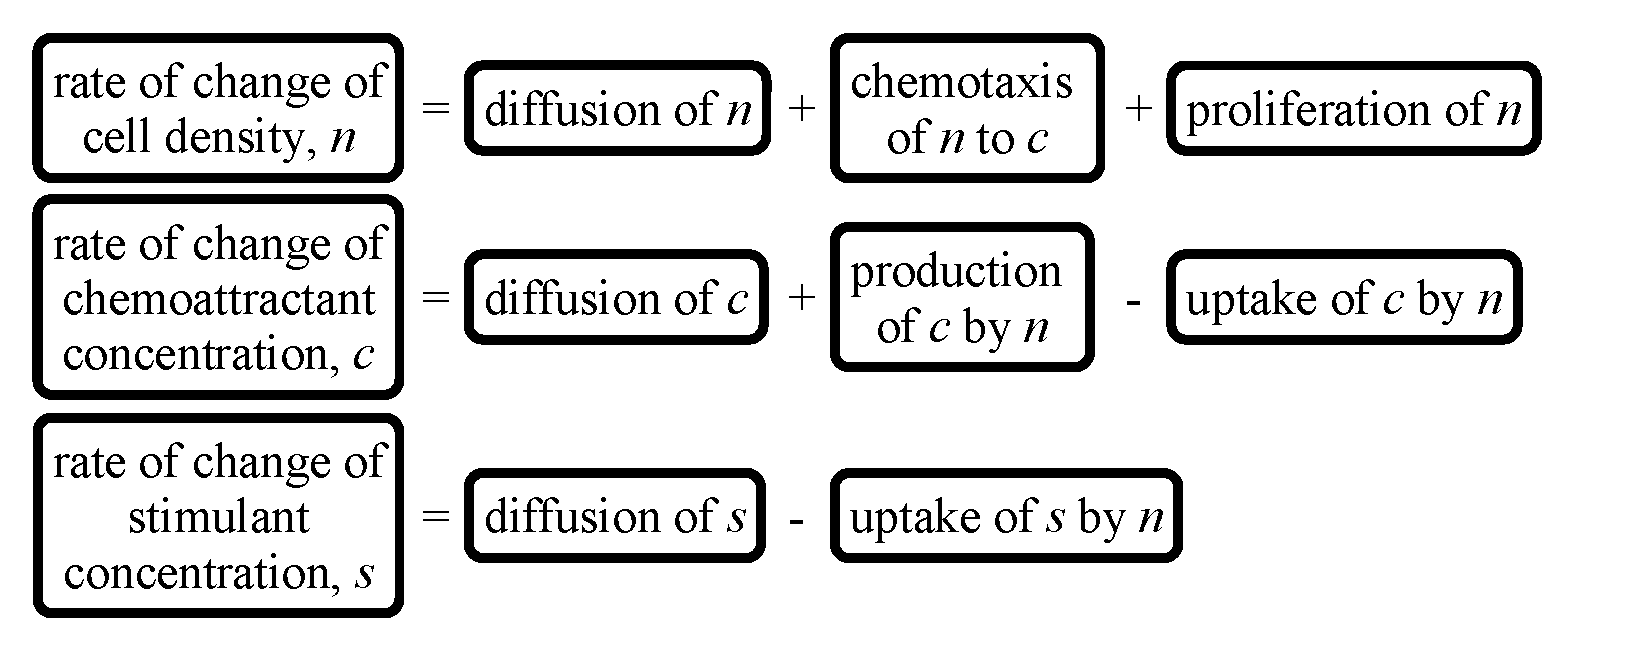
\includegraphics[width=\textwidth]{figures/bio/conceptual_model}
     \caption[Conceptual model of bacteria/chemoattractant/stimulant system.]{Conceptual model of bacteria/chemoattractant/stimulant system based on~\cite{spatial_patters_in_bio}.\label{fig:conceptual_model}}
   \end{center}
 \end{figure}

One possible mathematical model for bacterial chemotaxis is given by Murray et al.~\cite{spatial_patters_in_bio}:
% Bacterial chemotaxis: dimensional
\begin{align}
  \label{eq:pde_bio_n}
  \pdv{n}{t} & = D_n \Delta n - \grad{} \cdot \left[ \frac{k_1 n}{(k_2 + c)^2} \grad{c} \right]
                                    + k_3 n \left( k_4 \frac{s^2}{k_9 + s^2} - n \right) \\
  \label{eq:pde_bio_c}
  \pdv{c}{t} & = D_c \Delta c + k_5 s \frac{n^2}{k_6 + n^2} - k_7 nc \\
  \label{eq:pde_bio_s}
  \pdv{s}{t} & = D_s \Delta s - k_8 n \frac{s^2}{k_9 + s^2}
\end{align}
where $n$, $c$, and $s$ are the concentrations of bacteria, chemoattractant, and stimulant, respectively.  The remaining parameters govern the rates of proliferation, stimulant uptake, diffusion, and chemotaxis.  Some of these parameters have been measured experimentally, while others must be estimated. It should  be noted that the modeling of all right-hand-side terms in Equations~\eqref{eq:pde_bio_n}--\eqref{eq:pde_bio_s} other than diffusion is largely phenomenological in that other functional forms for these terms are plausible.  

Equation~\eqref{eq:pde_bio_n} describes the transport of bacteria.  The density of bacteria, $n$, may change through the physical processes of diffusion, chemotaxis, and proliferation.  These processes are described by the three terms on the right-hand-side of~\eqref{eq:pde_bio_n}.  Diffusion is the natural tendency for highly localized populations to spread out by moving in a direction away from the concentrated population (the direction opposite of the concentration gradient).  Conversely, chemotaxis is a process in which bacteria are attracted to regions of high chemoattractant density. In this case the bacteria move in the direction of increasing chemoattractant  (in the direction aligned with the chemoattractant gradient), hence chemotaxis may be thought of as an anti-diffusion process.  Finally, the proliferation of bacteria governs the growth or decay of a population in response to the local stimulant concentration. This term may be positive, negative, or zero depending on the local density of bacteria and stimulant.  In this way the proliferation term seeks to drive a given population into equilibrium with the available stimulant.

Equation~\eqref{eq:pde_bio_c} describes the transport of chemoattractant.  The three terms on the right-hand-side of the equation describe transport through diffusion, production, and depletion, respectively. The first term describes the familiar process of diffusion. The second term governs the production of chemoattractant which occurs when a bacteria concentration and stimulant are in contact.  This term is always positive or zero.  Conversely, the third term models depletion and may be negative or zero, depending upon local conditions.  This term represents the uptake of chemoattractant by bacteria.

Finally, Equation~\eqref{eq:pde_bio_s} governs the transport of stimulant.  In this model the local stimulant concentration may change through either diffusion or consumption.  There is no replenishing of stimulant in this model, although the degenerate case when $k_8=0$ corresponds to a fixed total amount of stimulant (for all time) whose spatial distribution may change only through diffusion.  In this case any initial stimulant distribution will tend to diffuse until it is distributed uniformly throughout the domain.

%\subsubsection{Nondimensionalization}
Equations~\eqref{eq:pde_bio_n}--\eqref{eq:pde_bio_s} can be scaled by introducing the following relationships~\cite{spatial_patters_in_bio}:
\\ %% 
\begin{minipage}[t]{.44\columnwidth}
  \begin{align}
    \hat{t} &= k_7 n_0 t \\
    u &= \frac{n}{n_0} \label{eq:bio_u_nondim}\\
    v &= \frac{c}{k_2} \\
    w &= \frac{s}{\sqrt{k_9}} \\
    \hat{\Delta} &= \frac{D_c}{k_7 n_0} \Delta \\
    d_u &= \frac{D_n}{D_c} \\
    d_w &= \frac{D_s}{D_c} 
  \end{align}
\end{minipage}
\hspace{.1\columnwidth}
\begin{minipage}[t]{.44\columnwidth}
  \begin{align}
    \alpha &= \frac{k_1}{k_2 D_c} \\
    \rho &= \frac{k_3}{k_7} \\
    \delta &= \frac{k_4}{n_0} \\
    \beta &= k_5 \frac{\sqrt{k_9}}{k_7 k_2 n_0} \\
    \kappa &= \frac{k_8}{k_7\sqrt{k_9}} \\
    \mu &= \frac{k_6}{n_0^2}
  \end{align}
\end{minipage}
\\
\\
which produces the nondimensional system
% Bacterial chemotaxis: nondimensional
\begin{align}
  \label{eq:pde_bio_u}
  \pdv{u}{\hat{t}} & = d_u \hat{\Delta} u - \alpha \grad{}\cdot \left[ \frac{u}{(1+ v)^2} \grad{v} \right]
                                    + \rho u \left( \delta \frac{w^2}{1 + w^2} - u \right) \\
  \label{eq:pde_bio_v}
  \pdv{v}{\hat{t}} & = \;\;\;\; \hat{\Delta} v + \beta w \frac{u^2}{\mu + u^2} - uv \\
  \label{eq:pde_bio_w}
  \pdv{w}{\hat{t}} & = d_w \hat{\Delta} w - \kappa u \frac{w^2}{1 + w^2}
\end{align}
For notational convenience the $\hat{()}$ will be dropped in the following sections.

%\subsubsection{Initial \& Boundary Conditions}
The initial conditions for the system are constructed to imitate a quiescent domain $\Omega$ with a given stimulant concentration $w_0$ at time $t=t_0$.  Since the domain initially is devoid of bacteria there is no initial chemoattractant concentration.  An initial inoculum of bacteria, $u_0$, is introduced and the solution evolves in response to this `disturbance.'  Specifically, for the problems that are considered subsequently
\begin{align}
  \label{eq:u0_bio}
  u_0 &= u(x,y), \;\; (x,y) \in \Omega \\
  \label{eq:v0_bio}
  v_0 &= 0 \\
  \label{eq:w0_bio}
  w_0 &= w(x,y), \;\; (x,y) \in \Omega
\end{align}
The actual implementation of initial conditions is an important issue.  Specifically, the initial conditions must be specified and implemented in a consistent way across a range of computational meshes.  This important aspect of the simulation will be addressed further in the application studies.

%\subsubsection{Boundary Conditions}
For a closed container with impermeable walls a physically sensible boundary condition for all variables in the system is 
\begin{align}
  \label{eq:du_dn_bio_eq_0}
  \pdv{u}{n} &= \grad{u}\cdot\nhat = 0 \\
  \label{eq:dv_dn_bio_eq_0}
  \pdv{v}{n} &= \grad{v}\cdot\nhat = 0 \\
  \label{eq:dw_dn_bio_eq_0}
  \pdv{w}{n} &= \grad{w}\cdot\nhat = 0
\end{align}
which simply states that there is no flux of bacteria, chemoattractant, or stimulant through the boundary of the domain~$\Omega$. %It will be seen in the following section that this boundary condition is particularly convenient to implement in the finite element discretization.



%%%%%%%%%%%%%%%%%%%%%%%%%%%%%%%%%%%%%%%%%%%%%%%%%%%%%%%%%%%%%%%%%%%%%%%%%%%%%%%
%\clearpage
\subsection{Weak Formulation}
The corresponding weighted-residual statement for equations~\eqref{eq:pde_bio_u}--\eqref{eq:pde_bio_v} follows from  multiplying each equation by a suitable test function~$\phi$ and integrating over the domain~$\Omega$, giving
\begin{align}
  \label{eq:weak_bio_u_preparts}
  \int_\Omega &\left[\pdv{u}{t} - d_u \Delta u + \alpha \grad{}\cdot \left[ \frac{u}{(1+ v)^2} \grad{v} \right]
                                    - \rho u \left( \delta \frac{w^2}{1 + w^2} - u \right)\right]\phi\dx  = 0 \\
  \label{eq:weak_bio_v_preparts}
  \int_\Omega &\left[\pdv{v}{t} - \Delta v - \beta w \frac{u^2}{\mu + u^2} + uv\right]\phi\dx = 0 \\
  \label{eq:weak_bio_w_preparts}
  \int_\Omega &\left[\pdv{w}{t} - d_w \Delta w + \kappa u \frac{w^2}{1 + w^2}\right]\phi\dx = 0
\end{align}
Applying Gauss' divergence theorem, selectively, and substituting \eqref{eq:du_dn_bio_eq_0}-\eqref{eq:dw_dn_bio_eq_0} in the resulting boundary integrals  yields the weak formulation: Find $\left(u,v,w\right)$ satisfying the specified initial conditions and
\begin{align}
  \int_\Omega& \left[\pdv{u}{t} - \rho u \left( \delta \frac{w^2}{1 + w^2} - u \right) \right]\phi\dx \nonumber \\
  \label{eq:weak_bio_u}
  &\;\;\;+ \int_\Omega \left[d_u \grad{u}\cdot\grad{\phi} - \alpha u \frac{\grad{v}\cdot\grad{\phi}}{(1+ v)^2} \right]\dx  = 0 \\  
  \label{eq:weak_bio_v}
  \int_\Omega& \left[\left(\pdv{v}{t} - \beta w \frac{u^2}{\mu + u^2} + uv\right)\phi + \grad{v}\cdot\grad{\phi}\right]\dx = 0 \\  
  \label{eq:weak_bio_w}
  \int_\Omega& \left[\left(\pdv{w}{t} + \kappa u \frac{w^2}{1 + w^2}\right)\phi + d_w\grad{w}\cdot\grad{\phi}\right]\dx = 0
\end{align}
for all admissible test functions $\phi$.  The weak statement~\eqref{eq:weak_bio_u}-\eqref{eq:weak_bio_w} implies \eqref{eq:pde_bio_u}-\eqref{eq:pde_bio_w} with \eqref{eq:du_dn_bio_eq_0}-\eqref{eq:dw_dn_bio_eq_0} as natural boundary conditions.
%This will starting point for the  finite element discretization discussed in the next section.

%Note that the boundary integrals in Equations~\eqref{eq:weak_bio_u}--\eqref{eq:weak_bio_w} (which result from integration by parts) have been omitted.  This is consistent with the no--flux boundary conditions imposed on the system.  Omitting these boundary integrals in~\eqref{eq:weak_bio_u}--\eqref{eq:weak_bio_w} naturally imposes these conditions in a weak sense.



%%%%%%%%%%%%%%%%%%%%%%%%%%%%%%%%%%%%%%%%%%%%%%%%%%%%%%%%%%%%%%%%%%%%%%%%%%%%%%%
\subsection{Finite Element Formulation}
The finite element formulation for~\eqref{eq:weak_bio_u}--\eqref{eq:weak_bio_w} follows upon replacing $\left(u,v,w\right)$ and $\phi$ with the finite dimensional approximations  $\left(u_h,v_h,w_h\right)$ and $\phi_h$.  Specifically, for a standard Lagrange finite element basis we have
\begin{align}
  \label{eq:bio_u_h}  
  u_h(\bv{x},t) &= \sum_{j=1}^N u_j(t) \phi_j(\bv{x}) \\
  \label{eq:bio_v_h}  
  v_h(\bv{x},t) &= \sum_{j=1}^N v_j(t) \phi_j(\bv{x}) \\
  \label{eq:bio_w_h}  
  w_h(\bv{x},t) &= \sum_{j=1}^N w_j(t) \phi_j(\bv{x}) 
\end{align}
where $u_j(t)$, $v_j(t)$, and $w_j(t)$ are the nodal values of the bacteria, chemoattractant, and stimulant at time $t$, respectively, and $N$ is the number of nodes in the domain. The corresponding discrete weak statement is then: find the approximate solution $\left(u_h,v_h,w_h\right)$ satisfying the specified initial conditions and 
\begin{align}
  \int_\Omega& \left[\pdv{u_h}{t} - \rho u_h \left( \delta \frac{w_h^2}{1 + w_h^2} - u_h \right) \right]\phi_h\dx \nonumber \\
  \label{eq:fe_bio_u}
  &\;\;\;+ \int_\Omega \left[d_u \grad{u_h}\cdot\grad{\phi_h} - \alpha u_h \frac{\grad{v_h}\cdot\grad{\phi_h}}{(1+ v_h)^2} \right]\dx  = 0 \\  
  \label{eq:fe_bio_v}
  \int_\Omega& \left[\left(\pdv{v_h}{t} - \beta w_h \frac{u_h^2}{\mu + u_h^2} + u_h v_h\right)\phi_h + \grad{v_h}\cdot\grad{\phi_h}\right]\dx = 0 \\ 
  \label{eq:fe_bio_w}
  \int_\Omega& \left[\left(\pdv{w_h}{t} + \kappa u_h \frac{w_h^2}{1 + w_h^2}\right)\phi + d_w\grad{w_h}\cdot\grad{\phi_h}\right]\dx = 0
\end{align}
for all admissible test functions $\phi_h$.  This discrete approximation to \eqref{eq:weak_bio_u}-\eqref{eq:weak_bio_w} forms the basis of the computational model described in the next section.


%%%%%%%%%%%%%%%%%%%%%%%%%%%%%%%%%%%%%%%%%%%%%%%%%%%%%%%%%%%%%%%%%%%%%%%%%%%%%%%
\section{Solution Methodology}
Equations~\eqref{eq:pde_bio_u}--\eqref{eq:pde_bio_w} form a highly coupled, transient,  nonlinear system.  Furthermore, the system evolution occurs over a disparate range of time scales that must be captured accurately.  This section outlines the techniques employed in the present work to solve the system of equations.

%%%%%%%%%%%%%%%%%%%%%%%%%%%%%%%%%%%%%%%%%%%%%%%%%%%%%%%%%%%%%%%%%%%%%%%%%%%%%%%
\subsection{Time Integration}
The time integration method used in this work can be developed by considering the generic first-order ordinary differential equation
\begin{equation}
  \label{eq:udot_eq_f_u}
  \bv{\dot{u}} = \bv{f}\left(t,\bv{u}\left(t\right)\right),\;\; t>t_0,\;\; \bv{u}\left(t_0\right) = \bv{u}_0
\end{equation}
Explicit methods for~\eqref{eq:udot_eq_f_u} are simple to formulate and the computational cost per step is low.  The price for this simplicity is decreased stability.  Consequently, limits must be posed on the integration step size $\Delta t$ in an explicit scheme.  Implicit methods, on the other hand, are typically stable for any $\Delta t$ but are considerably more difficult to implement and have a higher computational cost per time step.  A combined explicit Adams-Bashforth predictor and implicit Trapezoidal corrector with step control are applied in the present work and are discussed next.

%%%%%%%%%%%%%%
\subsubsection*{Adams-Bashforth Explicit Scheme}
The Adams--Bashforth explicit integration formula applied to Equation~\eqref{eq:udot_eq_f_u} is given by
\begin{equation}
  \label{eq:ab_expl_cont}
  \bv{u}\left(t+\Delta t\right) = \bv{u}_n +
    \frac{\Delta t}{2}\left[\left(2 + \frac{\Delta t_n}{\Delta t_{n-1}}\right)\bv{f}_n -
                            \left(\frac{\Delta t_n}{\Delta t_{n-1}}\right)\bv{f}_{n-1}\right] +
     \mathcal{O}\left(\Delta t^2\right)
\end{equation}
where $\bv{u}_n=\bv{u}\left(t_n\right)$, $\Delta t_n = t_n - t_{n-1}$, and $\bv{f}_n = \bv{f}\left(t_n, \bv{u}\left(t_n\right)\right)$.  This  can be used to give a second--order accurate approximation for $\bv{u}_{n+1}$ by ignoring the error terms $\mathcal{O}\left(\Delta t^2\right)$
\begin{equation}
  \label{eq:ab_expl_f}
  \bv{u}_{n+1} = \bv{u}_n +
    \frac{\Delta t_{n+1}}{2}\left[\left(2 + \frac{\Delta t_n}{\Delta t_{n-1}}\right)\bv{f}_n -
                            \left(\frac{\Delta t_n}{\Delta t_{n-1}}\right)\bv{f}_{n-1}\right]
\end{equation}
Substituting Equation~\eqref{eq:udot_eq_f_u} into Equation~\eqref{eq:ab_expl_f} gives the equivalent form
\begin{equation}
  \label{eq:ab_expl}
  \bv{u}_{n+1} = \bv{u}_n +
    \frac{\Delta t_{n+1}}{2}\left[\left(2 + \frac{\Delta t_n}{\Delta t_{n-1}}\right)\bv{\dot{u}}_n -
                            \left(\frac{\Delta t_n}{\Delta t_{n-1}}\right)\bv{\dot{u}}_{n-1}\right]
\end{equation}

%%%%%%%%%%%%%%%
\subsubsection*{Trapezoidal Rule Implicit Scheme}
The implicit trapezoidal integration rule applied to Equation~\eqref{eq:udot_eq_f_u} is given by
\begin{equation}
  \label{eq:tr_impl_cont}
  \bv{u}\left(t+\Delta t\right) = \bv{u}_n + \frac{\Delta t}{2}\left(\bv{f}\left(t+\Delta t\right) + \bv{f}_n\right)
  + \mathcal{O}\left(\Delta t^2\right)
\end{equation}
which yields the second order accurate scheme for $\bv{u}_{n+1}$
\begin{equation}
  \label{eq:tr_impl_f}
  \bv{u}_{n+1} = \bv{u}_n + \frac{\Delta t_{n+1}}{2}\left(\bv{f}_{n+1} + \bv{f}_n\right)
\end{equation}
or equivalently
\begin{equation}
  \label{eq:tr_impl_u}
  \bv{u}_{n+1} = \bv{u}_n + \frac{\Delta t_{n+1}}{2}\left(\bv{\dot{u}}_{n+1} + \bv{\dot{u}}_n\right)
\end{equation}

This scheme is implicit because of its dependence on the unknown value $\bv{f}_{n+1}$.  Furthermore, for the class of problems considered in this work $\bv{f}=\bv{f}(\bv{u})$ and is highly nonlinear.  Therefore, using Equation~\eqref{eq:tr_impl_f} requires the solution of a nonlinear implicit system of equations using the techniques described in Section~\ref{sect:bio_linearization}.

%%%%%%%%%%%%%%
\subsubsection*{Local Error Control}
An important benefit of the two stage predictor--corrector algorithm is that it provides a means to estimate the local error incurred at a given time step~\cite{iserles_numerical_analysis}.  Consider $\bv{\hat{u}}_{n+1}$ and $\bv{u}_{n+1}$ as predictor and corrector calculations, respectively, both of which approximate the exact solution $\bv{u}\left(t_{n+1}\right)$ to $\mathcal{O}(p)$ accuracy.  The truncation errors for these approximate solutions are defined as
\begin{align}
  \label{eq:ab_error}
  \bv{\hat{\tau}}_{n+1} &\equiv \bv{u}\left(t_{n+1}\right) - \bv{\hat{u}}_{n+1} = \hat{c} \Delta t_{n+1}^{p+1} \bv{u}^{(p+1)}\left(t_{n+1}\right) + \mathcal{O}\left(\Delta t_{n+1}^{p+2}\right) \\
  \label{eq:tr_error}
  \bv{\tau}_{n+1} &\equiv \bv{u}\left(t_{n+1}\right) - \bv{u}_{n+1} = c \Delta t_{n+1}^{p+1} \bv{u}^{(p+1)}\left(t_{n+1}\right) + \mathcal{O}\left(\Delta t_{n+1}^{p+2}\right)
\end{align}
Subtracting~\eqref{eq:ab_error} from~\eqref{eq:tr_error} and ignoring higher order terms yields
\begin{align}
  \nonumber
   \bv{\hat{u}}_{n+1} - \bv{u}_{n+1} &\approx \left(c - \hat{c}\right)\Delta t_{n+1}^{p+1} \bv{u}^{(p+1)}\left(t_{n+1}\right) \\
   \label{eq:u_pp1_approx}
   \Delta t_{n+1}^{p+1} \bv{u}^{(p+1)}\left(t_{n+1}\right) &\approx \frac{\bv{\hat{u}}_{n+1} - \bv{u}_{n+1}}{c - \hat{c}}
\end{align}
Substituting~\eqref{eq:u_pp1_approx} into~\eqref{eq:tr_error} provides an estimation of the local truncation error $\bv{\tau}_{n+1}$
\begin{equation}
  \label{eq:u_np1_error}
  \bv{\tau}_{n+1} \approx \frac{c}{c - \hat{c}}\left(\bv{\hat{u}}_{n+1} - \bv{u}_{n+1}\right)
\end{equation}
which, for the Adams--Bashforth predictor/trapezoidal rule corrector pair employed in the present work  becomes
\begin{equation}
  \label{eq:u_np1_ab_tr_error}
  \bv{\tau}_{n+1} \approx \frac{\bv{\hat{u}}_{n+1} - \bv{u}_{n+1}}{3\left(1 + \Delta t_n/\Delta t_{n+1}\right)}
\end{equation}
Finally, Equation~\eqref{eq:tr_error} yields the following relationship for the truncation error at successive time steps
\begin{equation}
  \label{eq:tau_np2_ratio}
  \frac{\|\bv{\tau}_{n+2}\|}{\|\bv{\tau}_{n+1}\|} \approx \left(\frac{\Delta t_{n+2}}{\Delta t_{n+1}}\right)^{3}
\end{equation}
which can be used to provide an estimate for the time step $\Delta t_{n+2}$ required to limit $\|\bv{\tau}_{n+2}\|$ to some specified value $\varepsilon_t$
\begin{equation}
  \label{eq:dt_comp}
  \Delta t_{n+2} = \Delta t_{n+1} \left(\frac{\varepsilon_t}{\| \bv{\tau}_{n+1}\|}\right)^{1/3}
\end{equation}

%%%%%%%%%%%%%%%
\subsubsection*{Predictor--Corrector Algorithm}
%The simplicity of the Adams--Bashforth explicit algorithm and the stability of the implicit trapezoidal rule can be combined in a predictor--corrector algorithm.
The general approach is to use the explicit Adams--Bashforth step given by Equation~\eqref{eq:ab_expl} to predict $\bv{\hat{u}}_{n+1}$.  This predicted value is then used as the initial iterate to solve the nonlinear system in Equation~\eqref{eq:tr_impl_f} via Newton iteration (as described in the next section).  The algorithm is outlined as follows:
\begin{enumerate}
  \tightlist
  %
  \item Predict the solution $\bv{\hat{u}}_{n+1}$ at $t_{n+1}$ using Equation~\eqref{eq:ab_expl}:
    \begin{equation}
      %\label{eq:ab_pred}
      \nonumber
      \bv{\hat{u}}_{n+1} = \bv{u}_n +
      \frac{\Delta t_{n+1}}{2}\left[\left(2 + \frac{\Delta t_n}{\Delta t_{n-1}}\right)\bv{\dot{u}}_n -
        \left(\frac{\Delta t_n}{\Delta t_{n-1}}\right)\bv{\dot{u}}_{n-1}\right]
    \end{equation}
  %
  \item Solve Equation~\eqref{eq:tr_impl_f} using the predicted solution $\bv{\hat{u}}_{n+1}$ as the initial guess for the nonlinear implicit solver.

  %
  \item Estimate the truncation error $\|\bv{\tau}_{n+1}\|$ using~\eqref{eq:u_np1_ab_tr_error} and compute the next time step $\Delta t_{n+2}$ using~\eqref{eq:dt_comp}:
    \begin{align}
      \nonumber
      \|\bv{\tau}_{n+1}\| &= \frac{\|\bv{\hat{u}}_{n+1} - \bv{u}_{n+1}\|}{3\left(1 + \Delta t_n/\Delta t_{n+1}\right)} \\
      \nonumber
      \Delta t_{n+2} &= \Delta t_{n+1} \left(\frac{\varepsilon_t}{\| \bv{\tau}_{n+1}\|}\right)^{1/3}
    \end{align}
    
  %
  \item Update the time derivative by inverting Equation~\eqref{eq:tr_impl_u}
    \begin{equation}
      %\label{eq:udot_update}
      \nonumber
      \bv{\dot{u}}_{n+1} = \frac{2}{\Delta t_{n+1}} \left(\bv{u}_{n+1} - \bv{u}_n\right) - \bv{\dot{u}}_n
    \end{equation}

  %
  \item Terminate the integration when the change between successive time steps is less than some
    specified tolerance $\varepsilon_{ss}$
    \begin{equation}
      \label{eq:ss_terminate}
      \|\bv{u}_{n+1} - \bv{u_n}\| < \varepsilon_{ss} \|\bv{u}_{n+1}\|
    \end{equation}
\end{enumerate}


%%%%%%%%%%%%%%%%%%%%%%%%%%%%%%%%%%%%%%%%%%%%%%%%%%%%%%%%%%%%%%%%%%%%%%%%%%%%%%%
\subsection{Linearization \label{sect:bio_linearization}}
This section addresses the solution of the nonlinear system of equations which results from the implicit time discretization. To develop the nonlinear solution scheme it is useful to recast Equation~\eqref{eq:tr_impl_f} in residual form as
\begin{equation}
  \label{eq:bio_residual}
  \bv{R}\left(\bv{u}_{n+1}\right) \equiv \frac{\bv{u}_{n+1}-\bv{u}_n}{\Delta t_{n+1}} - \frac{\bv{f}\left(\bv{u}_{n+1}\right) + \bv{f}\left(\bv{u}_n\right)}{2} = 0
\end{equation}
where $\bv{u}_{n+1}$ is the unknown solution at time $t_{n+1}s$.  Newton's method can be derived for this system by considering a Taylor series applied to Equation~\eqref{eq:bio_residual}
\begin{equation}
  \label{eq:bio_taylor_series}
  \bv{R}\left(\bv{u_{n+1}} + \delta\bv{u}_{n+1}\right) =
    \bv{R}\left(\bv{u}_{n+1}\right) +
    \pdv{\bv{R}}{\bv{u}}\Big|_{\bv{u}_{n+1}}\delta\bv{u}_{n+1} +
    \mathcal{O}\left(\delta\bv{u}_{n+1}^2\right)
\end{equation}
where $\partial\bv{R}/\partial\bv{u}$ is the Jacobian matrix for the system.  Ignoring higher order terms and requiring $\bv{R}\left(\bv{u}_{n+1} + \delta\bv{u}_{n+1}\right)=0$  produces Newton's method
\begin{equation}
  \label{eq:bio_newtons_method}
  \pdv{\bv{R}}{\bv{u}}\Big|_{\bv{u}_{n+1}^l}\delta\bv{u}_{n+1}^{l+1} =
    -\bv{R}\left(\bv{u}_{n+1}^l\right)
\end{equation}
or equivalently 
\begin{equation}
  \label{eq:bio_newtons_method_iterative}
  \pdv{\bv{R}}{\bv{u}}\Big|_{\bv{u}_{n+1}^l}\bv{u}_{n+1}^{l+1} =
  \pdv{\bv{R}}{\bv{u}}\Big|_{\bv{u}_{n+1}^l}\bv{u}_{n+1}^{l}-\bv{R}\left(\bv{u}_{n+1}^l\right)
\end{equation}
where $\bv{u}_{n+1}^l$ is an intermediate iterate which approximates the unknown root $\bv{u}_{n+1}$.
The nonlinear system is then solved as a sequence of linear approximations as follows:
\begin{enumerate}
  \tightlist
  \item Let $l=0,\;\bv{u}_{n+1}^l=\bv{\hat{u}}_{n+1}$
  \item Solve the linear system~\eqref{eq:bio_newtons_method_iterative} for $\bv{u}_{n+1}^{l+1}$
  \item Stop if $\|\bv{u}_{n+1}^{l+1}-\bv{u}_{n+1}^l\|<\varepsilon_{nl}$%, setting $\bv{u}_{n+1}=\bv{u}^{l+1}$
  \item Else increment $l$ and repeat from step~2
\end{enumerate}

Newton's method exhibits quadratic convergence provided that the initial iterate $\bv{u}_{n+1}^0$ is sufficiently close to the root $\bv{u}_{n+1}$.  If this condition is not met then the iteration may converge at a sub-optimal rate or fail to converge altogether.  In this work the Adams--Bashforth predicted solution is taken as the initial guess and nonlinear convergence is typically obtained in three or four iterations.  If for some reason the nonlinear scheme fails to converge within a specified number of iterations the time step is halved and the process is repeated.  This successive step--halving should ensure that the predicted solution is eventually close enough to the unknown root for the method to converge.



%%%%%%%%%%%%%%%%%%%%%%%%%%%%%%%%%%%%%%%%%%%%%%%%%%%%%%%%%%%%%%%%%%%%%%%%%%%%%%%
\subsection{Adaptive Mesh Refinement}
As mentioned in the introduction, the presence of highly localized features such as propagating ``fronts'' and isolated, stationary ``spots'' makes this application class particularly well-suited to simulation with adaptive mesh refinement  techniques.  This section provides an overview of the algorithm used to automatically adapt the mesh to a particular solution.

The AMR algorithm requires a candidate solution on a particular mesh as input.  The error in this candidate solution is then estimated in some way.  The algorithm will then selectively coarsen and refine the mesh in areas of relatively low and high error, respectively.  The end goal is to produce a mesh which equidistributes the error.  Note that the current software implementation can only coarsen cells which have previously been refined, so it is not possible to coarsen the mesh below its initial resolution.

The gradient-based error indicator described in Section~\ref{sec:error_indicators} is used here to select which elements will be coarsened and refined at each step in the adaptive process.  The gradient-based indicator is very effective at locating regions of high curvature in the solution field.
This indicator is applied to all variables in the system, resulting in a discrete value for each element in the simulation.

The mean and standard deviation of this distribution is then calculated.  User-specified refinement and coarsening fractions of the standard deviation are then added and subtracted from the mean, respectively, to find threshold values for coarsening and refinement.  Any element whose error is less than the coarsening threshold is considered a candidate for coarsening.  All elements whose error is greater than the refinement threshold will be refined, provided they do not exceed a user-specified maximum refinement level.



%\subsubsection{Error Indicators}

%\subsubsection{Element Selection}

%%%%%%%%%%%%%%%%%%%%%%%%%%%%%%%%%%%%%%%%%%%%%%%%%%%%%%%%%%%%%%%%%%%%%%%%%%%%%%%
\subsection{Solution Algorithm}
The numerical methods described in the preceding sections are combined into the solution algorithm outlined in Algorithm~\ref{alg:bio_algorithm}.
\begin{algorithm}[!htb]
  \caption{Transient adaptive nonlinear solution algorithm used for chemotactic \emph{E.coli} systems\label{alg:bio_algorithm}}
 \noindent
  \centering
    \begin{minipage}{.95\textwidth}
      \noindent
      \sffamily
      \setcounter{alines}{0}
      \begin{list}{\arabic{alines}:\ \ }{\usecounter{alines}}
        \renewcommand{\baselinestretch}{1.0} \setlength{\itemsep}{-1ex}
        \item Interpolate initial conditions
	\item $\bv{u}^0 = \bv{u}(\bv{x},t)$ 
        \item \textbf{for} $n=1$ to $N_\text{time steps}$ \textbf{do}
	\item \ \ \ Predict $\hat{\bv{u}}^n$ using~\eqref{eq:ab_expl}
	\item \ \ \ Let $\tilde{\bv{u}}^n = \hat{\bv{u}}^n$
	\item \ \ \ Solve the nonlinear system for $\tilde{\bv{u}}^n$:
 	\item \ \ \ \textbf{do}
 	\item \ \ \ \ \ \ Form system matrix $\bt{K} = \bt{K}(\tilde{\bv{u}}^n,\bv{u}^{n-1})$
 	\item \ \ \ \ \ \ Form system vector $\bv{f}= \bv{f}(\tilde{\bv{u}}^n,\bv{u}^{n-1})$
 	\item \ \ \ \ \ \ Solve the linear system $\bt{K} \; \delta\tilde{\bv{u}}^n = \bv{f}$
	\item \ \ \ \ \ \ Update the solution $\tilde{\bv{u}}^n \leftarrow \tilde{\bv{u}}^n + \delta\tilde{\bv{u}}^n$
 	\item \ \ \ \textbf{while} $\norm[\infty]{\delta\tilde{\bv{u}}^n} < \varepsilon_{nl}$
	\item \ \ \ Compute error indicator for each element using $\tilde{\bv{u}}^n$
	\item \ \ \ \textbf{if} error is acceptable
	\item \ \ \ \ \ \ Let $\bv{u}^n=\tilde{\bv{u}}^n$
        \item \ \ \ \textbf{else}
	\item \ \ \ \ \ \ Refine and coarsen mesh
	\item \ \ \ \ \ \ Project $\Pi\tilde{\bv{u}}^n\rightarrow\bv{u}^n,\;\Pi\tilde{\bv{u}}^{n-1}\rightarrow\bv{u}^{n-1}$
	\item \ \ \ \ \ \ Solve the nonlinear system for $\bv{u}^n$:
 	\item \ \ \ \ \ \ \textbf{do}
 	\item \ \ \ \ \ \ \ \ \ Form system matrix $\bt{K} = \bt{K}(\bv{u}^n,\bv{u}^{n-1})$
 	\item \ \ \ \ \ \ \ \ \ Form system vector $\bv{f}= \bv{f}(\bv{u}^n,\bv{u}^{n-1})$
 	\item \ \ \ \ \ \ \ \ \ Solve the linear system $\bt{K} \; \delta\bv{u}^n = \bv{f}$
	\item \ \ \ \ \ \ \ \ \ Update the solution $\bv{u}^n \leftarrow \bv{u}^n + \delta\bv{u}^n$
 	\item \ \ \ \ \ \ \textbf{while} $\norm[\infty]{\delta\bv{u}^n} < \varepsilon_{nl}$
        \item \ \ \ \textbf{endif}
        \item \textbf{end} \\
      \end{list}
    \end{minipage}
\end{algorithm}
This is the basic solution procedure that is applied in the following section to a number of application studies.

%%\begin{figure}[!htb]
%%  \noindent
%%  \centering
%%  \framebox{
%%    \begin{minipage}{.95\textwidth}
%%      \noindent
%%      \sffamily
%%      \newcounter{alines}
%%      \begin{list}{\arabic{alines}:\ \ }{\usecounter{alines}}
%%        \renewcommand{\baselinestretch}{1.0} \setlength{\itemsep}{-1ex}
%%        \item Compute initial residual:
%%        $\lav{r}_0=\lav{b}-\lam{A}\lav{x}_0$
%%        \item Let $\bar{\lav{r}} = \lav{r}_0$
%%        \item \textbf{for} $k=1$ to $n_\text{iter}$ \textbf{do}
%%        \item \ \ \ $\rho_{k-1} = \bar{\lav{r}}^\text{T}\lav{r}_{k-1}$
%%        \item \ \ \ \textbf{if} $\rho_{k-1} = 0$ method fails
%%        \item \ \ \ \textbf{if} $k=1$
%%        \item \ \ \ \ \ \ $\lav{p}_k = \lav{r}_{k-1}$
%%        \item \ \ \ \textbf{else}
%%        \item \ \ \ \ \ \ ${\beta = (\rho_{k-1}/\rho_{k-2})
%%          (\alpha_{k-1}/\omega_{k-1})}$
%%        \item \ \ \ \ \ \ ${\lav{p}_k = \lav{r}_{k-1} +
%%          \beta(\lav{p}_{k-1} - \omega_{k-1} \lav{w}_{k-1})}$
%%        \item \ \ \ \textbf{endif}
%%        \item \ \ \ Apply Preconditioning by solving ${\lam{Q}
%%          \hat{\lav{p}} = \lav{p}_k}$
%%        \item \ \ \ $\lav{w}_k = \lam{A}\hat{\lav{p}}$
%%        \item \ \ \ $\alpha_k = \rho_{k-1}/(\bar{\lav{r}},\lav{w}_k)$
%%        \item \ \ \ $\lav{s}=\lav{r}_{k-1}-\alpha_k \lav{w}_k$
%%        \item \ \ \ Stop if $\norm{s} < \epsilon_\text{L} \norm{b} $
%%        \item \ \ \ Apply Preconditioning by solving ${\lam{Q}
%%          \hat{\lav{s}} = \lav{s}}$
%%        \item \ \ \ $\lav{t} = \lam{A}\hat{\lav{s}}$
%%        \item \ \ \ ${\omega_k = \lav{t}^\text{T}\lav{s} /
%%          \lav{t}^\text{T}\lav{t}}$  
%%        \item \ \ \ ${\lav{x}_k = \lav{x}_{k-1} + \alpha_k\hat{\lav{p}}_k
%%          + \omega_k\hat{\lav{s}}}$
%%        \item \ \ \ $\lav{r}_k = \lav{s} - \omega_k \lav{t}$
%%        \item \ \ \ Stop if $\norm{\lav{r}_k} < \epsilon_\text{L}
%%        \norm{b} $
%%        \item \textbf{end} \\
%%      \end{list}
%%    \end{minipage}
%%  }
%%\caption{BCGStab Algorithm\label{fig:bcgstab}}
%%\end{figure}



%%%%%%%%%%%%%%%%%%%%%%%%%%%%%%%%%%%%%%%%%%%%%%%%%%%%%%%%%%%%%%%%%%%%%%%%%%%%%%%
\clearpage
\section{Application Studies}

%%%%%%%%%%%%%%%%%%%%%%%%%%%%%%%%%%%%%%%%%%%%%%%%%%%%%%%%%%%%%%%%%%%%%%%%%%%%%%%
\subsection{Continuous Concentric Advancing Rings\label{sec:concentric_rings}}
\subsubsection{Domain Specification and Initial Conditions}

The first biological transport application investigated here corresponds to the case of relatively weak chemotaxis in the presence of strong diffusion.  The initial conditions for this problem physically correspond to an initial inoculum of bacteria located at the center of a square domain defined as $\Omega=[-20,20]^2$.  The domain is initially devoid of chemoattractant and has a uniform stimulant distribution. By assuming symmetry of the spatial pattern with respect to the $x$ and $y$ axes it is possible to simulate only the quarter-domain $\hat{\Omega}=[0,20]^2$, thus reducing the number of unknowns in the approximate solution by a factor of four.

In Equation~\eqref{eq:bio_u_nondim} the physical bacteria concentration ($n$) is normalized by some reference concentration ($n_0$). The resulting initial concentration for this case is $u_0=5$.  It is important that $u_0$ be specified in such a way that it can be implemented consistently across a range of mesh resolutions and element types so that mesh refinement studies may be performed with consistent initial data.  This is especially true for reactive systems such as~\eqref{eq:pde_bio_u}--\eqref{eq:pde_bio_w} which are extremely sensitive to initial values in the sense that slightly perturbed initial conditions can evolve into markedly different states~\cite{modelling_error}.

The present work uses a sequence of uniformly refined meshes with both bilinear and biquadratic elements to assess mesh convergence.  The coarsest mesh contains $100\times100$ elements, yielding a coarse mesh spacing of $h_c=0.2$. For this family of meshes the initial conditions are taken as a tensor product of the following one-dimensional distributions, which may be represented exactly on all meshes used in this study:

\begin{alignat}{2}
  u_0 & = 5                   & \qquad & x \le h_c     \label{eq:u0_1_concentric_rings} \\
      & = 10 - \frac{5x}{h_c} & \qquad & h_c < x < 2hc \label{eq:u0_2_concentric_rings} \\
      & =0                    & \qquad & x \ge 2hc     \label{eq:u0_3_concentric_rings} \\
      &                       &        & \nonumber \\  
  v_0 & =0                    &        &               \label{eq:v0_concentric_rings}   \\
      &                       &        & \nonumber \\  
  w_0 & =5                    &        &               \label{eq:w0_concentric_rings}   
\end{alignat}
The resulting two-dimensional initial bacteria concentration is shown in Figure~\ref{fig:u0_concentric_rings}.
\begin{figure}[hbtp]
  \begin{center}
    \includegraphics[width=\textwidth]{figures/bio_concentric_rings/u0_schematic}
    \caption{Initial bacteria concentration for the concentric ring problem\label{fig:u0_concentric_rings}}
  \end{center}
\end{figure}
In particular, the linear decay of initial bacteria concentration specified by Equation~\eqref{eq:u0_2_concentric_rings} is chosen because it can be represented exactly with the bilinear and biquadratic elements for the full range of mesh resolutions used in this study.
Also, by fixing the slope of the decay for all mesh resolutions, initial transients caused by inconsistent initial conditions are avoided.  Numerical experiments have shown that failing to maintain consistent initial conditions for reactive transport applications can yield markedly different dynamics in the system. 

\subsubsection{System Parameters}
The relevant parameters for this case were taken from Woodward et~al.~\cite{spatio_temporal_patterns} and are listed in Table~\ref{table:concentric_rings_parameters}.% Parameter values - biological problem no. 1:  concentric rings
\begin{table}[hbtp]
  \begin{center}
    \caption[Nondimensional parameter values for concentric rings]{Nondimensional parameter values for concentric rings (from Woodward et~al.~\cite{spatio_temporal_patterns})}
    \label{table:concentric_rings_parameters}
    \vspace{1em}
    \begin{tabular}{cccccccc} \hline \hline
      $\bv{d_u}$ & $\bv{d_w}$ & $\bv{\alpha}$ & $\bv{\beta}$ & $\bv{\delta}$ & $\bv{\rho}$ & $\bv{\mu}$ & $\bv{\kappa}$ \\
      \unitfrac{1}{4}       & 1          &  7            & 10           & 10            & \unitfrac{1}{10}         & 250         & 0             \\ \hline
    \end{tabular}
  \end{center}
\end{table}
The particular choice $\alpha=7$ de-emphasizes the influence of chemotaxis in comparison to problems considered subsequently.  Put another way, this problem is more sensitive to transport via reaction and diffusion than chemotaxis. For this choice of parameters equations~\eqref{eq:pde_bio_u}--\eqref{eq:pde_bio_w} become
% Bacterial chemotaxis: concentric rings problem, 1st simplification
\begin{align}
  \label{eq:pde_bio_u_concentric_rings_1}
  \frac{\partial u}{\partial t} & = \frac{1}{4} \Delta u - 7 \; \grad{}\cdot \left[ \frac{u}{(1+ v)^2} \grad{v} \right]
                                    + \frac{u}{10} \left( \frac{10 \; w^2}{1 + w^2} - u \right) \\
  \label{eq:pde_bio_v_concentric_rings_1}
  \frac{\partial v}{\partial t} & = \;\;\Delta v + \frac{10 \; w u^2}{250 + u^2} - uv \\
  \label{eq:pde_bio_w_concentric_rings_1}
  \frac{\partial w}{\partial t} & = \;\;\Delta w 
\end{align}
In particular, the parameter $\kappa=0$ decouples the stimulant concentration ($w$) from the bacterial ($u$) and chemoattractant ($v$) concentrations. The physical interpretation of this scenario is that the stimulant supply is essentially unlimited, and its distribution is influenced only though diffusion.  Specifically, the bacteria cannot deplete the stimulant source, no matter how densely populated a region may be.  Additionally, since the stimulant is uniformly distributed initially, even diffusion will be absent for this particular case.  In this scenario the stimulant distribution is completely defined by its initial value, and the governing equations reduce to
% Bacterial chemotaxis: concentric rings problem, 2nd simplification
\begin{align}
  \label{eq:pde_bio_w_concentric_rings_2}
  w &= 5 \\
  \label{eq:pde_bio_u_concentric_rings_2}
  \frac{\partial u}{\partial t} & = \frac{1}{4} \Delta u - 7 \; \grad{}\cdot \left[ \frac{u}{(1+ v)^2} \grad{v} \right]
                                    + u \left( \frac{25}{26} - \frac{u}{10} \right) \\
  \label{eq:pde_bio_v_concentric_rings_2}
  \frac{\partial v}{\partial t} & = \;\;\Delta v + \frac{50 \; u^2}{250 + u^2} - uv
\end{align}
It is worth noting that the decoupling of the governing equations when $\kappa=0$ could be exploited numerically.  In this case the system Jacobian required in the nonlinear solution scheme is smaller than the general case because $\partial R_u/\partial w$, $\partial R_v/\partial w$, $\partial R_w/\partial u$, and $\partial R_w/\partial v$ are identically zero, hence no storage needs to be allocated for these terms.

\subsubsection{Results}
For the parameter set considered in this problem (see Table~\ref{table:concentric_rings_parameters}), the system forms a pattern of concentric rings which grow in number as a function of time until the domain is filled. Figure~\ref{fig:bio_concentric_rings_bacteria} shows a time sequence of bacterial concentration.  The chemoattractant concentration for the same points in time is shown in Figure~\ref{fig:bio_concentric_rings_chemoattractant}. This concentric ring pattern is similar to the top left experimental image shown in Figure~\ref{fig:ecoli_patterns_nature}.
\begin{figure}
  \begin{center}
    \subfigure[t=15.0]{\includegraphics[height=.25\textheight]{figures/bio_concentric_rings/u_00012}}
    \subfigure[t=17.5]{\includegraphics[height=.25\textheight]{figures/bio_concentric_rings/u_00014}} \\
    \subfigure[t=20.0]{\includegraphics[height=.25\textheight]{figures/bio_concentric_rings/u_00016}}
    \subfigure[t=22.5]{\includegraphics[height=.25\textheight]{figures/bio_concentric_rings/u_00018}} \\
    \subfigure[t=25.0]{\includegraphics[height=.25\textheight]{figures/bio_concentric_rings/u_00020}}
    \subfigure[t=27.5\label{fig:bio_concentric_rings_bacteria_t27.5}]{\includegraphics[height=.25\textheight]{figures/bio_concentric_rings/u_00022}}
    \caption{Continuous concentric advancing rings. Bacteria concentration history.\label{fig:bio_concentric_rings_bacteria}}
  \end{center}
\end{figure}

\begin{figure}
  \begin{center}
    \subfigure[t=15.0]{\includegraphics[height=.25\textheight]{figures/bio_concentric_rings/v_00012}}
    \subfigure[t=17.5]{\includegraphics[height=.25\textheight]{figures/bio_concentric_rings/v_00014}} \\
    \subfigure[t=20.0]{\includegraphics[height=.25\textheight]{figures/bio_concentric_rings/v_00016}}
    \subfigure[t=22.5]{\includegraphics[height=.25\textheight]{figures/bio_concentric_rings/v_00018}} \\
    \subfigure[t=25.0]{\includegraphics[height=.25\textheight]{figures/bio_concentric_rings/v_00020}}
    \subfigure[t=27.5\label{fig:bio_concentric_rings_chemoattractant_t27.5}]{\includegraphics[height=.25\textheight]{figures/bio_concentric_rings/v_00022}}
    \caption{Continuous concentric advancing rings. Chemoattractant concentration history.\label{fig:bio_concentric_rings_chemoattractant}}
  \end{center}
\end{figure}

It is interesting to note that the spatial pattern shown in the figures exhibits radial symmetry.  It is not immediately obvious that this would be the case, especially given the clearly two-dimensional nature of the initial conditions (c.f. Figure~\ref{fig:u0_concentric_rings}).  Figure~\ref{fig:bio_concentric_rings_startup} details the initial transients for the first nine timesteps in the simulation with a fixed step size $\Delta t=2\times 10^{-3}$.
\begin{figure}
  \begin{center}
    \subfigure[t=0.000]{\includegraphics[width=.31\textwidth]{figures/bio_concentric_rings/initial_transient/dt_2e-3/u-rsnapgmv0000}}
    \subfigure[t=0.002]{\includegraphics[width=.31\textwidth]{figures/bio_concentric_rings/initial_transient/dt_2e-3/u-rsnapgmv0001}}
    \subfigure[t=0.004]{\includegraphics[width=.31\textwidth]{figures/bio_concentric_rings/initial_transient/dt_2e-3/u-rsnapgmv0002}} \\
    \subfigure[t=0.006]{\includegraphics[width=.31\textwidth]{figures/bio_concentric_rings/initial_transient/dt_2e-3/u-rsnapgmv0003}}
    \subfigure[t=0.008]{\includegraphics[width=.31\textwidth]{figures/bio_concentric_rings/initial_transient/dt_2e-3/u-rsnapgmv0004}}
    \subfigure[t=0.010]{\includegraphics[width=.31\textwidth]{figures/bio_concentric_rings/initial_transient/dt_2e-3/u-rsnapgmv0005}} \\
    \subfigure[t=0.006]{\includegraphics[width=.31\textwidth]{figures/bio_concentric_rings/initial_transient/dt_2e-3/u-rsnapgmv0006}}
    \subfigure[t=0.008]{\includegraphics[width=.31\textwidth]{figures/bio_concentric_rings/initial_transient/dt_2e-3/u-rsnapgmv0007}}
    \subfigure[t=0.010]{\includegraphics[width=.31\textwidth]{figures/bio_concentric_rings/initial_transient/dt_2e-3/u-rsnapgmv0008}}
    \caption[Initial transient and smoothing of the initial bacteria concentration.]{Initial transient and smoothing of the initial bacteria concentration.  A $[-1,1]^2$ subregion of the mesh is shown with linear contours ranging from $[0,5]$.\label{fig:bio_concentric_rings_startup}}
  \end{center}
\end{figure}
It is clear from the figure that the initial, tensor-product profile is quickly diffused.  The corner regions of maximum gradient are smoothed quickly and then the entire profile begins to expand and becomes symmetric.  After nine timesteps the asymmetry  of the initial conditions is virtually eliminated.  Based on this behavior, it is clear that the initial transients are diffusion dominated.  The isotropic diffusion essentially smooths the initial conditions into a radially symmetric profile before significant reaction and chemotaxis begin.  It should be possible to exploit this radial symmetry for a significant computational savings.  By reformulating \eqref{eq:pde_bio_u}--\eqref{eq:pde_bio_w} in terms of polar $(r,\theta)$ coordinates and assuming $\theta$-symmetry the spatial dimensionality of the system is reduced.  Thus it should be possible to solve a reduced one-dimensional problem for the subset of parameters which yield radially symmetric patterns.

%The number of rings grows in time, but the relative width of each ring is essentially constant.  This is in some sense similar to tree rings.  The number of rings in a tree is dependent upon the age of the tree, while the width of individual rings is dependent on environmental factors during the year the ring is formed.  Relatively thicker rings within a tree indicate healthier years, which is often correlated to increased rainfall.  For this case the parameter $\kappa=0$ decouples the stimulant (food) concentration from the proliferation of bacteria, hence the stimulant supply is essentially unlimited.  Thus, the developing spatial pattern has no time dependence on the stimulant concentration.  It would be interesting to repeat this experiment with $\kappa\ne 0$ to determine if the tree ring analogy holds in the case of variable stimulant.

The maximum nondimensional bacteria and chemoattractant concentrations for this parameter set are plotted as a function of time for a series of hierarchically refined meshes in Figure~\ref{fig:bio_concentric_rings_max_history}.
\begin{figure}[hbp]
  \begin{center}
    \includegraphics[width=\textwidth]{figures/bio_concentric_rings/max_history}
    \caption{Continuous concentric advancing rings. Maximum bacteria and chemoattractant history for a sequence of meshes composed of biquadratic finite elements.\label{fig:bio_concentric_rings_max_history}}
  \end{center}
\end{figure}
It is evident from the figure that the dynamics captured with the $100 \times 100$ mesh are very inaccurate, while those of the $200 \times 200$,  $400 \times 400$, and $800 \times 800$ meshes essentially agree.  All cases predict a sharp initial increase in bacteria concentration in the first (nondimensional) second of the simulation.  Focusing now on the finer mesh results, the maximum bacteria concentration then drops to a value of $\|u\|_\infty\approx 25$ at around $t=1$ while the maximum chemoattractant concentration steadily increases.  Both then increase until $t\approx 10$.  For this entire time range the system contains only a single ``ring'' located at the origin of the domain.  That is, all the dynamics prior to $t\approx 10$ are directly tied to the initial conditions.

At subsequent times rings begin to form. During this period the maximum value of the chemoattractant is essentially constant at $\approx 1.4$.  Small amplitude oscillations are clearly evident which correspond to the formation of new rings.  The increase in both $\|u\|_\infty$ and $\|v\|_\infty$ at the end of the simulation is attributed to interactions with the boundary of the domain. It can be seen in Figure~\ref{fig:bio_concentric_rings_chemoattractant_t27.5} that in the final portion of the simulation the boundary is indeed affecting the solution, as expected.

  Formally, the error in the solution is defined as
\begin{align}
  e_u & = u_h  - u \label{eq:bio_error_u_exact} \\
  e_v & = v_h  - v \label{eq:bio_error_v_exact} \\
  e_w & = w_h  - w \label{eq:bio_error_w_exact}  
\end{align}
where $()_h$ denotes the approximate solution obtained on a mesh with a characteristic spacing of $h$ and $(u,v,w)$ are the (unknown) exact solution values.  Clearly the exact solution is not known in general.  However, it is possible to approximate~\eqref{eq:bio_error_u_exact}--\eqref{eq:bio_error_w_exact} by comparing the solution on two different meshes, one being very fine.  That is,
\begin{alignat}{2}
  e_u &\approx e^c_u & = &\; u_c  - u_f \label{eq:bio_error_u_approx} \\
  e_v &\approx e^c_v & = &\; v_c  - v_f \label{eq:bio_error_v_approx} \\
  e_w &\approx e^c_w & = &\; w_c  - w_f \label{eq:bio_error_w_approx}  
\end{alignat}
where $()_c$ and $()_f$ denote coarse and fine mesh solution values, respectively. Figures~\ref{fig:bio_concentric_rings_bacteria_error} and~\ref{fig:bio_concentric_rings_chemoattractant_error} use this method to illustrate the error in the $100\times 100$, $200\times 200$, and $400\times 400$ biquadratic finite element meshes via comparison with the $800\times 800$ solution. 

\begin{figure}
  \begin{center}
    \subfigure[t=15.0]{\includegraphics[height=.25\textheight]{figures/bio_concentric_rings/err_u_00012}}
    \subfigure[t=17.5]{\includegraphics[height=.25\textheight]{figures/bio_concentric_rings/err_u_00014}} \\
    \subfigure[t=20.0]{\includegraphics[height=.25\textheight]{figures/bio_concentric_rings/err_u_00016}}
    \subfigure[t=22.5]{\includegraphics[height=.25\textheight]{figures/bio_concentric_rings/err_u_00018}} \\
    \subfigure[t=25.0]{\includegraphics[height=.25\textheight]{figures/bio_concentric_rings/err_u_00020}}
    \subfigure[t=27.5]{\includegraphics[height=.25\textheight]{figures/bio_concentric_rings/err_u_00022}}
    \caption{Continuous concentric advancing rings. Coarse grid bacteria concentration error history.\label{fig:bio_concentric_rings_bacteria_error}}
  \end{center}
\end{figure}

\begin{figure}
  \begin{center}
    \subfigure[t=15.0]{\includegraphics[height=.25\textheight]{figures/bio_concentric_rings/err_v_00012}}
    \subfigure[t=17.5]{\includegraphics[height=.25\textheight]{figures/bio_concentric_rings/err_v_00014}} \\
    \subfigure[t=20.0]{\includegraphics[height=.25\textheight]{figures/bio_concentric_rings/err_v_00016}}
    \subfigure[t=22.5]{\includegraphics[height=.25\textheight]{figures/bio_concentric_rings/err_v_00018}} \\
    \subfigure[t=25.0]{\includegraphics[height=.25\textheight]{figures/bio_concentric_rings/err_v_00020}}
    \subfigure[t=27.5]{\includegraphics[height=.25\textheight]{figures/bio_concentric_rings/err_v_00022}}
    \caption{Continuous concentric advancing rings. Coarse grid chemoattractant concentration error history.\label{fig:bio_concentric_rings_chemoattractant_error}}
  \end{center}
\end{figure}

The figures reinforce the previous observation that the $100\times 100$ results are completely erroneous.  This is clear because the coarse grid error, $(u_{100\times 100} - u_{800\times 800})$ is of the same order of magnitude as the solution value itself, i.e. the coarse grid solution is not accurate to any significant digits.

The error for the $200\times 200$ and $400\times 400$ meshes is markedly decreased.  Inspection of Figures~\ref{fig:bio_concentric_rings_bacteria_error} and~\ref{fig:bio_concentric_rings_chemoattractant_error} shows that the error for these two solutions follows the same trend.  This is consistent with the previous observation that the solution is approaching mesh convergence for these resolutions. 

\subsubsection{Adaptive Mesh Refinement}
It is clear from Figures~\ref{fig:bio_concentric_rings_bacteria_error}--\ref{fig:bio_concentric_rings_chemoattractant_error} that the domain is largely quiescent for $t<15$.  For these early times the uniform Cartesian meshes considered previously are clearly ``wasteful'' since the fine mesh is only needed in the central, active subregion.  To assess the viability of adaptive mesh refinement for this application the simulation was repeated with AMR beginning from a background $25\times 25$ mesh.  The maximum refinement level is restricted to four, which would correspond to a uniform $400 \times 400$ mesh.  The adapted mesh is shown at two distinct times in Figure~\ref{fig:bio_concentric_rings_amr}.
\begin{figure}
  \begin{center}
    \subfigure{\includegraphics[height=.42\textheight]{figures/bio_concentric_rings/amr1}} \\
    \subfigure{\includegraphics[height=.42\textheight]{figures/bio_concentric_rings/amr2}}
    \caption[Continuous concentric advancing rings.  Locally refined mesh for two instances in time.]{Continuous concentric advancing rings.  Locally refined mesh for two instances in time.  The mesh in the $[-10,10]^2$ region of interest is colored by bacteria concentration.\label{fig:bio_concentric_rings_amr}}
  \end{center}
\end{figure}
The gradient indicator does an excellent job tracking the high curvature regions of the rings.

The number of degrees of freedom as a function of time step is shown in Figure~\ref{fig:bio_concentric_rings_amr_dofs}.
\begin{figure}
  \includegraphics[width=\textwidth]{figures/bio_concentric_rings/dofs}
  \caption{Continuous concentric advancing rings. Number of degrees of freedom as a function of time for the adaptive simulation.\label{fig:bio_concentric_rings_amr_dofs}}
\end{figure}
Recall that by limiting the element refinement to four levels a fine-grid spacing consistent with a $400 \times 400$ uniform Cartesian mesh results.  Such a uniform mesh would result in a total of 482,403 degrees of freedom for the entire duration of the simulation.  The tremendous savings afforded by the adaptive approach are clear from the figure.  The largest problem size in the case of the adaptive mesh is more than a factor of two smaller than the equivalent uniform mesh.  Further, for much of the simulated time the number of degrees of freedom is less than 40,000 -- a factor of \emph{ten} fewer degrees of freedom than in the uniform mesh case.


%\subsubsection{Observations}

%%%%%%%%%%%%%%%%%%%%%%%%%%%%%%%%%%%%%%%%%%%%%%%%%%%%%%%%%%%%%%%%%%%%%%%%%%%%%%%
%\clearpage
\subsection{Radial Spots Behind an Advancing Swarm Ring\label{sect:radial_spots}}

\subsubsection{Domain Specification and Initial Conditions}
The initial conditions for this problem physically correspond to an initial inoculum of bacteria located at the center of a square domain which is defined as $\Omega=[-15,15]^2$.  As in the previous case, the domain is initially devoid of chemoattractant and has a uniform food source distribution. Also, symmetry is again assumed so that only a quarter-domain is simulated.

The initial nondimensional bacteria concentration for this case is $u_0=1$.  As discussed in Section~\ref{sec:concentric_rings}, it is again important that $u_0$ be specified in such a way that it can be implemented consistently across a range of mesh resolutions and element types. For this problem the same sequence of uniformly refined meshes with both bilinear and biquadratic elements to test mesh convergence.  The coarsest mesh contains $100\times100$ elements, yielding a coarse mesh spacing of $h_c=0.15$. For this family of meshes the initial conditions are taken as a tensor product of the following one-dimensional distributions:
\begin{alignat}{2}
  u_0 & = 1                 & \qquad & x \le h_c     \label{eq:u0_1_radial_spots} \\
      & = 2 - \frac{x}{h_c} & \qquad & h_c < x < 2hc \label{eq:u0_2_radial_spots} \\
      & =0                  & \qquad & x \ge 2hc     \label{eq:u0_3_radial_spots} \\
      &                     &        & \nonumber \\  
  v_0 & =0                  &        &               \label{eq:v0_radial_spots}   \\
      &                     &        & \nonumber \\  
  w_0 & =\frac{8}{10}       &        &               \label{eq:w0_radial_spots}   
\end{alignat}
%% In particular, the linear decay of initial bacteria concentration specified by Equation~\eqref{eq:u0_2_radial_spots} is chosen because it can be represented exactly with the bilinear and biquadratic elements for the full range of mesh resolutions used in this study.
%% \begin{figure}[hbtp]
%%   \begin{center}
%%     \includegraphics[width=\textwidth]{figures/bio_radial_spots/u0_schematic}
%%     \caption{Initial bacteria concentration for the swarm ring problem\label{fig:u0_radial_spots}}
%%   \end{center}
%% \end{figure}
%% Also, by fixing the slope of the decay for all mesh resolutions initial transients caused by inconsistent initial conditions are avoided.  The resulting two-dimensional initial bacteria concentration is shown in Figure~\ref{fig:u0_radial_spots}.

\subsubsection{System Parameters}
% Parameter values - biological problem no. 2:  swarm ring
\begin{table}[hbtp]
  \begin{center}
    \caption[Nondimensional parameter values for radial spots deposited behind an advancing swarm ring]{Nondimensional parameter values for radial spots deposited behind an advancing swarm ring (from Woodward et~al.~\cite{spatio_temporal_patterns})}
    \label{table:radial_spots_parameters}
    \vspace{1em}
    \begin{tabular}{cccccccc} \hline \hline
      $\bv{d_u}$ & $\bv{d_w}$ & $\bv{\alpha}$ & $\bv{\beta}$ & $\bv{\delta}$ & $\bv{\rho}$ & $\bv{\mu}$ & $\bv{\kappa}$ \\
      \unitfrac{1}{4}       & 1          & 30            & 10           & \unitfrac{7}{2}           & 1           & 50         & 0             \\ \hline
    \end{tabular}
  \end{center}
\end{table}
The relevant parameters for this case were taken from Woodward et~al.~\cite{spatio_temporal_patterns} and are listed in Table~\ref{table:radial_spots_parameters}. The value $\alpha=30$, which weights the chemotaxis term, is large enough for the system to exhibit appreciable chemotaxis-induced bacteria transport.  Specifically for this choice of parameters, equations~\eqref{eq:pde_bio_u}--\eqref{eq:pde_bio_w} become
% Bacterial chemotaxis: swarm ring problem, 1st simplification
\begin{align}
  \label{eq:pde_bio_u_radial_spots_1}
  \frac{\partial u}{\partial t} & = \frac{1}{4} \Delta u - 30 \; \grad{}\cdot \left[ \frac{u}{(1+ v)^2} \grad{v} \right]
                                    + \frac{7 \; u}{2} \left( \frac{w^2}{1 + w^2} - u \right) \\
  \label{eq:pde_bio_v_radial_spots_1}
  \frac{\partial v}{\partial t} & = \;\;\Delta v + \frac{10 \; w u^2}{50 + u^2} - uv \\
  \label{eq:pde_bio_w_radial_spots_1}
  \frac{\partial w}{\partial t} & = \;\;\Delta w 
\end{align}
In particular, the parameter $\kappa=0$ again decouples the stimulant concentration ($w$) from the bacterial ($u$) and chemoattractant ($v$) concentrations. %The physical interpretation of this scenario is that the stimulant supply is essentially unlimited, and its distribution is influenced only though diffusion.  Particularly, the bacteria cannot deplete the stimulant source, no matter how densely populated a region may be.  Additionally, since the stimulant is uniformly distributed initially, even diffusion will be absent for this particular case.  In this scenario the stimulant distribution is completely defined its initial value, and
The governing equations reduce to
% Bacterial chemotaxis: swarm ring problem, 2nd simplification
\begin{align}
  \label{eq:pde_bio_w_radial_spots_2}
  w &= \frac{8}{10} \\
  \label{eq:pde_bio_u_radial_spots_2}
  \frac{\partial u}{\partial t} & = \frac{1}{4} \Delta u - 30 \; \grad{}\cdot \left[ \frac{u}{(1+ v)^2} \grad{v} \right]
                                    + u \left( \frac{56}{41} - u \right) \\
  \label{eq:pde_bio_v_radial_spots_2}
  \frac{\partial v}{\partial t} & = \;\;\Delta v + \frac{8 \; u^2}{50 + u^2} - uv
\end{align}
As mentioned previously, the decoupling of the governing equations when $\kappa=0$ could be exploited numerically to reduce storage requirements.

\subsubsection{Mesh and Time Convergence Studies}
This section presents the results of mesh and time convergence studies.  The goal of these studies was (i) to produce high-accuracy reference solutions and (ii) to determine the time accuracy required for the system.  These solutions will be used for comparison to validate the adaptive algorithm.  Additional simulations varied the approximation and quadrature orders to verify the accuracy of the scheme.

\paragraph{Mesh Convergence:} Simulations were performed on a sequence of uniformly refined meshes to ensure mesh convergence of the solution.  Figure~\ref{fig:radial_spots_mesh_convergence} shows bacteria and chemoattractant contours for uniform meshes of $100\times 100$, $200\times 200$, and $400\times 400$ elements.  The negligible difference between the two finest meshes shows that mesh convergence is obtained and that a $200\times 200$ element mesh is adequate for this problem.
\begin{figure}[hbtp]
  \begin{center}
    \subfigure[Bacteria]{\includegraphics[width=.48\textwidth]{figures/bio_radial_spots/mesh_convergence/overlay_u}}
    \subfigure[Chemoattractant]{\includegraphics[width=.48\textwidth]{figures/bio_radial_spots/mesh_convergence/overlay_v}}
    \caption[Overlaid concentrations at $t=19$ on illustrating mesh convergence]{Overlaid concentrations at $t=19$ illustrating mesh convergence for \textcolor{red}{$100\times 100$}, \textcolor{blue}{$200\times 200$}, and $400\times 400$ uniform meshes.  The region of interest is a $[-10,10]^2$ subdomain.  Mesh convergence is obtained for the $200\times 200$ and finer meshes.\label{fig:radial_spots_mesh_convergence}}
  \end{center}
\end{figure}

\paragraph{Time Convergence:} Additional simulations were performed on a $200\times 200$ element mesh to investigate the time convergence of the solution. Figure~\ref{fig:radial_spots_time_convergence} shows bacteria and chemoattractant contours at a nondimensional time of $t=19$.  For these cases the time accuracy tolerance $\varepsilon_t$ (Equation~\eqref{eq:dt_comp}) was varied.  The figure shows that time convergence is obtained for values of $\varepsilon_t \le 1\times 10^{-2}$.

\begin{figure}[hbtp]
  \begin{center}
    \subfigure[Bacteria]{\includegraphics[width=.48\textwidth]{figures/bio_radial_spots/time_convergence/quad9_200x200/overlay_u}}
    \subfigure[Chemoattractant]{\includegraphics[width=.48\textwidth]{figures/bio_radial_spots/time_convergence/quad9_200x200/overlay_v}}
    \caption[Overlaid concentrations at $t=19$ on a $200\times 200$ uniform mesh illustrating time convergence]{Overlaid concentrations at $t=19$ on a $200\times 200$ uniform mesh illustrating time convergence for $\varepsilon_t=$\textcolor{black}{$2\times 10^{-2}$}, \textcolor{black}{$1\times 10^{-2}$}, \textcolor{black}{$5\times 10^{-3}$}, and $2.5\times 10^{-3}$.  The region of interest is a $[-10,10]^2$ subdomain.  Essentially all cases are time converged.\label{fig:radial_spots_time_convergence}}
  \end{center}
\end{figure}


\begin{figure}
  \begin{center}
    \subfigure[t=12.50]{\includegraphics[height=.25\textheight]{figures/bio_radial_spots/u_00010}}
    \subfigure[t=13.75]{\includegraphics[height=.25\textheight]{figures/bio_radial_spots/u_00011}} \\
    \subfigure[t=15.00]{\includegraphics[height=.25\textheight]{figures/bio_radial_spots/u_00012}}
    \subfigure[t=16.25]{\includegraphics[height=.25\textheight]{figures/bio_radial_spots/u_00013}} \\
    \subfigure[t=17.50]{\includegraphics[height=.25\textheight]{figures/bio_radial_spots/u_00014}}
    \subfigure[t=18.75]{\includegraphics[height=.25\textheight]{figures/bio_radial_spots/u_00015}}
    \caption[Radial spots. Bacteria concentration history.]{Radial spots. Bacteria concentration history.  The region of interest is a $[-10,10]^2$ subdomain.\label{fig:bio_radial_spots_bacteria}}
  \end{center}
\end{figure}

\begin{figure}
  \begin{center}
    \subfigure[t=12.50]{\includegraphics[height=.25\textheight]{figures/bio_radial_spots/v_00010}}
    \subfigure[t=13.75]{\includegraphics[height=.25\textheight]{figures/bio_radial_spots/v_00011}} \\
    \subfigure[t=15.00]{\includegraphics[height=.25\textheight]{figures/bio_radial_spots/v_00012}}
    \subfigure[t=16.25]{\includegraphics[height=.25\textheight]{figures/bio_radial_spots/v_00013}} \\
    \subfigure[t=17.50]{\includegraphics[height=.25\textheight]{figures/bio_radial_spots/v_00014}}
    \subfigure[t=18.75]{\includegraphics[height=.25\textheight]{figures/bio_radial_spots/v_00015}}
    \caption[Radial spots. Chemoattractant concentration history.]{Radial spots. Chemoattractant concentration history.  The region of interest is a $[-10,10]^2$ subdomain.\label{fig:bio_radial_spots_chemoattractant}}
  \end{center}
\end{figure}

%% \begin{figure}[hbtp]
%%   \begin{center}
%%     \subfigure[t=0.50]{\includegraphics[width=0.48\textwidth]{figures/bio_radial_spots/contours_1}}
%%     \subfigure[t=0.75]{\includegraphics[width=0.48\textwidth]{figures/bio_radial_spots/contours_2}} \\
%%     \subfigure[t=1.10]{\includegraphics[width=0.48\textwidth]{figures/bio_radial_spots/contours_3}}
%%     \subfigure[t=1.40]{\includegraphics[width=0.48\textwidth]{figures/bio_radial_spots/contours_4}}
%%     \caption{Bacteria concentration evolution for advancing swarm ring problem}
%%   \end{center}
%% \end{figure}

%% \begin{figure}[hbtp]
%%   \begin{center}
%%     \subfigure[t=0.50]{\includegraphics[width=0.48\textwidth]{figures/bio_radial_spots/mesh_1}}
%%     \subfigure[t=0.75]{\includegraphics[width=0.48\textwidth]{figures/bio_radial_spots/mesh_2}} \\
%%     \subfigure[t=1.10]{\includegraphics[width=0.48\textwidth]{figures/bio_radial_spots/mesh_3}}
%%     \subfigure[t=1.40]{\includegraphics[width=0.48\textwidth]{figures/bio_radial_spots/mesh_4}}
%%     \caption{Computational mesh evolution for advancing swarm ring problem}
%%   \end{center}
%% \end{figure}

The maximum nondimensional bacteria and chemoattractant concentrations are plotted as a function of time for a series of hierarchically refined meshes in Figure~\ref{fig:bio_radial_spots_max_history}.
\begin{figure}[hbp]
  \begin{center}
    \includegraphics[width=\textwidth]{figures/bio_radial_spots/max_history}
    \caption{Radial spots.  Maximum bacteria and chemoattractant history for a sequence of meshes.\label{fig:bio_radial_spots_max_history}}
  \end{center}
\end{figure}

\clearpage
\subsubsection{Adaptive Mesh Refinement}
As in the previous case, the simulation was repeated with AMR beginning from a background $25\times 25$ mesh.  The maximum refinement level is restricted to four, which would correspond to a uniform $400 \times 400$ mesh.  The adapted mesh is shown at two distinct times in Figure~\ref{fig:bio_radial_spots_amr}.
\begin{figure}[hbtp]
  \begin{center}
    \subfigure{\includegraphics[height=.42\textheight]{figures/bio_radial_spots/amr1}} \\
    \subfigure{\includegraphics[height=.42\textheight]{figures/bio_radial_spots/amr2}}
    \caption[Radial spots.  Locally refined mesh for two instances in time.]{Continuous concentric advancing rings.  Locally refined mesh for two instances in time.  The mesh in the $[-10,10]^2$ region of interest is colored by bacteria concentration.\label{fig:bio_radial_spots_amr}}
  \end{center}
\end{figure}

The number of degrees of freedom as a function of time step is shown in Figure~\ref{fig:bio_radial_spots_amr_dofs}.
\begin{figure}
  \includegraphics[width=\textwidth]{figures/bio_radial_spots/dofs}
  \caption{Radial spots. Number of degrees of freedom as a function of time for the adaptive simulation.\label{fig:bio_radial_spots_amr_dofs}}
\end{figure}
As in the previous case, by limiting the maximum element refinement level to four a fine-grid spacing consistent with a $400 \times 400$ uniform Cartesian mesh results.  Recall that such a uniform mesh would result in a total of 482,403 degrees of freedom for the entire duration of the simulation. Again, the largest problem size in the case of the adaptive mesh is more than a factor of two smaller than the equivalent uniform mesh.  The degree of freedom history is distinctly different for this case than the previous one.  Prior to $t=12$ there is a steady, nearly monotone increase in the number of degrees of freedom.  This is followed by a sharp decline as the ``spots'' begin to form in the domain.  The number of degrees of freedom is then seen to increase in a sawtooth-like pattern as the number of degrees of freedom in the domain increases.

Returning to Figures~\ref{fig:bio_radial_spots_bacteria}--\ref{fig:bio_radial_spots_chemoattractant} helps explain this behavior.  Prior to $t=12$ the domain is dominated by a large, smooth bacteria concentration which expands throughout the domain.  As this concentration expands it begins to fill the domain, and there is no defining feature for the adaptive scheme to focus upon.  Thus, the scheme refines the mesh nearly uniformly in the center of the domain where the bacteria are located.  After this time, however, patterns of rings and spots begin to form.  Since rings at later times are larger than the previous rings, more degrees of freedom are required to resolve them on this Cartesian mesh.  The `sawtooth'' shape corresponds to the breakdown of a ring into a number of spots.  During this process the features becomes increasingly more localized, hence a smaller number of degrees of freedom are required to resolve them to a specified resolution.
%% %%%%%%%%%%%%%%%%%%%%%%%%%%%%%%%%%%%%%%%%%%%%%%%%%%%%%%%%%%%%%%%%%%%%%%%%%%%%%%%
%% \clearpage
%% \subsection{Interdigitated Spots}
%% % Parameter values - biological problem no. 3:  spots
%% \begin{table}[hbtp]
%%   \begin{center}
%%     \caption{Nondimensional parameter values for interdigitated spots}
%%     \label{table:spots_parameters}
%%     \vspace{1em}
%%     \begin{tabular}{cccccccc} \hline \hline
%%       $\bv{d_u}$ & $\bv{d_w}$ & $\bv{\alpha}$ & $\bv{\beta}$ & $\bv{\delta}$ & $\bv{\rho}$ & $\bv{\mu}$ & $\bv{\kappa}$ \\
%%       0.25       & 1          & 90            & 10           & 6.6           & 1           & 100        & 0.5           \\ \hline
%%     \end{tabular}
%%   \end{center}
%% \end{table}

%% % Bacterial chemotaxis: spot problem, 1st simplification
%% \begin{align}
%%   \label{eq:pde_bio_u_spots}
%%   \pdv{u}{t} & = \frac{1}{4}\Delta u - 90 \grad{}\cdot \left[ \frac{u}{(1+ v)^2} \grad{v} \right]
%%                                     + u \left(\frac{6.6\; w^2}{1 + w^2} - u \right) \\
%%   \label{eq:pde_bio_v_spots}
%%   \pdv{v}{t} & = \;\;\Delta v + \frac{10\; w u^2}{100 + u^2} - uv \\
%%   \label{eq:pde_bio_w_spots}
%%   \pdv{w}{t} & = \;\;\Delta w - \frac{u w^2}{2\left(1 + w^2\right)}
%% \end{align}


%% Local Variables:
%% TeX-master: "dissertation.tex"
%% End:

% LocalWords:  chemotaxis uv eq pde bio Nondimensional ccccccccc AMR coli al nc
% LocalWords:  chemoattractant aspartate Nondimensionalization nondimensional
% LocalWords:  nondimensionalized inoculum discretization udot Bashforth expl
% LocalWords:  impl np dt ss Linearization nl nondim biquadratic hc cccccccc du
% LocalWords:  subdomain Interdigitated interdigitated benkirk Chemotactic dn
% LocalWords:  dw equidistributes chemotactic endif timesteps
        % Applications - Biological Transport 
%%% $Id: incompressible_flows.tex,v 1.4 2007/02/14 14:08:14 benkirk Exp $
\chapter{Incompressible Flows\label{chap:incompressible}}

\section{Introduction}
This chapter presents results from the application of the previously discussed simulation techniques to problems of incompressible flow with transport.  These phsical phenomenon are described by the incompressible Navier Stokes equations coupled with a thermal transport equation.

\section{Governing Equations}

\subsection{Mathematical Model}
The relevant equations for incompressible flows with thermal transport are the incompressible Navier-Stokes and energy equations:

\begin{align}
  \label{eq:pde_cont}
  \dvg{\bv{u}} &= 0 \\
  \label{eq:pde_ns}
  \rho\left(\pdv{\bv{u}}{t} + \bv{u}\cdot\grad{\bv{u}}\right) &= \dvg{}\bt{\sigma} -\rho\beta\bv{g}(T-T_{ref}) \\
  \label{eq:pde_energy}
  \rho c_p \left(\pdv{T}{t} + \bv{u}\cdot\grad{T}\right) &= \dvg{(k\grad T)}
\end{align}

where, for a Newtonian fluid, the stress tensor $\bt{\sigma}$ is given by
\begin{equation}
  \label{eq:sigma1}
  \bt{\sigma} = -p\bt{I} + \mu\left(\grad{\bv{u}} + \tgrad{\bv{u}}\right)
\end{equation}


Equation~\eqref{eq:pde_cont} enforces conservation of mass by requiring that the velocity field $\bv{u}$ be solenoidal.  Equation~\eqref{eq:pde_ns} is a statement of momentum conservation.  In this equation $\rho$ is the fluid density, $\bv{u}$ is the fluid velocity, $\bt{\sigma}$ is the stress tensor, and the final term on right-hand-side is the Boussinesq approximation for bouynacy.  Equation~\eqref{eq:pde_energy} enforces energy conservation in a fluid with a specific heat at constant pressure $c_p$ and a thermal conductivity $k$.  In this equation Fourier's law, which relates heat flux to temperature gradient $(q=-k\grad{T}$) has been employed.


Using the definition of $\bt{\sigma}$ in Equation~\eqref{eq:pde_ns} yields
\begin{equation}
  \label{eq:pde_ns_newt1}
  \rho\left(\pdv{\bv{u}}{t} + \bv{u}\cdot\grad{\bv{u}}\right) = -\grad{p} + \dvg{}\left(\mu\left(\grad{\bv{u}} + \tgrad{\bv{u}}\right)\right) -\rho\beta\bv{g}(T-T_{ref})
\end{equation}

Finally, for a constant viscosity $\mu$, Equation~\eqref{eq:pde_cont} may be used to simplify Equation~\eqref{eq:pde_ns_newt1}
\begin{equation}
  \label{eq:pde_ns_newt2}
  \rho\left(\pdv{\bv{u}}{t} + \bv{u}\cdot\grad{\bv{u}}\right) = -\grad{p} + \mu \lap{\bv{u}} - \rho\beta\bv{g}(T-T_{ref})
\end{equation}
This form of the momentum equation has benefits for certain discretization strategies that will be discussed later.

The Boussinesq approximation in Equation~\eqref{eq:pde_ns} couples the velocity and temperature fields~\cite{Bous-1903}. In the approximation the fluid density $\rho$ and the coefficient of thermal expansion $\beta$ act to produce a bouyant force wherever the fluid temperature differs from some reference temperature $T_{ref}$.  It is this approximation that simulates the effect of thermal-induced density variations in an otherwise incompressible fluid.  The sign of the term indicates that when the fluid temperature $T$ is greater than the reference temperature $T_{ref}$ the bouyant force will be opposed to the direction of gravity.  The Boussinesq approximation is valid for small temperature variations.

The transport coefficients, $\mu$ and $k$, in general are functions of temperature and thus provide additional coupling between equations~\eqref{eq:pde_ns} and~\eqref{eq:pde_energy}.  However, for many fluids, these properties are relatively constant over a small temperature range and may be assumed constant.  

\subsection{Finite Element Formulation}
\subsubsection{Weak Formulation}
The corresponding weak form of the governing equations~\eqref{eq:pde_cont}--\eqref{eq:pde_energy} is obtained by multiplying the equations a suitable test function and integrating over the domain $\Omega$. The resulting weak form of the governing equations is then:
\\

Find $(\bv{u}, p, T)$ which satisfy
\begin{align}
  \label{eq:cont_weak}
  \int_\Omega q \left(\dvg{}\bv{u}\right) \dx &= 0 \\
  \label{eq:ns_weak}
  \int_\Omega \rho\left(
    \frac{\partial \bv{u}}{\partial t} + \bv{u} \cdot \grad{}\bv{u}
  \right) \cdot \bv{v} \dx & =
  \int_\Omega (\dvg{}\bt{\sigma})\cdot\bv{v}
  - \rho \beta \bv{g}(T-T_{ref})\cdot\bv{v} \dx \\
  \label{eq:energy_weak}
  \int_\Omega \rho c_p \left(
    \frac{\partial T}{\partial t} + \bv{u} \cdot \grad{T}
  \right) w \dx &=
  \int_\Omega \left(\dvg{} \left(k \grad{T}\right)\right) w \dx
\end{align}
for all $(\bv{v}, q, w)$ in an admissible function space~\textbf{DEFINE FUNCTION SPACE}.

After performing integration by parts on the diffusive terms equations~\eqref{eq:ns_weak}--\eqref{eq:energy_weak} 
  
\subsubsection{Discretization}
The domain $\Omega$ is partitioned into a collection of discrete finite elements $\Omega_i$ such that $\Omega=\cup \Omega_i$.  

\subsubsection{Solution Algorithm}

\section{Natural Convection}
This section considers the problem of natural convection in various geometries. 


%% Local Variables:
%% TeX-master: "dissertation.tex"
%% End:
 % Applications - Incompressible Flow
% $Id: compressible_flows.tex,v 1.150 2007/09/08 01:41:25 benkirk Exp $
\chapter{Compressible Flows\label{chap:compressible}}

%%%%%%%%%%%%%%%%%%%%%%%%%%%%%%%%%%%%%%%%%%%%%%%%%%%%%%%%%%%%%%%%%%%%%%%%%%%%%%%

%%%%%%%%%%%%%%%%%%%%%%%%%%%%%%%%%%%%%%%%%%%%%%%%%%%%%%%%%%%%%%%%%%%%%%%%%%%%%%%
\section{Introduction}
The goal of this chapter is to apply the parallel and adaptive simulation techniques presented previously to the particular problem of compressible flows.  Compressible flows encompass a wide range of applications which of are of particular interest in the design and analysis of atmospheric flight and entry vehicles. An important parameter in characterizing compressible flows is the Mach number, $M$, which is the ratio of the fluid speed to the speed of sound in the medium.  Compressible flowfields typically arise in one of four regimes~\cite{anderson_compressible,anderson_hypersonic}:
\begin{enumerate}
  \tightlist
  \item Subsonic flows in which $M<1$ everywhere
  \item Transonic flows in which the majority of the flowfield is subsonic with the exception of localized regions
  \item Supersonic flows in which $M>1$ in the majority of the flowfield
  \item Hypersonic flows in which it is generally assumed that $M>5$
\end{enumerate}

Compressible viscous flows with strong shock waves and viscous boundary layers are particularly well suited to simulation with adaptive techniques because of the disparate spatial scales involved in the flowfield.  For example, a supersonic aircraft may be several tens of meters in length, but at cruise conditions the boundary layer enveloping the vehicle will be at most centimeters in thickness.  Further, shock wave thickness is proportional to the mean free path in the gas, which is on the order of micrometers for air at sea level.

This chapter begins with the presentation of the compressible Navier--Stokes and Euler equations which are used to model this class of flows.  A finite element formulation is then developed with the goal of applying the adaptive mesh solution techniques described previously.  A fully implicit algorithm is used to preclude explicit stability restrictions which are dependent on mesh size.  The time discretization and nonlinear solution techniques used in the computational algorithm are also described in detail.

The performance of the algorithm is then benchmarked and investigated with a series of two-dimensional viscous and inviscid flows. Of particular interest are the stability, consistency, and convergence properties of the current approach.  More complicated three-dimensional flows are then considered for several high--lift reentry vehicle configurations, including the Space Shuttle Orbiter.  Since the primary goal of this chapter is to assess the suitability of adaptive techniques for multiscale spatial behavior of  compressible viscous flowfields, the problems considered here are restricted to laminar, perfect gas flows.  The observations made with respect to adaptive algorithms for treating these spatial scale issues will generalize to flows with other constitutive gas models and compressible flow classes.

Some particularly challenging problems involve complex interactions of shock waves with each other and shock waves with boundary layers.  The viscous fluid dynamic boundary layer  may also be accompanied by thermal boundary layers in coupled heat transfer problems.  These then typify the complex class of multiphysics/multiscale problems for which AMR strategies are particularly relevant but still exhibit some interesting challenges and open questions that need to be addressed.  For instance, this work studies shock/boundary layer and shock/shock interaction problems which occur in hypersonic aerothermodynamic applications and compute AMR solutions for surface heat transfer and pressure distributions.

%%%%%%%%%%%%%%%%%%%%%%%%%%%%%%%%%%%%%%%%%%%%%%%%%%%%%%%%%%%%%%%%%%%%%%%%%%%%%%%
%%%%%%%%%%%%%%%%%%%%%%%%%%%%%%%%%%%%%%%%%%%%%%%%%%%%%%%%%%%%%%%%%%%%%%%%%%%%%%%
\section{Mathematical Model\label{eq:comp_ns_math_model}}
The compressible Navier--Stokes equations describe the conservation of mass, momentum, and energy for this class of flows.  This section reviews the Navier--Stokes system of equations, relevant state equations and transport property models for air, and provides the nondimensionalization scheme which is used in the present work.
%%%%%%%%%%%%%%%%%%%%%%%%%%%%%%%%%%%%%%%%%%%%%%%%%%%%%%%%%%%%%%%%%%%%%%%%%%%%%%%
\subsection{Governing Equations}
The conservation of mass, momentum, and energy for a compressible fluid may be written as
\begin{align}
  \label{eq:pde_comp_mass}
  \pdv{\rho}{t} &+ \grad{}\cdot \left(\rho\bv{u}\right) = 0 \\
  \label{eq:pde_comp_mom}
  \pdv{\rho\bv{u}}{t} &+ \grad{}\cdot\left(\rho\bv{u}\bv{u}\right) =
    -\grad{P} + \grad{}\cdot\bt{\tau} \\
  \label{eq:pde_comp_energy}
  \pdv{\rho E}{t} &+ \grad{}\cdot\left(\rho E \bv{u}\right) =
    -\grad{}\cdot\bv{q} - \grad{}\cdot\left(P\bv{u}\right) + \grad{}\cdot\left(\bt{\tau}\bv{u}\right)  
\end{align}
where $\rho$ is the density, $\bv{u}$ is the velocity, $E$ is the total energy per unit mass, and $P$ is the pressure.  The total energy per unit mass, $E$, in Equation~\eqref{eq:pde_comp_energy} may be decomposed into internal and kinetic contributions
\begin{equation}
  \label{eq:total_energy}
  E = e + \frac{\bv{u}\cdot\bv{u}}{2} 
\end{equation}
 and the total enthalpy per unit mass, $H$, is given by
 \begin{equation}
   \label{eq:total_enthalpy}
   H = E + \frac{P}{\rho}
 \end{equation} 
The viscous stress tensor $\bt{\tau}$ and the heat flux vector $\bv{q}$ are defined as
\begin{align}
  \label{eq:stress_tensor}
  \bv{\tau} &= \mu\left(\grad{\bv{u}} + \tgrad{\bv{u}}\right) + \lambda \left(\grad{}\cdot\bv{u}\right)\bt{I} \\
  \label{eq:fouriers_law}
  \bv{q} &= -k\grad{T}
\end{align}
where $\mu$ is the dynamic viscosity, $\lambda$ is the second coefficient of viscosity, $k$ is the thermal conductivity, and $T$ is the fluid temperature.  The two coefficients of viscosity are related to the bulk viscosity $\kappa$ by
\begin{equation}
  \label{eq:bulk_viscosity}
  \kappa = \frac{2}{3} \mu + \lambda
\end{equation}
In general, the bulk viscosity is negligible except in detailed studies of shock wave structure or for investigations of the adsorption and attenuation of acoustic waves~\cite{panton_incompressible_flow}. Under this assumption, $\kappa=0$ in Equation~\eqref{eq:bulk_viscosity} and $\lambda$ is defined as
\begin{equation}
  \label{eq:stokes_hypothesis}
  \lambda = -\frac{2}{3} \mu
\end{equation}
Equation~\eqref{eq:stress_tensor} with~\eqref{eq:stokes_hypothesis} is known as Stokes' hypothesis for a Newtonian fluid.




%%%%%%%%%%%%%%%%%%%%%%%%%%%%%%%%%%%%%%%%%%%%%%%%%%%%%%%%%%%%%%%%%%%%%%%%%%%%%%%
\subsection{Equations of State}
In three dimensions Equations~\eqref{eq:pde_comp_mass}--\eqref{eq:pde_comp_energy} provide a system of five coupled partial differential equations in the seven unknowns $\rho, \bv{u}, e, P, T$, provided that the transport properties $\mu$ and $k$ may be related to the unknown thermodynamic properties.  Clearly, two additional equations are required to close the system.  These additional equations are equations of state that relate the thermodynamic variables $\rho, e, P, T$.  Assuming that the fluid is in chemical equilibrium, the state principle of thermodynamics dictates that the thermodynamic state of a system is fixed by any two independent thermodynamic variables.  Thus, by choosing $\rho$ and $e$ to be the independent variables, state equations for $P=P(\rho,e)$ and $T=T(\rho,e)$ may be obtained. 

%\subsubsection{Perfect Gas}
For many problems in gas dynamics intermolecular forces within the gas are negligible.  Such gases are governed by the perfect gas equation of state
\begin{equation}
  \label{eq:perfect_gas}
  P = \rho R T
\end{equation}
where $R$ is the gas constant and is equal to 286.9 $m^2/(s^2\;K)$ for air at standard conditions.

Perfect gases at relatively low temperatures may also considered calorically perfect.  In a calorically perfect gas the specific heats at constant pressure and volume, $c_p$ and $c_v$ respectively, are constant.  The ratio of specific heats $\gamma = c_p/c_v$ is also constant, and for air at standard temperatures $\gamma=1.4$.  The specific heats $c_p, c_v$ are then related to the gas constant $R$ by
\begin{align}
  \label{eq:cp}
  c_p &= \frac{\gamma R}{\gamma - 1} \\
  \label{eq:cv}
   c_v &= \frac{R}{\gamma - 1}
\end{align}
For calorically perfect gases the internal energy and enthalpy are directly proportional to the temperature:
\begin{align}
  \label{eq:internal_energy}
  e &= c_v T \\
  \label{eq:specific_enthalpy}
  h &= c_p T
\end{align}
Combining Equations~\eqref{eq:perfect_gas}--\eqref{eq:specific_enthalpy} yields the desired equations of state
\begin{align}
  \label{eq:p_eq_state}
  P &= \left(\gamma - 1\right) \rho e \\
  \label{eq:t_eq_state}
  T &= \frac{\left(\gamma - 1\right)e}{R}
\end{align}

%\subsubsection{Equilibrium and Chemically Reacting Flows}
For air at moderate temperatures the calorically perfect gas assumption breaks down.   At these temperatures the oxygen and nitrogen molecules begin to exhibit vibrational excitation, and the specific heats $c_p, c_v$ are no longer constant but instead become functions of temperature.  Such gases are said, by definition, to be thermally perfect.  Air becomes thermally perfect at temperatures exceeding approximately \unit[800]{K}.  For thermally perfect gases the perfect gas equation of state (Equation~\eqref{eq:perfect_gas}) still holds, but the temperature is no longer directly proportional to the internal energy as specified in Equation~\eqref{eq:t_eq_state}.  For such gases the state equations $P=P(\rho,e)$ and $T=T(\rho,e)$ can be obtained from tables, charts, or curve fits~\cite{tannehill_curve_fits}.

As the gas temperature is increased further the vibrationally excited molecules begin to dissociate.  Air, which is primarily composed of N$_2$ and O$_2$ molecules, starts to dissociate around \unit[2000]{K}.  At this temperature the molecular oxygen starts breaking down into atomic oxygen (O$_2 \rightarrow 2$O), and essentially all the molecular oxygen is dissociated by \unit[4000]{K}.  At this temperature the stronger bonds in the molecular nitrogen begin to break (N$_2 \rightarrow 2$N), resulting in atomic nitrogen.  Additionally, nitric oxide NO can then be formed.  Essentially all of the molecular nitrogen is dissociated by \unit[9000]{K}, and further increases in temperature produce ionization.   

The application studies presented in Section~\ref{chap:compressible:applications} are limited to flows for which the calorically perfect gas assumption is valid, hence chemically reacting flows will not be considered further.   For atmospheric flight the calorically perfect gas assumption is valid for Mach numbers on the order of 5 or less.  However, in the case of experimental wind tunnel data, high Mach number perfect gas flows may be achieved by lowering the freestream static temperature (and hence speed of sound) rather than increasing freestream velocity.  In such a case the flowfield may remain calorically perfect at freestream Mach numbers exceeding 10.  Section~\ref{chap:compressible:applications} will present comparisons with wind tunnel data at Mach numbers as high as 12.5.    


%%%%%%%%%%%%%%%%%%%%%%%%%%%%%%%%%%%%%%%%%%%%%%%%%%%%%%%%%%%%%%%%%%%%%%%%%%%%%%%
\subsection{Transport Properties}
The remaining coefficients of viscosity and thermal conductivity may be related to the thermodynamic variables using kinetic theory.  For air over a wide range of temperatures, $\mu=\mu(T)$ and is given by Sutherland's law~\cite{white_viscous_fluid_flow}
\begin{equation}
  \label{eq:sutherland}
  \mu_\text{air} =  1.458\times10^{-6}\frac{T^\frac{3}{2}}{T + 110.4}\;\; \unit{Pa\cdot s}
\end{equation}
where $T$ is in Kelvin.  With the viscosity given by Equation~\eqref{eq:sutherland} for a given temperature, it is convenient to determine the thermal conductivity $k$ assuming a constant Prandtl number.  The Prandtl number, which defines the ratio of the fluid's viscous to thermal diffusivity, is defined as
\begin{equation}
  \label{eq:prandtl}
  Pr = \frac{\mu c_p}{k}
\end{equation}
and $Pr=0.72$ for air at standard conditions.

For chemically reacting flows more complicated models are required for the transport properties.  One popular model, presented by Gupta et al.~\cite{gupta_transport} uses binary collision--integral based mixing rules, which provide a good approximation of reacting flow transport properties over a range of flow conditions.  The present studies will be restricted to flows in which~\eqref{eq:sutherland} and the assumption of constant Prandtl number hold.



%%%%%%%%%%%%%%%%%%%%%%%%%%%%%%%%%%%%%%%%%%%%%%%%%%%%%%%%%%%%%%%%%%%%%%%%%%%%%%%
\subsection{Nondimensionalization}
For the iterative implicit algorithms employed in the present work it is desirable that the unknown solution values are of the same order of magnitude for all solution components.  Disparate orders of magnitude in individual components can cause small changes in one variable to mask relatively large changes in another when evaluating vector norms. This is an important consideration, for example, when using vector norms to monitor solution convergence.

The governing equations~\eqref{eq:pde_comp_mass}--\eqref{eq:pde_comp_energy} can be nondimensionalized in a number of ways.  The present work employs the Reynolds number as the basis for the nondimensionalization. The Reynolds number describes the ratio of convective to diffusive forces within a flow is given by
\begin{equation}
  \label{eq:reynolds}
  Re_L = \frac{\rho_\infty U_\infty L}{\mu_\infty}
\end{equation}
where $L$ is a reference length and $()_\infty$ denotes freestream values. The independent variables are then nondimensionalized as follows:
\\ %% 
\begin{minipage}[t]{.44\columnwidth}
  \begin{align}
    \label{eq:scalingx}
    \hat{\bv{x}} &= \frac{\bv{x}}{L} \\
    \label{eq:scalingu}
    \hat{\bv{u}} &= \frac{\bv{u}}{U_\infty} \\
    \label{eq:scalingt}
    \hat{t} &= \frac{t}{L/U_\infty} \\
%%     \label{eq:scalinggrad}
%%     \hat{\grad{}} &= L \grad{} \\
%%     \label{eq:scalingdeform}
%%     \bt{D} &= \frac{\hat{\bt{D}}}{L} \\
    \label{eq:scalingrho}
    \hat{\rho} &= \frac{\rho}{\rho_\infty}
  \end{align}
\end{minipage}
\hspace{.1\columnwidth}
\begin{minipage}[t]{.44\columnwidth}
  \begin{align}
    \label{eq:scalingP}
    \hat{p} &= \frac{p}{\rho_\infty U_\infty^2}  \\
    \label{eq:scalingT}
    \hat{T} &= \frac{T}{T_\infty} \\
    \label{eq:scalinge}
    \hat{e} &= \frac{e}{U_\infty^2} \\
    \label{eq:scalingmu}
    \hat{\mu} &= \frac{\mu}{Re_L\;\mu_\infty}
  \end{align}
\end{minipage}
%%
\\ \\
Substituting~\eqref{eq:scalingx}--\eqref{eq:scalingmu} into~\eqref{eq:pde_comp_mass}--\eqref{eq:pde_comp_energy} yields an unchanged set of equations, which is convenient for developing a numerical scheme which may be employed for both dimensional and nondimensional simulations~\cite{cfmht}.

%%%%%%%%%%%%%%%%%%%%%%%%%%%%%%%%%%%%%%%%%%%%%%%%%%%%%%%%%%%%%%%%%%%%%%%%%%%%%%%
\subsection{System of Equations}
Equations~\eqref{eq:pde_comp_mass}--\eqref{eq:pde_comp_energy} may be written in system form as
\begin{equation}
  \label{eq:pde_comp}
  \pdv{\bv{U}}{t} + \pdv{\bv{F}_i}{x_i} = \pdv{\bv{G}_i}{x_i}
\end{equation}
where the vector $\bv{U}$ consists of the so-called conservation variables, $\bv{F}_i$ and $\bv{G}_i$ are the inviscid and viscous fluxes in the $i^{th}$ direction, respectively.  The conservation variables $\bv{U}$ in three dimensions are defined as
\begin{equation}
  \bv{U} =
  \begin{bmatrix}
    \rho   \\
    \rho u \\
    \rho v \\
    \rho w \\
    \rho E 
  \end{bmatrix}
\end{equation}
correspond to the fluid density, Cartesian components of momentum per unit volume, and total energy per unit volume, respectively. The inviscid flux $\bv{F}_i$ in~\eqref{eq:pde_comp} is given by
\begin{equation}
  \bv{F}_i =
  \begin{bmatrix}
    \rho u_i       \\
    \rho u_i u_1 + \delta_{i1} P \\
    \rho u_i u_2 + \delta_{i2} P \\
    \rho u_i u_3 + \delta_{i3} P \\
    \rho u_i H
  \end{bmatrix}
\end{equation}
where $\delta_{ij}$ is the Kronecker delta satisfying $\delta_{ij}=0$ when $i\neq j$ and is of unit value otherwise.  The viscous flux is
\begin{equation}
  \bv{G}_i =
  \begin{bmatrix}
    0         \\
    \tau_{i1} \\
    \tau_{i2} \\
    \tau_{i3} \\
    -q_i + \tau_{ik}u_k
  \end{bmatrix}
\end{equation}
The second term on the left-hand-side of~\eqref{eq:pde_comp} is the divergence of the inviscid flux vector, $\pdv{\bv{F}_i}{x_i}$, and may be written in terms of the unknowns $\bv{U}$ as
\begin{equation}
  \label{eq:inviscid_flux_jacobian}
  \pdv{\bv{F}_i}{x_i} =
    \pdv{\bv{F}_i}{\bv{U}} \pdv{\bv{U}}{x_i} =
      \bt{A}_i \pdv{\bv{U}}{x_i}
\end{equation}
where $\bt{A}_i = \pdv{\bv{F}_i}{\bv{U}}$ is the inviscid flux Jacobian. Similarly, the viscous flux vector $\bv{G}_i$ may be written as
\begin{equation}
  \label{eq:viscous_flux_jacobian}
  \pdv{\bv{G}_i}{x_i} = \pdv{}{x_i} \left( \bt{K}_{ij} \pdv{\bv{U}}{x_j} \right)
\end{equation}
where $\bt{K}_{ij}$ is the viscous flux Jacobian. The Jacobian matrices $\bt{A}_i$ and $\bt{K}_{ij}$ are both functions of the independent variables $\bv{U}$ and are defined in Appendix~\ref{compressible_jacobian_matrices}. Using~\eqref{eq:inviscid_flux_jacobian} and~\eqref{eq:viscous_flux_jacobian} in~\eqref{eq:pde_comp} yields the second-order system
\begin{equation}
  \label{eq:pde_comp2}
  \pdv{\bv{U}}{t} + \bt{A}_i \pdv{\bv{U}}{x_i} =
    \pdv{}{x_i} \left( \bt{K}_{ij} \pdv{\bv{U}}{x_j} \right)
\end{equation}
which will be the basis for developing a weak formulation in Section~\ref{sec:comp_ns_weak}.



%%%%%%%%%%%%%%%%%%%%%%%%%%%%%%%%%%%%%%%%%%%%%%%%%%%%%%%%%%%%%%%%%%%%%%%%%%%%%%%
%%%%%%%%%%%%%%%%%%%%%%%%%%%%%%%%%%%%%%%%%%%%%%%%%%%%%%%%%%%%%%%%%%%%%%%%%%%%%%%
\section{Weak Formulation\label{sec:comp_ns_weak}}
%%%%%%%%%%%%%%%%%%%%%%%%%%%%%%%%%%%%%%%%%%%%%%%%%%%%%%%%%%%%%%%%%%%%%%%%%%%%%%%
\subsection{Galerkin Weak Statement}
The corresponding weak form of the governing system of Equations~\eqref{eq:pde_comp2} is obtained by first multiplying by an appropriate set of test functions $\bv{W}$ and integrating  over the domain $\Omega$ to obtain
\begin{equation}
  \label{eq:comp_weak}
  \int_\Omega \bv{W} \cdot \left[ \pdv{\bv{U}}{t} + \bt{A}_i \pdv{\bv{U}}{x_i} - \pdv{}{x_i} \left( \bt{K}_{ij} \pdv{\bv{U}}{x_j} \right) \right] \dx = 0
\end{equation}
or, after integrating the last term in~\eqref{eq:comp_weak} by parts,
\begin{equation}
  \label{eq:comp_weak_parts}
  \int_\Omega  \left[ \bv{W}\cdot\left(\pdv{\bv{U}}{t} + \bt{A}_i \pdv{\bv{U}}{x_i} \right) + \pdv{\bv{W}}{x_i} \cdot \left( \bt{K}_{ij} \pdv{\bv{U}}{x_j} \right) \right] \dx - \int_\Gamma \bv{W}\cdot\bv{g} \ds = 0
\end{equation}
where $\bv{g} = \bv{G}\cdot\nhat$ is the normal component of the viscous flux on the boundary~$\Gamma$ with unit normal~$\nhat$.  In the inviscid limit we recover the first-order Euler equations (discussed later in detail) and the system of partial differential equations is hyperbolic.



%%%%%%%%%%%%%%%%%%%%%%%%%%%%%%%%%%%%%%%%%%%%%%%%%%%%%%%%%%%%%%%%%%%%%%%%%%%%%%%
\subsection{Stabilized Formulation\label{sect:comp_sc}}
A standard Galerkin finite element formulation as presented in~\eqref{eq:comp_weak_parts}  (or similar finite difference or finite volume strategies) is unstable in the sense that it may produce nonphysical oscillations in regions of steep solution gradients. Even when viscous effects are included as in~\eqref{eq:comp_weak_parts} standard Galerkin calculations will produce non-physical oscillations. This phenomenon results because the standard Galerkin formulation (or equivalently central differencing on a structured grid) produces an odd-even decoupling between adjacent nodes in the solution, hence the discretized solution admits oscillatory behavior.

For some classes of flow and transport this instability can be related to inadequate spatial resolution in the grid.  In these cases the Galerkin discretization on a sufficiently refined mesh will produce stable results.  This is typically the case for low-speed incompressible flows for which there is an approximate balance between the convective and diffusive length scales.  This balance is described by the cell Reynolds number, which is defined as
\begin{equation}
  Re_c \equiv \frac{\rho\; U\; h_{ref}}{\mu}
  \label{eq:peclet}
\end{equation}
where $h_{ref}$ is the cell reference length and the other properties are evaluated locally.  When the local flow properties and mesh spacing is such that Re$_c < 2$ the standard Galerkin formulation will yield non-oscillatory results.  Unfortunately, such a balance is rarely achieved for compressible flows in aerospace applications.  Indeed, the Euler equations are devoid of any diffusion, so a standard Galerkin discretization such as in Equation~\eqref{eq:comp_weak_parts} will always exhibit stability issues, regardless of mesh resolution.

Several techniques have been proposed to address the stability issue of the Galerkin formulation.  The familiar Lax--Wendroff finite difference scheme produces the Taylor--Galerkin scheme in the context of finite elements.  The Taylor--Galerkin scheme employs a second-order Taylor series in time and an interchange of spatial and temporal differentiation in the discretization of~\eqref{eq:pde_comp}. This yields a second--order term in the discrete form that can be interpreted as a stabilizing diffusion.  Recently the Taylor--Galerkin scheme has been applied to hypersonic flowfields in chemical and thermal nonequilibrium~\cite{hypersonic_taylor_galerkin}, illustrating its applicability to the class of problems considered in the present work.

A different approach is pursued by Carey et~al.\ in the Least--Squares finite element method. In the Least--Squares approach the test function $\bv{W}$ in~\eqref{eq:comp_weak} is replaced by the variation of the residual of the governing equations~\cite{carey_jiang,carey_jiang_euler}.  Conceptually this is equivalent to minimizing the residual in a least--squares sense.  A detailed analysis of this formulation reveals a stabilizing mechanism similar to the Taylor--Galerkin scheme.  This least--squares idea can be combined with the Galerkin statement to yield the so-called Galerkin/least--squares scheme~\cite{hughes_franca_hullbert_GLS}.


The stabilization introduced via numerical dissipation in upwind differencing can be achieved in the finite element setting when an upwind bias is added to the test function $\bv{W}$.  This idea, and the need to reduce cross-wind dissipation in two or three dimensions, led to the development of the directed  streamline--upwind Petrov/Galerkin (SUPG) formulation as another stabilizing mechanism for convection dominated flows~\cite{ hughes_mallet_SUPG}.    For the system of equations~\eqref{eq:pde_comp2} a suitably upstream-biased test function can be defined by augmenting the standard Galerkin test function~$\bv{W}$ with the convective operator acting on the test function:
\begin{align}
  \hat{\bv{W}} &= \bv{W} + \bt{\tau}_{SUPG}\;{\cal L}_c\left(\bv{W}\right) \nonumber \\
  \label{eq:test_function_SUPG}
  \hat{\bv{W}} &= \bv{W} + \bt{\tau}_{SUPG}\;\bt{A}_i\pdv{\bv{W}}{x_i}
\end{align}
The stabilization matrix~$\bt{\tau}_{SUPG}$ plays an important role in the SUPG formulation in that it seeks to introduce the minimal amount of diffusion necessary to stabilize the scheme.  In this work $\bt{\tau}_{SUPG}$ is adapted from previous work by Shakib in the context of entropy variables and later used by Aliabadi with the conservation variables~\cite{skaliabadi_dissertation,aliabadi_tezduyar_IJNMF_1995}.  Specifically, in three dimensions
\begin{equation}
  \bt{\tau}_{SUPG} = \mbox{diag}\left(\tau_c,\tau_m,\tau_m,\tau_m,\tau_e\right)
\end{equation}
where $\tau_c$, $\tau_m$, and $\tau_e$ are scalar stabilization parameters for the continuity, momentum, and energy equations, respectively.  These values are defined as
\begin{align}
  \tau_c &= \left[\left(\frac{2}{\Delta t}\right)^2 + \left(\frac{2\left( \|\bv{u}\| + c\right)}{h_{\bv{u}}}\right)^2\right]^{-1/2} \nonumber \\
  %
  \tau_m &= \left[\left(\frac{2}{\Delta t}\right)^2 + \left(\frac{2\left( \|\bv{u}\| + c\right)}{h_{\bv{u}}}\right)^2 + \left(\frac{4 \mu}{\rho h_{\bv{u}}^2}\right)^2\right]^{-1/2} \nonumber \\
  %
  \tau_e &= \left[\left(\frac{2}{\Delta t}\right)^2 + \left(\frac{2\left( \|\bv{u}\| + c\right)}{h_{\bv{u}}}\right)^2 + \left(\frac{4 k}{\rho c_p h_{\bv{u}}^2}\right)^2\right]^{-1/2} \nonumber 
\end{align}
and are designed to transition smoothly between convective, diffusive, and transient-dominated flow regimes.  The flow aligned element length scale, $h_{\bv{u}}$, is defined as
\begin{equation*}
  h_{\bv{u}} = 2 \left(\sum_{k=1}^{\text{NN}}\left|\hat{\bv{u}}\cdot\grad{\phi}_k\right|\right)^{-1} 
\end{equation*}
where NN is the number of nodes in the element, $\{\grad{\phi}\}$ are the element shape function gradients, and $\hat{\bv{u}}=\frac{\bv{u}}{\|\bv{u}\|}$ is the flow-aligned unit vector.

The SUPG weak statement then follows by multiplying~\eqref{eq:pde_comp2} by~\eqref{eq:test_function_SUPG} and integrating by parts as before
\begin{eqnarray}
  \label{eq:comp_weak_SUPG}
  \int_\Omega  \left[ \bv{W}\cdot\left(\pdv{\bv{U}}{t} + \bt{A}_i \pdv{\bv{U}}{x_i} \right) + \pdv{\bv{W}}{x_i} \cdot \left( \bt{K}_{ij} \pdv{\bv{U}}{x_j} \right) \right] \dx \nonumber \\
  + \sum_{e=1}^{n_{el}} \int_{\Omega_e} \bt{\tau}_{SUPG} \pdv{\bv{W}}{x_k}\cdot\bt{A}_k
  \left[ \pdv{\bv{U}}{t} + \bt{A}_i \pdv{\bv{U}}{x_i} - \pdv{}{x_i} \left( \bt{K}_{ij} \pdv{\bv{U}}{x_j} \right) \right] \dx  \nonumber \\
  -\int_\Gamma \bv{W}\cdot\bv{g} \ds = 0
\end{eqnarray}

%% Later Hughes and coworkers proposed the Galerkin/Least--Squares (GLS) formulation for convection--dominated flows~\cite{hughes_franca_hullbert_GLS}.  The GLS approach essentially employs a linear combination of a standard Galerkin weak statement and a Least--Squares formulation.  Another interpretation of the GLS scheme is that the Galerkin test function~$\bv{W}$ is augmented with the \emph{entire} operator rather than just the convective component, that is
%% \begin{align}
%%   \label{eq:test_function_GLS}
%%   \hat{\bv{W}} &= \bv{W} + \bt{\tau}_{GLS}\;{\cal L}\left(\bv{W}\right) \nonumber
%% \end{align}

It is important to note that all of the schemes discussed previously address the convection--induced instability of the Galerkin finite element method.  For supersonic problems involving strong shock waves another form of stabilization is required.  More specifically, a local regularization scheme using a shock--capturing operator is required to eliminate nonphysical over and under--shoots induced by strong gradients.  For this class of problems we augment~\eqref{eq:comp_weak_SUPG} with an additional form of artificial diffusion to obtain:
\begin{eqnarray}
  \label{eq:comp_weak_SUPG_SC}
  \int_\Omega  \left[ \bv{W}\cdot\left(\pdv{\bv{U}}{t} + \bt{A}_i \pdv{\bv{U}}{x_i} \right) + \pdv{\bv{W}}{x_i} \cdot \left( \bt{K}_{ij} \pdv{\bv{U}}{x_j} \right) \right] \dx \nonumber \\
  + \sum_{e=1}^{n_{el}} \int_{\Omega_e} \bt{\tau}_{SUPG} \pdv{\bv{W}}{x_k}\cdot\bt{A}_k
  \left[ \pdv{\bv{U}}{t} + \bt{A}_i \pdv{\bv{U}}{x_i} - \pdv{}{x_i} \left( \bt{K}_{ij} \pdv{\bv{U}}{x_j} \right) \right] \dx  \nonumber \\
  + \sum_{e=1}^{n_{el}} \int_{\Omega_e} \delta \left(\pdv{\bv{W}}{x_i}\cdot\pdv{\bv{U}}{x_i}\right)\dx
   -\int_\Gamma \bv{W}\cdot\bv{g} \ds = 0
\end{eqnarray}
The shock capturing parameter is local and essentially regularizes the problem by selectively introducing isotropic artificial diffusion. This added local dissipation captures shocks approximately across a few mesh cells.  Note that by introducing the shock--capturing operator, $\delta$, consistency with~\eqref{eq:pde_comp2} is lost.  Consequently, for flows with strong shocks the solution may exhibit some loss of accuracy in regions of large~$\delta$.  

The shock capturing operator, $\delta$, was adapted for a system of conservation variables by LeBeau and Tezduyar~\cite{gjlebeau_thesis,skaliabadi_dissertation,aliabadi_tezduyar_IJNMF_1995} from the original definition employed by Hughes et al.\ for the case of entropy variables~\cite{hughes_shock_capturing,shakib_hughes_ns}.  A modified form is employed in the present work and is defined as
\begin{equation}
  \label{eq:shock_capturing_parameter}
  \delta = \left[\frac{\left\|\pdv{\bv{U}}{t} + \bt{A}_i\pdv{\bv{U}}{x_i}
                       - \pdv{}{x_i} \left( \bt{K}_{ij} \pdv{\bv{U}}{x_j} \right)\right\|^2_{\bt{A}_0^{-1}}}
                      {\|\grad{\xi}  \cdot\grad{\bv{U}}\|^2_{\bt{A}_0^{-1}} +
		       \|\grad{\eta} \cdot\grad{\bv{U}}\|^2_{\bt{A}_0^{-1}} +
		       \|\grad{\zeta}\cdot\grad{\bv{U}}\|^2_{\bt{A}_0^{-1}}}\right]^{1/2}
\end{equation}
where $\left(\xi,\eta,\zeta\right)$ are the canonical reference element coordinates and $\bt{A}_0^{-1}$ is the mapping from conservation to entropy variables (defined in Appendix~\ref{compressible_entropy_transformation}). The vector norm $\|\bv{v}\|_{\bt{A}_0^{-1}}$ is defined as $\left[\bv{v}^T \left(\bt{A}_0^{-1}\bv{v}\right)\right]^{1/2}$. The time derivative term was absent in the original formulations and has been added here for use in time-accurate simulations.  Additionally, the diffusive term in the numerator is included so that consistency with~\eqref{eq:pde_comp2} is maintained.  That is, this form of the shock capturing parameter will vanish when the discrete solution satisfies~\eqref{eq:pde_comp2}.

The physical-domain to reference-domain element transformation terms \\$\left(\grad{\xi},\grad{\eta},\grad{\zeta}\right)$ are $\mathcal{O}(1/h)$, hence $\delta$ is proportional to $h$.  Thus, in regions of appreciable $\delta$, \eqref{eq:comp_weak_SUPG_SC} reduces to an $\mathcal{O}(h)$ approximation of~\eqref{eq:pde_comp} for a piecewise linear finite element approximation.  This behavior motivates the use of adaptive mesh refinement techniques for this class of problems since allowing $h\rightarrow 0$ in the vicinity of shock waves will increase overall solution accuracy without resorting to global mesh refinement.  The adaptive mesh refinement algorithm employed will be discussed in Section~\ref{sec:comp_ns_amr}.

Note that the combination of streamline upwinding and shock capturing required to obtain stable solutions with the finite element method is similar to the upwinding and limiting which is characteristic of total-variation-diminishing (TVD) finite difference and finite volume schemes.  TVD schemes typically employ an upwind treatment of the inviscid flux terms which is sufficient to stabilize convective-dominated flows.  However, flux or slope-limiters are required in the presence of strong shock waves to restore monotonicity.  Both TVD finite volume schemes and the current finite element scheme reduce to first-order at shock waves in an attempt to restore monotonicity of the solution.

For the current finite element scheme the SUPG formulation plays the same role as upwinding in finite difference and finite volume schemes.  However, as in these other approaches, upwinding alone is not sufficient to produce a monotone solution.  The shock capturing in the present scheme is similar to the use of limiters in that it restores monotonicity in regions of large gradients such as shock waves.


%%%%%%%%%%%%%%%%%%%%%%%%%%%%%%%%%%%%%%%%%%%%%%%%%%%%%%%%%%%%%%%%%%%%%%%%%%%%%%%
%\subsection{The Euler Equations \label{sect:euler}}
\textbf{Remark:} For certain classes of problems in external aerodynamics viscous effects can be neglected, yielding the Euler equations. The Euler equations are a subset of the Navier--Stokes equations which arise in the limit of vanishing viscosity.  Under this limit Equation~\eqref{eq:pde_comp} reduces to
\begin{equation}
  \label{eq:pde_comp_euler}
  \pdv{\bv{U}}{t} + \pdv{\bv{F}_i}{x_i} = 0
\end{equation}
where shock waves are now modeled as discontinuities.  Now the SUPG stabilization is essential in formulating a stable method, as there is no physical viscosity to allow  a non-oscillatory discretization in which $Re_c <2$, regardless of mesh resolution.  The stabilized weak statement given by Equation~\eqref{eq:comp_weak_SUPG_SC} becomes
\begin{eqnarray}
  \label{eq:comp_weak_SUPG_SC_Euler}
  \int_\Omega  \bv{W}\cdot\left(\pdv{\bv{U}}{t} + \bt{A}_i \pdv{\bv{U}}{x_i} \right) \dx \nonumber \\
  + \sum_{e=1}^{n_{el}} \int_{\Omega_e} \bt{\tau}_{SUPG} \pdv{\bv{W}}{x_k}\cdot\bt{A}_k
  \left( \pdv{\bv{U}}{t} + \bt{A}_i \pdv{\bv{U}}{x_i} \right) \dx  \nonumber \\
  + \sum_{e=1}^{n_{el}} \int_{\Omega_e} \delta \left(\pdv{\bv{W}}{x_i}\cdot\pdv{\bv{U}}{x_i}\right)\dx
   = 0
\end{eqnarray}
The weak formulation for the Euler equations used in this work will be elaborated upon further in Section~\ref{sect:comp_ns_bcs_solid} in the context of impervious boundary condition implementation.

%%%%%%%%%%%%%%%%%%%%%%%%%%%%%%%%%%%%%%%%%%%%%%%%%%%%%%%%%%%%%%%%%%%%%%%%%%%%%%%
\subsection{Boundary Conditions\label{sect:comp_ns_bcs}}

Supersonic and hypersonic viscous and inviscid flows are considered in the subsequent numerical studies.  For this class of flows the Navier-Stokes equations form a mixed elliptic-hyperbolic set of partial differential equations.  Four classes of boundary conditions relevant to the problem class of interest follow:

\subsubsection{Supersonic Inflow}
At supersonic inflow boundaries the characteristics of the system are all directed into the domain, and hence each component of the system may specified as an essential boundary condition.  In general, for aerothermodynamic applications the freestream density, velocity, and temperature are usually prescribed. (For aerodynamic applications the Mach number, Reynolds number, and dynamic pressure are often specified.  This yields a nonlinear system which can be solved for the density, velocity, and temperature.)  With these primitive variables specified the conservation variables are given directly as
\begin{equation*}
  \begin{bmatrix}
    \rho   \\
    \rho u \\
    \rho v \\
    \rho w \\
    \rho E   
  \end{bmatrix} =
  \begin{bmatrix}
    \rho_\infty \\								      
    \rho_\infty u_\infty \\							      
    \rho_\infty v_\infty \\							      
    \rho_\infty w_\infty \\							      
    \rho_\infty \left(c_v T_\infty + \frac{\bv{u}_\infty\cdot\bv{u}_\infty}{2}\right)      
  \end{bmatrix}  
\end{equation*}
for the case of a calorically perfect gas.

\subsubsection{Symmetry}
Symmetry boundary conditions may be implemented for portions of the boundary which are aligned with the coordinate axes by imposing appropriate essential boundary conditions on the momentum equations.  The momentum component normal to the symmetry plane is simply set equal to zero, thus constraining the resulting flow to be tangential to the boundary.  As discussed in Chapter~\ref{chap:bio}, assuming symmetry in the computational domain substantially reduces the size of the resulting discrete problem.


\subsubsection{Solid Body\label{sect:comp_ns_bcs_solid}}
%\paragraph{Inviscid Flows}
The Euler equations are a first--order system of partial differential equations, which is in contrast to the second--order Navier--Stokes equations.  One consequence of this is that the Euler equations admit one less boundary condition at solid walls.  The familiar no--slip condition for viscous flows degenerates to the no--penetration condition for the Euler condition, requiring only that the normal component of the velocity vanish on solid walls. That is,
\begin{equation}
  \label{eq:no_penetration}
  \bv{u}\cdot\nhat = 0\mbox{ on } \Gamma_s
\end{equation}

The proper way to impose this boundary condition has been discussed at length in the literature and several options have been proposed.  One approach is to impose an explicit correction step in a time marching  scheme to remove any normal component of velocity at no-penetration boundaries~\cite{cfmht}.  It is critical that the boundary condition be implemented in a fully implicit manner if the convergence properties of an implicit formulation are to be retained.    Another approach is to transform the global coordinate axes $(x,y,z)$ into a normal-tangential set $(\xihat,\etahat,\nhat)$ and then impose an essential boundary condition on the normal velocity component~\cite{gjlebeau_thesis,skaliabadi_dissertation}.  This approach has the benefit of imposing the boundary condition implicitly, but it requires the definition of a unique normal $\nhat$ for nodes on the boundary.  For the faceted boundary description which results from discretizing a smooth body with a mesh the normal is not defined at the nodes of elements, and produces local error in the solution, particularly at sharp corners.  

In this work an alternate approach is taken in which the boundary condition is implemented through manipulation of the weak statement~\eqref{eq:comp_weak_SUPG_SC_Euler}. To obtain the weak form of the boundary condition it is necessary to integrate the convective term in the first integral of Equation~\eqref{eq:comp_weak_SUPG_SC_Euler} by parts, yielding
\begin{eqnarray}
  \label{eq:comp_weak_SUPG_SC_Euler_parts}
  \int_\Omega  \left(\bv{W}\cdot\pdv{\bv{U}}{t} - \pdv{\bv{W}}{x_i}\bt{A}_i\bv{U} \right) \dx \nonumber \\
  + \sum_{e=1}^{n_{el}} \int_{\Omega_e} \bt{\tau}_{SUPG} \pdv{\bv{W}}{x_k}\cdot\bt{A}_k
  \left( \pdv{\bv{U}}{t} + \bt{A}_i \pdv{\bv{U}}{x_i} \right) \dx  \nonumber \\
  + \sum_{e=1}^{n_{el}} \int_{\Omega_e} \delta \left(\pdv{\bv{W}}{x_i}\cdot\pdv{\bv{U}}{x_i}\right)\dx
   + \int_\Gamma \bv{W}\cdot\bv{f} \ds = 0
\end{eqnarray}
where the homogeneity of $\bv{F}_i\left(\bv{U}\right)$ has been invoked by recognizing $\bv{F}_i\left(\bv{U}\right)=\pdv{\bv{F}_i}{\bv{U}}\bv{U}$.  In~\eqref{eq:comp_weak_SUPG_SC_Euler_parts} $\bv{f}=\bv{F}\cdot\nhat$ is the normal component of the inviscid flux~$\bv{F}$ on the boundary~$\Gamma$ and for three-dimensional flows is
\begin{equation}
  \label{eq:normal_inviscid_flux_wall}
  \bv{F}\cdot\nhat =
  \begin{bmatrix}
    \rho \bv{u}\cdot\nhat                        \\
    \left(\rho \bv{u}\cdot\nhat\right) u + P n_x \\
    \left(\rho \bv{u}\cdot\nhat\right) v + P n_y \\
    \left(\rho \bv{u}\cdot\nhat\right) w + P n_z \\
    \left(\rho \bv{u}\cdot\nhat\right) H
  \end{bmatrix} = 
  \begin{bmatrix}
    0     \\
    P n_x \\
    P n_y \\
    P n_z \\
    0
  \end{bmatrix} \mbox{ on } \Gamma_s
\end{equation}
where $\nhat=n_x\ihat + n_y\jhat + n_z\khat$.  The implicit contribution for this boundary term follows directly from invoking the homogeneity of the normal component of the inviscid flux:
\begin{equation}
  \label{eq:inviscid_normal_flux_jacobian}
  \bv{F}\cdot\nhat =    
  \left(\bt{A}_1 n_x + \bt{A}_2 n_y + \bt{A}_3 n_z\right) \bv{U} =
  \bt{A}_n\bv{U}
\end{equation}
Using~\eqref{eq:inviscid_normal_flux_jacobian} in~\eqref{eq:comp_weak_SUPG_SC_Euler_parts} gives
\begin{eqnarray}
  \label{eq:comp_weak_SUPG_SC_Euler_parts_implicit}
  \int_\Omega  \left(\bv{W}\cdot\pdv{\bv{U}}{t} - \pdv{\bv{W}}{x_i}\bt{A}_i\bv{U} \right) \dx \nonumber \\
  + \sum_{e=1}^{n_{el}} \int_{\Omega_e} \bt{\tau}_{SUPG} \pdv{\bv{W}}{x_k}\cdot\bt{A}_k
  \left( \pdv{\bv{U}}{t} + \bt{A}_i \pdv{\bv{U}}{x_i} \right) \dx  \nonumber \\
  + \sum_{e=1}^{n_{el}} \int_{\Omega_e} \delta \left(\pdv{\bv{W}}{x_i}\cdot\pdv{\bv{U}}{x_i}\right)\dx
  + \int_\Gamma \bv{W}\cdot\left(\bt{A}_n\bv{U}\right) \ds = 0
\end{eqnarray}
This formulation requires the normal direction for each element residing on the no-penetration surface \emph{on the boundary face}, which is well defined even for faceted discretizations.  In numerical calculations the boundary flux is computed using the well-defined normal for each element segment coincident with the boundary.

%\paragraph{Viscous Flows}
At the surface of a body in a viscous flow the no-slip boundary condition is applied.  This is implemented simply by specifying appropriate essential boundary conditions for the momentum components of the equation system.    Two classes of thermal boundary conditions are also considered, adiabatic and isothermal.  The adiabatic condition arises as the natural boundary condition of the weak form by omitting the boundary integral in~\eqref{eq:comp_weak_SUPG_SC}.  That is, the adiabatic condition $\bv{q}\cdot\nhat = 0$ is imposed in a weak sense through the weak formulation. 

The isothermal boundary condition is implemented as an essential condition on the total energy per unit volume, $\rho E$. At a no-slip wall we have
\begin{align*}
  \rho E & = \rho \left(e + \frac{\bv{u}\cdot\bv{u}}{2}\right) \\
         & = \rho e \\
         & = \rho c_v T
\end{align*}
which is implemented as the essential, implicit boundary condition $\rho E - \rho c_v T = 0$.


\subsubsection{Supersonic Outflow}

%\paragraph{Inviscid Flows}
For inviscid supersonic flows the governing equations are hyperbolic.  At outflow boundaries where the flow is supersonic all characteristics of the system are directed out of the domain.  The consequence of this is that the entire outflow boundary condition is specified by the state of the fluid inside the domain.  The particular weak form used to solve the Euler equations~\eqref{eq:comp_weak_SUPG_SC_Euler_parts} requires that the normal momentum flux be evaluated on the outflow boundary due to the integration by parts performed on the inviscid flux term.  This is implemented by simply evaluating the boundary integral in~\eqref{eq:comp_weak_SUPG_SC_Euler_parts_implicit} entirely from local element contributions.  That is, no specific values are assumed as all relevant information propagates outward from the interior of the domain.


%\paragraph{Viscous Flows}
At viscous supersonic outflow boundaries a similar approach is employed where the state is defined entirely by the internal conditions.  However, as pointed out by Hauke and Hughes~\cite{hauke_hughes_compressible_variables}, it is important to include the viscous boundary terms which result from the integration by parts performed in Equation~\eqref{eq:comp_weak_SUPG_SC}.  These boundary term contributions are computed at viscous supersonic outflow boundaries and are included in the system matrix.







%%%%%%%%%%%%%%%%%%%%%%%%%%%%%%%%%%%%%%%%%%%%%%%%%%%%%%%%%%%%%%%%%%%%%%%%%%%%%%%
\section{Finite Element Formulation\label{sect:comp_fe_formulation}}
Upon introducing a finite element discretization and corresponding basis to define the approximate solution $\bv{U}_h$ and test functions $\bv{W}_h$, and substituting into~\eqref{eq:comp_weak_SUPG_SC}, the corresponding approximate finite element formulation has the form:  Find $\bv{U}_h$ satisfying the essential boundary and initial conditions such that
\begin{eqnarray}
  \label{eq:comp_fe_SUPG_SC}
  \int_\Omega  \left[ \bv{W}_h\cdot\left(\pdv{\bv{U}_h}{t} + \bt{A}_i \pdv{\bv{U}_h}{x_i} \right) + \pdv{\bv{W}_h}{x_i} \cdot \left( \bt{K}_{ij} \pdv{\bv{U}_h}{x_j} \right) \right] \dx \nonumber \\
  + \sum_{e=1}^{n_{el}} \int_{\Omega_e} \bt{\tau}_{SUPG} \pdv{\bv{W}_h}{x_k}\cdot\bt{A}_k
  \left[ \pdv{\bv{U}_h}{t} + \bt{A}_i \pdv{\bv{U}_h}{x_i} - \pdv{}{x_i} \left( \bt{K}_{ij} \pdv{\bv{U}_h}{x_j} \right) \right] \dx  \nonumber \\
  + \sum_{e=1}^{n_{el}} \int_{\Omega_e} \delta \left(\pdv{\bv{W}_h}{x_i}\cdot\pdv{\bv{U}_h}{x_i}\right)\dx
   -\int_\Gamma \bv{W}_h\cdot\bv{g}_h \ds = 0
\end{eqnarray}
for all admissible test functions $\bv{W}_h$.

More specifically, let us expand $\bv{U}_h(\bv{x},t)$ and $\bv{F}_i(\bv{x},t)$ in terms of the finite element basis functions:
\begin{align}
  \bv{U}_h  (\bv{x},t) &= \sum_j \phi_j(\bv{x}) \bv{U}_h(\bv{x}_j,t)   \label{eq:disc_U_expanded} \\
  \bv{F}_i(\bv{x},t) &= \sum_j \phi_j(\bv{x}) \bv{F}_i(\bv{x}_j,t) \label{eq:disc_F_expanded}
\end{align}
where $\bv{U}_h(\bv{x}_j,t)$ and $\bv{F}_i(\bv{x}_j,t)=\bt{A}_i\left(\bv{U}_h\left(\bv{x}_j,t\right)\right)\bv{U}_h(\bv{x}_j,t)$ are the nodal solution values and nodal inviscid flux components at time $t$, respectively. In this work a standard piecewise linear Lagrange basis is chosen for $\{\phi\}$, which yields a nominally second--order accurate scheme.  Since the focus here is on supersonic flows which exhibit shock waves no attempt has been made to achieve higher--order spatial discretizations. (As discussed in Section~\ref{sect:comp_sc}, the scheme is locally first--order accurate in the vicinity of shocks.)  However, previous work with a similar formulation for the compressible Navier--Stokes equations suggests that the current scheme could easily be extended to higher--order for flows without shocks simply by using a higher-order finite element basis~\cite{bonhaus_dissertation}.



Note the particular discretization chosen in Equation~\eqref{eq:disc_F_expanded} for the inviscid flux term.  This approach is motivated by results which show that for the model Burger's equation this grouped discretization yields slightly higher accuracy than ungrouped scheme~\cite{fletcher_group_finite_element}.  Recently this approach has received renewed attention in flux-corrected transport discretizations for multidimensional conservation laws~\cite{KuzminMoellerTurek2003b,KuzminTurek2003c}.  Applied in the current work, this approach is in contrast to previous SUPG discretizations for compressible flows (e.g.\ as in~\cite{gjlebeau_thesis,skaliabadi_dissertation,hauke_hughes_compressible_variables,catabriga_coutinho_SUPG_convergence}). To illustrate the difference consider the expansion of the steady analog to~\eqref{eq:disc_F_expanded} using~\eqref{eq:inviscid_flux_jacobian}
\begin{align}
  \bv{F}_i(\bv{x}) &= \sum_j \phi_j(\bv{x}) \bv{F}_i(\bv{x}_j) \nonumber \\
                     &= \sum_j \phi_j(\bv{x}) \bt{A}_i\left(\bv{U}\left(\bv{x}_j\right)\right)\bv{U}(\bv{x}_j) \label{eq:disc_F=AU_expanded}
\end{align}
in contrast to the typical approach in which
\begin{equation}
  \bv{F}_i(\bv{x}) = \bt{A}_i\left(\bv{U}\left(\bv{x}\right)\right)\bv{U}(\bv{x}) \label{eq:disc_F=AU_expanded_standard}
\end{equation}
where $\bv{U}(\bv{x})$ is interpolated from nodal values as in~\eqref{eq:disc_U_expanded}.

Numerical experiments suggest that this choice of inviscid flux discretization improves the stability of the numerical scheme.  One possible explanation for this behavior may be that in~\eqref{eq:disc_F=AU_expanded} the inviscid flux is only computed at the nodes $\bv{x}_j$ of an element and interpolated in the interior, while~\eqref{eq:disc_F=AU_expanded_standard} evaluates the inviscid flux directly in the interior using the interpolated values $\bv{U}\left(\bv{x}\right)$.

Figure~\ref{fig:comp_ns_m5_normal_shock} examines why this procedure may enhance the stability of the formulation.
\begin{figure}[hbtp]
  \begin{center}
    \subfigure[Linearly interpolated conservation variables and reconstructed primitive variables.\label{fig:comp_ns_cons_primitive}]{\includegraphics[height=.42\textheight]{figures/comp_ns_interpolation/primitive_vars}} \\
    \subfigure[Linearly interpolated and reconstructed inviscid flux vector components.\label{fig:comp_ns_1D_inv_flux}]{\includegraphics[height=.42\textheight]{figures/comp_ns_interpolation/inv_flux}}
    \caption{A steady normal shock at Mach~5 spanning three notional elements.\label{fig:comp_ns_m5_normal_shock}} 
  \end{center}
\end{figure}
The Figure considers a one-dimensional, inviscid, normal shock at Mach~5.  For this simple case the governing equations reduce to
\begin{align*}
  \pdv{\rho}{t} &+ \pdv{}{x} \left(\rho u\right) = 0 \\
  \pdv{\rho u}{t} &+ \pdv{}{x}\left(\rho u^2 + P\right) = 0 \\
  \pdv{\rho E}{t} &+ \pdv{}{x} \left(\rho u H\right) = 0
\end{align*}
and, at steady state, reduce to
\begin{equation}
  \pdv{}{x} \left(\rho u\right) = \pdv{}{x} \left(\rho u^2 + P\right) = \pdv{}{x} \left(\rho u H\right) \equiv 0 \label{eq:1d_steady_NS}
\end{equation}
which implies that $\rho u$, $\rho u^2+P$, and $\rho u H$ are all constant.

Figure~\ref{fig:comp_ns_cons_primitive} presents the scenario in which the exact solution is captured on three piecewise linear finite elements of unit length.  The solid lines in the figure depict the conserved variables for the nodally exact solution interpolated linearly in the finite element basis.  The dashed lines are the reconstructed primitive variables, which are highly nonlinear as they are in general rational functions of the conserved variables.  This is especially true in the case of the temperature, which has the form
\begin{equation*}
  T = \frac{e}{c_v} = \frac{\rho E - \frac{1}{2}\frac{\left(\rho u\right)^2}{\rho}}{\rho c_v} 
\end{equation*}

Figure~\ref{fig:comp_ns_1D_inv_flux} plots the inviscid flux vector components for both the traditional approach and the discretization given by~\eqref{eq:disc_F=AU_expanded}.  Note that for the traditional approach Equation~\eqref{eq:1d_steady_NS} is not satisfied within the element containing the shock, hence this scheme is incapable of representing the nodally exact solution.  By contrast, for the alternate choice of~\eqref{eq:disc_F=AU_expanded} Equation~\eqref{eq:1d_steady_NS} is satisfied exactly.

Recalling Equation~\eqref{eq:shock_capturing_parameter}, the inability to represent a nodally exact solution implies that the shock capturing operator will always be active in the traditional approach. The approach proposed here can satisfy the nodally exact solution and, therefore, is capable of converging to solutions in which $\delta$ vanishes throughout the domain.

Further, the distribution of $\left(\rho u^2 + P\right)$ and $\rho u H$ interior to the element containing the shock are of high-order for the traditional approach.  This is important because, in practice, the integrals in the finite element weak statement~\eqref{eq:comp_fe_SUPG_SC} are approximated using numerical quadrature, and this high-order behavior will not be evaluated exactly.

The fact that both schemes recover identical inviscid flux values at the nodes is also important.  This suggests that for a nodal quadrature rule both schemes should exhibit similar performance.  This conjecture is supported by recent work in which Kessler and Awruch consider an explicit Taylor--Galerkin finite element method for the Navier--Stokes equations in thermochemical nonequilibrium~\cite{hypersonic_taylor_galerkin}.  In this work the authors evaluate the element integrals a priori in closed-form using Gauss-Lobatto quadrature so that at each explicit time step costly numerical integration is avoided.  Given the behavior shown in Figure~\ref{fig:comp_ns_1D_inv_flux} their approach may have benefited from this enhanced stability by sampling the inviscid flux only at the element nodes.


%%%%%%%%%%%%%%%%%%%%%%%%%%%%%%%%%%%%%%%%%%%%%%%%%%%%%%%%%%%%%%%%%%%%%%%%%%%%%%%
%%%%%%%%%%%%%%%%%%%%%%%%%%%%%%%%%%%%%%%%%%%%%%%%%%%%%%%%%%%%%%%%%%%%%%%%%%%%%%%
\section{Solution Methodology\label{sec:comp_solution_methodology}}
Equations~\eqref{eq:comp_fe_SUPG_SC} form a transient, tightly coupled nonlinear system for the unknown nodal values $\bv{U}_h(\bv{x}_j,t)$.  Even when a steady solution to the governing equations is sought equations~\eqref{eq:comp_fe_SUPG_SC} are often solved with a pseudo-time continuation strategy.  That is, even for steady problems, the unsteady equations are often integrated in time until steady-state is reached.  This is especially the case for compressible flows containing shock waves because strong gradients which occur in the flow imply an extremely small zone of attraction for nonlinear solution schemes such as Newton's method. Algorithms for solving this type of transient system fall broadly into two categories: explicit and implicit.

Explicit algorithms are relatively straightforward to implement, but are not competitive for convection-dominated problems with non-negligible viscosity because of restrictive time step sizes which must be used.  Linear stability analysis for explicit schemes applied to the model convection-diffusion problem provides insight into time step stability. For convection processes the stable time step varies linearly with the mesh spacing, that is $\Delta t_\text{conv} \propto h$.  Analysis of the linear one-dimensional wave equation gives rise to the well-known Courant-Friedrichs-Lewy (CFL) condition, which states that for velocity $u$ and mesh size $h$ explicit stability requires $\frac{u \Delta t}{h} < 1$~\cite{cfmht}.   For diffusion processes the stable time step varies \emph{quadratically} with the mesh spacing, that is $\Delta t_\text{diff} \propto h^2$.   For the case of an inviscid flow this condition is irrelevant and the convective time step limit may not be overly-restrictive as the minimum mesh size $h$ may be relatively large.  For convection-dominated flows with thin boundary layers, however, the extremely fine mesh spacing at solid walls which is required to accurately resolve the boundary layer renders the explicit approach intractable. 

Implicit algorithms, by contrast, are substantially more expensive per time step, but have the advantage of avoiding stability limits on the size of time step used.  Since the present work seeks to use adaptive meshing techniques to locally resolve fine features of the flow (thus decreasing $h$), the $h$-dependence of $\Delta t$ for explicit schemes is particularly unattractive. The cost for this increased stability is the need to solve (at least approximately) a nonlinear implicit system at each time step of the solution.  Preconditioned Krylov subspace iterative methods provide a suitable choice of solvers that are amenable to parallel solution and are efficient for the problems of interest here.  

The remainder of this section describes (1) the time integration and (2) linearization strategies used for both steady-state and time accurate flows.  The iterative techniques used to solve the resulting linear systems will also be briefly discussed.

%%%%%%%%%%%%%%%%%%%%%%%%%%%%%%%%%%%%%%%%%%%%%%%%%%%%%%%%%%%%%%%%%%%%%%%%%%%%%%%
\subsection{Time Integration}
As mentioned previously, steady solutions are often found by time-marching the transient governing equations to steady-state.  In this sense the initial condition is taken at time $t=0$ and the solution is marched in time until $\pdv{\bv{U}}{t}\rightarrow 0$.  In this way time is essentially a continuation parameter which defines a sequence $(n=1,2,\ldots)$ of solutions $\bv{U}_n$ which converge to the steady solution $\bv{U}$. 

The semidiscrete weak form in Equation~\eqref{eq:comp_fe_SUPG_SC} is discretized in time using backwards finite difference schemes.  Both first and second-order accurate in time schemes may be derived from Taylor series expansions in time about $\bv{U}_h\left(t_{n+1}\right)=\bv{U}_{n+1}$:
\begin{align}
  \bv{U}_n     = \bv{U}_{n+1} &+ \pdv{\bv{U}_{n+1}}{t}\left(t_n-t_{n+1}\right) + \pdtwov{\bv{U}_{n+1}}{t}\frac{\left(t_n-t_{n+1}\right)^2}{2} \nonumber \\
                              &+ \mathcal{O}\left(\left(t_n-t_{n+1}\right)^3\right) \nonumber \\
                              & \nonumber \\
  \bv{U}_{n-1} = \bv{U}_{n+1} &+ \pdv{\bv{U}_{n+1}}{t}\left(t_{n-1}-t_{n+1}\right) + \pdtwov{\bv{U}_{n+1}}{t}\frac{\left(t_{n-1}-t_{n+1}\right)^2}{2} \nonumber \\
                              &+ \mathcal{O}\left(\left(t_{n-1}-t_{n+1}\right)^3\right) \nonumber
\end{align}
which, upon substituting $t_{n+1} - t_n\equiv\Delta t_{n+1}$ and $t_{n+1} - t_{n-1}=\Delta t_{n+1} + \Delta t_n$, becomes
\begin{align}
  \bv{U}_n     = \bv{U}_{n+1} &- \pdv{\bv{U}_{n+1}}{t}\Delta t_{n+1} + \pdtwov{\bv{U}_{n+1}}{t}\frac{\Delta t_{n+1}^2}{2} - \mathcal{O}\left(\Delta t_{n+1}^3\right) \nonumber \\ 
                              & \nonumber \\
  \bv{U}_{n-1} = \bv{U}_{n+1} &- \pdv{\bv{U}_{n+1}}{t}\left(\Delta t_{n+1}+\Delta t_n\right) + \pdtwov{\bv{U}_{n+1}}{t}\frac{\left(\Delta t_{n+1}+\Delta t_n\right)^2}{2} \nonumber \\
                              &- \mathcal{O}\left(\left(\Delta t_{n+1}+\Delta t_n\right)^3\right) \nonumber
\end{align}
which can be rewritten for $\pdv{\bv{U}_{n+1}}{t}$ as:
\begin{align}
  \pdv{\bv{U}_{n+1}}{t} = &\frac{\bv{U}_{n+1}}{\Delta t_{n+1}} - \frac{\bv{U}_n}{\Delta t_{n+1}} + \pdtwov{\bv{U}_{n+1}}{t} \frac{\Delta t_{n+1}}{2}
                          - \mathcal{O}\left(\Delta t_{n+1}^2\right) \label{eq:udot,un} \\
                              & \nonumber \\
  \pdv{\bv{U}_{n+1}}{t} = &\frac{\bv{U}_{n+1}}{\Delta t_{n+1} + \Delta t_n} - \frac{\bv{U}_{n-1}}{\Delta t_{n+1} + \Delta t_n} + \pdtwov{\bv{U}_{n+1}}{t}\frac{\left(\Delta t_{n+1} + \Delta t_n\right)}{2} \nonumber \\
                          &- \mathcal{O}\left(\left(\Delta t_{n+1} + \Delta t_n\right)^2\right) \label{eq:udot,unm1}
\end{align}


\subsubsection{Time Marching to Steady-State}
The familiar backward Euler time discretization follows directly from~\eqref{eq:udot,un} by recognizing
\begin{equation}
  \pdv{\bv{U}_{n+1}}{t} = \frac{\bv{U}_{n+1}}{\Delta t_{n+1}} - \frac{\bv{U}_n}{\Delta t_{n+1}} + \mathcal{O}\left(\Delta t_{n+1}\right)
  \label{eq:udot_backward_euler}
\end{equation}
which provides a first-order in time approximation upon neglecting the $\mathcal{O}\left(\Delta t_{n+1}\right)$ term.  As such, this scheme yields a fully implicit problem for $\bv{U}_{n+1}$ which may be used when time accuracy is not required.  

\subsubsection{Time-Accurate Flows}
A linear combination of~\eqref{eq:udot,un} scaled by $\left(1+\frac{\Delta t_{n+1}}{\Delta t_n}\right)$ and~\eqref{eq:udot,unm1} scaled by $-\frac{\Delta t_{n+1}}{\Delta t_n}$ can be used to annihilate the leading $\pdtwov{\bv{U}_{n+1}}{t}$ term and create a backward, second-order accurate approximation to $\pdv{\bv{U}_{n+1}}{t}$.  This approximation, along with~\eqref{eq:udot_backward_euler}, can be generalized in the form
\begin{equation}
  \pdv{\bv{U}_{n+1}}{t} = \alpha_t \bv{U}_{n+1} + \beta_t \bv{U}_n + \gamma_t \bv{U}_{n-1} + \mathcal{O}\left(\Delta t_{n+1}^p\right)
  \label{eq:udot_thee_pt_backward}
\end{equation}
to yield either a first or second-order accurate scheme.  The weights $\alpha_t, \beta_t$, and $\gamma_t$ are given for $p=1$ and $p=2$ in Table~\ref{table:udot_weights}.
\begin{table}[hbtp]
  \begin{center}
    \caption{First and second-order accurate time discretization coefficients.\label{table:udot_weights}}
    \vspace{1em}
    \large
    \begin{tabular}{c||ccc}
      $\bv{p}$ & $\bv{\alpha_t}$ & $\bv{\beta_t}$ & $\bv{\gamma_t}$ \\ \hline\hline
          &          &         & \\
       1  & $\frac{1}{\Delta t_{n+1}}$ & $\frac{-1}{\Delta t_{n+1}}$ & 0 \\
          &          &         & \\
       2  & $-\beta_t - \gamma_t$ %$\left[\frac{1}{\Delta t_{n+1}} + \frac{1}{\Delta t_n} - \frac{\Delta t_{n+1}}{\Delta t_n\left(\Delta t_n+1 + \Delta t_n\right)}\right]$ 
          & $-\left[\frac{1}{\Delta t_{n+1}} + \frac{1}{\Delta t_n}\right]$
          & $\frac{\Delta t_{n+1}}{\Delta t_n\left(\Delta t_{n+1} + \Delta t_n\right)}$ 
    \end{tabular}
  \end{center}
\end{table}
Since this second-order scheme requires \emph{two} levels of solution history it is not self-starting.  In practice ten backwards Euler steps are taken to develop the required  solution history and to allow rapid transients to subside before applying the second-order scheme.


%%%%%%%%%%%%%%%%%%%%%%%%%%%%%%%%%%%%%%%%%%%%%%%%%%%%%%%%%%%%%%%%%%%%%%%%%%%%%%%
\subsection{Linearization}
After time discretization using either~\eqref{eq:udot_backward_euler} or~\eqref{eq:udot_thee_pt_backward}, Equation~\eqref{eq:comp_fe_SUPG_SC} can be written in residual form for the unknown nodal values $\bv{U}_{n+1}\equiv\bv{U}_h\left(t_{n+1}\right)$ as the nonlinear algebraic system
\begin{equation}
  \label{eq:comp_residual}  
  \bv{R}\left(\bv{U}_{n+1}\right) = 0 
\end{equation}
The goal of this section is to define a sequence of linear problems that, when solved, converge to obtain the solution $\bv{U}_{n+1}$ of the nonlinear system~\eqref{eq:comp_residual}.

%%%%%%%%%%%%%%%%%%%%%%%%%%%%%%%%%%%%%%%%%%%%%%%%%%%%%%%%%%%%%%%%%%%%%%%%%%%%%%%
\subsubsection{Newton Scheme}
 Expanding~\eqref{eq:comp_residual} with a Taylor series about iterate $\bv{U}_{n+1}^l$ gives
\begin{equation}
  \label{eq:comp_residual_linearized}  
  \bv{R}\left(\bv{U}_{n+1}^{l+1}\right) = \bv{R}\left(\bv{U}_{n+1}^l\right) +\left[\pdv{\bv{R}\left(\bv{U}_{n+1}^l\right)}{\bv{U}_{n+1}}\right]\;\delta\bv{U}_{n+1}^{l+1} + \mathcal{O}\left(\left(\delta\bv{U}_{n+1}^{l+1}\right)^2\right)
\end{equation}
where $\pdv{\bv{R}}{\bv{U}}$ is the Jacobian matrix for the nonlinear system and $\delta \bv{U}_{n+1}^{l+1}=\bv{U}_{n+1}^{l+1}-\bv{U}_{n+1}^l$. Truncating this expansion and setting $\bv{R}\left(\bv{U}_{n+1}^{l+1}\right)=0$ yields Newton's method
\begin{align}
  0 &= \bv{R}\left(\bv{U}_{n+1}^l\right) + \left[\pdv{\bv{R}\left(\bv{U}_{n+1}^l\right)}{\bv{U}_{n+1}}\right]\;\delta\bv{U}_{n+1}^{l+1} \nonumber \\
  \left[\pdv{\bv{R}\left(\bv{U}_{n+1}^l\right)}{\bv{U}_{n+1}}\right]\;\delta\bv{U}_{n+1}^{l+1} &= -\bv{R}\left(\bv{U}_{n+1}^l\right) \label{eq:comp_newton_system}
\end{align}
which results in an implicit linear system for $\delta\bv{U}_{n+1}^{l+1}$ and a sequence of iterates $(l=0,1,\ldots)$ which converges to $\bv{U}_{n+1}$.  It is important to recall than Newton's method exhibits second-order \emph{conditional} convergence. That is, the magnitude of $\bv{R}\left(\bv{U}_{n+1}^{l+1}\right)$ decreases quadratically at successive iterates provided that the initial guess $\bv{U}_{n+1}^0$ is ``sufficiently close'' to the unknown $\bv{U}_{n+1}$~\cite{iserles_numerical_analysis,greenberg_applied_math}.

While the full-Newton scheme is conceptually simple the implementation is complicated by the nonlinear dependence of the transport properties on the unknowns (see Equation~\eqref{eq:sutherland}) and the highly nonlinear nature of the convective terms themselves.  In practice, implementing the full-Newton scheme is computationally intensive and, in the case of supersonic flows exhibiting shock waves, is often only of modest benefit.  That is, due to the conditional convergence restriction of the method and the sharp gradients or discontinuities which are present in the flowfield, the asymptotic quadratic convergence rate may not be achieved~\cite{johan_hughes_shakib_mf}. The implementation of an approximate Newton-Krylov technique to address these issues will be discussed further in Section~\ref{sec:comp_linsolve_mf}.  

%%%%%%%%%%%%%%%%%%%%%%%%%%%%%%%%%%%%%%%%%%%%%%%%%%%%%%%%%%%%%%%%%%%%%%%%%%%%%%%
\subsubsection{Frozen Coefficient Scheme}
The frozen coefficient scheme form results when the coefficient matrices in~\eqref{eq:comp_fe_SUPG_SC} are evaluated using the last solution in a successive approximation nonlinear iteration.  This approach allows the linear system to be assembled easily at each nonlinear step and is computationally attractive.

However, numerical experiments show erratic convergence for this approach.  For example, nonlinear convergence stagnates and  the magnitude of the time derivative $\|\pdv{\bv{U}}{t}\|$ stops decreasing at some finite value.  Shakib et al.~\cite{johan_hughes_shakib_mf} point out that the frozen coefficient scheme does not necessarily yield a descent direction for $\bv{R}\left(\bv{U}\right)$.  That is, each successive iterate is not guaranteed to produce a solution which reduces the residual.  Bearing this in mind, this convergence stagnation is not surprising.  It is simply the price to pay for considering an incomplete Jacobian approximation of~\eqref{eq:comp_residual_linearized}. Similar convergence stagnation has been observed in the finite volume community when particular flux limiters are used.

A practical solution to this problem has recently been proposed by Catabriga and Coutinho~\cite{catabriga_coutinho_SUPG_convergence}.  The solution proposed by Catabriga and Coutinho in the context of steady flows is to ``freeze'' the shock capturing parameter at some point in the computation.  The nonlinear solution then proceeds with $\delta$ fixed at some previous value and the scheme will typically converge to machine precision.

%%%%%%%%%%%%%%%%%%%%%%%%%%%%%%%%%%%%%%%%%%%%%%%%%%%%%%%%%%%%%%%%%%%%%%%%%%%%%%%
\subsection{Linear System Solution Scheme}
Both the Newton and frozen coefficient Jacobian schemes result in a series of sparse linear problems of the form
\begin{equation}
  \bt{K}\;\delta\bv{U}_{n+1}=\bv{f}
  \label{eq:comp_linsolve_sys}
\end{equation}
which must be solved to obtain $\bv{U}_{n+1}$.  For the discretization presented in Section~\ref{sect:comp_fe_formulation} using standard piecewise-linear elements $\bt{K}$ is a non-symmetric, sparse, non-singular $\left(nv\times n_{\text{nodes}}\right)\times\left(nv\times n_{\text{nodes}}\right)$ real matrix where $n_{\text{nodes}}$ is the total number of nodes in the mesh and $nv$ is the number of unknowns per node (which is equal to four in two dimensions and five in three dimensions).  Given the size and sparseness of $\bt{K}$ it is natural to use preconditioned Krylov subspace iterative techniques to approximate $\delta\bv{U}_{n+1}$~\cite{barrett94templates,golub_van_loan}.  The essential kernel of these techniques is the computation of the matrix-vector product $\bv{y}=\bt{K}\;\bv{x}$.  Two techniques for providing this kernel will be discussed, the first stores the sparse matrix and computes the matrix-vector product explicitly; the second computes the action of the matrix-vector product in a ``matrix-free'' sense.

%%%%%%%%%%%%%%%%%%%%%%%%%%%%%%%%%%%%%%%%%%%%%%%%%%%%%%%%%%%%%%%%%%%%%%%%%%%%%%%
\subsubsection{Sparse Matrix Approach}
One straightforward technique for solving~\eqref{eq:comp_linsolve_sys} is to build the system matrix $\bt{K}$ and right-hand-side vector $\bv{f}$.  Since the matrix is large yet sparse care must be taken to store it efficiently.  In the present work the parallel sparse matrix format implemented in the PETSc toolkit is used, as are the PETSc iterative solvers~\cite{petsc_manual}.  When the system matrix is constructed explicitly it may then be copied and modified to serve as a preconditioner as well.  (This is the approach used in this work.)  In the current work a standard parallel block-Jacobi ILU-0 preconditioner is used~\cite{barrett94templates,golub_van_loan}.  Once the system matrix and preconditioner are formed the required matrix-vector products are computed directly.


%%%%%%%%%%%%%%%%%%%%%%%%%%%%%%%%%%%%%%%%%%%%%%%%%%%%%%%%%%%%%%%%%%%%%%%%%%%%%%%
\subsubsection{Matrix-Free Approach\label{sec:comp_linsolve_mf}}
Recall from Equation~\eqref{eq:comp_newton_system} the particular form of the implicit system to be solved:
\begin{equation*}
  \left[\pdv{\bv{R}}{\bv{U}}\right]\;\delta\bv{U} = -\bv{R}\left(\bv{U}\right)
\end{equation*}
For this special case the action of the matrix-vector product $\left[\pdv{\bv{R}}{\bv{U}}\right]\;\delta\bv{U}$ is nothing more than the derivative of $\bv{R}$ in the direction specified by $\delta\bv{U}$, which is formally defined as
\begin{equation*}
  \left[\pdv{\bv{R}}{\bv{U}}\right]\;\delta\bv{U} \equiv \lim_{\varepsilon\rightarrow 0} \left\{\frac{\bv{R}\left(\bv{U} + \varepsilon \delta \bv{U}\right) - \bv{R}\left(\bv{U}\right)}{\varepsilon}\right\}
\end{equation*}
and may be approximated within $\mathcal{O}\left(\varepsilon\right)$ for finite~$\varepsilon$ as
\begin{equation}
  \left[\pdv{\bv{R}}{\bv{U}}\right]\;\delta\bv{U} \approx \frac{\bv{R}\left(\bv{U} + \varepsilon \delta \bv{U}\right) - \bv{R}\left(\bv{U}\right)}{\varepsilon}
  \label{eq:comp_linsolve_mf}
\end{equation}
From Equation~\eqref{eq:comp_linsolve_mf} it is clear that the required matrix-vector product may be approximated by differencing successive residual evaluations.  It is in this sense that the scheme is matrix-free: the actual system matrix need not be explicitly formed.  All that is required is the capability to evaluate the discrete residual $\bv{R}\left(\bv{U}\right)$.  Of course, for practical applications some form of preconditioning must be applied to the linear system. Depending on the implementation of this preconditioning the composite scheme may store some approximation of the system matrix.  Still, one attractive feature of the matrix-free approach is that it can require substantially less memory than the sparse matrix approach.

Perhaps the most compelling reason to use the matrix-free approach is that it directly yields a quasi-Newton formulation.  That is, the finite difference approximation properly accounts for \emph{all} the nonlinearities in the system.  This is especially attractive from an algorithm development perspective.  For example, alternate shock capturing terms, SUPG weighting functions, equations of state, and transport property definitions can all be implemented simply by defining their contribution to the discrete residual. Their contribution to the quasi-Newton iteration simply falls out through the approximate matrix-vector product~\eqref{eq:comp_linsolve_mf}.

The choice of $\varepsilon$ is critical for the success of the method and has been the subject of much research and will not be discussed in detail.  The primary concern is achieving $\varepsilon$ sufficiently small that~\eqref{eq:comp_linsolve_mf} is reasonably accurate while avoiding catastrophic cancellation which may occur when evaluating the numerator with finite precision arithmetic~\cite{johan_hughes_shakib_mf}.  However, it is worth mentioning that an alternate approach for approximating the directional derivative is available (using complex arithmetic) which is second-order accurate in~$\varepsilon$, poses no risk for cancellation errors, and is of similar cost .  A simple Taylor series for a real valued function $f\left(x\right)$ evaluated for the complex perturbation $\left(x+i\,\varepsilon\right)$ gives
\begin{equation*}
  \frac{df}{dx} = \frac{\Im\left[f\left(x+i\,\varepsilon\right)\right]}{\varepsilon} + \mathcal{O}\left(\varepsilon^2\right)
\end{equation*}
where $\Im[]$ denotes the imaginary part of a complex number.  This robust technique has recently been applied by Nielsen and Kleb as a method for computing discrete adjoint operators for a finite volume formulation of the Navier-Stokes equations on unstructured meshes~\cite{nielsen_kleb_2005}.  Future work will consider this technique in the context of matrix-free Newton-Krylov methods as an alternate approach for constructing an approximate Jacobian matrix.

%%%%%%%%%%%%%%%%%%%%%%%%%%%%%%%%%%%%%%%%%%%%%%%%%%%%%%%%%%%%%%%%%%%%%%%%%%%%%%%
\subsection{Adaptive Mesh Refinement\label{sec:comp_ns_amr}}

The adaptive solution techniques discussed in the previous chapters may be applied to great effect for the case of supersonic compressible flows.  As mentioned in the introductory remarks of this chapter, this class of flows is characterized by highly localized features.  Shock waves which may occur are physically on the order of several molecular mean-free paths wide (on the order of micrometers for air at sea level conditions).  Compared to the scale of flight vehicles, these shock waves appear essentially as discontinuities.  Further, their precise location is not known a priori, so it is natural to use an adaptive technique to accurately capture these features.

The boundary layer adjacent to solid surfaces in viscous flows is another region of very high gradients which occur in a small region of the domain.  Typical practice for aerodynamic and aerothermodynamic applications is to construct a computational mesh which is expected to capture these features accurately. Viscous shear layers pose a similar but more complex problem in that their precise location is not known during the mesh generation process. For cases involving complicated and/or transient features such as shock wave/boundary layer interaction, this mesh generation technique necessarily becomes an iterative one.

Adaptive mesh refinement allows an alternative to this cumbersome iterative solution procedure by embedding the mesh improvement process directly in the application code.  In the numerical examples which follow these adaptive techniques will be used to provide local resolution for strong shock waves which occur in both viscous and inviscid flows.  Additionally, the technique is applied to viscous/inviscid interactions and complex shock-shock interactions to assess their viability for performing aerothermodynamic applications.

The solution procedure with adaptive mesh refinement is largely the same as described in Chapter~\ref{chap:bio}.  One significant departure here is that in some cases `feature indicators' are used as an alternative means for selecting which portions of the domain are to be refined.  This feature-based approach does not enjoy the rigorous theoretical support of true error estimation techniques, but has worked well in practice for a number of applications (as will be demonstrated).


%%%%%%%%%%%%%%%%%%%%%%%%%%%%%%%%%%%%%%%%%%%%%%%%%%%%%%%%%%%%%%%%%%%%%%%%%%%%%%%
%\clearpage
\subsection{Solution Algorithm}
The solution methodologies described in the previous sections are combined into the transient adaptive nonlinear solution algorithm listed as Algorithm~\ref{alg:comp_ns_algorithm}.
\begin{algorithm}[!htb]
  \centering
  \begin{minipage}{.95\textwidth}
    \caption{Transient adaptive nonlinear solution algorithm used for compressible flow applications\label{alg:comp_ns_algorithm}}
    \noindent
    \sffamily
    \setcounter{alines}{0}
    \begin{list}{\arabic{alines}:\ \ }{\usecounter{alines}}
        \renewcommand{\baselinestretch}{1.0} \setlength{\itemsep}{-1ex}
        \item Interpolate initial conditions
	\item $\bv{U}_0 = \bv{U}(\bv{x},t)$ 
        \item \textbf{for} $n=1$ to $N_\text{time steps}$ \textbf{do}
	\item \ \ \ Let $\hat{\bv{U}}_n = \bv{U}_{n-1}$
	\item \ \ \ Solve the nonlinear system for $\hat{\bv{U}}_n$:
 	\item \ \ \ \textbf{do}
 	\item \ \ \ \ \ \ Form system matrix $\bt{K} = \bt{K}(\hat{\bv{U}}_n)$
 	\item \ \ \ \ \ \ Form system vector $\bv{f}= \bv{f}(\hat{\bv{U}}_n,\bv{U}_{n-1},\bv{U}_{n-2})$
 	\item \ \ \ \ \ \ Solve the linear system $\bt{K} \; \delta\hat{\bv{U}}_n = \bv{f}$
	\item \ \ \ \ \ \ Update the solution $\hat{\bv{U}}_n \leftarrow \hat{\bv{U}}_n + \delta\hat{\bv{U}}_n$
 	\item \ \ \ \textbf{while} $\norm[\infty]{\delta\hat{\bv{U}}_n} < \varepsilon_{nl}$
	\item \ \ \ Compute error indicator for each element using $\hat{\bv{U}}_n$
	\item \ \ \ \textbf{if} error is acceptable
	\item \ \ \ \ \ \ Let $\bv{U}_n=\hat{\bv{U}}_n$
        \item \ \ \ \textbf{else}
	\item \ \ \ \ \ \ Refine and coarsen mesh
	\item \ \ \ \ \ \ Project $\Pi\hat{\bv{U}}_n\rightarrow\bv{U}_n$
	\item \ \ \ \ \ \ Solve the nonlinear system for $\bv{U}_n$:
 	\item \ \ \ \ \ \ \textbf{do}
 	\item \ \ \ \ \ \ \ \ \ Form system matrix $\bt{K} = \bt{K}(\bv{U}_n)$
 	\item \ \ \ \ \ \ \ \ \ Form system vector $\bv{f}= \bv{f}(\bv{U}_n,\bv{U}_{n-1},\bv{U}_{n-2})$
 	\item \ \ \ \ \ \ \ \ \ Solve the linear system $\bt{K} \; \delta\bv{U}_n = \bv{f}$
	\item \ \ \ \ \ \ \ \ \ Update the solution $\bv{U}_n \leftarrow \bv{U}_n + \delta\bv{U}_n$
 	\item \ \ \ \ \ \ \textbf{while} $\norm[\infty]{\delta\bv{U}_n} < \varepsilon_{nl}$
        \item \ \ \ \textbf{endif}
        \item \textbf{end} \\
    \end{list}
  \end{minipage}
\end{algorithm}
This is the algorithm that is used to perform the application studies presented in the next section.

%%%%%%%%%%%%%%%%%%%%%%%%%%%%%%%%%%%%%%%%%%%%%%%%%%%%%%%%%%%%%%%%%%%%%%%%%%%%%%%
%%%%%%%%%%%%%%%%%%%%%%%%%%%%%%%%%%%%%%%%%%%%%%%%%%%%%%%%%%%%%%%%%%%%%%%%%%%%%%%
\clearpage
\section{Application Studies\label{chap:compressible:applications}}
This section presents a number of application studies designed to test various aspects of the finite element algorithm described in Section~\ref{sect:comp_fe_formulation} which is used to solve equations~\eqref{eq:pde_comp_mass}--\eqref{eq:pde_comp_energy}.  The application code used for these studies is built on top of the \texttt{libMesh}\footnote{\url{http://libmesh.sourceforge.net}} parallel adaptive finite element library and uses a fully implicit scheme to solve the weak formulation presented in~\eqref{eq:comp_weak_SUPG_SC}.  The problems considered here are generally hypersonic, laminar, perfect gas flows in two and three dimensions.

The applications are run on computational resources ranging from desktop machines to workgroup-class parallel clusters to the \emph{Columbia} supercomputer.  All computations employ the PETSc toolkit from Argonne National Laboratory~\cite{petsc_manual} to solve the parallel implicit linear systems using the generalized minimum residual (GMRES) Krylov subspace technique~\cite{saad_schultz_gmres} with preconditioning.  The preconditioner is of parallel block Jacobi-type where each processor sub-block uses an overlapping additive Schwartz method with an incomplete lower-upper factorization at the sub-block level with no fill (ILU-0).  Spatial integration is performed with Gauss quadrature rules sufficient to integrate 3\textsuperscript{rd}--order polynomials exactly.

The first applications will focus on the numerical aspects of the present finite element algorithm, investigating issues such as accuracy, efficiency, and convergence.  More difficult applications are then selected for phenomenological study and to demonstrate the broad applicability of the scheme, particularly to the case of steady and unsteady hypersonic aerothermodynamics.

%%%%%%%%%%%%%%%%%%%%%%%%%%%%%%%%%%%%%%%%%%%%%%%%%%%%%%%%%%%%%%%%%%%%%%%%%%%%%%%
\clearpage
\subsection{Inviscid Flow over a Cylinder\label{sec:comp_ns_cyl}}
\subsubsection{Geometry and Flow Conditions}
Two-dimensional inviscid Mach~3 flow over a circular cylinder is an established benchmark problem~\cite{jang_shu_weno_JCP,shu_fd_fv_dg_icase} and is studied here to investigate the performance of the implicit formulation.  The exterior flow problem is posed on a finite subdomain with uniform far-field data prescribed on the inflow boundary.  The computational grid for this case is mapped from the unit square $\left[0,1\right]\times\left[0,1\right]$ in the $\left(\xi,\eta\right)$ plane by
\begin{align}
  x(\xi,\eta) &= \left(R_x - \left(R_x - R_c\right)\xi\right) \cos\left(\theta\left(2\eta - 1\right)\right) \\
  y(\xi,\eta) &= \left(R_y - \left(R_y - R_c\right)\xi\right) \sin\left(\theta\left(2\eta - 1\right)\right) 
\end{align}
where the cylinder radius $R_c=0.5$, the upstream boundary of the computational domain is given by $R_x=1.5$, $R_y=3$, and $\theta=\frac{5\pi}{12}$.  A coarse mesh is shown in Figure~\ref{fig:cyl_grid_30x40} with $n_\xi\times n_\eta=30\times 40$ elements in the normal and circumferential directions, respectively.  The particular form of this mapping has been used in high-order finite difference discretizations as it yields a smooth, differentiable  mapping from computational to physical space~\cite{shu_fd_fv_dg_icase}.
\begin{figure}[hbtp]
  \begin{center}
    \includegraphics[height=0.8\textheight]{figures/mach3_cylinder/grid_30x40}
    \caption{Coarse computational grid for Mach~3 flow over a cylinder\label{fig:cyl_grid_30x40}}
  \end{center}
\end{figure}

The simulation is initialized with uniform freestream values and marched in time until steady--state is reached.  The upstream inflow boundary uses a supersonic  boundary condition in which the conserved variables $\left[\rho, \rho u, \rho v, \rho E\right]^T$ are specified as essential boundary conditions. The downstream outflow for this case is supersonic, and hence no outflow boundary conditions are specified for this inviscid flow.  The no--penetration boundary condition~$\bv{u}\cdot\nhat=0$ holds on the cylinder surface and is enforced as a natural boundary condition through the boundary integral in the weak statement as described in Section~\ref{sect:comp_ns_bcs}.

This example will be treated as a prototype for convection-dominated supersonic and hypersonic problems which arise in aerospace engineering.  The performance of the finite element algorithm presented in the previous sections will be examined in detail for this example.  The results of the numerical experiments performed in this section will be generalized and applied to more physically complicated flow phenomena in later sections.

\subsubsection{Flowfield and Stagnation Line Properties}
Figure~\ref{fig:cyl_flowfield} illustrates the steady-state flowfield for this case.  For this inviscid case the governing Euler equations~\eqref{eq:pde_comp_euler} are hyperbolic and admit discontinuous solutions. As expected, the cylinder produces a strong bow shock across which the density, velocity, and pressure jump, as predicted by the Rankine--Hugoniot equations (see Appendix~\ref{rankine_hugoniot_jumps}). 

% Cylinder flow contours
\begin{figure}[hbtp]
  \begin{center}
    \subfigure[Pressure   \label{fig:cyl_pressure}]{\includegraphics[width=0.25\textwidth]{figures/mach3_cylinder/P}}
    \subfigure[Density    \label{fig:cyl_density} ]{\includegraphics[width=0.25\textwidth]{figures/mach3_cylinder/rho}} \\
    \subfigure[Temperature\label{fig:cyl_temp}    ]{\includegraphics[width=0.25\textwidth]{figures/mach3_cylinder/T}}
    \subfigure[Mach Number\label{fig:cyl_mach}    ]{\includegraphics[width=0.25\textwidth]{figures/mach3_cylinder/M}}
    \caption{Illustration of flowfield for Mach~3 flow over a cylinder\label{fig:cyl_flowfield}}
  \end{center}
\end{figure}

Figure~\ref{fig:cyl_stagline} shows the flowfield properties along the stagnation line versus nondimensional distance x$/\text{R}_\text{N}$.  
% Stagnation line properties
\begin{figure}[hbtp]
  \begin{center}
    \includegraphics[width=\textwidth]{figures/mach3_cylinder/centerline} \\
    \caption{Stagnation line profile for Mach~3 flow over a cylinder\label{fig:cyl_stagline}}
  \end{center}
\end{figure}
It is apparent from the figure that the bow shock is located at approximately $0.7\,\text{R}_\text{N}$ upstream from the stagnation point, which agrees well with experimentally measured values~\cite{ambrosio_wortman}.  As expected, the pressure, density, and temperature all increase across the shock wave while the Mach number decreases.  The computed jumps are in excellent agreement with theoretical predictions as evident in Table~\ref{table:cyl_jumps}.
This indicates that the numerical scheme is properly reproducing the shock jump conditions, which is expected for any viable formulation based on the conservation form of the governing equations~\eqref{eq:pde_comp_mass}--\eqref{eq:pde_comp_energy}. Note that other formulations which are not based on the conservation form of the governing equations are possible and may provide simpler discretizations~\cite{pjcapon_dissertation}.  In general, however, these formulations \emph{will not} converge to a solution which satisfies the Rankine--Hugoniot equations.  Therefore, such schemes would not produce proper jump conditions for this case.
\begin{table}[hbtp]
  \begin{center}
    \caption{Computed and theoretical jump values for a Mach~3 normal shock.\label{table:cyl_jumps}}
    \vspace{1em}
    \begin{tabular}{l||ccc} \hline\hline
                                   & $P/P_\infty$ & $\rho/\rho_\infty$ & $T/T_\infty$ \\ \hline
      Theory~\cite{naca_1135} & 10.33 & 3.857 & 2.679 \\ 
      Computation             & 10.34 & 3.854 & 2.683 \\ \hline \hline
    \end{tabular}
  \end{center}
\end{table}

This example also serves as a good test case for the shock--capturing operator~$\delta$.  The stagnation line profiles depicted in Figure~\ref{fig:cyl_stagline} show that the shock is captured over 2--3 elements without spurious oscillations when the shock is essentially aligned with the grid.  This stagnation line will be revisited in Section~\ref{sec:comp_ns_cylinder_AMR} in the context of mesh convergence and adaptive mesh refinement.

\subsubsection{Convergence}
In order to better characterize both the transient and nonlinear discretization schemes described in Section~\ref{sec:comp_solution_methodology}, a series of numerical experiments were conducted which varied (1) the order of the time discretization and (2) the number of subiterations used to solve the discrete, nonlinear, implicit problem which results at each time step. For these higher fidelity numerical experiments a mesh of $n_\xi\times n_\eta=120\times 160$ elements was used. A discussion of mesh convergence will be presented following the algorithmic performance investigation.

\paragraph{Temporal Convergence to Steady-State}
\begin{figure}[hbtp]
  \begin{center}
    \includegraphics[width=\textwidth]{figures/mach3_cylinder/time_convergence}
    \caption{Time step convergence history for Mach~3 flow over a cylinder for a range of nonlinear solver subiterations and time discretizations.\label{fig:cyl_time_convergence}}
  \end{center}  
\end{figure}
%The case of inviscid supersonic flow over a blunt forebody considered in this section is expected to result in a steady flowfield for a given, steady freestream condition.
The absence of viscosity-induced separation, wake flow, and shock interaction produces a fairly simple, steady flowfield.  It is therefore expected that the numerical scheme will converge to a steady-state, which is assumed to be reached when the discrete unsteady residual, $\frac{\Delta \bv{U}}{\Delta t}$, falls below a user-specified tolerance  $\varepsilon_{ss}$ in the maximum norm.  That is, steady-state is assumed when
\begin{equation}
  \mathcal{R}_n \equiv \left\|\frac{\Delta \bv{U}_n}{\Delta t_n}\right\|_{\infty} < \varepsilon_{ss}
\end{equation}
where $\varepsilon_{ss}$ is the steady-state solution tolerance and was taken as $\varepsilon_{ss}=10^{-12}$.
The simulation begins with the domain initialized to freestream conditions everywhere and a user-specified initial time step $\Delta t_0$ is used to advance the solution, which was taken here as $2\times 10^{-3}$.  The time step is allowed to grow geometrically with the relative change in the unsteady residual measured over $k$ time steps.  Explicitly, 
\begin{align}
  \Delta \bar{t}_{n+1} &= \Delta t_{n-k} \left[\frac{\mathcal{R}_{n-k}}{\mathcal{R}_{n}}\right]^r \label{geometric_timestep_growth} \\ \vspace{1em}
                 & \nonumber \\
  \Delta t_{n+1} &= \min\left(\Delta \bar{t}_{n+1},\Delta t_{\text{max}}\right) \label{dt_limiting}
\end{align}
where $r$ is the geometric time step growth rate, which was fixed at 1.2 in this case.  The time step size is updated every $k=5$ time steps and the maximum allowable time step $\Delta t_{\text{max}}=1$ corresponds to the amount of time required for a fictitious point in the freestream to be convected one cylinder diameter.

One immediate observation from the numerical experiments is that the 1\textsuperscript{st}- and 2\textsuperscript{nd}-order time discretizations exhibit similar transient convergence behavior. The convergence history exhibits two distinct phases: (1) the pre-asymptotic phase in which the bow shock develops and travels upstream to its steady location and (2) the asymptotic phase where large-scale changes in the flowfield have subsided and the remaining transient behavior is damped out.

In the pre-asymptotic phase the time discretization order of accuracy has little influence on the convergence rate.  This is consistent with the observation that, during this highly nonlinear process, the time step size must be limited to achieve convergence of the nonlinear subproblem. In the asymptotic phase the convergence rate of the two schemes is again comparable. Since the only added cost associated with the 2\textsuperscript{nd}-order scheme is the storage of an additional solution vector, there seems to be no compelling motivation to use the 1\textsuperscript{st}-order scheme.  Additionally, using the 2\textsuperscript{nd}-order scheme will more accurately capture any unsteady flow phenomena which might occur for a given configuration.

It is interesting that the current finite element scheme does not exhibit the nonlinear residual convergence stagnation noted by Catabriga and Coutinho when using a very similar SUPG finite element scheme for the conservation variables~\cite{catabriga_coutinho_SUPG_convergence}.  This difference must be due to either (i) the inviscid flux treatment used in the present scheme or (ii) the integration by parts performed on the inviscid flux terms since the remainder of the discretized weak form is identical.

\paragraph{Nonlinear Solver Accuracy}
\begin{figure}[hbtp]
  \begin{center}
    \includegraphics[width=\textwidth]{figures/mach3_cylinder/walltime_convergence}
    \caption{Wall clock convergence history for Mach~3 flow over a cylinder for a range of nonlinear solver subiterations and time discretizations.\label{fig:cyl_wallclock_convergence}}
  \end{center}  
\end{figure}
A first glance at Figure~\ref{fig:cyl_time_convergence} might suggest that the algorithm performs better when specifying a larger number of nonlinear iterations per time step. In this case the figure is misleading because, in the current implementation, the computational cost of each time step is proportional to the number of nonlinear iterations used. 
Figure~\ref{fig:cyl_wallclock_convergence} shows the unsteady residual versus wall-clock time for the cases previously mentioned.  Note that the trend observed in the previous figure is now reversed.  The wall clock time is seen to increase directly with the number of nonlinear iterates.  Thus, even though the case of three nonlinear iterations per time step converges in the shortest number of physical time steps it clearly is the most expensive in terms of wall clock time.

This study supports the common practice of performing only one nonlinear solution iterate per time step when considering steady flows, therefore future examples which consider stationary flows will only perform one nonlinear iteration per time step.  It must be emphasized that this truncated nonlinear problem is essentially a pseudo-time continuation procedure and, that for cases where transient behavior is of interest, the nonlinear problem at each time step must be solved to an accuracy commensurate with other aspects of the algorithm.

While the wall clock time required increases with the number of nonlinear solver subiterations, it is interesting that it does not increase linearly.  This is because at each subsequent nonlinear iteration the underlying linear system is solved with an iterative Krylov subspace method which benefits from the accuracy of the initial iterate.  The linear solver for each subsequent nonlinear iteration in general converges more rapidly than the one before, hence the overall scaling is not linear with the number of nonlinear subiterations.

Note that in this work the preconditioning matrix used in the linear solver is assembled and factored for each linear solve.  Follow-on work could consider the performance trade-off between recomputing the preconditioning matrix versus fixing the preconditioner for some number of iterations and accepting a less accurate approximate inverse matrix. Similar techniques were investigated by Barth~\cite{barth_dissertation} for incompressible non-Newtonian fluids and show promise for reducing the computational effort required per time step.

\paragraph{Mesh Convergence}
A series of nested meshes consisting of $n_\xi\times n_\eta=60\times 80$, $120\times 160$, and $240\times 320$ elements was used, as well as an adaptive mesh.Typical results for the stagnation line density profile are shown in Figure~\ref{fig:cyl_meshconv}.
\begin{figure}[hbtp]
  \begin{center}
    \includegraphics[width=\textwidth]{figures/mach3_cylinder/rho_mesh_convergence}
    \caption{Stagnation line density profile for Mach~3 flow over a cylinder at a series of mesh resolutions.\label{fig:cyl_meshconv}}
  \end{center}
\end{figure}
  The figure shows the density jump which occurs across the bow shock along the stagnation line.  For the series of nested meshes both the location and strength (indicated by the density jump across the shock) of the bow shock is consistent for all three simulations.  Interestingly, the location of the trailing edge of the shock wave is more consistent across the series of meshes than the leading edge of the shock.  
\begin{figure}[hbtp]
  \begin{center}
    \includegraphics[width=\textwidth]{figures/mach3_cylinder/delta_mesh_convergence}
    \caption{Stagnation line shock capturing parameter profile for Mach~3 flow over a cylinder at a series of mesh resolutions.\label{fig:cyl_deltaconv}}
  \end{center}
\end{figure}

Figure~\ref{fig:cyl_deltaconv} shows the shock capturing parameter, $\delta$, along the stagnation line for the three nested meshes.  Interestingly, in all cases the shock capturing parameter peaks \emph{upstream} of the bow shock in the uniform freestream.  Upon returning to Equation~\eqref{eq:shock_capturing_parameter} it is clear that in the uniform freestream the term behaves as $\mathcal{O}(0/0)$, and the relatively large magnitude of the parameter is a numerical artifact.  Since the flow is uniform in this region the artificial diffusion term weighted by $\delta$ is inconsequential, so this behavior, albeit unsettling, does not adversely affect the quality of the solution.

The parameter decreases nearly monotonically through the bow shock and reaches a steady, low value in the post-shock stagnation region.  The post-shock value of the shock capturing parameter decreases from approximately $10^{-4}$ to $10^{-5}$ with two levels of uniform mesh refinement.  Since this corresponds to a factor of four reduction in the mesh spacing $h$, for this case $\delta$ appears to decrease superlinearly with $h$.  For this case $\delta\propto h^{1.5}$.

\subsubsection{Adaptive Mesh Refinement\label{sec:comp_ns_cylinder_AMR}}
The primary feature of this flow is the bow shock created by the cylinder.  This feature is highly localized, and therefore could be captured effectively with an adaptive technique.  To assess the viability of the adaptive approach for this stationary inviscid flow the simulation was repeated on the coarsest background mesh $(60\times80)$.  The gradient indicator of Equation~\eqref{eqn:flux_indicator} was used to select which elements would be refined.  

The simulation was initialized as before with the freestream conditions specified everywhere in the domain.  The solution was then marched in time on the coarse mesh until the bow shock reached its  steady location.  This allowed the majority of the transient startup phase to be performed at little cost on the coarse mesh.  Once the solution on this coarse mesh became steady, the adaptive mesh refinement process was initiated.  The maximum level of refinement was restricted to four, which would correspond in the fine mesh regions to a uniform mesh of $480 \times 640$ elements.  The resulting mesh, colored by density, is shown in Figure~\ref{fig:cyl_amr}.
\begin{figure}[hbtp]
  \begin{center}
    \includegraphics[height=.85\textheight]{figures/mach3_cylinder/rho_amr_mesh}
    \caption[Adapted mesh capturing the bow shock for Mach~3 flow over a cylinder.]{Adapted mesh capturing the bow shock for Mach~3 flow over a cylinder.  The mesh is colored by the density.\label{fig:cyl_amr}}
  \end{center}
\end{figure}

The resulting computational mesh contains 26,076 cells and 27,434 nodes for a total of 109,736 degrees of freedom.  To achieve the same local mesh resolution in the vicinity of the shock wave using a $480 \times 640$ mesh would require 307,200 cells (12 times as many cells as in the adapted mesh).  Of course, a non-adapted mesh of this resolution would clearly afford a higher-accuracy global solution, so the comparison is not entirely fair.  Still, the savings afforded by local mesh refinement are significant, especially when considering that the smaller, adapted mesh may be run quickly on a modest desktop machine.

It was mentioned previously that the shock-capturing scheme used in this work smears the shock wave across 2-3 elements when the shock is aligned with the mesh.  The scheme is more diffusive when the shock and mesh are not aligned, capturing the feature smoothly across approximately four elements.  The adaptive mesh refinement process does remarkably well at refining the mesh in this region to increase the resolution of the captured shock even though the background mesh is not aligned with the feature.

A common practice in finite volume simulations of hypersonic flows is to ``tailor'' the outer boundary of the mesh to the location of a shock wave.  In this process the location of the outer boundary is moved to just upstream of the shock and its orientation is changed such that the shock is parallel to element interfaces.  This necessarily introduces some distortion into the mesh which can degrade overall solution accuracy.  The present adaptive procedure provides an alternate approach for accurately capturing a strong shock wave which preserves the qualities of the original mesh.

As noted in Section~\ref{sect:comp_sc}, the additional shock-capturing parameter used to regularize the problem renders the scheme locally 1\textsuperscript{st}-order accurate in the vicinity of shock waves.  The only viable approach for increasing the solution accuracy in this case is to reduce the local mesh size substantially.  The adaptive refinement procedure does exactly that.  By rapidly decreasing the mesh size in the vicinity of a shock wave the overall accuracy of the solution is increased.

The stagnation line density profile presented earlier is revisited with the adaptive results in Figure~\ref{fig:cyl_amr_rho_stagline}.
\begin{figure}[hbtp]
  \begin{center}
    \includegraphics[width=\textwidth]{figures/mach3_cylinder/rho_amr_mesh_convergence}
    \caption{Stagnation line density profile for uniform and adapted meshes capturing the bow shock for Mach~3 flow over a cylinder.\label{fig:cyl_amr_rho_stagline}}
  \end{center}
\end{figure}
The adaptive result continues the trend that was observed previously, namely that the shock foot moves progressively downstream as the mesh is refined.  The post-shock location is essentially constant for all meshes considered.  The adapted mesh, with its finer spacing in the shock region, provides the sharpest shock wave.




%%%%%%%%%%%%%%%%%%%%%%%%%%%%%%%%%%%%%%%%%%%%%%%%%%%%%%%%%%%%%%%%%%%%%%%%%%%%%%%
%\clearpage
\subsection{Hypersonic Flow over a Compression Ramp\label{sec:comp_ns_ramp}}
This case considers laminar hypersonic flow over a 15$^\circ$ compression ramp.  The freestream Mach number is 11.68, temperature is \unit[64.6]{K}, and unit Reynolds number is \unitfrac[558,000]{1}{m}. Figure~\ref{fig:holden_shock_ramp_schematic} illustrates the ramp geometry and boundary conditions.  The Reynolds number based on the flat plate length is Re$_L=$246,636~\cite{holden_laminar_interaction,holden_interaction_review,hypersonic_benchmarks}.
% Holden compression ramp - schematic
\begin{figure}[hbtp]
  \begin{center}
    \includegraphics[height=6in,angle=270]{figures/holden_ramp/ramp}
    \caption{Illustration of geometry and boundary conditions for hypersonic shock ramp problem}
    \label{fig:holden_shock_ramp_schematic}
    \end{center}
\end{figure}
The freestream conditions for this case are explicitly listed in Table~\ref{table:compression-ramp-freestream-parameters}.
% Holden compression ramp - freestream parameters
\begin{table}[hbtp]
  \begin{center}
    \caption[Freestream parameters for hypersonic compression ramp.]{Freestream parameters for hypersonic compression ramp~\cite{holden_laminar_interaction,hypersonic_benchmarks}.\label{table:compression-ramp-freestream-parameters}}
    \vspace{1em}
    \begin{tabular}{cccc} \hline \hline
      M$_\infty$ & Re$_L$  & T$_\infty$ & T$_w$     \\
      11.68      & 246,636 & \unit[64.6]{K}   & \unit[297.2]{K} \\ \hline
    \end{tabular}
  \end{center}
\end{table}

\subsubsection{Motivation}
Supersonic flow over a compression ramp is of interest in aerodynamic applications because it is analogous to a control surface deflecting into a supersonic flow.  For this case a weak shock will develop at the leading edge of the plate due to displacement thickness effects from the viscous boundary layer.   The boundary layer thickness will grow relatively quickly down the plate length due to the high edge Mach number.  The compression ramp will produce an additional weak shock which is required to deflect the incoming supersonic flow.  This weak shock causes a pressure increase on the compression ramp surface which can feed upstream in the subsonic portion of the boundary layer.  This adverse pressure gradient, in turn, will affect the laminar boundary layer itself and can induce separation.  For the case of control surface deflection the resulting pressure distribution on the compression ramp is of interest because it will dictate the performance of the control surface itself.  Additionally, the heat transfer in this interaction region is also of interest because localized peaks can occur due to the laminar shock/boundary layer interaction, and these effects must be accounted for in the control surface design.


\subsubsection{Computational Mesh}
A single structured grid was used to discretize the domain and is shown in Figure~\ref{fig:ramp_mesh}.
\begin{figure}[hbtp]
  \begin{center}
    \includegraphics[width=\textwidth]{figures/holden_ramp/grid}
    \caption[Baseline computational mesh used for hypersonic flow over a compression ramp.]{Baseline computational mesh used for hypersonic flow over a compression ramp. (Every-other point is shown)\label{fig:ramp_mesh}}
  \end{center}
\end{figure}
The outer boundary of the grid was created with a straight segment from the leading edge of the plate to the outflow boundary.  The height of the outflow boundary was chosen such that the weak shock and subsequent Mach wave produced by the upstream portion would be fully contained within the flow domain. The left and upper boundaries are specified as freestream with essential boundary conditions.  The plate itself is modeled as an isothermal no-slip wall.  While not visible in the image, there is a very small region upstream of the plate leading edge which is modeled with a symmetry boundary condition.  Thus, there is a slip/stick boundary condition on the velocity at the leading edge of the plate.  The baseline non-adapted mesh used in the simulation contains 46,680 quadrilateral elements with 47,190 nodes, yielding a discrete problem with 188,760 degrees of freedom.  The mesh was partitioned into 6 subdomains and the simulation was run in parallel on a group of desktop-class machines. The partitioned mesh is shown in Figure~\ref{fig:ramp_partitioned}. Note that due to the fine streamwise and normal mesh resolution used at the leading edge of the plate one of the subdomains is so physically small as to be barely visible in the Figure, although each subdomain contains roughly the same number of elements.  
\begin{figure}[hbtp]
  \begin{center}
    \includegraphics[width=\textwidth]{figures/holden_ramp/partitioned}
    \caption{Partitioned mesh  for hypersonic flow over a compression ramp.\label{fig:ramp_partitioned}}
  \end{center}
\end{figure}



\subsubsection{Results}
Figure~\ref{fig:holden_shock_ramp_global} depicts the global flowfield for this case.  The adverse pressure gradient induced by the compression ramp is evident in Figure~\ref{fig:holden_shock_ramp_P_global}.  This pressure gradient causes the boundary layer to separate upstream of the compression ramp.  The recirculation region is shown in detail in Figure~\ref{fig:holden_shock_ramp_recirculation}.
% Holden compression ramp 
\begin{figure}[hbtp]
  \begin{center}
    \subfigure[Mach Contours \label{fig:holden_shock_ramp_Mach_global}    ]{\includegraphics[width=\textwidth]{figures/holden_ramp/Mach}} \\
    \subfigure[Temperature Contours \label{fig:holden_shock_ramp_T_global}]{\includegraphics[width=\textwidth]{figures/holden_ramp/T}} \\
    \subfigure[Pressure Contours \label{fig:holden_shock_ramp_P_global}   ]{\includegraphics[width=\textwidth]{figures/holden_ramp/P}}
    \caption{Illustration of flowfield for hypersonic shock ramp problem\label{fig:holden_shock_ramp_global}}
  \end{center}
\end{figure}

% Holden compression ramp - recirculation region
\begin{figure}[hbtp]
  \begin{center}
    \includegraphics[width=\textwidth]{figures/holden_ramp/recirculation}
    \caption{Compression ramp recirculation region\label{fig:holden_shock_ramp_recirculation}}
  \end{center}
\end{figure}

Figures~\ref{fig:holden_shock_ramp_exp_cf} and~\ref{fig:holden_shock_ramp_exp_st} compares the computed skin friction coefficient and Stanton number distribution with measurements made by Holden~\cite{holden_laminar_interaction}.  The experimental data were obtained in the Calspan 48-inch shock tunnel.  The test article was instrumented with thin-film heat transfer gages, pressure transducers, and skin friction transducers along the centerline.  A range of plate widths were tested to ensure that the centerline data were not adversely affected by three-dimensional expansion effects~\cite{holden_laminar_interaction}.

%\clearpage
% Holden compression ramp - skin friction
\begin{figure}[hbtp]
  \begin{center}
    \includegraphics[width=\textwidth]{figures/holden_ramp/skin_friction}
    \caption[Skin friction coefficient comparison with experimental data for hypersonic shock ramp problem]{Skin friction coefficient (solid line) comparison with experimental data (point values) for hypersonic shock ramp problem\label{fig:holden_shock_ramp_exp_cf}}
  \end{center}
\end{figure}


The surface shear is an excellent indicator of the onset of separation which occurs upstream of the compression ramp corner (see Figure~\ref{fig:holden_shock_ramp_recirculation}).  At the separation point the surface shear vanishes.  The attached upstream flow produces a positive shear while the flow in the recirculation region produces a negative shear. Figure~\ref{fig:holden_shock_ramp_exp_cf} plots the nondimensional skin friction coefficient versus the nondimensional distance from the leading edge of the plate.  The skin friction coefficient is defined as
\begin{equation}
  C_f = \frac{\tau_w}{\frac{1}{2} \rho_\infty U_\infty^2}
\end{equation}
where $\tau_w$ is the shear stress which is nondimensionalized with the freestream dynamic pressure.  The experimental and computed values are in general agreement, and the magnitude of the shear is in excellent agreement in the recirculation region (and hence the strength of the recirculation).  Similar results were reported by Lillard and Dries with a completely different flow solver~\cite{lillard_overflow_heating}.

The surface heat transfer is critically important because of the severe heating which can occur in the reattachment region on the compression ramp.  In this region the edge of the boundary layer is subject to a compression fan which markedly thins the boundary layer.  The resulting surface heat transfer obtains a local maximum.  As previously discussed, the compression ramp serves as a conceptual model for a control surface deflected into a hypersonic stream.  In this application it is critically important to understand the magnitude of the reattachment heating because it provides the design environment for the thermal protection system on the control surface.  An example of this is the ``body flap'' on the Space Shuttle Orbiter.  On the body flap the thermal protection system silica tiles are approximately four times thicker than those immediately upstream because of the increased reattachment heating which occurs when the control surface is deflected.

%\clearpage
In Figure~\ref{fig:holden_shock_ramp_exp_st} the computed and measured heat transfer are compared.  The wall heat transfer, $q_{wall}$, is nondimensionalized by means of the Stanton number
\begin{equation}
  St = \frac{q_{wall}}{\rho_\infty U_\infty c_p \left(r T_0 - T_w\right)}
\end{equation}
where $T_0$ is the freestream total temperature, $T_w$ is the surface temperature of the model, $\rho_\infty$ and $U_\infty$ are the freestream density and velocity, and $c_p$ is the freestream specific heat at constant pressure.  The recovery factor, $r$, is assumed equal to one in this case.  
% Holden compression ramp - Stanton number
\begin{figure}[hbtp]
  \begin{center}
    \includegraphics[width=\textwidth]{figures/holden_ramp/stanton}
    \caption{Stanton number comparison with experimental data for hypersonic shock ramp problem\label{fig:holden_shock_ramp_exp_st}}
  \end{center}
\end{figure}

\clearpage
\subsubsection{Convergence}
The simulation was initialized from freestream values and advanced in time using the geometric time advancement scheme described in equations~\eqref{geometric_timestep_growth} and~\eqref{dt_limiting}.  An initial time step of $5\times 10^{-6}$ was used and a geometric growth factor of $r=1.1$ was employed.  The maximum time step was limited to $\Delta t_{\text{max}} = 0.5$.

The normalized unsteady residual versus time step is shown in Figure~\ref{fig:ramp_time_convergence}. 
\begin{figure}[hbtp]
  \begin{center}
    \includegraphics[width=\textwidth]{figures/holden_ramp/time_convergence}
    \caption{Time step convergence history for hypersonic flow over a compression ramp.\label{fig:ramp_time_convergence}}
  \end{center}
\end{figure}
 After an abrupt initial decrease the residual is seen to stagnate at a value of approximately $10^{-6}$.  This is in contrast to the results seen previously for the case of inviscid flow over a cylinder. It should be noted that during this residual stagnation period the solution is visibly steady and both the surface pressure and heat transfer distributions are converged.  Therefore, to investigate the source of the residual stagnation the solution at two different time steps, 200 and 220, was differenced at each node in the mesh and examined.  This procedure indicated that changes on the order of 5--10\% occur at the leading edge of the plate in the vicinity of the slip/stick boundary condition singularity.

The nondimensional time step used in the simulation is also shown in the figure.  Consistent with Equation~\eqref{geometric_timestep_growth}, the time step is seen to increase geometrically with decreasing unsteady residual. Initialized from freestream values, the scheme converges to its steady-state in approximately 150 time steps.  During the first half of this transient the inviscid flow sets up and produces high pressure on the surface of the wedge.  As discussed previously, this induces boundary layer separation, which initiates in the corner and feeds upstream.  During the second half of the transient the separation size gradually increases as the separation point continues to move upstream and the reattachment point moves downstream until steady-state is reached.

\subsubsection{Adaptive Mesh Refinement}
It is clear from the previous global flowfield images that the primary features of this flowfield are the separated recirculation region and the weak shock which develops from the compression ramp surface.  These features are highly localized. The structured grid used in the previous simulations necessarily introduces additional resolution in benign regions of the flow such as downstream of the leading edge shock and upstream of the compression ramp shock.

The primary feature of this flow is the viscous/inviscid interaction set up by the separated region.  The inviscid portion of the domain is adiabatic, but there are considerable non-adiabatic effects in the boundary layer.  In the adiabatic region the total enthalpy in the flow, $H$, is constant, while $H$ will vary appreciably in the viscous/inviscid interaction region. Accordingly, a refinement feature indicator was devised by constructing $\|\grad{H}\|$, the magnitude of total enthalpy gradient on each element in the domain.

Figure~\ref{fig:ramp_amr} details the static temperature and resulting adapted mesh in the vicinity of the compression corner for this case.
\begin{figure}[hbtp]
  \begin{center}
    \includegraphics[width=\textwidth]{figures/holden_ramp/amr}
    \caption{Adapted mesh and static temperature contours for hypersonic flow over a compression ramp.\label{fig:ramp_amr}}
  \end{center}
\end{figure}
The initial mesh corresponds to a twice-coarsened version of the baseline mesh used in the previous studies. This coarse mesh contains only 2,940 elements and 3,069 nodes. At each stage in the adaptive refinement algorithm the feature indicator is computed for each active element.  The mean ($f_\text{m}$)  and standard deviation ($\sigma$) are then computed from each element contribution.  Elements which contain values greater than $\left(f_{\text{m}}+\frac{\sigma}{2}\right)$ are selected for refinement, while those with less than $\left(f_{\text{m}}-2\sigma\right)$ are coarsened. 

The final adapted mesh contains approximately 30,000 nodes, which is a 35\% reduction from the baseline mesh.  The flowfield shown in Figure~\ref{fig:ramp_amr} is qualitatively similar to the uniform mesh result. A quantitative comparison is shown in Figure~\ref{fig:ramp_amr_st} in which the Stanton number from the adaptive and uniform simulations are compared.  The two results agree extremely well, with only a small discrepancy in the peak heating value which occurs downstream of the reattachment point.
\begin{figure}[hbtp]
  \begin{center}
    \includegraphics[width=\textwidth]{figures/holden_ramp/amr_st_comp}
    \caption{Stanton number for uniform and adapted meshes for hypersonic flow over a compression ramp.\label{fig:ramp_amr_st}}
  \end{center}
\end{figure}

%%%%%%%%%%%%%%%%%%%%%%%%%%%%%%%%%%%%%%%%%%%%%%%%%%%%%%%%%%%%%%%%%%%%%%%%%%%%%%%
\clearpage
\subsection{Hypersonic Flow over an Axisymmetric Hollow Cylinder-Flare\label{sec:comp_ns_cylinder_flare}}

The $15^\circ$ compression ramp studied in the previous section produces a strong viscous-inviscid interaction in which the inviscid pressure rise caused by the compression ramp induces boundary layer separation and a corresponding recirculation region upstream of the compression surface.  This recirculation region produces a separation shock which does not interact significantly with the model surface.  In this section a stronger interaction on a hollow cylinder-flare model is considered. The availability of high-quality experimental data makes this case valuable for validating the present finite element model.

\subsubsection{Background}
The configuration examined is an axisymmetric hollow cylinder with a flare inclined at $30^\circ$.  (The use of axisymmetric models removes the question of width and edge effects which are an issue for two-dimensional configurations and are particularly problematic for shock interaction problems.) The resulting shock/shock and shock/boundary layer interaction produces a large, localized peak in heat transfer on the model surface.  Experimental data were obtained for this configuration at the Calspan-University of Buffalo Research Center (CUBRC) Large Energy National Shock (LENS) Facility.  An image of the model and schematics depicting the dimensions and instrumentation layout are shown in Figure~\ref{fig:holden_hollow_cylinder}. The freestream conditions for this case are listed in Table~\ref{table:hollow_cylinder-freestream-parameters}.

\begin{figure}[hbtp]
  \begin{center}
    \subfigure[Test Article.]{\includegraphics[width=.95\textwidth]{figures/holden_hollow_cylinder/test_article}} \\
    \subfigure[Schematic.  All dimensions are inches.]{\includegraphics[width=.475\textwidth]{figures/holden_hollow_cylinder/schem_dimensions}}
    \subfigure[Instrumentation Layout.]{\includegraphics[width=.475\textwidth]{figures/holden_hollow_cylinder/instrumentation}}
    \caption[Hollow cylinder-flare test article and dimensions.]{Hollow cylinder test article and dimensions.\cite{wadhams_holden_AIAA-2004-917}\label{fig:holden_hollow_cylinder}}
  \end{center}
\end{figure}

The model was instrumented with a series of thin-film heat transfer gages and piezoelectric pressure transducers. The reported accuracy of the heat transfer measurements is $\pm 5\%$.  The model was tested in pure Nitrogen to minimize chemical nonequilibrium effects in the flow, which would be appreciable in air at the high freestream enthalpies used in the test~\cite{wadhams_holden_AIAA-2004-917}.  The collected data are extremely valuable for validation of numerical schemes because the flow conditions are such that laminar flow results with minimal chemistry effects.  Hypersonic ground test data in which transition and turbulence or chemical nonequilibrium effects are important are difficult to compare with numerical simulation because the freestream conditions and boundary layer state are often difficult to characterize.

% Holden hollow cylinder - freestream parameters
\begin{table}[hbtp]
  \begin{center}
    \caption[Freestream parameters for hypersonic hollow cylinder-flare benchmark.]{Freestream parameters for hypersonic hollow cylinder-flare benchmark~\cite{gnoffo_AIAA-2001-1025}.\label{table:hollow_cylinder-freestream-parameters}}
    \vspace{1em}
    \begin{tabular}{cccc} \hline \hline
      M$_\infty$ & Re$_L$  & T$_\infty$ & T$_w$     \\
      10.3      & 25,347 & \unit[120.4]{K}   & \unit[295.2]{K} \\ \hline
    \end{tabular}
  \end{center}
\end{table}

Previous numerical studies by Gnoffo~\cite{gnoffo_AIAA-2001-1025} and MacLean~\cite{maclean_AIAA-2004-529} (both of whom assessed the influence of thermal nonequilibrium) have indicated that the assumption of a calorically perfect gas is valid for this case. The transport properties for the flow are given via Sutherland's law with the assumption of constant Prandtl number as described in~\eqref{eq:prandtl}.  For perfect Nitrogen, Sutherland's law takes the form
\begin{equation}
  \label{eq:sutherland_N2}
  \mu_{\text{N$_2$}} =  1.399\times10^{-6}\frac{T^\frac{3}{2}}{T + 106.67}\;\; \unit{Pa\cdot s}
\end{equation}
%Also, these previous studies indicated that the computed flowfield and surface properties are extremely sensitive to the mesh resolution used in the simulation.
%This sensitivity to the computational mesh makes this an excellent case for assessing grid convergence and accuracy of the present finite element solution scheme.

\subsubsection{Computational Mesh}
The computational mesh used for this case is shown in Figure~\ref{fig:holden_hollow_cylinder_mesh}.  It uses two structured grid blocks to encompass the external flow and a portion of the interior just below the sharp leading edge.
\begin{figure}[hbtp]
  \begin{center}
    \includegraphics[width=\textwidth]{figures/holden_hollow_cylinder/grid}
    \caption[Baseline computational mesh used for hypersonic flow over a hollow cylinder-flare.]{Baseline computational mesh used for hypersonic flow over a hollow cylinder-flare. (Every-other point is shown)\label{fig:holden_hollow_cylinder_mesh}}
  \end{center}
\end{figure}
Including the interior portion of the domain eliminates the slip/stick velocity boundary condition singularity present in the case of the compression ramp.
The outer boundary of the grid was tailored such that the wall-normal spacing in the reattachment area is minimized, thus allowing for focused resolution in this high gradient region.  As in the previous flat plate case, the height of the outflow boundary was chosen such that the oblique shocks produced by the cylinder displacement thickness and flare would be fully contained within the flow domain. The left and upper boundaries are specified as freestream with essential boundary conditions, and the cylinder-flare is modeled as an isothermal no-slip wall.  The baseline non-adapted mesh used in the simulation contains 45,906 quadrilateral elements with 46,600 nodes, yielding a discrete problem with 186,400 degrees of freedom.


%\clearpage
\subsubsection{Results}
Figures~\ref{fig:holden_hollow_cylinder_global_T}--\ref{fig:holden_hollow_cylinder_global_M} depict the global flowfield for this case.  All figures clearly depict a weak leading edge shock caused by boundary layer displacement effects which merges with a separation shock.  This merged shock then impinges on the flare surface.  These features will be discussed in more detail in the context of the specific field variables shown in the figures.

\clearpage
Several important flow features are evident from the static temperature field shown in Figure~\ref{fig:holden_hollow_cylinder_global_T}.
\begin{figure}[hbtp]
  \begin{center}
    \includegraphics[width=\textwidth]{figures/holden_hollow_cylinder/T}
    \caption{Illustration of flowfield for hypersonic hollow cylinder-flare shock interaction problem: nondimensional static temperature.\label{fig:holden_hollow_cylinder_global_T}}
  \end{center}
\end{figure}
 A weak shock develops at the leading edge of the hollow cylinder due to boundary layer displacement effects.  The flow separates at approximately (x/L) of 0.5 and creates a separation shock which coalesces with the leading edge shock.  The separation/leading edge merged shock is then seen to impinge on the conical section in the reattachment region.  The strong temperature gradient in the reattachment region at (x/L) of 1.4 is clearly evident.  The peak temperature in the reattachment region is \unit[1450]{K} (approximately 12 times the freestream value).  Clearly these elevated temperatures would cause significant excitation and dissociation of O$_2$ in air, however these effects are mitigated by using N$_2$ as the test gas.  

\clearpage
 Figure~\ref{fig:holden_hollow_cylinder_global_P} shows the flowfield  nondimensional static pressure for this case.  There is clearly a strong, local increase in pressure in the interaction/reattachment region.  
\begin{figure}[hbtp]
  \begin{center}
    \includegraphics[width=\textwidth]{figures/holden_hollow_cylinder/P}
    \caption{Illustration of flowfield for hypersonic hollow cylinder-flare shock interaction problem: nondimensional static pressure.\label{fig:holden_hollow_cylinder_global_P}}
  \end{center}
\end{figure}
Further, the adverse pressure gradient on the forward portion of the cone is evident.  It is this adverse pressure gradient that induces boundary layer separation.  In turn, the separated boundary layer induces a shock wave which interacts with the reattachment region, resulting in a tight coupling between the size of the separation region, strength of the separation shock, and the magnitude of the adverse pressure gradient.  In this way this problem serves as an excellent test for a numeric scheme because an error in modeling any one of these features can be magnified by the inherit nonlinear couplings in the flowfield response.

\clearpage
Figure~\ref{fig:holden_hollow_cylinder_global_M} shows the Mach number distribution. The flowfield is largely supersonic with the exception of the recirculation region.
\begin{figure}[hbtp]
  \begin{center}
    \includegraphics[width=\textwidth]{figures/holden_hollow_cylinder/M}
    \caption{Illustration of flowfield for hypersonic hollow cylinder-flare shock interaction problem: Mach number.\label{fig:holden_hollow_cylinder_global_M}}
  \end{center}
\end{figure}
 The weak leading edge shock decelerates the flow from Mach~10.3 to Mach~9, and the conical section shock decelerates the flow to approximately Mach~4.  The outflow is supersonic in all but the extreme near-wall region, hence the use of an extrapolation outflow boundary condition is justified.

\clearpage
Figure~\ref{fig:hollow_cylinder_ch_cp} shows a comparison between measured and computed heat transfer and pressure coefficients. The heat transfer coefficient is defined as
\begin{equation}
  C_H = \frac{q_{wall}}{\frac{1}{2} \rho_\infty U_\infty^3}
\end{equation}
which nondimensionalizes the wall heat flux by the freestream maximum energy flux. The pressure coefficient is defined as
\begin{equation}
  C_p = \frac{P-P_\infty}{\frac{1}{2} \rho_\infty U_\infty^2}
\end{equation}
which nondimensionalizes the difference between the local and freestream pressure by the freestream dynamic pressure.
\begin{figure}[hbtp]
  \begin{center}
    \includegraphics[width=\textwidth]{figures/holden_hollow_cylinder/ch_cp_comparison}
    \caption[Comparison of measured and computed heat transfer and pressure coefficients for hollow cylinder-flare configuration.]{Comparison of measured and computed heat transfer and pressure coefficients for hollow cylinder-flare configuration.\label{fig:hollow_cylinder_ch_cp}}
  \end{center}  
\end{figure}

Both the trends and magnitudes of the experimental data are well captured by the numerical solution.  Separation is clearly evident at (x/L) of 0.5 as indicated by the increase in pressure coefficient and corresponding decrease in surface heat transfer.  The extreme wall-normal temperature gradients in the reattachment region is reflected in increased heat transfer to the surface.  The measured peak heat transfer exceeds the computed value. However, similar behavior was seen by MacLean~\cite{maclean_AIAA-2004-529} with two completely different flow solvers. This lends credibility to the current numerical results. During the transient startup phase, prior to achieving steady-state, the forward extent of the separation region increases while the location of the reattachment moves downstream. The peak heating in the reattachment region decreases as the extent of the separated region approaches steady-state.   This transient behavior is obviously present in the experimental configuration as well. Additionally, obtaining a steady response for data sampling is difficult.  This is especially the case in the reattachment region, so it is possible that the experimental data correspond to a snapshot of a slowly evolving transient flowfield.

\clearpage
\subsubsection{Adaptive Mesh Refinement}
The adaptive procedure outlined previously for the case of hypersonic flow over a compression ramp is again applied to this case.  The total enthalpy gradient is used as a feature indicator to focus mesh refinement in the viscous/inviscid and shock/boundary layer interaction regions.  The adapted mesh and static temperature field are shown in Figure~\ref{fig:hollow_cylinder_amr}.
\begin{figure}[hbtp]
  \begin{center}
    \includegraphics[width=\textwidth]{figures/holden_hollow_cylinder/amr2}
    \caption{Adapted mesh and static temperature contours for the reattachment region of a  hypersonic flow over a hollow cylinder-flare.\label{fig:hollow_cylinder_amr}}
  \end{center}
\end{figure}
The background mesh is visible in the far-field portion of the domain and corresponds to a twice-coarsened version (containing a factor of 16 fewer elements) of the baseline, uniform mesh. The adapted mesh contains approximately 30\% fewer degrees of freedom than the uniform mesh.
The surface pressure and heat transfer for the adapted mesh are visually identical to the uniform case and thus are not shown here.  



%%%%%%%%%%%%%%%%%%%%%%%%%%%%%%%%%%%%%%%%%%%%%%%%%%%%%%%%%%%%%%%%%%%%%%%%%%%%%%%
\clearpage
\subsection{Hypersonic Flow over an Axisymmetric Double Cone\label{sec:comp_ns_double_cone}}
Another experimental case with extensive data is that of a
geometrically axisymmetric biconic, or double cone model. The double
cone has been extensively studied and computationally modeled because
of the complex shock interaction structure that results from the
compound geometric angle.

Previous research has shown that this simple geometry can yield a very complex and potentially unsteady flowfield response~\cite{nompelis_candler_holden_double_cone,AEDC_HVWT9_double_cone}.  Initial experimental testing was performed in a Nitrogen stream at CUBRC for a range of freestream Reynolds numbers~\cite{holden_wadhams_AIAA-2003-1137}.  Subsequent analysis by Nompelis et al.~\cite{nompelis_candler_holden_double_cone} showed that certain aspects of the experimental results could be best explained by accounting for vibrational nonequilibrium in the freestream.  This observation was a result of detailed analysis which accounted for the nonequilibrium expansion within the nozzle to arrive at the freestream conditions which were then fixed as inflow conditions for analysis of the double cone.  These observations are in agreement with previous experimental and computational investigations of double cone flow performed by Olejniczak~\cite{olejniczak_dissertation} which highlighted the sensitivity of these flows to chemical nonequilibrium effects.

Following this discovery, subsequent testing was performed at the Arnold Engineering Development Center (AEDC) Hypervelocity Wind Tunnel Number~9 (HVWT9), which is located in White Oaks, Maryland.  This facility provides relatively long run times (on the order of seconds) which allows for data to be obtained for a long period of time at a range of flow conditions.  The tunnel also uses Nitrogen as its working fluid, hence the results obtained at CUBRC were of interest to AEDC test engineers. The same model was tested in HVWT9 to investigate the potential impacts of vibrational nonequilibrium.  Contrary to the CUBRC experience, however, flow in the test section of HVWT9 was found to behave as a calorically perfect gas for all tested conditions. Also, significant unsteadiness was observed in the flowfield~\cite{AEDC_HVWT9_double_cone}. It is hypothesized here that the perfect-gas nature of the flow in the AEDC facility is due to intrinsic differences in the two facilities. (LENS is a shock-driven impulse facility while HVWT9 is a blow-down tunnel.) The source of unsteadiness will be considered further in this work and is the subject of Section~\ref{sec:comp_ns_double_cone_unsteady}.

\subsubsection{CUBRC Blunt Double Cone}
For the CUBRC code validation database, the double cone was selected to have a $25^\circ$ and $55^\circ$ primary and secondary half-angle, respectively. This particular choice is interesting in that the forecone $25^\circ$ half-angle admits an attached oblique shock, while the $55^\circ$ aftcone half-angle is sufficiently steep that an attached shock is not possible.  Therefore, the aftcone produces a detached bow shock which will be intersected by the forecone oblique shock.

Code validation studies for  four separate nose configurations are available. Here, the blunt nose tip radius of \unit[6.35]{mm} (0.25'') was selected to provide validation data for the finite element scheme at the freestream conditions specified in Table~\ref{table:double_cone-freestream-parameters}.  It has previously been shown that the test data are marginally influenced by the effect of vibrational nonequilibrium for this case~\cite{nompelis_candler_holden_double_cone,maclean_AIAA-2004-529}. This will be discussed further in the presentation of results. The resulting steady-state flowfield for this case is depicted in Figure~\ref{fig:holden_double_cone}.


\begin{figure}[hbtp]
  \begin{center}
    \subfigure[Test Article.]{\includegraphics[width=\textwidth]{figures/holden_double_cone/test_article}} \\
    \subfigure[Schematic.  Dimensions are inches (millimeters).]{\includegraphics[width=.475\textwidth]{figures/holden_double_cone/schem_dimensions}}
    \subfigure[Instrumentation Layout.]{\includegraphics[width=.475\textwidth]{figures/holden_double_cone/instrumentation}}
    \caption[Double cone test article and dimensions.]{Double cone test article and dimensions~\cite{holden_wadhams_AIAA-2003-1137,maclean_AIAA-2004-529}.\label{fig:holden_double_cone_article}}
  \end{center}
\end{figure}

% Holden blunt double cone - freestream parameters
\begin{table}[hbtp]
  \begin{center}
    \caption[Freestream parameters for hypersonic blunt double cone benchmark.]{Freestream parameters for hypersonic blunt double cone benchmark~\cite{maclean_AIAA-2004-529}.\label{table:double_cone-freestream-parameters}}
    \vspace{1em}
    \begin{tabular}{cccc} \hline \hline
      M$_\infty$ & Re$_D$  & T$_\infty$ & T$_w$     \\
      12.43      & 53,666 & \unit[107]{K}   & \unit[297]{K} \\ \hline
    \end{tabular}
  \end{center}
\end{table}



\begin{figure}[hbtp]
  \begin{center}
    \subfigure[nondimensional static temperature.\label{fig:holden_double_cone_T}]{\includegraphics[width=0.48\textwidth]{figures/holden_double_cone/T}}
    \subfigure[nondimensional static pressure.\label{fig:holden_double_cone_P}]{\includegraphics[width=0.48\textwidth]{figures/holden_double_cone/P}} \\
    \subfigure[Mach number.\label{fig:holden_double_cone_M}]{\includegraphics[width=0.48\textwidth]{figures/holden_double_cone/M}}
    \subfigure[computed schlieren.\label{fig:double_cone_schlieren}]{\includegraphics[width=0.48\textwidth]{figures/holden_double_cone/schlieren}}
    \caption{Illustration of flowfield for hypersonic blunt double cone shock interaction.\label{fig:holden_double_cone}}
  \end{center}
\end{figure}

%% \begin{figure}[hbtp]
%%   \begin{center}
%%     \includegraphics[width=\textwidth]{figures/holden_double_cone/T}
%%     \caption{Illustration of flowfield for hypersonic blunt double cone shock interaction problem: nondimensional static temperature.\label{fig:holden_double_cone_T}}
%%   \end{center}
%% \end{figure}

%% \begin{figure}[hbtp]
%%   \begin{center}
%%     \includegraphics[width=\textwidth]{figures/holden_double_cone/P}
%%     \caption{Illustration of flowfield for hypersonic blunt double cone shock interaction problem: nondimensional static pressure.\label{fig:holden_double_cone_P}}
%%   \end{center}
%% \end{figure}

%% \begin{figure}[hbtp]
%%   \begin{center}
%%     \includegraphics[width=\textwidth]{figures/holden_double_cone/M}
%%     \caption{Illustration of flowfield for hypersonic blunt double cone shock interaction problem: Mach number.\label{fig:holden_double_cone_M}}
%%   \end{center}
%% \end{figure}

Figure~\ref{fig:double_cone_schlieren} shows a computed schlieren image for the aforementioned case and depicts details of the complex shock interaction structure.  The image was generated by plotting the magnitude of the density gradient with a gray-scale color map.  As in schlieren photography, strong shock waves create a relatively larger density gradient and appear darker in the image.  This is particularly the case in the interaction region, where a nearly normal is shock set up by the $55^\circ$ cone.  The strength of this shock decreases away from the interaction region as it becomes increasingly oblique.

%% \begin{figure}[hbtp]
%%   \begin{center}
%%     \includegraphics[width=\textwidth]{figures/holden_double_cone/schlieren}
%%     \caption{Computed schlieren image for cone/cone shock interaction.\label{fig:double_cone_schlieren}}
%%   \end{center}  
%% \end{figure}


The oblique shock set up by the recirculation region is clearly evident in the figure.  This shock overtakes the weak attached shock produced by the $25^\circ$ forebody and interacts with the detached shock set up by the $55^\circ$ afterbody.  The shock interaction creates a transmitted shock which impacts the model surface, causing a local peak in surface pressure and heat transfer.

The image clearly illustrates the viscous slip surface emanating from the interaction region.  This forms a shear layer which separates two distinct regions of flow.  Above this feature the flow is subsonic, below it is supersonic.  This layer forms the boundary for the complex wave reflection pattern which is observed downstream of the interaction.  The transmitted shock reflects from the solid surface as a shock, which is then reflected from the shear layer as an expansion.  This pattern continues for several cycles downstream -- waves reflecting from solid surfaces as the same type and from the slip surface as opposite type.     


Figure~\ref{fig:double_cone_ch_cp} compares the measured and computed surface pressure and heat transfer for this case.  Immediately obvious is the large peak in surface pressure and heat transfer caused by the transmitted shock reflecting from the model surface.  
\begin{figure}[hbtp]
  \begin{center}
    \includegraphics[width=\textwidth]{figures/holden_double_cone/ch_cp_comparison}
    \caption[Comparison of measured and computed heat transfer and pressure coefficients for cone/cone shock interaction.]{Comparison of measured and computed heat transfer and pressure coefficients for cone/cone shock interaction.\label{fig:double_cone_ch_cp}}
  \end{center}  
\end{figure}
Additionally, multiple secondary peaks in surface properties are visible on the afterbody region due to the complex wave reflection discussed previously.  It is interesting that the heat transfer and pressure on the forecone upstream of the separation point are not constant (as would be expected for a truly sharp cone).  This is in contrast to the sharp cone results which will be considered subsequently.  The variations in these properties are due to the phenomenon of ``entropy swallowing,'' which occurs when separate streamlines ingested by the boundary layer contain different entropy.  The presence of the blunt nose tip and corresponding curved shock structure induces this behavior.


\clearpage
\subsubsection{AEDC Sharp Double Cone}
As mentioned previously, the data obtained at AEDC Hypervelocity Wind Tunnel No.~9 and subsequent numerical investigations indicated the effect of vibrational nonequilibrium was negligible. However, these data exhibited considerable unsteadiness for all Reynolds numbers tested.  At high Reynolds numbers this behavior is to be expected as the flow will naturally transition from laminar to turbulent, but the observation of unsteadiness for purely laminar flows was unexpected in light of the CUBRC results.  Figure~\ref{fig:double_cone_in_tunnel_AEDC} shows the double cone (with the sharp nose tip) installed in the test section of HVWT9.
\begin{figure}[hbtp]
  \begin{center}
    \includegraphics[width=\textwidth]{figures/aedc_double_cone/double_cone_HVWT9}
    \caption[Sharp double cone installed in the AEDC Hypervelocity Wind Tunnel No.~9]{Sharp double cone installed in the AEDC Hypervelocity Wind Tunnel No.~9~\cite{AEDC_HVWT9_double_cone}\label{fig:double_cone_in_tunnel_AEDC}}
  \end{center}
\end{figure}

The heat transfer and pressure gages are visible on the upper and lower surface of the model, respectively.
During the test series surface pressure and heat transfer data were collected and high-speed schlieren video were acquired.  Unfortunately, a light source failure prevented the investigators from obtaining high-speed schlieren for all runs.  Surface data were acquired for all runs and were observed to be unsteady.  Previous comparisons to computational simulations for fixed freestream conditions showed a substantial discrepancy between the data and the predictions~\cite{AEDC_HVWT9_double_cone}.


In this section laminar, calorically perfect Nitrogen flow over the sharp double cone model is examined for all Reynolds numbers tested.  First, simulations are conducted with a constant, uniform freestream to determine if the computation predicts a steady-state flowfield.  The response of the flowfield to freestream noise is then examined in detail in an attempt to explain the experimentally observed unsteadiness. 

  
\paragraph{Existence of a steady-state}

 Numerical simulations for the tested conditions were performed assuming a uniform, steady inflow profile based on conditions measured in the facility test section. Even for these steady input profiles, a stable steady-state solution to the Navier--Stokes equations may not exist.  This is especially the case for high Reynolds number flows or flows about complex geometries.  Time--accurate simulations were performed for all four test conditions assuming fixed, uniform inflow conditions given by the values listed in Table~\ref{table:double_cone_AEDC_freestream}.
\begin{table}[hbtp]
  \begin{center}
    \caption[AEDC Hypervelocity Wind Tunnel No.~9 sharp double cone freestream conditions.]{AEDC Hypervelocity Wind Tunnel No.~9 sharp double cone freestream conditions~\cite{AEDC_HVWT9_double_cone}.\label{table:double_cone_AEDC_freestream}}
    \vspace{1em}
    \begin{tabular}{|l||ccccl|}\hline
      Run             & 2890 & 2891  & 2893  & 2894  & \\ \hline\hline
      &      &       &       &       & \\
      M$_\infty$      & 13.6 & 13.17 & 12.73 & 12.63 & \\
      &      &       &       &       & \\
      Re$_{\text{D}}$ & $1.12\times 10^{6}$ &  $4.11\times 10^{5}$ & $8.44\times 10^{4}$ & $5.86\times 10^{4}$ & \\
      &      &       &       &       & \\
      $\rho_\infty$      & 7.81$\times 10^{-3}$     & 2.96$\times 10^{-3}$     & 5.90$\times 10^{-4}$       & 3.98$\times 10^{-4}$     &   $\unitfrac{kg}{m^3}$ \\
      &      &       &       &       & \\
      U$_\infty$      & 2006.6 & 1949.8 &  1763.5      & 1682.6     &   \unitfrac{m}{sec} \\
      &      &       &       &       & \\
      T$_\infty$      & 52.3 & 52.7 & 46.1   & 42.7 & \unit{K} \\ \hline
    \end{tabular}
  \end{center}
\end{table}
 It is important that the transient behavior of the flow be modeled accurately, because errors in time may mask the instability of an apparently steady flowfield.  In all cases the computational domain was initialized to freestream everywhere and marched in time until either steady-state was achieved or oscillatory behavior was evident.

\subparagraph{Runs 2893 and 2894}

Using this solution procedure steady-state solutions were obtained for the two lowest Reynolds numbers (runs 2893 and 2894) from the test series.  A computed schlieren image for both of these conditions is shown in Figure~\ref{fig:double_cone_AEDC_steady_schlieren}.
\begin{figure}[hbtp]
  \begin{center}
    %\subfigure[run 2894]{\includegraphics[width=.45\textwidth]{figures/aedc_double_cone/2894/schlieren}} \\
    %\subfigure[run 2893]{\includegraphics[width=.45\textwidth]{figures/aedc_double_cone/2893/schlieren}}
    \includegraphics[height=.875\textheight]{figures/aedc_double_cone/2893_2894_composite_schlieren}
    \caption{Sharp double cone steady-state computed schlieren images for the two lowest Reynolds numbers tested at AEDC Hypervelocity Wind Tunnel No.~9\label{fig:double_cone_AEDC_steady_schlieren}}
  \end{center}
\end{figure}
The primary features of the double cone flowfield discussed previously are present for these two cases: a large separated region, a separation shock, and separation shock/aftcone bow shock interaction.  Further, the extent of the separated region increases with increasing Reynolds number, as does the width of the compression/expansion reflection layer on the aftcone. With the increase in separated flow size, the strength of recirculation in this region increases, as illustrated by the streamlines plotted along with static temperature in Figure~\ref{fig:double_cone_AEDC_steady_streamlines}.
\begin{figure}[hbtp]
  \begin{center}
    \includegraphics[height=.875\textheight]{figures/aedc_double_cone/2893_2894_composite_streamlines}
    \caption{Sharp double cone steady-state static temperature and streamlines for the two lowest Reynolds numbers tested at AEDC Hypervelocity Wind Tunnel No.~9\label{fig:double_cone_AEDC_steady_streamlines}}
  \end{center}
\end{figure}

It is clear from this figure that at the lowest Reynolds number tested, Re$_\text{D}=58,600$, the separated region is dominated by one large recirculation zone with a significantly smaller reversed flow region at the $25^\circ/55^\circ$ cone junction. This small recirculation grows substantially as the Reynolds number is increased to Re$_\text{D}=84,400$, as shown in the bottom half of the figure.  This corner flow now has a pronounced effect on the primary recirculation region, essentially ``pinching'' it against the separation shock.  The end result is that for the higher Reynolds number case the extent of the separated region and strength of the shock-interaction induced shear layer are both increased. These flow structures are important because it will be shown that, for the case of uniform inflow, it is the interaction of these structures which drives the unsteadiness in the flowfield.

As discussed previously, the two steady-state solutions were obtained by solving the time--accurate Navier--Stokes equations until the time derivative term became negligible.  That is, the flow was initialized from freestream values and advanced in a time accurate fashion until $\left|\pdv{\bv{U}}{t}\right| \rightarrow 0$.  It is important that the time--accurate discretization be used in this case so that any natural unsteadiness in the flow will be captured accurately and not damped by an overly--dissipative time integration scheme.  This approach is in contrast to a typical local time step scheme in which the solution is assumed to be steady a priori, and the integration scheme advances each unknown in the discrete system by some maximum stable time step.  The local time step scheme is therefore clearly not time-consistent. This approach is often used to accelerate solution convergence in semi-implicit methods which have some upper bound on the stable time step.  This is the case, for example, in the familiar alternating--direction--implicit (ADI) or, to a lesser extent, line relaxation schemes.  By contrast, the stability afforded by the fully implicit formulation used in this work allows the solution to be advanced with globally large time steps in a time-consistent fashion.  

Figure~\ref{fig:aedc_double_cone_2894_time_convergence} shows the magnitude of the time derivative and the time step size as a function of time step number for run 2894 for a sequence of two meshes (similar results were obtained for run 2893 and are thus omitted).
\begin{figure}[hbtp]
  \begin{center}
    \includegraphics[width=\textwidth]{figures/aedc_double_cone/2894/resid_history}
    \caption{Sharp double cone time convergence for run~2894\label{fig:aedc_double_cone_2894_time_convergence}}
  \end{center}
\end{figure}
It is interesting that the fully implicit finite element discretization, initialized to freestream values, converges to a steady-state in approximately 250 time steps.  This result is especially promising given that the solution is time--accurate and does not resort to an inconsistent time discretization in order to accelerate convergence.  The plateau which occurs between time steps 25 and 125 corresponds to the initial development and subsequent growth of the recirculation region.  During this time the flow is changing appreciably because as the recirculation grows the separation shock moves, and in turn the shock interaction region moves.  


The driving mechanism in this flowfield is the boundary layer separation which occurs due to the adverse pressure gradient induced at the $25^\circ/55^\circ$ cone junction.  The separation region then produces an oblique shock which then impinges on the bow shock created by the aftcone.  Given this behavior, obtaining the proper separation point is crucial for simulating the flowfield accurately. To assess mesh convergence, the simulation was performed on a uniformly refined mesh (finer by a factor of four) for run 2894. The baseline and fine mesh solutions are compared in Figures~\ref{fig:aedc_double_cone_2894_mesh_convergence_P} and~\ref{fig:aedc_double_cone_2894_mesh_convergence_T} with overlaid static pressure and temperature contours, respectively.
\begin{figure}[hbtp]
  \begin{center}
    \subfigure[global flowfield]{\includegraphics[width=.68\textwidth]{figures/aedc_double_cone/2894/P_comp}} \\      
    \subfigure[interaction region]{\includegraphics[angle=270,width=.68\textwidth]{figures/aedc_double_cone/2894/P_comp_zoom}}
    \caption{Sharp double cone -- static pressure mesh convergence\label{fig:aedc_double_cone_2894_mesh_convergence_P}}
  \end{center}
\end{figure}

\begin{figure}[hbtp]
  \begin{center}
    \subfigure[global flowfield]{\includegraphics[width=.68\textwidth]{figures/aedc_double_cone/2894/T_comp}} \\      
    \subfigure[interaction region]{\includegraphics[angle=270,width=.68\textwidth]{figures/aedc_double_cone/2894/T_comp_zoom}}
    \caption{Sharp double cone -- static temperature mesh convergence\label{fig:aedc_double_cone_2894_mesh_convergence_T}}
  \end{center}
\end{figure}
In general, there is good agreement between the two solutions. The separation, shock interaction, and surface reflection are all captured well. As expected, the shock wave thickness scales with the local mesh size, so the shocks on the uniformly refined mesh are essentially half the width of those on the baseline mesh.  It is interesting that the \emph{post} shock location is nearly identical for the two solutions, and it is the shock foot that moves with mesh refinement.  This reinforces the observations of Section~\ref{sec:comp_ns_cyl}.




\clearpage
\subparagraph{Runs 2890 and 2891} 
The same solution procedure was applied to Re$_\text{D}=411,000$ and 1,120,000, the two highest Reynolds numbers in the test series.  A single frame taken from the high-speed schlieren video acquired during run 2890 is shown in Figure~\ref{fig:double_cone_exp_schlieren}.
Given the Reynolds number trend illustrated previously in Figure~\ref{fig:double_cone_AEDC_steady_streamlines}, it was expected that the extent of separated flow would be substantially larger and exhibit stronger rotation for these two cases.  Indeed, this was found to be the case.  For both conditions the separated region contains multiple, counter-rotating vortices which are highly dynamic.  This is the case even for a uniform, fixed inflow boundary condition, suggesting that there is no stable, laminar, steady solution to the governing equations for these conditions.  While the present work considers an axisymmetric flowfield, it is recognized that the resulting highly dynamic unsteadiness would likely be three-dimensional, even if it were possible to align the model perfectly with a uniform freestream and fix it entirely still. In reality, none of these conditions are possible to meet -- the freestream will always contain some nonuniformity, the model cannot be aligned perfectly, and model vibration is present (especially at high Reynolds number and corresponding high freestream dynamic pressure).       
\begin{figure}[hbtp]
  \begin{center}
    \includegraphics[width=\textwidth]{figures/aedc_double_cone/exp_schlieren_2892}
    \caption{Sharp double cone -- experimental schlieren image for run 2890.\label{fig:double_cone_exp_schlieren}}
  \end{center}
\end{figure}


Figure~\ref{fig:double_cone_AEDC_2891_unsteady} depicts the instantaneous flow about the model at four points in time for the case of Re$_\text{D}=411,000$.  Clearly, the size and structure of separated flow is highly dynamic and has a strong influence on the resulting downstream shock interaction.  Similar behavior was observed for Re$_\text{D}=1,120,000$ (albeit with a stronger shear layer instability) and is shown in Figure~\ref{fig:double_cone_AEDC_2890_unsteady}.  
\begin{figure}[hbtp]
  \begin{center}
    \includegraphics[width=0.94\textwidth]{figures/aedc_double_cone/2891/composite}
    \caption{Sharp double cone -- computed schlieren snapshots at four points in time for run 2891\label{fig:double_cone_AEDC_2891_unsteady}}
  \end{center}
\end{figure}
\begin{figure}[hbtp]
  \begin{center}
    \includegraphics[width=0.95\textwidth]{figures/aedc_double_cone/2890/composite}
    \caption{Sharp double cone -- computed schlieren snapshots at four points in time for run 2890\label{fig:double_cone_AEDC_2890_unsteady}}
  \end{center}
\end{figure}

For these two highest Reynolds numbers a Kelvin-Helmholtz instability develops in the shear layer emanating from the shock/shock interaction region.  Such an instability occurs when there is a velocity difference between two parallel flows.  In the inviscid limit such flows are inherently unstable, while viscous flows may be stabilized by the diffusion of vorticity in the viscous shear layer~\cite{viscous_shear_instabilities}. 

In summary, the present numerical method converged to a stable, steady, laminar flowfield for the two lowest Reynolds numbers tested.  The two highest Reynolds numbers, however, did not achieve a steady laminar state and contain large-scale dynamic shock/shock interaction even for the case of uniform inflow.  These numerical results are in contrast to the experimental data, which exhibited large scale unsteadiness for all Reynolds numbers tested.  The remainder of this section attempts to reconcile these differences first by assessing the impact of the variable model surface temperature on flowfield response and then by modeling the true unsteady freestream which occurs in all conventional wind tunnels.

%\clearpage
\paragraph{Steady state wall temperature sensitivity}  For all the cases presented previously the cone surface was modeled as a viscous isothermal wall at \unit[300]{K}.  One unique feature of the AEDC tunnel is that, as a blow-down tunnel, it has the ability to produce relatively long run times.  Runs in HVWT9 may be on the order of seconds, which is orders of magnitude higher than the order millisecond run times of shock-driven facilities.  For the lowest Reynolds number tested, run 2894, the run time was approximately 15 seconds.  During this time the model surface may heat up appreciably, especially in regions of localized heat transfer peaks.

The wall temperature variation during the course of a run is of concern because it is expected to have a direct impact on flowfield response.  For gases (whose viscosity increases with increasing temperature) wall cooling is known to have a stabilizing effect on the boundary layer.  Thus, for a cooler wall, the boundary layer should separate further downstream.  As the wall temperature increases, the boundary layer should become less stable and thus separate further upstream on the forecone due to the adverse pressure gradient induced by the base cone.  Of course, during the course of a run the model will heat up, so in order to quantify this effect in the context of the experimental investigation the simulation for the lowest Reynolds number was repeated for three different wall temperatures.  The wall temperature range of 300--\unit[400]{K} was chosen to bound the experimentally-measured model wall temperature as recorded by the surface thermocouples.

Figure~\ref{fig:double_cone_AEDC_2894_Twall} shows the results of this parametric study.
\begin{figure}[hbtp]
  \begin{center}
    \includegraphics[width=\textwidth]{figures/aedc_double_cone/2894/twall_Cp_comp}
    \caption{Influence of wall temperature on surface pressure distribution for run 2894.\label{fig:double_cone_AEDC_2894_Twall}}
  \end{center}
\end{figure}
As discussed previously, the decreasing stability with increasing wall temperature results in a larger separated region.  As a result, the overall size of the separated region is found to increase with increasing wall temperature as the upstream separation point moves forward and the downstream reattachment point moves aft.  From this study it is clear that, while the wall temperature does influence the size of the separated region, the effect is small for the temperature ranges which could be seen in a typical run.  Based on these analyses it is not believed that the experimentally observed unsteadiness is as a result of a temporal variation in the wall temperature.


\paragraph{Potential source of unsteadiness\label{sec:comp_ns_double_cone_unsteady}}

Conventional wind tunnels such as AEDC Hypervelocity Wind Tunnel No.~9 are known to contain freestream ``noise,'' which may be induced from flow nonuniformities in the nozzle reservoir, freestream turbulence, or from the tunnel wall turbulent boundary layer.  In conventional facilities this noise may produce root-mean-squared pitot pressure fluctuations on the order of 1\%--5\%.  These fluctations may produce an unsteady flowfield for a configuration which would otherwise be steady.  The remainder of this section examines the freestream noise characteristics of Hypervelocity Wind Tunnel No.~9.  In particular, the conjecture that freestream noise is the driving mechanism for the experimentally-observed unsteady flow at the low Reynolds numbers is addressed.

A set of experiments were recently performed in Hypervelocity Wind Tunnel No.~9 specifically designed to characterize freestream noise by measuring pitot acoustic fluctuations.  Kulite XT-140 pressure transducers were used to make standard pitot and flush-mounted pitot-acoustic measurements.  The measurements provide spectral resolution up to \unit[25]{kHz}~\cite{lafferty_norris_AEDC_noise}.  The test results indicate that for all nozzles used in HVWT9 the freestream noise is on the order of 5\%  root-mean-squared pitot fluctuation and increases with decreasing Reynolds number.  A possible explanation for this trend is that for lower Reynolds numbers the turbulent nozzle boundary layer is thicker and therefore has a larger acoustic influence on the reduced test core.

The power spectral density of the measured fluctuations was also examined. The power spectral density describes how the power of the signal is distributed with respect to frequency.  The tunnel noise was found to be broad and the fluctuations were random with a normal distribution over the measured frequencies of 0--\unit[25]{kHz}~\cite{lafferty_norris_AEDC_noise}.

Although the measurements indicate that the freestream noise is broad and randomly distributed over 0--\unit[25]{kHz}, for simplicity it is modeled numerically in this work as a sinusoidal pressure/density fluctuation of a given root-mean-square amplitude at a specified frequency. Additionally, while the measured data were restricted to \unit[25]{kHz} temporal resolution, the fact that the noise is broad over the range captured suggests there are likely  higher frequency components as well, therefore the subsequent numerical experiments will include higher frequencies.  Both the freestream density and static pressure are chosen to vary in phase while all other freestream conditions are fixed.  Specifically, the applied perturbations are
\begin{equation}
  \left(P,\rho\right) = \left(\bar{P},\bar{\rho}\right)\left[1 + \sqrt{2}\Lambda\sin\left(2\pi\lambda t - \frac{x}{\text{U}_\infty}\right) \right]
\end{equation}
where $\Lambda$ is the root-mean-squared value of the noise perturbation, $\lambda$ is the specified frequency, and $\bar{()}$ denotes average values. It can be shown from normal shock relations that changes in freestream density and pressure are magnified appreciably through a shock wave; hence, perturbing these properties allows for substantial temporal variation in the flowfield.

Of particular interest is the stability of the shock interaction induced shear layer.  At the two highest Reynolds numbers tested, the shear layer was observed to develop a classic Kelvin-Helmholtz instability.  This type of instability results when there is a velocity difference between two adjacent layers of fluid.  In the inviscid limit, which is approached with increasing Reynolds number, the interface is unstable to all disturbance modes.  For finite width shear layers with appreciable vorticity diffusion via viscous forces, however, the interface is subject to the competing effects of diffusion and inviscid layer instability~\cite{viscous_shear_instabilities}.  It is hypothesized that, for the lower Reynolds numbers tested under the assumption of a uniform freestream, this is precisely the case -- that viscous diffusion mitigates the natural shear layer instability for the length scales present in the flowfield.  However, the question that remains is whether the shear layer instability (or any other instability, for that matter) will be excited by the freestream noise which is present in the facility.

%\subparagraph{Noise Frequency Sensitivity}

To analyze the receptivity of the simulation to freestream noise run 2894 was repeated for a range of disturbance frequencies, $\lambda$, assuming a representative root-mean-squared pitot pressure fluctuation of 6\%~\cite{lafferty_norris_AEDC_noise}. The simulation was initialized with the steady solution previously obtained for uniform inflow.  The mean surface pressure coefficient distributions for several specified frequencies are shown in Figure~\ref{fig:double_cone_AEDC_2894_unsteady_6percent_Cpavg_comp}.
\begin{figure}[hbtp]
  \begin{center}
    \includegraphics[width=.9\textwidth]{figures/aedc_double_cone/2894/Cp_freq_comp}
    \caption{Sharp double cone -- measured and computed surface pressure coefficient distribution for run 2894 with \unit{6.5--50}{kHz}, 6\%~RMS freestream noise.\label{fig:double_cone_AEDC_2894_unsteady_6percent_Cpavg_comp}}
  \end{center}
\end{figure}
The steady distribution is plotted as the thick black line. There is negligible influence of freestream noise at the two lower frequencies simulated as they produce essentially the same mean surface pressure distribution as the nominal, quiescent freestream case.  As the frequency is increased, however, the extent of the separated region is reduced, suggesting that the additional energy in the oscillating inflow helps delay separation.


Surface traces for these four frequencies are detailed in Figure~\ref{fig:double_cone_AEDC_2894_unsteady_6percent_Cpavg}.
The mean values for both the experimental data and the numerical simulation are computed, as is the standard deviation of the time history for each point.
\begin{figure}[hbtp]
  \begin{center}
    \subfigure[6.5 kHz]{\includegraphics[width=.48\textwidth]{figures/aedc_double_cone/2894/Cp_6kHz_6percent}}
    \subfigure[13 kHz]{\includegraphics[width=.48\textwidth]{figures/aedc_double_cone/2894/Cp_13kHz_6percent}} \\
    \subfigure[25 kHz]{\includegraphics[width=.48\textwidth]{figures/aedc_double_cone/2894/Cp_25kHz_6percent}}
    \subfigure[50 kHz]{\includegraphics[width=.48\textwidth]{figures/aedc_double_cone/2894/Cp_50kHz_6percent}}
    \caption{Sharp double cone -- measured and computed surface pressure coefficient distribution for run 2894 with 6\%~RMS freestream pitot pressure noise for a range of disturbance frequencies.\label{fig:double_cone_AEDC_2894_unsteady_6percent_Cpavg}}
  \end{center}
\end{figure}
The error bars plotted with the data correspond to $\pm 2\sigma$, which bound 95\% of the experimentally measured values.  The blue solid line corresponds to the average pressure coefficient extracted from the transient simulation.  Additionally, the two faint traces bounding the mean correspond to the $\pm 2\sigma$ temporal variation in the computed distributions.

The $\pm 2\sigma$ bounds in the figures illustrate how dynamic the surface interaction is for \emph{all} frequencies simulated.  Interestingly, even the lower frequencies exhibit a substantial  temporal variance even though the average distribution is not markedly different than for uniform inflow.  To illustrate the dynamic nature of the data Figure~\ref{fig:double_cone_AEDC_2894_unsteady_50kHz_6percent_Cptrace} shows instantaneous pressure traces plotted at several discrete times for the case of~\unit[50]{kHz} freestream noise. 
\begin{figure}[hbtp]
  \begin{center}
    \includegraphics[width=\textwidth]{figures/aedc_double_cone/2894/2894_50kHz_6RMS_Cptrace}
    \caption{Sharp double cone -- surface pressure coefficient distribution at several instances for run 2894 with \unit{50}{kHz}, 6\%~RMS freestream noise.\label{fig:double_cone_AEDC_2894_unsteady_50kHz_6percent_Cptrace}}
  \end{center}
\end{figure}


Figure~\ref{fig:double_cone_AEDC_2894_unsteady_6percent_St} shows the impact of these freestream fluctuations on the surface heat transfer.  Again, the temporal variation in both the data and the predictions are averaged and the standard deviation at each location is computed.
\begin{figure}[hbtp]
  \begin{center}
    \subfigure[25~kHz]{\includegraphics[height=.41\textheight]{figures/aedc_double_cone/2894/St_25kHz_6percent}} \\
    \subfigure[50~kHz]{\includegraphics[height=.41\textheight]{figures/aedc_double_cone/2894/St_50kHz_6percent}} 
    \caption{Sharp double cone -- measured and computed Stanton number distribution for run 2894, 6\%~RMS freestream noise.\label{fig:double_cone_AEDC_2894_unsteady_6percent_St}}
  \end{center}
\end{figure}


The general flowfield is imaged at four instances for the case of~\unit[50]{kHz} noise in Figure~\ref{fig:double_cone_AEDC_2894_unsteady_50kHz_6percent}.
\begin{figure}[hbtp]
  \begin{center}
    \includegraphics[width=\textwidth]{figures/aedc_double_cone/2894/2894_50kHz_6RMS}
    \caption{Sharp double cone -- computed schlieren snapshots at four points in time for run 2894 with \unit{50}{kHz}, 6\%~RMS freestream noise.\label{fig:double_cone_AEDC_2894_unsteady_50kHz_6percent}}
  \end{center}
\end{figure}
There are substantial differences in the structure of the separated region, shock interaction region, and aftcone wave reflection.


%\subparagraph{Noise Amplitude Sensitivity}

\clearpage
\paragraph{Observations}
The experimental data obtained in AEDC Hypervelocity Wind Tunnel No.~9 for four separate Reynolds numbers in the nominally Mach 14 nozzle exhibited large-scale unsteadiness as evident in both high-speed schlieren imagery and surface instrumentation.  Unfortunately, the surface gage response time was not adequate to resolve instantaneous heat transfer or pressure distributions, but average values were obtained over long run times.

It was verified for the two lowest Reynolds numbers tested that simulations assuming fixed, uniform inflow converged to steady-state.  For the two higher Reynolds numbers the flows were naturally unsteady, predominantly due to the Kelvin-Helmholtz instability in the shear layer emanating from the shock interaction region.
The hypothesis that freestream noise is the dominant mechanism for creating the unsteadiness at low Reynolds number was tested by subjecting the lowest Reynolds number case to freestream pitot pressure fluctuations which are representative of the fluctuations seen in HVWT9.  The average surface pressure and heat transfer obtained in the presence of freestream noise agree well with the data -- although it is difficult to make a conclusive observation due to the lack of temporal resolution in the surface instrumentation.  A more rigorous experimental investigation of the influence of freestream noise would be worthwhile and should include high-rate thermocouples or thin-film gages for high temporal resolution of these unsteady flow phenomena.

It is interesting to note that the primary surface response to the sinusoidal freestream perturbation is an in-phase amplitude oscillation of the computed surface quantities of interest.  Notably, there is little change in the streamwise location of both the peak heat flux and pressure.  Future work could consider unsteadiness in the case of a fully three-dimensional time accurate simulation to investigate the possibility of other unsteady modes which may be precluded by the assumption of axisymmetry.  Another possibility for future work is the modeling of the broadband noise present in the facility.  This approach will require additional data at various radial stations in the test section to help correlate possible spatial behavior in the noise.


%%%%%%%%%%%%%%%%%%%%%%%%%%%%%%%%%%%%%%%%%%%%%%%%%%%%%%%%%%%%%%%%%%%%%%%%%%%%%%%
\clearpage
\subsection{Transient Hypersonic Flow over a Nose Tip/Forward Facing Cavity Configuration}

In this section hypersonic flow over a missile nose tip with a forward facing cavity is investigated.  This configuration, shown schematically in Figure~\ref{fig:cavity_LD2_schematic}, has been observed to exhibit a transient flowfield response in both experimental investigations and numerical simulations~\cite{engblom_goldstein_AIAA-1996-667,engblom_goldstein_AIAA-1996-354,silton_goldstein_JTHPHT}.  The dynamics of the response are largely driven by the cavity length-to-diameter ratio (L/D).  Experimental studies in conventional tunnels report oscillatory response even for relatively shallow cavities, suggesting an unsteady threshold L/D of 0.4. Numerical simulations predict a higher threshold L/D of approximately 1.25 for transient response.
\begin{figure}[hbtp]
  \begin{center}
    \includegraphics[angle=270,width=\textwidth]{figures/sphere_cavity/LD_2.0/schematic}
    \caption{Schematic diagram of a forward facing cavity nose tip with a length-to-diameter ratio of 2\label{fig:cavity_LD2_schematic}}
  \end{center}
\end{figure}

\clearpage
Subsequent experiments in a quiet wind tunnel~\cite{engblom_goldstein_AIAA-1996-667} have shown threshold L/D ratios similar to those predicted by numerical experiments, indicating that freestream noise is the mechanism which drives unsteady response in the 0.4~$<$~L/D~$<$~1.25 range.  Subsequent numerical studies which model freestream noise have verified this observation.  Further, numerical studies with relatively deep cavities (L/D~$>$~1.5) exhibit unsteady response even for uniform inflow conditions~\cite{engblom_goldstein_AIAA-1996-354,silton_goldstein_JTHPHT}. 

The goal of the current analysis is to examine the accuracy and efficiency of the fully implicit finite element scheme for transient applications.  Of particular interest is the need to maximize the time step used in the simulation while maintaining time accuracy.  It is hypothesized that the fully implicit approach used in this work will admit substantially larger time steps than were possible with the numerical treatments used in previous studies. If this hypothesis is verified the result may reduce the computational time required to simulate a given number of flowfield response periods.

It should be noted that a detailed parametric study of model response for a range of cavity geometries and flow conditions is beyond the scope of this work. (A thorough parametric study was conducted in the experimental setting by Silton~\cite{silton_dissertation}.)  Rather, this example is chosen to test the current algorithm largely \emph{because} of the amount of previous work.  This allows the current work to focus on algorithmic details without probing the parametric space of cavity response or attempting to characterize the impact of freestream disturbances.

\subsubsection{Model Geometry and Flow Conditions}
The numerical simulation is chosen to replicate wind tunnel conditions studied by Silton and Goldstein in The University of Texas at Austin's Mach 5 blow-down facility located at the J.J.\ Pickle Research Campus.  In the experimental studies ice models were produced from molds and then cooled in liquid N$_2$ vapors to a uniform temperature of approximately \unit[78]{K}.  The models were then exposed to the Mach~5 stream and the time required for the onset of melting was recorded.  Previous work has focused on coupling the flow-induced heat flux with the solid body thermal response to predict melting onset time and comparing the predicted and measured values~\cite{silton_goldstein_JFM}.

The model simulated in this case is a spherically blunted cylinder with a nose tip cavity, similar to the notional geometry shown in Figure~\ref{fig:cavity_LD2_schematic}.  The spherical nose diameter, D$_N$, is \unit[2.54]{cm}, the cavity diameter D is \unit[1.031]{cm}, and the cavity length, L, is \unit[2.062]{cm}. The lip transition between the cavity wall and the spherical nose segment has a radius of \unit[0.119]{cm}.  The length-to-diameter ratio, L/D, is 2.0, which is sufficiently deep that unsteady motion is expected even for a uniform freestream.

The tunnel was operated at a nominal stagnation pressure, P$_0$, and temperature, T$_0$, of \unit[2.3]{MPa} and \unit[370]{K}, respectively.  The flow is expanded to a freestream Mach number of 4.91, resulting in a freestream unit Reynolds number of $\unitfrac[5\times 10^7]{1}{m}$.  This yields a Reynolds number based on model nose diameter, D$_N$, of Re$_N=1.2\times 10^6$.  The remaining freestream static properties of interest are presented in Table~\ref{table:cavity_LD2_freestream-parameters}.  The model wall temperature was fixed at \unit[130]{K}, while during the run the actual model temperature obviously varied from its initial value of approximately \unit[100]{K} to \unit[273]{K} (the model melt temperature of ice).
% J.J. Pickle Mach 5 test - freestream parameters
\begin{table}[hbtp]
  \begin{center}
    \caption[Freestream parameters for nose tip/forward facing cavity configuration.]{Freestream parameters for nose tip/forward facing cavity configuration.\label{table:cavity_LD2_freestream-parameters}}
    \vspace{1em}
    \begin{tabular}{cccc} \hline \hline
      M$_\infty$ & Re$_N$            & T$_\infty$    & T$_w$          \\
      4.92       & $1.27\times 10^6$ & \unit[64.]{K} & \unit[130.]{K} \\ \hline
    \end{tabular}
  \end{center}
\end{table}

\clearpage
\subsubsection{Computational Mesh}
A block-structured grid topology was used to discretize the domain, as shown in Figure~\ref{fig:cavity_mesh}. The outer boundary of the grid was positioned so as to contain the bow-shock at its farthest upstream location.  The off-body grid was created by using a hyperbolic marching technique from the model surface.  The primary features of the hyperbolic grid generation scheme used is that it attempts to preserve mesh orthogonality and maintain smooth size transition simultaneously~\cite{gridgen}.  The mesh contains a total of 28,544 quadrilateral elements with 28,949 nodes.
\begin{figure}[hbtp]
  \begin{center}
    \includegraphics[width=.85\textwidth]{figures/sphere_cavity/LD_2.0/grid}
    \caption[Computational mesh used for an L/D=2 cavity in a spherically blunted nose tip.]{Computational mesh used for an L/D=2 cavity in a spherically blunted nose tip.  (Every-other point is shown)\label{fig:cavity_mesh}}
  \end{center}
\end{figure}

\clearpage
The mesh was partitioned into 64 subdomains and run on the \emph{Columbia} supercomputer at NASA Ames Research Center.  The partitioned mesh, colored by subdomain, is shown in Figure~\ref{fig:cavity_mesh_partition}. The disparate physical sizes of the subdomains is due to the differences in local element size.  Each subdomain contains roughly the same number of elements in order to balance the computational load.
\begin{figure}[hbtp]
  \begin{center}
    \includegraphics[width=\textwidth]{figures/sphere_cavity/LD_2.0/partition}
    \caption{Computational mesh used for an L/D=2 cavity in a spherically blunted nose tip partitioned into~64 subdomains.\label{fig:cavity_mesh_partition}}
  \end{center}
\end{figure}

\clearpage
\subsubsection{Transient Solution Scheme}
The time step control strategy outlined in Section~\ref{sec:comp_ns_cyl} is modified somewhat here such that the Courant-Friedrichs-Lewy, or CFL, number is the controlled value.  The CFL number defines the ratio of characteristic flow length per time step to element size and is often used to describe the time step procedure used in semi-implicit techniques such as the aforementioned LU-SGS algorithm.  The CFL-based time step selection used during the simulation is as follows:
\begin{enumerate}
  \tightlist
  \item Compute the characteristic convection time step for each element as
    \begin{equation*}
      \Delta t_e = \frac{h^e_{min}}{\|\bv{u}\| + c}
    \end{equation*}
  \item Determine the global minimum characteristic time step
    \begin{equation*}
      \Delta t_{min} = \min(\Delta t_e)
    \end{equation*}
  \item Set the time step $\Delta t_{n+1} \equiv t_{n+1}-t_n$ for the simulation as a user-specified multiple of $\Delta t_{min}$
    \begin{equation}
      \Delta t_{n+1} = \mbox{CFL}_{n+1}\times \Delta t_{min}
    \end{equation}
    where CFL$_{n+1}$ is taken as
    \begin{equation}
      \mbox{CFL}_{n+1} = \min\left(\left(\eta^{n+1}\right)\mbox{CFL}_0, \mbox{CFL}_{\max}\right),\;\; \eta \ge 1,\; n=0,1,2,\ldots
      \label{eq:CFL_np1}
    \end{equation}
    where $\eta$ is a user-specified time step growth rate and CFL$_0$ is the initial time step factor, which is taken as CFL$_0$=200 in all cases presented in this section.
\end{enumerate}


\subsubsection{Fixed-Mesh Results}

Figure~\ref{fig:cavity_LD2_flowfield} shows the static pressure and temperature external to the model and within the cavity at the extreme outboard and inboard bow shock locations. This behavior is consistent with previous research by Engblom and Silton using the commercial CFD code INCA~\cite{engblom_goldstein_AIAA-1996-667,silton_goldstein_JFM}.
\begin{figure}[hbtp]
  \begin{center}
    \subfigure{\includegraphics[width=.43\textwidth]{figures/sphere_cavity/LD_2.0/P_in}}
    \subfigure{\includegraphics[width=.43\textwidth]{figures/sphere_cavity/LD_2.0/P_out}} \\
    \subfigure{\includegraphics[width=.43\textwidth]{figures/sphere_cavity/LD_2.0/T_in}}
    \subfigure{\includegraphics[width=.43\textwidth]{figures/sphere_cavity/LD_2.0/T_out}}
    \caption{Flowfield about a nose tip/forward facing cavity configuration.  Static pressure and temperature distribution for bow shock location extrema.\label{fig:cavity_LD2_flowfield}}
  \end{center}
\end{figure}
This cyclic bow shock motion was observed both experimentally and computationally to reduce the net heat transfer into the model.  An excellent summary of the fluid dynamic processes which cause this heat flux decrease are presented by Engblom and Goldstein in~\cite{engblom_goldstein_AIAA-1996-354} but merit discussion here as they aid in understanding the nature of the transient flow. 

A bow shock oscillation cycle in this problem can be divided into two distinct phases: movement toward the model, and movement away from the model.  Assuming that the shock moves in both directions with a representative velocity $\bar{v}_s$, then the shock moving away from the model essentially behaves as a bow shock at a freestream velocity of $U_\infty + \bar{v}_s$.  Conversely, when the shock is moving toward the model it behaves as a bow shock in a $U_\infty-\bar{v}_s$ flow.  Therefore the stagnation temperature behind the shock (in the model frame of reference) \emph{increases} when the shock is moving away from the model and \emph{decreases} when moving toward the model.  In general, the heat transfer to the wall is expected to be proportional to $\left(T_0 - T_{wall}\right)$, suggesting that the cooler portion of the inflow subcycle would be offset by the hotter portion of the outflow subcycle.  Indeed, during the inflow subcycle the relatively cooler flow is attached to the lip of the model; however during the outflow subcycle the relatively hotter flow is convected away from the model surface by flow leaving the cavity.  In this way the net heat transfer into the nose tip is reduced.


The primary goal of this analysis was to assess the time accuracy of the current fully implicit finite element algorithm.  Previous work using the time--accurate capabilities of the INCA flow solver indicated that on the order of 3000--4000 global time steps with 6 subiterations per time step were required to obtain time-resolved solutions.  INCA uses a finite volume formulation coupled with a standard lower--upper symmetric Gauss--Seidel (LU-SGS, see~\cite{yoon_jameson_LU-SGS_87,yoon_jameson_LU-SGS_88}) implicit solver to calculate steady flowfields. The code can perform a number of subcycles per global time step for transient flowfields.  By contrast, the fully implicit finite element algorithm used in this work forms the entire linearized system matrix and solves the implicit system with a preconditioned Krylov subspace technique.  This approach is considerably more expensive than the LU-SGS scheme in both memory requirements and computational cost per iterate, but has the benefit of stability for substantially larger time steps.  In this way the fully implicit finite element scheme may be competitive or superior to the LU-SGS approach (in terms of wall time per simulation) provided that large enough time steps may be used.

To investigate this possibility, the transient simulation was performed for a range of time steps by sequentially varying CFL$_{\max}$ in Equation~\eqref{eq:CFL_np1}.  In all cases the flow was initiated from freestream conditions and the initial time step was set with CFL$_0$=200.  The time step was then ramped up until CFL$_{\max}$ was achieved.  Four nonlinear iterations were performed at each time step, which generally reduced the nonlinear residual by two orders of magnitude.  

Figure~\ref{fig:cavity_LD2_pressure_history} shows the cavity base pressure vs.\ time for the series of simulations which were conducted to assess time convergence.
\begin{figure}[hbtp]
  \begin{center}
    \includegraphics[width=\textwidth]{figures/sphere_cavity/LD_2.0/base_pressure_history}
    \caption{Base pressure history for a forward facing cavity with a length-to-diameter ratio of 2\label{fig:cavity_LD2_pressure_history}}
  \end{center}
\end{figure}
Since the point at which time accuracy would degrade was not known a priori an incremental approach was taken in this study in which the time step was varied incrementally.  All cases correspond to a total of 12,000 physical time steps with four nonlinear iterations per time step and were run in parallel on 64 processors of the \emph{Columbia} supercomputer~\cite{nas_columbia}.  The number of time steps and nonlinear iterations were chosen such that the wall-clock run time would fit within 2 hours.

Results are shown in the figure for maximum CFL numbers of 4, 8, 12, 16, and $20\times 10^3$.  The cavity base pressure time history is overlaid for all the simulations to graphically illustrate the time convergence behavior.  The long-scale periodic behavior is clearly evident and has a period of $\hat{t}\approx 8$.

According to Engblom et al., this primary `organ pipe' frequency mode contains the majority of the energy of the oscillation~\cite{engblom_goldstein_AIAA-1996-667}. The frequency of this oscillation is defined as
\begin{equation}
  f = \frac{a}{\lambda} \approx \frac{\sqrt{\gamma R T_0}}{4 \hat{L}}
\end{equation}
where $a$ is the speed of sound inside the cavity and $\lambda$ is the characteristic wavelength of oscillation.  Assuming that the flow in the cavity is relatively stagnant, the speed of sound can be estimated from the stagnation temperature of the flow.  The structure of an oscillation cycle shows that $\lambda=4\hat{L}$, where $\hat{L}$ is the distance from the base of the cavity to the mean bow shock location along the model centerline. Applying this approximation to the results obtained in this work yields a predicted oscillation frequency of 8.1 (in nondimensional time), which compares well with the oscillation frequency observed in Figure~\ref{fig:cavity_LD2_pressure_history}.
    

As modeled, the startup phase consists of an initial over-pressure which occurs when the Mach~5 freestream stagnates at the base of the cavity.  This over-pressure quickly expands as the flow within the cavity and bow shock set up.  The result is an over-expansion, and this cyclic behavior continues for $\approx 50$ time units.  Previous researchers have observed this behavior and likened it to the response of a damped harmonic oscillator~\cite{engblom_goldstein_AIAA-1996-667,engblom_goldstein_AIAA-1996-354}.

The initial transient behavior is well captured for all time steps shown in the figure.  Since the flow is initialized to freestream values everywhere in the solution domain the startup behavior is rapid and chaotic, and no attempt was made to accurately capture this behavior as it has no impact on the final, periodic state.  This somewhat surprising consistency between all five cases helps add confidence in the accuracy and robustness of this time-accurate approach.

For the highest CFL number tested in the numerical experiment the corresponding nondimensional time step was $\Delta t=4\times 10^{-2}$. For the observed oscillation period of $\hat{t}=8$, this results in 200 time steps per oscillation cycle.  This corresponds to a factor of 15--20 reduction in the number of time steps per oscillation cycle than the previously applied LU-SGS scheme~\cite{engblom_goldstein_AIAA-1996-354}.  It would be interesting to repeat the LU-SGS simulation on the same computer hardware used here so that the the more meaningful comparison of required wall-clock time could be made.


\subsubsection{Adaptive Mesh Refinement}

The periodic behavior observed for this case is driven by a series of compression and expansion waves which are alternatively reflected from the cavity base and the bow shock.  The fixed cavity base is well-defined as a no-slip surface, however the bow shock moves rather dramatically during the course of a pressure cycle.  Hence, accurately predicting the location of the bow shock throughout the course of the simulation is critical to accurately predicting the periodicity of the response.

Previous work, which employed block-structured grids, used relatively fine spacing throughout the shock oscillation region to address this issue.  The present adaptive finite element scheme admits the alternate possibility of locally adapting the mesh to the shock location to increase spatial resolution.

An incremental approach is used in the case of mesh adaptation.  The fixed-mesh results presented previously give insight into the extent of bow shock motion.  That information is used to select a subregion of the mesh to uniformly refine to a specified level, and the simulation is repeated on the adapted mesh.  This physics-based approach to adaptive mesh refinement is in contrast to the error-estimation approach presented elsewhere in this work, but does illustrates a practical use for the adaptive refinement technology.  One obvious argument against this approach is that at any given time step of the problem the mesh is over-refined, particularly in the uniform freestream upstream of the shock.  While true, the actual efficiency of this scheme must include the tremendous savings afforded by performing mesh adaptation only \emph{once}, as opposed to at each of the $O(10,000)$ time steps used in the simulation.

This process was performed for two distinct meshes, which are shown in Figures~\ref{fig:cavity_mesh_amr1} and~\ref{fig:cavity_mesh_amr2}.
\begin{figure}[hbtp]
  \begin{center}
    \subfigure[Baseline]{\includegraphics[height=.4\textheight]{figures/sphere_cavity/LD_2.0/nose_x0}} \\
    \subfigure[One level of refinement]{\includegraphics[height=.4\textheight]{figures/sphere_cavity/LD_2.0/nose_x1}}
      \caption{Transient flow about a nose tip/forward facing cavity configuration.  Baseline and once-adapted mesh in the lip region.\label{fig:cavity_mesh_amr1}}
  \end{center}
\end{figure}
\begin{figure}[hbtp]
  \begin{center}
    \subfigure[Baseline]{\includegraphics[height=.4\textheight]{figures/sphere_cavity/LD_2.0/nose_x0}} \\
    \subfigure[Two levels of refinement]{\includegraphics[height=.4\textheight]{figures/sphere_cavity/LD_2.0/nose_x2}}
      \caption{Transient flow about a nose tip/forward facing cavity configuration.  Baseline and twice-adapted mesh in the lip region.\label{fig:cavity_mesh_amr2}}
  \end{center}
\end{figure}
For the first mesh all elements whose centroid is located within $-0.7<x<-0.4$ and $y<0.3$ were selected for one level of refinement.  The resulting mesh is shown in Figure~\ref{fig:cavity_mesh_amr1}.  This approach refines the region upstream of the cavity which contains the entire range of bow-shock motion.  The refinement continues a small distance within the cavity and above the cavity lip.  This region was selected for refinement to ensure that the local expansion and separation are captured accurately. The second mesh continues by additionally refining  the elements whose centroid is located within $-0.65<x<-0.45$ and $y<0.25$.  The resulting mesh is shown in Figure~\ref{fig:cavity_mesh_amr1}.

 The motivation for this study was that the bow shock location is critical for predicting the proper periodicity in the flowfield, as it is reflection off this bow shock that completes the pressure oscillation cycle.  To test the adequacy of the baseline mesh the simulation was repeated on these two meshes and the cavity base pressure was again extracted as a function of time.  These pressure histories were compared to that of the baseline mesh and found to be essentially identical.  Thus, they are omitted from the presentation of results.  It is clear from this study, however, that the baseline mesh is adequate for resolving the dominant unsteady mode of this flowfield.


%\subsubsection{Observations}

%%%%%%%%%%%%%%%%%%%%%%%%%%%%%%%%%%%%%%%%%%%%%%%%%%%%%%%%%%%%%%%%%%%%%%%%%%%%%%%
\clearpage
\subsection{Shock-Shock Interaction}
Shock--shock interaction (SSI) is a physical phenomenon that occurs when multiple shock waves in a compressible flowfield intersect and interact in some way.  When such interactions occur, very complicated and localized aerothermodynamic processes may result which can adversely impact a supersonic vehicle by creating regions of intense heating (easily an order of magnitude higher than in the case of undisturbed flow) or extremely high pressure loads.  In general, the intensity of these interactions becomes more severe in hypersonic flight regimes.  Additionally, analysis of SSI effects on a vehicle that operates in the hypersonic regime can be complicated by the presence of real gas effects.  This section considers additional shock interaction patterns beyond those observed in the previous sections.

Historical examples of hypersonic flight vehicles such as the X-15 rocket plane and Space Shuttle Orbiter indicate that the consequences of not accounting for SSI effects in vehicle design can be severe.  Indeed, in hypersonic flight regimes SSI effects can easily cause complete vehicle failure if not accounted for in the vehicle design phase.  A classic example of this was the X-15 flight experiment in which a dummy ramjet was hung from the lower surface of the vehicle (shown in Figure~\ref{fig:x15-ramjet}).  The resulting ramjet/pylon shock interaction produced local heat fluxes approximately 7 times nominal values, which resulted in failure of the ramjet attachment as shown in Figure~\ref{fig:x15-ramjet-postflight}~\cite{x15_historical_perspective}.
\begin{figure}
  \begin{center}
    \subfigure[Separating from the B-52\label{fig:x15-drop}]{\includegraphics[width=\textwidth]{figures/x15/x15-25}} \\
    \subfigure[Pre-flight\label{fig:x15-ramjet-preflight}  ]{\includegraphics[height=1.87in]{figures/x15/x15-ramjet}} \hspace{.5em}
    \subfigure[Post-flight\label{fig:x15-ramjet-postflight}]{\includegraphics[height=1.87in]{figures/x15/x15-pylon}\hspace{.2em}\includegraphics[height=1.87in]{figures/x15/x15-pylon2}}
    \caption[Shock--Shock interaction during the X-15 dummy ramjet flight experiment.]{Shock--Shock interaction during the X-15 dummy ramjet flight experiment. During this flight the X-15 accelerated to a freestream Mach number of 6.72~\cite{x15_historical_perspective}.\label{fig:x15-ramjet}}
  \end{center}
\end{figure}
As modern trends in aerospace technology focus on reusable, efficient hypersonic vehicles the role SSI effects play in vehicle design becomes even more pronounced.

A literature review illustrates that little thought was given to the SSI interaction problem until the end of the 1960's.  Since that time a significant amount of work has led to a basic understanding of the problem that will presented in the following sections.  However, what is interesting about the SSI phenomenon is that when compiling a list of factors important in the accurate prediction of SSI effects, we find that our list includes nearly all of the current research phenomena in high speed fluid dynamics.  These phenomena include (but are certainly not limited to):
\begin{itemize}
  \tightlist
  \item Real gas effects in hypersonic flight regimes
  \item Shear layer/boundary layer instability and transition
  \item Shock wave/boundary layer interaction
  \item Adequate shock wave resolution in computational models
  \item Accurate convective heat transfer rate measurement and prediction
\end{itemize}

The extensive work by Edney~\cite{edney-ssi} was the first in--depth experimental research that considered the effect of various shock interaction patterns on a number of geometries. Edney examined a number of glass models in a Mach 4.6 wind tunnel.  The models were instrumented with platinum thin--film gages that were used to measure heat transfer rates.  These gages were connected to an analog circuit network that allowed Edney to calibrate and measure the surface heat flux.  An oscilloscope was used to visualize the heating distribution around the glass models that these gages recorded.  Static ports and a quasi--static injection technique was used to measure the static pressure distribution on the model surface.

The general setup Edney used is illustrated in Figure~\ref{fig:edney_exp}.  The flow direction in the figure is from left to right. A flat plate with a slot cut through it was placed in the test section of the wind tunnel.
\begin{figure}[hbt]
  \begin{center}
    \includegraphics[width=.85\textwidth]{figures/edney/edney_exp}
    \caption[Edney's experimental setup used to study two-dimensional shock-shock interaction]{Edney's experimental setup used to study two-dimensional shock-shock interaction~\cite{edney-ssi}}
    \label{fig:edney_exp}
  \end{center}
\end{figure}
The tunnel was started and an oblique shock of known strength developed from the leading edge of this plate.  The model, which was mounted on a sting, was then injected into the flowfield through the slot in the flat plate.  As the model entered the flowfield it passed through the boundary layer associated with the tunnel wall, through the plate boundary layer, and finally came to rest in such a way that the oblique shock formed by the flat plate interacted with the bow shock created by the model.  In this way Edney was able to accurately measure the heat flux and pressure loads on the surface of the model that resulted.  Edney was able to adjust the plate angle to obtain oblique shocks of various strengths and angles. He tested hemispheres, cylinders, and wedge--shaped models in ~\cite{edney-ssi}.

Edney identified six distinct interaction patterns that result from SSI.  He also identified four key factors (for laminar interactions) that dictate the pattern that results, including: (i) freestream Mach number, (ii) geometry, (iii) strength of the impinging shock, and (iv) location of the impinging shock.  These distinct patterns are commonly noted as type~I--type~VI shock interactions. The type~VI interaction with its resulting shear layer was the dominant feature in the previous double cone simulations.  Two additional types, the type~IV and~VI will be considered here.  The type~IV interaction as it produces the largest local augmentation to surface pressure and heat transfer of all types.  The type~VI interaction is of interest because such a pattern results from the bow shock/wing shock interaction for the Space Shuttle Orbiter at reentry attitude.

Edney also developed analytical methods of analyzing these various interaction patterns.  These models clearly illustrated that real gas effects (in particular the variation of $\gamma$, the ratio of specific heats) play an extremely important role in determining the peak pressure loads and heat flux in an interaction region~\cite{edney-ssi}.  This importance of real gas effects is one of the factors that complicates the analysis of SSI in the hypersonic flow regime.


\subsubsection{Type IV Interaction}
The type~IV interaction pattern is shown in Figure~\ref{fig:type4}. This interaction pattern occurs when the impinging shock intersects the body bow shock inside (its undisturbed) sonic lines.
\begin{figure}[hbtp]
  \begin{center}
    \includegraphics[width=.95\textwidth]{figures/edney/type4_schem} \\
    (a) Schematic Diagram \\ \vspace{12pt}
    \includegraphics[width=.95\textwidth]{figures/edney/type4} \\
    (b) Image from Edney's Experiment 
    \caption[Type IV shock-shock interaction]{Type IV shock-shock interaction~\cite{edney-ssi}}
    \label{fig:type4}
  \end{center}
\end{figure}
Generally a type~IV interaction will occur when the impinging shock interacts with a normal shock created by the body in a region where the angle between the impinging shock and the body is large (on the order of $90^\circ$).   The type~IV interaction can increase local heating by over an order of magnitude.  This is the most severe of the six interaction patterns and will be discussed in detail.

A characteristic feature of the type~IV interaction is the strong, supersonic jet illustrated schematically by region $RTUV$. In this region a shear layer is compressed and expanded repeatedly before terminating in a normal shock (line $UV$) that can lie \emph{extremely} close to the body surface.  What is interesting about this interaction is the series of oblique shocks, compressions, and expansions that processes the fluid in the shear layer will in general result in a significantly lower stagnation pressure loss than occurs though the other normal shocks in the interaction.  Consequently fluid with a considerable amount of energy arrives at the body and is then shocked by $UV$, further increasing its temperature.  The point is that this particular interaction pattern allows for fluid with \emph{much} more energy to arrive at the surface than an undisturbed normal shock would permit. 

The analysis of this impingement process is complicated by another factor:  the exact width of the impinging layer depends strongly on the shock standoff distance associated with points $P$ and $Q$.  This is particularly important in computational approaches (CFD) in which shock wave resolution is difficult.  Many CFD shock--capturing techniques (essentially-non-oscillatory, artificial diffusion, flux limiting, etc\ldots) result in shock waves that are smeared over several grid points, but have the correct behavior in the control--volume sense that the average changes across the smeared wave are correct~\cite{cfmht}.  In the particular case of a type~IV interaction smeared shock waves will result in substantial local inaccuracy and uncertainty in predicting the size and strength of the impingement region.  For computational approaches to be successful with these types of problems they must employ adaptive mesh refinement methods or other local solution enrichment techniques that can accurately resolve the shock waves.  

Another difficulty that Edney points out in the analysis of the type~IV interaction is the presence of real gas effects in the hypersonic flight regime.  It is known from perfect gas compressible flow theory that the maximum attainable density ratio across a normal shock wave is 6.  However, as real gas effects become important this theoretical maximum disappears and density ratios significantly higher than 6 are realizable.  This has the consequence of decreasing shock standoff distance since the gas behind a normal shock can be compressed more than in the perfect gas case.  This has the important effect in the type~IV interaction pattern of allowing the normal shock $UV$ to move closer to the body, which may further compress the boundary layer and increase the heating rate.  Also, in the case of nonequilibrium flow, it is fairly obvious that a strongly reacting gas will be in contact with the vehicle surface after it is processed by the normal shock $UV$. This further complicates the accurate prediction type~IV interaction patterns by both experimental and computational methods in the hypersonic regime.


\subsubsection{Computational Simulation of a Type~IV Shock-Shock Interaction}
An experimental test program was conducted in 1998 by France's Office National d`Etudes et de Recherches A\'{e}rospatiales (ONERA) to investigate shock-shock interactions produced by an oblique shock impinging on the bow shock of a cylinder~\cite{onera-hypersonic-ssi}.  The test article is shown schematically in Figure~\ref{fig:onera_type4_ssi_schematic}.  The experiments were conducted in the ONERA R5Ch hypersonic wind tunnel, which features a contoured nozzle that provides a test core $0.2$ meters in diameter.  The nominal stagnation conditions for the test series were $P_0=\unit[2.5]{bars}$ and $T_0=\unit[1050]{K}$.  Table~\ref{table:ssi-freestream-parameters} summarizes the relevant freestream and model parameters.  Since the experiment was conducted at low density on a small model, the Reynolds number based on cylinder diameter, Re$_D$, is only 2,658.  Consequently, the interaction region is laminar and thus amenable to computational simulation without a turbulence model.  Additionally, the circular cylinder has an aspect ratio (L/D) of 6.25, so the test measurements at the center of the cylinder should be in an essentially two-dimensional flowfield~\cite{onera-dsmc-type4}.

% Onera 2D SSI problem - schematic
\begin{figure}[hbtp]
  \begin{center}
    \includegraphics[width=.9\textwidth]{figures/onera_type4_ssi/schematic}
    \caption{Illustration of geometry and boundary conditions for hypersonic cylinder shock/shock interaction problem}
    \label{fig:onera_type4_ssi_schematic}
    \end{center}
\end{figure}

% Onera 2D SSI problem - freestream parameters
\begin{table}[hbtp]
  \begin{center}
    \caption[Freestream parameters for hypersonic shock-shock interaction for a circular cylinder.]{Freestream parameters for hypersonic shock-shock interaction for a circular cylinder~\cite{onera-dsmc-type4}.\label{table:ssi-freestream-parameters}}
    \vspace{1em}
    \begin{tabular}{cccc} \hline \hline
      M$_\infty$ & Re$_D$  & T$_\infty$ & T$_w$    \\
      10         &   2,658 & \unit[52.5]{K}   & \unit[300]{K}  \\ \hline
    \end{tabular}
  \end{center}
\end{table}

The computational domain for this case consists of the shock generator and the forebody of the cylinder.  All surfaces are treated as isothermal no-slip walls with an imposed temperature $T_w=\unit[300]{K}$.  This is assumed to represent the model surface temperature at the beginning of the test run.  The initial conditions are chosen to be the freestream conditions and the solution is marched in time until steady-state.  

Figure~\ref{fig:onera_type4_ssi_T_global} shows the resulting global static temperature field for this problem.
% Onera 2D SSI problem - global
\begin{figure}
  \begin{center}
    \includegraphics[width=\textwidth]{figures/onera_type4_ssi/T_global}
    \caption{Global flowfield for hypersonic cylinder shock/shock interaction problem}
    \label{fig:onera_type4_ssi_T_global}    
  \end{center}
\end{figure}
The thick boundary layers which result on both the shock generator and cylinder away from the interaction region at this low Reynolds number are evident.  It is clearly necessary to include the full test geometry in this simulation due to the large displacement thickness which results on the ramp surface and the expansion downstream of the ramp corner.  If either of these features were not accurately captured the location of the computed interaction region would be in error.

Figure~\ref{fig:onera_type4_ssi_local} details the local features which occur in the interaction region.
% Onera 2D SSI problem - interaction region
\begin{figure}
  \begin{center}
    \subfigure[Temperature Contours \label{fig:onera_type4_ssi_T_local}  ]{\includegraphics[width=.48\textwidth]{figures/onera_type4_ssi/T_local}}
    \subfigure[Density Contours    \label{fig:onera_type4_ssi_rho_local}]{\includegraphics[width=.48\textwidth]{figures/onera_type4_ssi/rho_local}} \\
    \subfigure[Mach Contours       \label{fig:onera_type4_ssi_M_local}  ]{\includegraphics[width=.48\textwidth]{figures/onera_type4_ssi/M_local}}
    \caption{Illustration of flowfield in interaction region for hypersonic cylinder shock/shock interaction problem\label{fig:onera_type4_ssi_local}}
  \end{center}
\end{figure}
The oblique incoming shock and large-scale bow shock displacement are clearly evident.  A severe temperature gradient at the cylinder surface is apparent, which is expected to result in high, localized heat transfer rates.  Figure~\ref{fig:onera_type4_ssi_p_q} compares the predicted and measured surface pressure and heat transfer, respectively.  The values are scaled by the corresponding undisturbed cylinder stagnation point values.
% Onera 2D SSI problem - surface pressure & heat transfer
\begin{figure}[hbtp]
  \begin{center}
    \includegraphics[width=\textwidth]{figures/onera_type4_ssi/p_q_ratios}
    \caption[Comparison of predicted and measured surface pressure and heat transfer ratios.]{Comparison of predicted and measured surface pressure and heat transfer ratios. Values are normalized by corresponding undisturbed cylinder stagnation point values.\label{fig:onera_type4_ssi_p_q}}
  \end{center}
\end{figure}

Figure~\ref{fig:onera_type4_ssi_cuts} presents horizontal cuts through the shock layer and comparisons with measured temperature and density at several stations in the interaction region.
% Onera 2D SSI problem - cuts
\begin{figure}[hbtp]
  \begin{center}
    \subfigure{\includegraphics[width=.48\textwidth]{figures/onera_type4_ssi/y-2mm}}
    \subfigure{\includegraphics[width=.48\textwidth]{figures/onera_type4_ssi/y-4mm}} \\
    %\subfigure{\includegraphics[width=.48\textwidth]{figures/onera_type4_ssi/y-5mm}}
    \subfigure{\includegraphics[width=.48\textwidth]{figures/onera_type4_ssi/y-5mm}}
    \caption{Temperature and density profiles in the type IV shock interaction region.\label{fig:onera_type4_ssi_cuts}}
  \end{center}
\end{figure}
The measurements are made with the dual line coherent anti-Stokes scattering (DL-CARS) technique~\cite{onera-dsmc-type4,onera-hypersonic-ssi} which can be used to provide instantaneous measurements of temperature and pressure in low pressure supersonic flowfields.  Several pulsed lasers of different frequencies are used to probe the flow volume of interest at a discrete instant in time.  For steady applications the signal from several pulses can be averaged to improve the signal to noise ratio of the measurement.  The probed volume is \unit[40]{mm} in the spanwise direction by approximately \unit[0.2]{mm} diameter, hence the data are spatially averaged over approximately \unit[0.2]{mm}~\cite{onera-hypersonic-ssi}.  The symbols inset in the figures depict the location and approximate spatial resolution of the probed regions.

Figure~\ref{fig:onera_type4_ssi_mesh_convergence} presents mesh convergence studies for the surface properties of interest.  In Figure~\ref{fig:onera_type4_ssi_pressure_convergence} the surface pressure distribution is shown for a sequence of three meshes.  Similarly, the heat transfer distribution is shown for the same sequence of meshes in Figure~\ref{fig:onera_type4_ssi_heat_transfer_convergence}.  The coarse mesh for this case consists of 44,815 elements and 215,380 degrees of freedom.  The medium and fine meshes correspond to one and two levels of uniform refinement for a total of 856,740 and 3,417,415 degrees of freedom, respectively.
% Onera 2D SSI problem - mesh convergence
\begin{figure}[hbtp]
  \begin{center}
    \subfigure[Pressure\label{fig:onera_type4_ssi_pressure_convergence}]{\includegraphics[width=0.68\textwidth]{figures/onera_type4_ssi/pressure_convergence}} \\
    \subfigure[Heat Transfer\label{fig:onera_type4_ssi_heat_transfer_convergence}]{\includegraphics[width=0.68\textwidth]{figures/onera_type4_ssi/heat_transfer_convergence}}
    \caption{Mesh convergence for surface quantities.\label{fig:onera_type4_ssi_mesh_convergence}}
  \end{center}
\end{figure}
It is interesting that in both cases the convergence of the quantities of interest is from below.  One possible explanation for this behavior is that as the mesh is refined the inherent diffusion in the shock-capturing scheme is reduced, thus allowing higher enthalpy flow to arrive at the cylinder surface in the interaction region.  Interestingly, the general location of the interaction is well predicted by all three grid levels, but the magnitude of both the pressure and heat transfer augmentation is underpredicted on the coarse meshes.  This is particularly troubling for designs which must contend with a type IV shock interaction because the computational requirements for obtaining mesh-converged solutions is substantial.

\subsubsection{Type VI Interaction}
The type~VI interaction pattern is shown in Figure~\ref{fig:type6}. This interaction pattern results when the impinging shock meets the bow shock well above its upper sonic line.  
\begin{figure}[hbtp]
  \begin{center}
    \includegraphics[width=\textwidth]{figures/edney/type6_schem} \\
    (a) Schematic Diagram \\ \vspace{12pt}
    \includegraphics[width=\textwidth]{figures/edney/type6} \\
    (b) Image from Edney's Experiment 
    \caption[Type VI shock-shock interaction]{Type VI shock-shock interaction~\cite{edney-ssi}}
    \label{fig:type6}
  \end{center}
\end{figure}
A characteristic feature of this interaction pattern is the expansion fan between regions 2 and 4.  Additionally, there is a shear layer that results from this interaction pattern.  Both the expansion region and shear layer may impact the body downstream of the interaction region.  However, it is notable that these features have not been observed to appreciably affect the surface heating~\cite{edney-ssi}.  The case of a three-dimensional type~VI shock interaction will be considered in the following section in the context of the Space Shuttle Orbiter at reentry attitude.


%%%%%%%%%%%%%%%%%%%%%%%%%%%%%%%%%%%%%%%%%%%%%%%%%%%%%%%%%%%%%%%%%%%%%%%%%%%%%%%%%%%%%%%%%%%%%%%%%%%
\clearpage
\subsection{Space Shuttle Orbiter}
\enlargethispage{-\baselineskip}
Reentry conditions pose a particular challenge to computational simulation.  During the process of reentry a spacecraft progresses through all phases of atmospheric flight, from free molecular flows, through hypersonic flight, to low speed transonic and ultimately incompressible flows.  While this is clearly a transient process, in current practice the analysis is typically performed at a series of static conditions. That is, the reentry profile is modeled as a series of quasi-steady states.  The high-Mach hypersonic regime is of interest in the current study as it generally provides the design conditions for the vehicle thermal protection system.

Reentry vehicle design has progressed over the past 50 years from simple asymmetric designs to complex, winged vehicles.  Consider for example the evolution of the U.S.\ manned spaceflight programs: The Mercury program used simple asymmetric capsules which reenter on ballistic trajectories. The Gemini and Apollo programs used capsules with an offset center of gravity, which provided cross range capabilities. The Space Shuttle Orbiter and follow-on designs employ winged lifting bodies with increased cross range capabilities.  This design progression was driven primarily by end-of-mission landing accuracy requirements.  The cross range design requirements for the Orbiter were driven by the desire to launch into a descending-node polar trajectory from Vandenberg Air Force Base in California, and returning for landing at the same location after one orbit.  While this capability has never been used, this cross range capability is still desirable as it translates into less restrictive reentry windows for landing on a fixed runway.  

The geometric complexity of the winged reentry vehicle design allows for shock interactions which must be adequately understood and properly accounted for during vehicle design.  In the case of the Orbiter, the peak heat flux to the vehicle occurs on the wing leading edge as a result of a type~VI bow shock/wing shock interaction.  The focus of the current simulations is to demonstrate the applicability of the finite element discretization developed in this work to this class of problems.  To this end, the Orbiter at wind tunnel conditions which simulate reentry is simulated at a range of angles of attack.  The freestream conditions for this case are listed in Table~\ref{table:orbiter-freestream-parameters}.
% Orbiter - freestream 
\begin{table}[hbtp]
  \begin{center}
    \caption{Freestream parameters for wind tunnel simulation of Space Shuttle Orbiter reentry.\label{table:orbiter-freestream-parameters}}
    \vspace{1em}
    \begin{tabular}{ccccc} \hline \hline
      M$_\infty$ & Re$_L$           & T$_\infty$ & T$_w$   & $\alpha$   \\
      10         & $4.4\times 10^5$ & \unit[57.8]{K}   & \unit[300]{K} & $40^\circ$ \\ \hline
    \end{tabular}
  \end{center}
\end{table}

\subsubsection{Computational Mesh}
The computational mesh used in this simulation is derived from a multi--block structured topology.  The mesh contains $1,047,360$ elements and $1,079,910$ nodes for a total of $5,399,550$ degrees of freedom in the simulation.  The mesh was partitioned and run on 128 processors of the \emph{lonestar} supercomputer located at The University of Texas at Austin's Texas Advanced Computing Center.


The surface mesh for this case is shown in Figure~\ref{fig:orbiter_schematic_mesh}.  The volume mesh contains 64 cells in the off-body direction,
% Orbiter - mesh
\begin{figure}[hbtp]
  \begin{center}
    \subfigure[Upper surface]{\includegraphics[height=.42\textheight]{figures/orbiter/orbiter_schem_upper_tail}} \\
    \subfigure[Lower surface]{\includegraphics[height=.42\textheight]{figures/orbiter/orbiter_schem_lower_tail}}
    \caption{Space Shuttle Orbiter surface mesh.\label{fig:orbiter_schematic_mesh}}
  \end{center}
\end{figure}
and the outer boundary is tailored to contain the forebody bow shock and afterbody expansion region for a range of Mach numbers at reentry attitude (characterized by an angle of attack, $\alpha$, of approximately $40^\circ$).
  
The mesh used here is adapted from Return-to-Flight common grid, which incorporated lessons learned from the Columbia Accident Investigation common grid~\cite{alter_CAI_common_grid}. As the names imply, these grids were developed with the intent of supporting a range of block-structured flow solvers. It is truncated downstream of the body flap hinge line  and includes no downstream wake region to reduce the overall problem size.  This modeling assumption is made because these features do not affect the wing leading edge of the vehicle, which is the region of the interest in this case.  Also, since the Orbiter flies with negligible sideslip during the peak heating phase of reentry, $y$-symmetry is assumed and only half of the vehicle is modeled.

It should be noted that omitting the wake of the vehicle induces a modeling inconsistency in that there is no pressure coupling at the trailing edge of the wing.  In reality there is pressure coupling at the trailing edge of the Orbiter elevon.  This coupling can induce substantial changes in the separation lines on the aft portions of the upper wing surface but has no effect on the wing leading edge.

\subsubsection{Results}
Results from this simulation are shown in Figures~\ref{fig:orbiter_surface_with_streamlines}, \ref{fig:orbiter_alpha_sweep}, and~\ref{fig:orbiter_planform_interaction}.  Figure~\ref{fig:orbiter_surface_with_streamlines} depicts the static surface pressure and several streamlines in the flowfield.  The pressure contours are spaced logarithmically to detail the upper surface features.  The streamlines are colored by flowfield static temperature.
\begin{figure}[hbtp]
  \begin{center}
    \subfigure{\includegraphics[height=0.41\textheight]{figures/orbiter/side_view_a40_tail}} \\
    \subfigure{\includegraphics[height=0.41\textheight]{figures/orbiter/top_view_tail}}
    \caption[Space Shuttle Orbiter wind tunnel simulation]{Space Shuttle Orbiter wind tunnel simulation. Streamlines are colored by nondimensional static temperature.  Surface contours are of nondimensional static pressure and are spaced logarithmically to illustrate upper surface flow features.\label{fig:orbiter_surface_with_streamlines}}
  \end{center}
\end{figure}
Two vortex pairs develop as the flow expands toward the leeside of the vehicle.  One pair results from flow expanding downstream of the crew cabin over the payload bay doors.  This flow structure is similar to the vortex structure which results for slender bodies (such as missiles) at angle of attack.  Note that this vortex pair ultimately interacts with the vertical stabilizer and is processed by a shock wave emanating from the OMS pods, resulting in visibly increased static temperature.  The flow expansion downstream of the crew cabin is supported through anecdotal evidence by observations of ice on the payload bay doors after landing, despite reentry temperatures approaching \unit[3,000]{$^\circ$F} on the lower surface.

The other vortex pair is a result of the double-delta wing design.  Flow is expanded around the ``chine'' by the favorable windward-to-leeward pressure gradient.  This expansion, and the sweep of the chine, induces the rotation which ultimately produces these vortices.  It is interesting to note the elevated pressure on the side fuselage, which is essentially parallel to the freestream velocity.  The chine vortex ``scrubs'' the sidewall, causing this elevated pressure as well as additional heating.  The pressure is reduced towards the aft half of the fuselage because the wing is directing flow away from the vehicle.  This pressure distribution influences the heat transfer on the vehicle as well.  The favorable pressure gradient on the side fuselage allows for an attached boundary-layer to develop.

Figure~\ref{fig:sts1_sts114_runway} shows two Orbiters, \emph{Columbia} and \emph{Discovery}, immediately after reentry.  
\begin{figure}[hbtp]
  \begin{center}
    \subfigure[STS-1. The Space Shuttle Orbiter \emph{Columbia} touching down at Edwards Air Force Base, April 14, 1981.\label{fig:sts1_landing}]{\includegraphics[width=0.93\textwidth]{figures/orbiter/EC81-15104}}
    \subfigure[STS-114. The Space Shuttle Orbiter \emph{Discovery} is towed from the runway at NASA's Dryden Flight Research Center, August 9, 2005.\label{fig:sts114_runway}]{\includegraphics[width=0.93\textwidth]{figures/orbiter/ED05-0166-11}}
    \caption[Space Shuttles \emph{Columbia} and \emph{Discovery} at landing.]{Space Shuttles \emph{Columbia} and \emph{Discovery} at landing. Note the side fuselage tile layout and discoloration.  Also of interest is the difference in OMS pod TPS design~\cite{dfrc_photo_gallery}.\label{fig:sts1_sts114_runway}}    
  \end{center}
\end{figure}
The side fuselage of the vehicles are clearly discolored in the region of attached flow.  This discoloration is due primarily to the outgassing of surface adhesive material which is used to bond the thermal protection system to the vehicle structure.  These gaseous products are convected downstream and yield a qualitative indication of the local flow structure.  The similarity between the pressure distribution predicted in Figure~\ref{fig:orbiter_surface_with_streamlines} and the discoloration observed in Figure~\ref{fig:sts1_sts114_runway} helps provide confidence in the extent of the separated afterbody flow predicted by the computation.



Finally, elevated surface pressure occurs on the portion of the OMS pod that is included in the analysis.  This is not surprising, since the OMS pods induce a normal shock at the forward outboard corner.  The initial thermal protection system design for the Orbiter used white tiles on this portion of the vehicle.  These white tiles are visible in Figure~\ref{fig:sts1_landing}, which shows the landing of STS-1, the first Shuttle flight.  The surrounding portions of the vehicle are covered with insulating blankets due to the relatively benign heating environment.  As a weight-savings measure these tiles were replaced with blankets on the Space Shuttle Orbiter \emph{Challenger}.  However, the blanket design proved inadequate and was replaced after \emph{Challenger's} maiden flight with a small number of black tiles similar to those used on the lower surface, as shown in Figure~\ref{fig:sts114_runway}.  These black tiles have a higher surface emissivity and thus release heat via radiation more effectively.

According to the NASA STS-6 mission report, ``the AFRSI (advanced flexible reusable surface insulation) on the OMS pods experienced severe damage on the forward portion and minor damage at other locations.''  This damage was classified as STS-6 in-flight anomaly number STS-6-V-05~\cite{shuttle_ifa_list}. Figure~\ref{fig:challenger_sts6_tarmac} shows both the starboard and port OMS pods after the STS-6 landing.  The composite substructure is clearly visible in the figures, indicating that the AFRSI protective blanket has been completely removed.
\begin{figure}[hbtp]
  \begin{center}
%%     \subfigure[Starboard OMS pod]{\includegraphics[width=.48\textwidth]{figures/orbiter/sts6/S83-29659}} 
%%     \subfigure[Port OMS pod]{\includegraphics[width=.48\textwidth]{figures/orbiter/sts6/S83-29657}} \\
%%     \vspace{2em}
%%     \subfigure[Starboard OMS pod closeup]{\includegraphics[width=.48\textwidth]{figures/orbiter/sts6/S83-29652}}
%%     \subfigure[Port OMS pod closeup]{\includegraphics[width=.48\textwidth]{figures/orbiter/sts6/S83-29649}}
    \subfigure[Starboard OMS pod]{\includegraphics[width=.48\textwidth]{figures/orbiter/sts6/S83-29659-small}} 
    \subfigure[Port OMS pod]{\includegraphics[width=.48\textwidth]{figures/orbiter/sts6/S83-29657-small}} \\
    \subfigure[Starboard OMS pod closeup]{\includegraphics[width=.48\textwidth]{figures/orbiter/sts6/S83-29652-small}}
    \subfigure[Port OMS pod closeup]{\includegraphics[width=.48\textwidth]{figures/orbiter/sts6/S83-29649-small}}
    \caption[\emph{Challenger} on the tarmac at Edward's Air Force Base after STS-6.]{\emph{Challenger} on the tarmac at Edward's Air Force Base after STS-6.  Note the local thermal protection system damage on the outboard forward section of the OMS pods.\label{fig:challenger_sts6_tarmac}}
  \end{center}
\end{figure}

\clearpage
Figure~\ref{fig:orbiter_alpha_sweep} shows a series of solutions at $\alpha=30^\circ-45^\circ$. While not relevant to nominal reentry, these lower angles of attack are within the abort flight envelope capabilities of the Orbiter. For example, during a trans-Atlantic launch abort the Orbiter may fly at these lower angles of attack in order to reach landing sites in Spain or northern Africa. At the lower angles of attack the pressure distribution on the OMS pod is clearly higher than at the higher angles of attack.  This increased pressure results because at the lower angles of attack the flow impinging on the OMS pod maintains more of the freestream momentum than at the higher angles of attack.  
% \begin{figure}[hbtp]
%   \begin{center}
%     \subfigure[$\alpha=40^\circ$]{\includegraphics[height=.26\textheight]{figures/orbiter/side_view_a40_tail}} \\
%     \subfigure[$\alpha=35^\circ$]{\includegraphics[height=.26\textheight]{figures/orbiter/side_view_a35_tail}} \\
%     \subfigure[$\alpha=30^\circ$]{\includegraphics[height=.26\textheight]{figures/orbiter/side_view_a30_tail}}
%     \caption{Angle of attack sweep for the Space Shuttle Orbiter.\label{fig:orbiter_alpha_sweep}}
%   \end{center}
% \end{figure}
\begin{figure}[hbtp]
  \begin{center}
    \subfigure[$\alpha=45^\circ$]{\includegraphics[width=.48\textwidth]{figures/orbiter/side_view_a45_tail}} 
    \subfigure[$\alpha=40^\circ$]{\includegraphics[width=.48\textwidth]{figures/orbiter/side_view_a40_tail}} \\
    \subfigure[$\alpha=35^\circ$]{\includegraphics[width=.48\textwidth]{figures/orbiter/side_view_a35_tail}}
    \subfigure[$\alpha=30^\circ$]{\includegraphics[width=.48\textwidth]{figures/orbiter/side_view_a30_tail}} \\
    \caption{Angle of attack sweep for the Space Shuttle Orbiter.\label{fig:orbiter_alpha_sweep}}
  \end{center}
\end{figure}

The intensity of both the payload bay and chine vortices increases with angle of attack.  As the angle of attack increases the windward-to-leeward pressure gradient increases, resulting in increased rotation as the flow expands around the crew cabin and chine region.  The increased rotation is evident from the streamlines in the Figure.

Figure~\ref{fig:orbiter_planform_interaction} shows planar cuts through the bow shock/wing shock interaction region.  The contours on the vehicle surface correspond to static pressure, which clearly peaks at the nosecap and in the shock interaction region. The static pressure in the flowfield depicts the elevated pressure in the interaction region.  This augmented pressure thins the boundary layer and causes increased heating to the wing leading edge.  The wing leading edge sweep angle is $45^\circ$, and its chordwise curvature causes it to respond conceptually as a swept cylinder.  This analogy suggests that the post-shock flow would therefore be supersonic, which is clearly evident from the Mach distribution shown in the Figure.
\begin{figure}[hbtp]
  \begin{center}
    \subfigure{\includegraphics[height=0.28\textheight]{figures/orbiter/p_cut}} \\
    \subfigure{\includegraphics[height=0.28\textheight]{figures/orbiter/t_cut}} \\
    \subfigure{\includegraphics[height=0.28\textheight]{figures/orbiter/m_cut}}
    \caption[Space Shuttle Orbiter wind tunnel simulation. Planform view detailing shock-shock interaction region.]{Space Shuttle Orbiter wind tunnel simulation. Planform view detailing shock-shock interaction region.  The vehicle surface displays pressure contours.\label{fig:orbiter_planform_interaction}}
  \end{center}
\end{figure}
Note the similarity between the Orbiter bow shock/wing shock interaction and the type~VI experimental schlieren image obtained by Edney which is shown in Figure~\ref{fig:type6}(b) for the case of a swept cylinder.


%%%%%%%%%%%%%%%%%%%%%%%%%%%%%%%%%%%%%%%%%%%%%%%%%%%%%%%%%%%%%%%%%%%%%%%%%%%%%%%
\clearpage
\subsection{Orbital Space Plane Design Concept}
Prior to the Columbia tragedy, NASA was engaged in a design study to develop the ``Orbital Space Plane.'' This vehicle was not intended to have the payload capacity of the Space Shuttle System, but rather its primary purpose would be to carry crew to low Earth orbit.  One design concept is shown schematically in Figure~\ref{fig:osp_schematic_mesh}.  The vehicle is a classic lifting body, employing a single delta--wing configuration.  This eliminates the shock--shock interaction inherit in the double delta--wing Orbiter design.  The vehicle was designed to trim at a $40^\circ$ angle of attack through the hypersonic regime.  The other parameters of interest, relevant to the post-peak heating portion of reentry, are listed in Table~\ref{table:osp-freestream-parameters}.

% Orbital space plane - freestream 
\begin{table}[hbtp]
  \begin{center}
    \caption{Freestream parameters for orbital space plane reentry.\label{table:osp-freestream-parameters}}
    \vspace{1em}
    \begin{tabular}{ccccc} \hline \hline
      M$_\infty$ & Re$_L$         & T$_\infty$ & T$_w$   & $\alpha$   \\
      6          & $5\times 10^5$ & \unit[200]{K}    & \unit[500]{K} & $40^\circ$ \\ \hline
    \end{tabular}
  \end{center}
\end{table}

\subsubsection{Computational Mesh}
The computational mesh used in this simulation is adapted from a single--block structured topology.  The surface mesh is shown in Figure~\ref{fig:osp_schematic_mesh}.
% Orbital space plane - mesh
\begin{figure}[hbtp]
  \begin{center}
    \subfigure[Upper surface]{\includegraphics[width=.48\textwidth]{figures/osp/osp_schem1}}
    \subfigure[Lower surface]{\includegraphics[width=.48\textwidth]{figures/osp/osp_schem2}}
    \caption{Orbital space plane surface mesh.}
    \label{fig:osp_schematic_mesh}
  \end{center}
\end{figure}
The grid contains a singular axis at the nose of the vehicle, which is typically problematic for block-structured solvers due to the non-invertability of the mapping from computational to physical space.  In the current approach prismatic elements are placed around the axis, which is then no longer a singularity, and no numerical difficulties are encountered.  The mesh contains  $253,704$ hexahedral and prismatic elements with $263,700$ nodes yielding a total of $1,318,500$ degrees of freedom in the simulation. The mesh was partitioned and solved on 44 processors of a parallel cluster.

One interesting observation is that while the prismatic approach removes the singular axis present in the structured grid mapping, it does so by introducing a large number of coupled elements.  As mentioned previously, a standard piecewise linear Lagrange basis is used to discretize~\eqref{eq:comp_fe_SUPG_SC}. The support of a given Lagrange finite element basis function extends over the patch defined by all elements connected to a given node.  As a consequence, the large number of triangles which connect at the axis are all coupled together.  This results in a particularly large row in the resulting sparse matrix which is constructed for the discrete system.  While not prohibitive in this case, for a finer grid this approach could lead to a memory imbalance between processors as the large row will be wholly owned by one processor.  A simple approach for addressing this situation will be considered in Section~\ref{sec:x38}.



\subsubsection{Results}
The flowfield static temperature and surface pressure are shown in Figure~\ref{fig:osp_reentry}.  The streamlines in the figure are colored by Mach number.  The flowfield temperature illustrates the deep expansion on the leeside of the vehicle. The flow expands rapidly from the windward to leeward surface.  This expanded flow is  then processed by an oblique shock as it approaches the leeside pitch plane, resulting in increased temperature in this region.  The fairly constant sweep, wide delta wing configuration of this vehicle minimizes the vorticity affecting the upper surface at reentry attitude.  The streamlines plotted in the figure indicate that, compared to the previous case of the Orbiter, there is relatively little rotation induced as the flow spills overboard into the wake region.

The surface pressure is largely Newtonian, and the large windward to leeward surface pressure discrepancy is clear.  This pressure distribution is what induces the lift and drag on the vehicle, causing the deceleration force required for a reentry vehicle.  The results in Figure~\ref{fig:osp_reentry_upper} show a slight pressure increase on the upper surface caused by a weak canopy shock. This local increase in pressure would need to be included in any window design, although the design loads in this region would most likely be driven by the maximum dynamic pressure condition at launch, or later in the reentry trajectory in the transonic regime. 
% Orbital space plane - results
\begin{figure}[hbtp]
  \begin{center}
    \subfigure[Upper Surface\label{fig:osp_reentry_upper}]{\includegraphics[width=.68\textwidth]{figures/osp/osp_top}} \\
    \subfigure[Pitch Plane\label{fig:osp_reentry_pitch}  ]{\includegraphics[width=.68\textwidth]{figures/osp/osp_side}}
    \caption[Flowfield temperature and surface pressure for orbital space plane configuration.]{Flowfield temperature and surface pressure for orbital space plane configuration. Streamlines are colored by Mach number.}
    \label{fig:osp_reentry}
  \end{center}
\end{figure}

%%%%%%%%%%%%%%%%%%%%%%%%%%%%%%%%%%%%%%%%%%%%%%%%%%%%%%%%%%%%%%%%%%%%%%%%%%%%%%%
\clearpage
\subsection{X-38 Crew Return Vehicle\label{sec:x38}}
During the development of the International Space Station (ISS) it was recognized that there must be some means for quickly returning crew members to Earth in the case of medical or mechanical emergency.  Fulfilling this requirement means that a spacecraft capable of reentry must be docked to ISS at all times.  This vehicle must be capable of supporting the full station crew and safely returning them to Earth.  Further, this ``lifeboat'' vehicle must be capable of remaining on-orbit for extended periods of time and still be capable of fulfilling this contingency crew support and reentry capability.

The Russian Soyuz capsule was envisioned as filling this role during the early years of station operations.  The Soyuz can only support a crew of three, hence during these early years the maximum crew size of any station expedition would be limited to three.  This was not seen as a constraint during the early assembly phase of the ISS, as there would not be sufficient on-orbit resources to support a larger crew.  As the station became operational, however, a target crew size of seven was desired.  Clearly, a new crew return vehicle beyond the Soyuz would be required to support this larger crew size.  NASA's Lyndon B.\ Johnson Space Center initiated the development of the X-38 Crew Return Vehicle (CRV) in 1995 to meet this need.

The X-38 CRV was designed as a lifting body which would be capable of returning a crew of seven to land within hours of undocking from station.  In order to support immediate return in case of crew illness or injury, it was desired that the CRV be capable of anywhere-landing, much like the Soyuz.  Further, to minimize crew recovery time, some appreciable lift-to-drag ratio (L/D) was sought so that the vehicle could target optimal landing sites.  The X-38 CRV was modeled after early work on lifting bodies, which occurred in the X-24 and related programs.  Precision landing was to be made possible by a steerable parafoil recovery system. The X-38 in flight and lading during two drop-tests is shown in Figure~\ref{fig:x38_drop}.
\begin{figure}[hbtp]
  \begin{center}
    \subfigure[Separating from NASA's B-52.\label{fig:x38_drop_sep}]{\includegraphics[height=.42\textheight]{figures/x38/EC01-0339-33-2}} \\
    \subfigure[Landing.]{\includegraphics[height=.42\textheight]{figures/x38/EC99-45080-101}}
    \caption[X-38 Crew Return Vehicle drop tests.]{X-38 Crew Return Vehicle drop tests~\cite{dfrc_photo_gallery}.\label{fig:x38_drop}}
  \end{center}
\end{figure}

\clearpage
The X-38 lifting body design shares some similarities with the Space Shuttle Orbiter.  During the peak heating portion of reentry, for example,  the vehicle maintains fixed pitch via ``body flap'' deflection. Lateral-directional control is achieved via a series of roll-reversal maneuvers.  Unlike the Orbiter, however, the X-38's body flap is the only active control surface during reentry.  (The Orbiter has elevons and an active set of reaction control thrusters which provide roll control.)  In order to maintain roll authority the X-38 used a split body flap design, which can be seen in Figure~\ref{fig:x38_bf}. 
\begin{figure}[hbtp]
  \begin{center}
    \subfigure[Immediately after separation.\label{fig:x38_bf_sep}]{\includegraphics[height=.42\textheight]{figures/x38/EC99-45080-25}} \\
    \subfigure[In free flight.]{\includegraphics[height=.42\textheight]{figures/x38/EC99-45080-21-2}}
    \caption[X-38 in flight.]{X-38 in flight. Note the deployed split body flap~\cite{dfrc_photo_gallery}.\label{fig:x38_bf}}
  \end{center}
\end{figure}
In this design, the two halves of the body flap may be articulated separately. By deploying the two flaps at different angles, a rolling moment will result due to the higher surface pressure on the flap with higher deflection.  A slight differential deflection is visible in Figure~\ref{fig:x38_bf_sep}.

One particular challenge posed by the split body flap design is the seam that is necessarily introduced on the vehicle centerline.  The extreme pressure change from the front-to-back of the deflected body flap will induce some amount of high-enthalpy flow through this gap.  Therefore, the body flap and gap regions  were the focus of a number of experimental test programs.  Recalling the 15$^\circ$ compression ramp of Section~\ref{sec:comp_ns_ramp}, it is also expected that the adverse pressure gradient set up by the deployed body flap may induce boundary-layer separation.  As was the case for the compression ramp, there may also be some localized augmentation in heat transfer in the reattachment region.  Depending on the body flap deflection (and hence size of the separated region), shock interaction similar to that seen in Section~\ref{sec:comp_ns_cylinder_flare} for the case of an axisymmetric cylinder-flare may also occur.

NASA eventually partnered with the European Space Agency (ESA) during the design and development phase of the program.  Minor modifications were made to the baseline design such that the vehicle could be launched atop the French Ariane booster.  The geometric differences visible at the aft of the vehicle in Figures~\ref{fig:x38_drop_sep} and~\ref{fig:x38_bf_sep} are due to the modifications required to mate the X-38 with the Ariane.  In addition, the streamwise structure of the vehicle was strengthened in order to react launch loads.


Unfortunately, the X-38 program was canceled before hypersonic reentry flight data were obtained.  Still, during its design and development phase a number of aerothermodynamic wind tunnel tests were conducted to obtain validation data for CFD models.  An equally extensive aerodynamic test program was completed, which culminated in the previously-mentioned drop-tests of the combined vehicle geometry and parafoil. In this work the X-38 is modeled at wind tunnel conditions chosen to simulate reentry.  The relevant freestream parameters are listed in Table~\ref{table:x38-freestream-parameters}.
% Orbiter - freestream 
\begin{table}[hbtp]
  \begin{center}
    \caption{Freestream parameters for wind tunnel simulation of X-38 Crew Return Vehicle reentry.\label{table:x38-freestream-parameters}}
    \vspace{1em}
    \begin{tabular}{ccccc} \hline \hline
      M$_\infty$ & Re$_L$           & T$_\infty$ & T$_w$   & $\alpha$   \\
      10         & $7.5\times 10^5$ & \unit[50]{K}   & \unit[300]{K} & $40^\circ$ \\ \hline
    \end{tabular}
  \end{center}
\end{table}

\subsubsection{Computational Mesh}
  The computational mesh used for this case was adapted from a single-block structured grid topology.\footnote{Mr.\ Charles H.\ Campbell of the Aeroscience \& Flight Mechanics Division at NASA's Lyndon B.\ Johnson Space Center provided the original structured grid.}   The surface discretization used in the original grid is shown in Figure~\ref{fig:x38_orig_grid}.
\begin{figure}[hbtp]
  \begin{center}
    \includegraphics[width=.7\textwidth]{figures/x38/x38-orig_surf}
    \caption{Original X-38 single-block structured grid surface discretization.\label{fig:x38_orig_grid}}
  \end{center}
\end{figure}
The single block topology, including axis singularity, is clearly visible.  One interesting feature of this grid is the large number of points used in the circumferential direction.  This grid density was required to accurately capture the fins and body flap geometry.  As a consequence, however, there is substantially more mesh on the forward portion of the vehicle than required to achieve an accurate solution.

This grid was taken as a starting point for a hybrid hexahedral/prismatic mesh.  The resulting mesh, shown in Figure~\ref{fig:x38_mesh}, substantially reduced the number of points used on the smooth forebody.
\begin{figure}
  \begin{center}
    \subfigure[Top view.]{\includegraphics[height=.4\textheight]{figures/x38/x38-top}} \\
    \subfigure[Bottom view.]{\includegraphics[height=.4\textheight]{figures/x38/x38-bottom}}
    \caption[X-38 Crew Return Vehicle hybrid element surface mesh.]{X-38 Crew Return Vehicle hybrid element surface mesh. Note the planar lower surface geometry, constant curvature lower-to-upper surface transition, and the deployed, non-planar body flap.\label{fig:x38_mesh}}
  \end{center}
\end{figure}
The original grid was halved in the circumferential direction repeatedly.  The resulting disjoint structured quadrilateral grids were then ``stitched'' together with unstructured triangulated regions.  Note that as a consequence of this hybrid mesh approach the number of triangles in the nose patch is reduced by a factor of eight.  This corresponds directly to a reduction in the size of the sparse matrix row which results for the degrees of freedom which lie at this point.

The off-body mesh consists of 60 layers marched hyperbolically from the surface~\cite{gridgen}, resulting in a hybrid hexahedral/prismatic discretization of the flowfield containing 881,820 elements.  The total number of nodes in the mesh is 893,162, which is essentially a factor of two reduction from the original structured grid.  The mesh was partitioned and run on 80 processors of the \emph{Columbia} supercomputer located at NASA Ames.


\clearpage
\subsubsection{Results}
The global flowfield about the vehicle is show in Figure~\ref{fig:x38_flow}. The strong bow shock/deep leeside expansion of the previous cases is clearly evident at this high angle of attack.
\begin{figure}[hbtp]
  \begin{center}
    \includegraphics[width=\textwidth]{figures/x38/x38-pressure-mach-clip}
    \caption[X-38 flowfield.]{X-38 flowfield. Streamlines are colored by local velocity, the surface is colored by static pressure. The cut plane at x/L=0.95 shows the local Mach number.\label{fig:x38_flow}}
  \end{center}
\end{figure}
The smooth curvature of the  sides and  upper surface of the vehicle appear to delay leeside separation.  Recalling Figure~\ref{fig:orbiter_surface_with_streamlines}, the strong rotation introduced by the double-delta and abrupt sidewall/payload bay door geometric features of the Space Shuttle Orbiter are absent for this smooth geometry.

The constant axial planar cut at the aft of the vehicle is colored by Mach number.  Several interesting flow structures are visible in the figure.  The low-speed supersonic flow over the body flap is a result of the attached, oblique shock which is set up at the flap hinge line.  As the flow expands around the vehicle into the wake, it accelerates to high Mach number (on the order of 7 in the fin region). The converging flow then meets at the upper pitch plane and is processed by a weak shock, slowing the flow to Mach~2-5. 

The structure of the wake flowfield and upper surface pressure distribution is illustrated more clearly in Figure~\ref{fig:x38_flow2}.
\begin{figure}[hbtp]
  \begin{center}
    \includegraphics[width=.8\textwidth]{figures/x38/press}
    \caption[X-38 upper surface flowfield.]{X-38 upper surface flowfield. Streamlines are colored by local velocity, the surface is colored by static pressure.  The pressure contours are spaced quadratically to illustrate the upper-surface features.\label{fig:x38_flow2}}
  \end{center}
\end{figure}
The surface pressure contours are spaced quadratically in this case to illustrate the upper surface flow features.  The surface pressure is seen to decrease dramatically as the flow expands over the nose of the vehicle.  A weak canopy shock forms and induces slightly elevated pressure on the front window housing.  The expanding flow is seen to merge on the upper pitch plane and passes through an oblique shock (as seen in the previous figure).  The smoothness of the geometry is seen to delay flow separation well onto the upper surface of the vehicle.  When the flow finally does separate a pair of counter-rotating vortices are seen to form behind the canopy.


The elevated pressure on the body flap is clearly evident in Figure~\ref{fig:x38_flow}.  The details of the flowfield in the region of the body flap are shown in Figure~\ref{fig:x38_body_flap}.
\begin{figure}[hbtp]
  \begin{center}
    \includegraphics[width=\textwidth]{figures/x38/bf-small}
    \caption[X-38 body flap flowfield.]{X-38 body flap flowfield. Streamlines are colored by velocity, the translucent cut plane depicts static temperature.\label{fig:x38_body_flap}}
  \end{center}
\end{figure}
Clearly evident in the image is the rotation induced by the body flap as the flow expands and ``spills over'' the side.  The pressure on the surface of the flap corresponds to $C_p\approx 1.2$, while vertical side of the flap (as modeled) is at $C_p \approx 0$.  This severe, lateral pressure gradient at the side edge of the flap adds a substantial outboard momentum component to the otherwise streamwise flow.  The end result is that appreciable vorticity is introduced into the flow in this region.


Figure~\ref{fig:x38_body_flap_cut_vectors} shows the pressure distribution in the pitch plane in the region of the body flap.
\begin{figure}[hbtp]
  \begin{center}
    \includegraphics[width=\textwidth]{figures/x38/bf-vectors}
    \caption{X-38 body flap and pitch plane flowfield showing very localized separation.\label{fig:x38_body_flap_cut_vectors}}
  \end{center}
\end{figure}
Vectors located on this plane illustrate the local velocity orientation.  The contours on the vehicle surface correspond to lines of constant pressure and are colored accordingly.  Interestingly, there is only a small pressure-induced separation region at the base of the flap.  This behavior is somewhat surprising, especially given the flowfield which was observed for the 15$^\circ$ two-dimensional compression ramp.  A closer investigation of the flowfield in this region reveals an interesting feature of the vehicle geometry which may contribute to this behavior.

\clearpage
The vehicle outer mold line exhibits substantial convex curvature immediately upstream of the flap hinge line.  Upstream of this curvature region the pitch plane is analogous to a flat plate.  Therefore, the pressure distribution on the upstream portion of the vehicle in this region is relatively constant.  This zero-pressure gradient flow is analogous to the compression ramp studied previously.

In the convex curvature region, however, the flow expands and develops a quite favorable pressure gradient.  The result is that the boundary layer profile becomes more full, resulting in higher momentum close to the wall.  Such a boundary layer profile is less susceptible to separation.  When this relatively full boundary layer encounters the adverse pressure gradient caused by the ramp it is seen to remain largely attached.  The flow does exhibit minor separation on the vehicle centerline in the flap dihedral corner, as evident by the elevated pressure in this region.  (The important question of mesh resolution will be addressed in Section~\ref{sec:x38-amr}).

It is clear from the figure that the pressure on the centerline portion of the body flap is slightly higher than in the nearby, outboard region.  This elevated pressure is a result of the reinforcing mechanisms of three-dimensional edge expansion and the dihedral angle of the flap itself.  The split body flap is not flat and, in this case, actually directs flow toward the vehicle centerline.  The end result is that the inboard momentum induced by the flap dihedral results in increased pressure as two opposing streams meet on centerline.  

The pressure coefficient distribution along the pitch plane is shown in Figure~\ref{fig:x38_pitch_plane_cp}. For reference, the lower surface cross-section is included in the figure.  Interestingly, there is a very slight adverse pressure gradient in the region 0.45$<$(x/L)$<$0.6, even though the vehicle surface is flat. An inspection of Figure~\ref{fig:x38_flow} provides insight into this behavior.  It is clear from the figure that the onset of the slight adverse pressure gradient corresponds the location of the lateral fins.  The three-dimensional pressure relief caused by the windward-to-leeward expansion is somewhat impeded by the fins, hence the pressure on the lower surface is slightly higher in this vicinity than on the upstream portion of the body.

\clearpage
\begin{figure}[hbtp]
  \begin{center}
    \includegraphics[width=\textwidth]{figures/x38/Cp_a40}
    \caption{X-38 pitch plane lower surface pressure distribution.\label{fig:x38_pitch_plane_cp}}
  \end{center}
\end{figure}
The favorable-to-adverse pressure gradient region is clearly shown at (x/L) of approximately 0.85.  This convex curvature design feature (and corresponding favorable pressure gradient) apparently mitigates the separation and reattachment interaction which occurs for the case of a compression ramp positioned on a flat plate. This observation will be considered further in the following section.


\subsubsection{Adaptive Mesh Refinement\label{sec:x38-amr}}
The accuracy with which the separated region at the base of the body flap is captured is highly dependent on the adequacy of the mesh in this region.  Upon achieving a steady solution with the baseline mesh, the simulation was continued with the mesh uniformly refined in a specified region of interest.  This region contains the body flap and the immediate upstream portion of the vehicle.  Specifically, the mesh is uniformly refined in the region 
\begin{align*}
 (x/L) &> 0.8 \\
 (y/L) &< 0.2 \\
-0.2<(z/L)&<-0.02 
\end{align*}

The uniform refinement scheme used in this work locally increases the mesh density by a factor of eight.  The resulting mesh contains 1,802,022 nodes and 1,764,205 active elements.  The implicit linear system contains 9,010,110 degrees of freedom, and is the largest problem considered in this work.  As mentioned previously, the initial mesh was run on 80 processors of the \emph{Columbia} supercomputer at NASA Ames Research Center.  The adapted mesh was run on 128 processors of the \emph{lonestar} cluster located at The University of Texas at Austin's Texas Advanced Computing Center.

The aft portion of the vehicle surface and pitch plane is shown in Figure~\ref{fig:x38_pitch_plane_amr}.
\begin{figure}[hbtp]
  \begin{center}
    \includegraphics[width=\textwidth]{figures/x38/refined_mesh_pitch}
    \caption[X-38 refined mesh.]{X-38 refined mesh. The pitch-plane is colored by static temperature, and the surface is colored by static pressure.\label{fig:x38_pitch_plane_amr}}
  \end{center}
\end{figure}
The computational mesh is shown on the surface of the vehicle and is colored by static pressure. Additionally, the mesh on the pitch-plane is shown colored by static temperature.  The refined portion of the mesh is seen to contain the oblique shock formed by the compression ramp.  Additionally, the refined portion of the mesh extends outboard past the edge of the body flap in order to capture the ``spill-over'' effect discussed previously.

Due to the dihedral angle of the split body flap, the separated region is largest at the vehicle centerline.  That is, the incoming flow is directed slightly inboard by the spanwise cant of the body flap.  This results in not only a fore-to-aft favorable pressure gradient but also an outboard-to-inboard stabilizing gradient.  This lateral flow necessarily terminates on the centerline, hence the separated extent is largest in this region.  

The extent of the recirculation region is larger than in the baseline case.  Recall from Section~\ref{sec:comp_ns_double_cone} that the effect of increasing Reynolds number is to increase the size of a laminar separated region.  Since the baseline and adapted simulations were performed at the same Reynolds number, it seems apparent that increasing the mesh resolution in the separation region (and consequently reducing the numerical dissipation in the scheme) has an effect similar to altering the Reynolds number.  From this perspective it is clear that the baseline mesh is not adequately resolved for this case in the separation region.

\enlargethispage{\baselineskip}
The pitch-plane pressure coefficient is plotted again in Figure~\ref{fig:x38_pitch_plane_cp_refined}.
The baseline and adapted cases are in excellent agreement for $(x/L)<0.82$.
\begin{figure}[hbtp]
  \begin{center}
    \includegraphics[width=0.8\textwidth]{figures/x38/Cp_a40_refined}
    \caption{X-38 pitch plane lower surface pressure distribution for baseline and adapted meshes.\label{fig:x38_pitch_plane_cp_refined}}
  \end{center}
\end{figure}
Beyond this point the pressure distributions are markedly different.  The rapid increase in pressure for the adapted case corresponds to the onset of separation.  The pressure distribution on the body flap is also significantly impacted by the flow reattachment, which occurs further downstream for the adapted mesh case.  The difference in the size of the separated region between these two cases demonstrates the sensitivity of this flow phenomenon to accurate mesh resolution.



%% Local Variables:
%% TeX-master: "dissertation.tex"
%% End:

% LocalWords:  flowfields flowfield eq pde calorically sutherland Prandtl ik ij
% LocalWords:  jacobian Nondimensionalization Galerkin discretized Wendroff al
% LocalWords:  discretization Petrov SUPG GLS LeBeau Tezduyar Navier freestream
% LocalWords:  euler ugoniot nondimensional shock wave discretizations cccc SSI
% LocalWords:  aerothermodynamic Edney Edney's RTUV CFD TVD minmod ONERA Peclet
% LocalWords:  forebody benkirk nondimensionalization nondimensionalized Pe ccc
% LocalWords:  nondimensionalizes Hugoniot timestep CFL AMR Pre nonequilibrium
% LocalWords:  Gnoffo MacLean shock waves linearization Shakib Catabriga Calspan
% LocalWords:  Coutinho Lillard Axisymmetric axisymmetric CUBRC biconic leeside
% LocalWords:  schlieren afterbody vortices STS NASA's TPS AFRSI chordwise MPa
% LocalWords:  Planform multiphysics multiscale benchmarked upwinding Krylov ss
% LocalWords:  spanwise underpredicted hexahedral Aliabadi Silton Engblom SGS
% LocalWords:  subcycle subiterations Seidel subcycles libMesh workgroup PETSc
% LocalWords:  GMRES preconditioner subblock ILU scalingx scalingmu diag NN fe
% LocalWords:  ungrouped Kessler Awruch conv semidiscrete udot un unm nv mf df
% LocalWords:  linsolve dx Kleb nl endif aerothermodynamics pre superlinearly
% LocalWords:  dt prandtl Nompelis AEDC HVWT ccccl aftcone nonuniformity pitot
% LocalWords:  nonuniformities Kulite XT np de rospatiales DL ccccc elevon Lewy
% LocalWords:  elevons sideslip invertability forecone analyses Olejniczak eqn
% LocalWords:  Courant Friedrichs discretizing Hauke Lobatto subdomain ISS CRV
% LocalWords:  discretize subdomains streamwise axisymmetry undocking parafoil
% LocalWords:  Aeroscience ESA Ariane outgassing et el nodally priori sys nd
% LocalWords:  nonlinearities adjoint subproblem startup centerline differenced
% LocalWords:  Hypervelocity RMS lonestar Ames Goldstein subregion Recherches
% LocalWords:  Vandenberg multi nosecap hyperbolically
   % Applications - Compressible Flow
%% $Id: conclusions.tex,v 1.7 2007/04/22 13:50:54 benkirk Exp $
\chapter{Conclusions\label{chap:conclusions}}

Numerical simulations which use adaptive mesh refinement  allow for detailed investigations of multiscale phenomena to be performed efficiently.  Still, the use of AMR techniques is not widespread in the engineering community.  This is particularly the case of simulations performed on massively parallel computers. This work considered the viability of adaptive finite element methods for simulating of flow and transport problems, particularly on high-performance parallel computers.


\section{Adaptive Mesh Refinement on Parallel Computers}
Chapter~\ref{chap:amr} described a number of key data structures and algorithms which enable adaptive mesh refinement simulations.  Object-oriented programming approaches are natural when implementing adaptive methods, particularly in the case of hybrid unstructured meshes, and are overviewed. Key concepts such as degree of freedom constraints, element-independent adaptivity, and tree data structures were reviewed.  Error indicators and refinement criteria guide the process of refinement and were discussed.

The dynamic nature of AMR simulations has complicated their efficient implementation on parallel computers. Chapter~\ref{chap:parallel} considered the particular issues that arise when implementing adaptive methods on distributed memory machines and posed particular solutions to a number of these difficulties.  The domain-decomposition approach for achieving parallelism in finite element simulations was discussed, along with the important issue of dynamic load balancing which must be addressed in any parallel adaptive software implementation.  

The ideas presented in Chapters~\ref{chap:amr} and~\ref{chap:parallel} have been implemented in the open-source software library \libMesh{}.  The basis for the library is the observation that the majority of the enabling software technology required by adaptive methods is independent of the class of problems being solved.  Thus, by implementing this technology as a set of core services independent of an application code, the considerable level-of-effort required to implement parallel adaptive finite element simulations was amortized across a wide range of applications. The physics-independent software framework \libMesh{} was developed during the course of this work and has been adopted by a number of researchers both in the U.S.\ and abroad.  

\section{Biological Transport}
\enlargethispage{\baselineskip}
The particular application of chemotactic bacteria systems was addressed in Chapter~\ref{chap:bio}.  Such systems have been observed to form very complex, transient patterns.  This work applies the developed adaptive technology to the problem of pattern formation in \emph{E.coli} bacteria colonies.

A nonlinear reaction-diffusion set of coupled partial differential equations is presented in detail.  This numerical model, first presented by Murray et al.~\cite{spatial_patters_in_bio}, forms the basis for a finite element formulation which is then used to perform a number of application studies.  The numerical method used to approximate the mathematical model is discussed in detail. A time integration technique with adaptive temporal error control based on the the Adams-Bashforth predictor/corrector scheme was presented, as was the Newton linearization used to solve the highly nonlinear, coupled set of equations.

The application studies examined the important questions of temporal and mesh convergence.  Both the short- and long-term behavior of a chemotactic system is examined in detail.  The chapter culminates in the first known application of AMR to the problem of pattern formation in chemotactic biological systems.  This work demonstrated the applicability of AMR to such systems and paves the way for detailed parametric studies of chemotactic processes using efficient adaptive techniques.

\section{Compressible Flows}

Chapter~\ref{chap:compressible} treats the problem of hypersonic aerothermodynamics which is of interest in the field of aerospace engineering.  Hypersonic flows are characterized by convection-dominated flowfields exhibiting highly localized features such as shock waves and boundary layers.  These features make them ideally suited for the adaptive techniques developed in this work.

The compressible Navier-Stokes equations for a calorically perfect, laminar gas for the basic mathematical model used for simulating this class of flows.  The equations form a tightly coupled system of nonlinear partial-differential equations which form a mixed elliptic--hyperbolic set for the case of supersonic flows.  The governing equations were described in detail.  A stabilized weak form was then derived which uses the streamline-upwind Petrov-Galerkin (SUPG) finite element method to simulate high-Reynolds number flows.  The SUPG scheme is augmented by a modified shock capturing operator which is required to eliminate spurious oscillations in the vicinity of shock waves.

This stabilized weak formulation was the basis for the discrete finite element model developed in this work.  This model uses a novel approach for discretizing the inviscid flux terms which appear in the stabilized formulation.  This approach has proven more stable than the traditional method and has enabled the SUPG finite element scheme to be applied in this work to very complex flows.

The performance of the fully implicit, adaptive finite element algorithm was then tested through a number of application studies.  These studies include that of inviscid flow about a blunt body and viscous/inviscid interaction in the case of a hypersonic flow over compression corners.  Critical issues such as nonlinear solver convergence, temporal convergence, and mesh convergence were all addressed.  The suitability of AMR for this class of problems was also investigated in the context of these benchmark cases.  The method was validated by comparison to experimentally-measured quantities of interest such as surface pressure, shear, and heat transfer distributions.

The validated method was then applied to a number of complex applications including hypersonic flow about a double cone, periodic flow about a spherical nose tip/cavity configuration, and type~IV shock/shock interaction on a cylinder.  Experimental data, including heat transfer distributions and optically-measured flowfield properties, were used to provide additional validation for these complex cases.  Finally, the chapter culminates in the investigation of hypersonic flow about a number of complex three-dimensional geometries (including the Space Shuttle Orbiter) at reentry conditions.  The adaptive mesh refinement technology developed in this work is applied in three dimensions to the case of the X-38 Crew Return Vehicle at wind tunnel conditions.  The extent of the separated region resulting from the deflected body flap is seen to be quite sensitive to the mesh resolution employed in the simulation.

While only laminar, calorically perfect gases are considered in this work, the AMR technology is expected to generalize directly to the case of turbulent and/or reacting flows.  Future work will extend the range of applicability of the finite element model by including state equations for gases in thermal equilibrium.  The effects of turbulence may be included through the typical Reynolds-Averaged Navier-Stokes approach by implementing suitable turbulence models.

This work examined highly dynamic flows which result due to both freestream noise in conventional wind tunnels and because of natural instabilities in the complex flowfields.  Favorable comparisons were found with average values measured in experiments.  Further work employing high-rate data measurement techniques with fast response surface instrumentation could be used to further validate the complex transient flows seen in some parts of this work.

Shock waves are largely one-dimensional structures in that they exhibit extremely high gradients in predominantly one direction.  As such, the isotropic mesh refinement approach used in this work may lead to a proliferation of degrees of freedom.  This is especially the case in three dimensions.  Future work should consider coupling a mesh redistribution/smoothing scheme with anisotropic refinement so that these features may be resolved optimally with a limited set of resources.

The streamline-upwind Petrov-Galerkin finite element formulation used here is applicable on fully unstructured meshes. Future work should apply the current finite element scheme to a range of unstructured mesh topologies in order to assess the influence of mesh quality in aerothermodynamic applications During the course of this work this capability was just barely exercised (recall the hybrid surface discretization of figure~\ref{fig:x38_mesh}).  This was largely due to the relatively simple geometries used for validation and the availability of preexisting block-structured grids.  The use of unstructured meshes in the context of aerothermodynamic applications is still in its infancy, largely because to date the majority of finite volume schemes applied in the unstructured setting have produced unsatisfactory results.  Still, the ability to use unstructured meshes (as opposed to block-structured grids) is highly desirable because the time associated with mesh generation may be drastically reduced.  The SUPG scheme developed in this work provides a natural way to assess the influence of unstructured mesh quality on aerothermodynamic predictive capability.



%% Local Variables:
%% TeX-master: "dissertation.tex"
%% End:

% LocalWords:  multiscale AMR overviewed chemotactic coli al Bashforth Navier
% LocalWords:  linearization aerothermodynamics flowfields calorically Petrov
% LocalWords:  Galerkin SUPG discretizing proven freestream aerothermodynamic
% LocalWords:  discretization flowfield
          % Conclusions

\appendix
%%% $Id: bio_transport.tex,v 1.44 2007/04/22 13:50:54 benkirk Exp $
\chapter{Biological Transport\label{chap:bio}}

\section{Introduction}
Although the formation of spatial patterns is a central issue in biology the mechanisms which generate them are generally poorly understood.  Recent interdisciplinary collaboration has yielded mathematical models which capture the key biological processes involved in pattern formation and illustrate the unique roles played by different physical phenomenon.  These models generally consist of a coupled system of nonlinear partial differential equations.

Of particular interest in the present work is how local interactions produce global patterns in bacterial populations.  Such patterns have been observed experimentally by a number of researchers~\cite{berg_patterns_nature}, but only recently have mathematical models been developed which provide insight into how these patterns actually develop~\cite{spatial_patters_in_bio}.  Very complex patterns have been observed in colonies of \emph{Escherichia coli} (\emph{E.coli}) in a 0.24\% water agar semi--solid medium~\cite{berg_patterns_ecoli}.  Several experimentally observed patterns are presented in Figure~\ref{fig:ecoli_patterns_nature}.
\begin{figure}
  \begin{center}
    \subfigure{\includegraphics[width=.65\textwidth]{figures/budrene_berg/patterns}} \\
    \subfigure{\includegraphics[width=.65\textwidth]{figures/budrene_berg/patterns2}}
    
    \caption[Pattern formation in \emph{E.coli}]{Pattern formation in \emph{E.coli}~\cite{berg_patterns_ecoli},\cite{berg_patterns_nature}\label{fig:ecoli_patterns_nature}}
  \end{center}
\end{figure}

The governing equations for this class of problems are of nonlinear reaction\---diffusion type and will be described in the following section.  These equations pose a number of challenges for accurate simulation including nonlinear coupling, rapid transients, and highly localized, transient features which must be addressed~\cite{staelens_thesis}.  It is interesting to note that while such features make this class of problems particularly well-suited for adaptive simulation techniques, there has been very little adaptive work for biological systems.  The goal of the present work is illustrate how the adaptive mesh refinement (AMR) techniques presented in Chapters~\ref{chap:amr} and~\ref{chap:parallel} can be used efficiently in a parallel environment to address this class of problems.  The use of adaptive techniques for this problem class enables high-resolution simulations of physical phenomena  that would be intractable with uniform meshes.  

%%%%%%%%%%%%%%%%%%%%%%%%%%%%%%%%%%%%%%%%%%%%%%%%%%%%%%%%%%%%%%%%%%%%%%%%%%%%%%%
\section{Mathematical Model}
\subsection{A Nonlinear Reaction-Diffusion Model for Chemotactic Systems}
\emph{E.coli} patterns are formed when the bacteria are exposed to an external stimulant, which can be thought of as a food source.  As a result of processing this stimulant the bacteria secrete aspartate, which is a strong chemoattractant.  This chemoattractant, in turn, induces chemotaxis, a process which essentially attracts bacteria.  The bacteria sense the ambient chemoattractant levels and move toward regions of higher concentration.   When chemotaxis is sufficiently strong it competes with diffusion and spatial patterns may develop.  Additionally, there are metabolic processes governing chemoattractant production and stimulant uptake which must be included in any model of such systems. Finally, the birth and death of bacteria must be modeled. This gives rise to a system for three variables: the cell density $n$, the chemoattractant concentration $c$, and the stimulant concentration $s$.  %Conceptually, these processes were combined by Murray et al.~\cite{spatial_patters_in_bio}.
The interplay of these physical processes is shown schematically in Figure~\ref{fig:conceptual_model}, and their mathematical treatment will now be discussed.
 \begin{figure}[hbpt]
   \begin{center}
     \includegraphics[width=\textwidth]{figures/bio/conceptual_model}
     \caption[Conceptual model of bacteria/chemoattractant/stimulant system.]{Conceptual model of bacteria/chemoattractant/stimulant system based on~\cite{spatial_patters_in_bio}.\label{fig:conceptual_model}}
   \end{center}
 \end{figure}

One possible mathematical model for bacterial chemotaxis is given by Murray et al.~\cite{spatial_patters_in_bio}:
% Bacterial chemotaxis: dimensional
\begin{align}
  \label{eq:pde_bio_n}
  \pdv{n}{t} & = D_n \Delta n - \grad{} \cdot \left[ \frac{k_1 n}{(k_2 + c)^2} \grad{c} \right]
                                    + k_3 n \left( k_4 \frac{s^2}{k_9 + s^2} - n \right) \\
  \label{eq:pde_bio_c}
  \pdv{c}{t} & = D_c \Delta c + k_5 s \frac{n^2}{k_6 + n^2} - k_7 nc \\
  \label{eq:pde_bio_s}
  \pdv{s}{t} & = D_s \Delta s - k_8 n \frac{s^2}{k_9 + s^2}
\end{align}
where $n$, $c$, and $s$ are the concentrations of bacteria, chemoattractant, and stimulant, respectively.  The remaining parameters govern the rates of proliferation, stimulant uptake, diffusion, and chemotaxis.  Some of these parameters have been measured experimentally, while others must be estimated. It should  be noted that the modeling of all right-hand-side terms in Equations~\eqref{eq:pde_bio_n}--\eqref{eq:pde_bio_s} other than diffusion is largely phenomenological in that other functional forms for these terms are plausible.  

Equation~\eqref{eq:pde_bio_n} describes the transport of bacteria.  The density of bacteria, $n$, may change through the physical processes of diffusion, chemotaxis, and proliferation.  These processes are described by the three terms on the right-hand-side of~\eqref{eq:pde_bio_n}.  Diffusion is the natural tendency for highly localized populations to spread out by moving in a direction away from the concentrated population (the direction opposite of the concentration gradient).  Conversely, chemotaxis is a process in which bacteria are attracted to regions of high chemoattractant density. In this case the bacteria move in the direction of increasing chemoattractant  (in the direction aligned with the chemoattractant gradient), hence chemotaxis may be thought of as an anti-diffusion process.  Finally, the proliferation of bacteria governs the growth or decay of a population in response to the local stimulant concentration. This term may be positive, negative, or zero depending on the local density of bacteria and stimulant.  In this way the proliferation term seeks to drive a given population into equilibrium with the available stimulant.

Equation~\eqref{eq:pde_bio_c} describes the transport of chemoattractant.  The three terms on the right-hand-side of the equation describe transport through diffusion, production, and depletion, respectively. The first term describes the familiar process of diffusion. The second term governs the production of chemoattractant which occurs when a bacteria concentration and stimulant are in contact.  This term is always positive or zero.  Conversely, the third term models depletion and may be negative or zero, depending upon local conditions.  This term represents the uptake of chemoattractant by bacteria.

Finally, Equation~\eqref{eq:pde_bio_s} governs the transport of stimulant.  In this model the local stimulant concentration may change through either diffusion or consumption.  There is no replenishing of stimulant in this model, although the degenerate case when $k_8=0$ corresponds to a fixed total amount of stimulant (for all time) whose spatial distribution may change only through diffusion.  In this case any initial stimulant distribution will tend to diffuse until it is distributed uniformly throughout the domain.

%\subsubsection{Nondimensionalization}
Equations~\eqref{eq:pde_bio_n}--\eqref{eq:pde_bio_s} can be scaled by introducing the following relationships~\cite{spatial_patters_in_bio}:
\\ %% 
\begin{minipage}[t]{.44\columnwidth}
  \begin{align}
    \hat{t} &= k_7 n_0 t \\
    u &= \frac{n}{n_0} \label{eq:bio_u_nondim}\\
    v &= \frac{c}{k_2} \\
    w &= \frac{s}{\sqrt{k_9}} \\
    \hat{\Delta} &= \frac{D_c}{k_7 n_0} \Delta \\
    d_u &= \frac{D_n}{D_c} \\
    d_w &= \frac{D_s}{D_c} 
  \end{align}
\end{minipage}
\hspace{.1\columnwidth}
\begin{minipage}[t]{.44\columnwidth}
  \begin{align}
    \alpha &= \frac{k_1}{k_2 D_c} \\
    \rho &= \frac{k_3}{k_7} \\
    \delta &= \frac{k_4}{n_0} \\
    \beta &= k_5 \frac{\sqrt{k_9}}{k_7 k_2 n_0} \\
    \kappa &= \frac{k_8}{k_7\sqrt{k_9}} \\
    \mu &= \frac{k_6}{n_0^2}
  \end{align}
\end{minipage}
\\
\\
which produces the nondimensional system
% Bacterial chemotaxis: nondimensional
\begin{align}
  \label{eq:pde_bio_u}
  \pdv{u}{\hat{t}} & = d_u \hat{\Delta} u - \alpha \grad{}\cdot \left[ \frac{u}{(1+ v)^2} \grad{v} \right]
                                    + \rho u \left( \delta \frac{w^2}{1 + w^2} - u \right) \\
  \label{eq:pde_bio_v}
  \pdv{v}{\hat{t}} & = \;\;\;\; \hat{\Delta} v + \beta w \frac{u^2}{\mu + u^2} - uv \\
  \label{eq:pde_bio_w}
  \pdv{w}{\hat{t}} & = d_w \hat{\Delta} w - \kappa u \frac{w^2}{1 + w^2}
\end{align}
For notational convenience the $\hat{()}$ will be dropped in the following sections.

%\subsubsection{Initial \& Boundary Conditions}
The initial conditions for the system are constructed to imitate a quiescent domain $\Omega$ with a given stimulant concentration $w_0$ at time $t=t_0$.  Since the domain initially is devoid of bacteria there is no initial chemoattractant concentration.  An initial inoculum of bacteria, $u_0$, is introduced and the solution evolves in response to this `disturbance.'  Specifically, for the problems that are considered subsequently
\begin{align}
  \label{eq:u0_bio}
  u_0 &= u(x,y), \;\; (x,y) \in \Omega \\
  \label{eq:v0_bio}
  v_0 &= 0 \\
  \label{eq:w0_bio}
  w_0 &= w(x,y), \;\; (x,y) \in \Omega
\end{align}
The actual implementation of initial conditions is an important issue.  Specifically, the initial conditions must be specified and implemented in a consistent way across a range of computational meshes.  This important aspect of the simulation will be addressed further in the application studies.

%\subsubsection{Boundary Conditions}
For a closed container with impermeable walls a physically sensible boundary condition for all variables in the system is 
\begin{align}
  \label{eq:du_dn_bio_eq_0}
  \pdv{u}{n} &= \grad{u}\cdot\nhat = 0 \\
  \label{eq:dv_dn_bio_eq_0}
  \pdv{v}{n} &= \grad{v}\cdot\nhat = 0 \\
  \label{eq:dw_dn_bio_eq_0}
  \pdv{w}{n} &= \grad{w}\cdot\nhat = 0
\end{align}
which simply states that there is no flux of bacteria, chemoattractant, or stimulant through the boundary of the domain~$\Omega$. %It will be seen in the following section that this boundary condition is particularly convenient to implement in the finite element discretization.



%%%%%%%%%%%%%%%%%%%%%%%%%%%%%%%%%%%%%%%%%%%%%%%%%%%%%%%%%%%%%%%%%%%%%%%%%%%%%%%
%\clearpage
\subsection{Weak Formulation}
The corresponding weighted-residual statement for equations~\eqref{eq:pde_bio_u}--\eqref{eq:pde_bio_v} follows from  multiplying each equation by a suitable test function~$\phi$ and integrating over the domain~$\Omega$, giving
\begin{align}
  \label{eq:weak_bio_u_preparts}
  \int_\Omega &\left[\pdv{u}{t} - d_u \Delta u + \alpha \grad{}\cdot \left[ \frac{u}{(1+ v)^2} \grad{v} \right]
                                    - \rho u \left( \delta \frac{w^2}{1 + w^2} - u \right)\right]\phi\dx  = 0 \\
  \label{eq:weak_bio_v_preparts}
  \int_\Omega &\left[\pdv{v}{t} - \Delta v - \beta w \frac{u^2}{\mu + u^2} + uv\right]\phi\dx = 0 \\
  \label{eq:weak_bio_w_preparts}
  \int_\Omega &\left[\pdv{w}{t} - d_w \Delta w + \kappa u \frac{w^2}{1 + w^2}\right]\phi\dx = 0
\end{align}
Applying Gauss' divergence theorem, selectively, and substituting \eqref{eq:du_dn_bio_eq_0}-\eqref{eq:dw_dn_bio_eq_0} in the resulting boundary integrals  yields the weak formulation: Find $\left(u,v,w\right)$ satisfying the specified initial conditions and
\begin{align}
  \int_\Omega& \left[\pdv{u}{t} - \rho u \left( \delta \frac{w^2}{1 + w^2} - u \right) \right]\phi\dx \nonumber \\
  \label{eq:weak_bio_u}
  &\;\;\;+ \int_\Omega \left[d_u \grad{u}\cdot\grad{\phi} - \alpha u \frac{\grad{v}\cdot\grad{\phi}}{(1+ v)^2} \right]\dx  = 0 \\  
  \label{eq:weak_bio_v}
  \int_\Omega& \left[\left(\pdv{v}{t} - \beta w \frac{u^2}{\mu + u^2} + uv\right)\phi + \grad{v}\cdot\grad{\phi}\right]\dx = 0 \\  
  \label{eq:weak_bio_w}
  \int_\Omega& \left[\left(\pdv{w}{t} + \kappa u \frac{w^2}{1 + w^2}\right)\phi + d_w\grad{w}\cdot\grad{\phi}\right]\dx = 0
\end{align}
for all admissible test functions $\phi$.  The weak statement~\eqref{eq:weak_bio_u}-\eqref{eq:weak_bio_w} implies \eqref{eq:pde_bio_u}-\eqref{eq:pde_bio_w} with \eqref{eq:du_dn_bio_eq_0}-\eqref{eq:dw_dn_bio_eq_0} as natural boundary conditions.
%This will starting point for the  finite element discretization discussed in the next section.

%Note that the boundary integrals in Equations~\eqref{eq:weak_bio_u}--\eqref{eq:weak_bio_w} (which result from integration by parts) have been omitted.  This is consistent with the no--flux boundary conditions imposed on the system.  Omitting these boundary integrals in~\eqref{eq:weak_bio_u}--\eqref{eq:weak_bio_w} naturally imposes these conditions in a weak sense.



%%%%%%%%%%%%%%%%%%%%%%%%%%%%%%%%%%%%%%%%%%%%%%%%%%%%%%%%%%%%%%%%%%%%%%%%%%%%%%%
\subsection{Finite Element Formulation}
The finite element formulation for~\eqref{eq:weak_bio_u}--\eqref{eq:weak_bio_w} follows upon replacing $\left(u,v,w\right)$ and $\phi$ with the finite dimensional approximations  $\left(u_h,v_h,w_h\right)$ and $\phi_h$.  Specifically, for a standard Lagrange finite element basis we have
\begin{align}
  \label{eq:bio_u_h}  
  u_h(\bv{x},t) &= \sum_{j=1}^N u_j(t) \phi_j(\bv{x}) \\
  \label{eq:bio_v_h}  
  v_h(\bv{x},t) &= \sum_{j=1}^N v_j(t) \phi_j(\bv{x}) \\
  \label{eq:bio_w_h}  
  w_h(\bv{x},t) &= \sum_{j=1}^N w_j(t) \phi_j(\bv{x}) 
\end{align}
where $u_j(t)$, $v_j(t)$, and $w_j(t)$ are the nodal values of the bacteria, chemoattractant, and stimulant at time $t$, respectively, and $N$ is the number of nodes in the domain. The corresponding discrete weak statement is then: find the approximate solution $\left(u_h,v_h,w_h\right)$ satisfying the specified initial conditions and 
\begin{align}
  \int_\Omega& \left[\pdv{u_h}{t} - \rho u_h \left( \delta \frac{w_h^2}{1 + w_h^2} - u_h \right) \right]\phi_h\dx \nonumber \\
  \label{eq:fe_bio_u}
  &\;\;\;+ \int_\Omega \left[d_u \grad{u_h}\cdot\grad{\phi_h} - \alpha u_h \frac{\grad{v_h}\cdot\grad{\phi_h}}{(1+ v_h)^2} \right]\dx  = 0 \\  
  \label{eq:fe_bio_v}
  \int_\Omega& \left[\left(\pdv{v_h}{t} - \beta w_h \frac{u_h^2}{\mu + u_h^2} + u_h v_h\right)\phi_h + \grad{v_h}\cdot\grad{\phi_h}\right]\dx = 0 \\ 
  \label{eq:fe_bio_w}
  \int_\Omega& \left[\left(\pdv{w_h}{t} + \kappa u_h \frac{w_h^2}{1 + w_h^2}\right)\phi + d_w\grad{w_h}\cdot\grad{\phi_h}\right]\dx = 0
\end{align}
for all admissible test functions $\phi_h$.  This discrete approximation to \eqref{eq:weak_bio_u}-\eqref{eq:weak_bio_w} forms the basis of the computational model described in the next section.


%%%%%%%%%%%%%%%%%%%%%%%%%%%%%%%%%%%%%%%%%%%%%%%%%%%%%%%%%%%%%%%%%%%%%%%%%%%%%%%
\section{Solution Methodology}
Equations~\eqref{eq:pde_bio_u}--\eqref{eq:pde_bio_w} form a highly coupled, transient,  nonlinear system.  Furthermore, the system evolution occurs over a disparate range of time scales that must be captured accurately.  This section outlines the techniques employed in the present work to solve the system of equations.

%%%%%%%%%%%%%%%%%%%%%%%%%%%%%%%%%%%%%%%%%%%%%%%%%%%%%%%%%%%%%%%%%%%%%%%%%%%%%%%
\subsection{Time Integration}
The time integration method used in this work can be developed by considering the generic first-order ordinary differential equation
\begin{equation}
  \label{eq:udot_eq_f_u}
  \bv{\dot{u}} = \bv{f}\left(t,\bv{u}\left(t\right)\right),\;\; t>t_0,\;\; \bv{u}\left(t_0\right) = \bv{u}_0
\end{equation}
Explicit methods for~\eqref{eq:udot_eq_f_u} are simple to formulate and the computational cost per step is low.  The price for this simplicity is decreased stability.  Consequently, limits must be posed on the integration step size $\Delta t$ in an explicit scheme.  Implicit methods, on the other hand, are typically stable for any $\Delta t$ but are considerably more difficult to implement and have a higher computational cost per time step.  A combined explicit Adams-Bashforth predictor and implicit Trapezoidal corrector with step control are applied in the present work and are discussed next.

%%%%%%%%%%%%%%
\subsubsection*{Adams-Bashforth Explicit Scheme}
The Adams--Bashforth explicit integration formula applied to Equation~\eqref{eq:udot_eq_f_u} is given by
\begin{equation}
  \label{eq:ab_expl_cont}
  \bv{u}\left(t+\Delta t\right) = \bv{u}_n +
    \frac{\Delta t}{2}\left[\left(2 + \frac{\Delta t_n}{\Delta t_{n-1}}\right)\bv{f}_n -
                            \left(\frac{\Delta t_n}{\Delta t_{n-1}}\right)\bv{f}_{n-1}\right] +
     \mathcal{O}\left(\Delta t^2\right)
\end{equation}
where $\bv{u}_n=\bv{u}\left(t_n\right)$, $\Delta t_n = t_n - t_{n-1}$, and $\bv{f}_n = \bv{f}\left(t_n, \bv{u}\left(t_n\right)\right)$.  This  can be used to give a second--order accurate approximation for $\bv{u}_{n+1}$ by ignoring the error terms $\mathcal{O}\left(\Delta t^2\right)$
\begin{equation}
  \label{eq:ab_expl_f}
  \bv{u}_{n+1} = \bv{u}_n +
    \frac{\Delta t_{n+1}}{2}\left[\left(2 + \frac{\Delta t_n}{\Delta t_{n-1}}\right)\bv{f}_n -
                            \left(\frac{\Delta t_n}{\Delta t_{n-1}}\right)\bv{f}_{n-1}\right]
\end{equation}
Substituting Equation~\eqref{eq:udot_eq_f_u} into Equation~\eqref{eq:ab_expl_f} gives the equivalent form
\begin{equation}
  \label{eq:ab_expl}
  \bv{u}_{n+1} = \bv{u}_n +
    \frac{\Delta t_{n+1}}{2}\left[\left(2 + \frac{\Delta t_n}{\Delta t_{n-1}}\right)\bv{\dot{u}}_n -
                            \left(\frac{\Delta t_n}{\Delta t_{n-1}}\right)\bv{\dot{u}}_{n-1}\right]
\end{equation}

%%%%%%%%%%%%%%%
\subsubsection*{Trapezoidal Rule Implicit Scheme}
The implicit trapezoidal integration rule applied to Equation~\eqref{eq:udot_eq_f_u} is given by
\begin{equation}
  \label{eq:tr_impl_cont}
  \bv{u}\left(t+\Delta t\right) = \bv{u}_n + \frac{\Delta t}{2}\left(\bv{f}\left(t+\Delta t\right) + \bv{f}_n\right)
  + \mathcal{O}\left(\Delta t^2\right)
\end{equation}
which yields the second order accurate scheme for $\bv{u}_{n+1}$
\begin{equation}
  \label{eq:tr_impl_f}
  \bv{u}_{n+1} = \bv{u}_n + \frac{\Delta t_{n+1}}{2}\left(\bv{f}_{n+1} + \bv{f}_n\right)
\end{equation}
or equivalently
\begin{equation}
  \label{eq:tr_impl_u}
  \bv{u}_{n+1} = \bv{u}_n + \frac{\Delta t_{n+1}}{2}\left(\bv{\dot{u}}_{n+1} + \bv{\dot{u}}_n\right)
\end{equation}

This scheme is implicit because of its dependence on the unknown value $\bv{f}_{n+1}$.  Furthermore, for the class of problems considered in this work $\bv{f}=\bv{f}(\bv{u})$ and is highly nonlinear.  Therefore, using Equation~\eqref{eq:tr_impl_f} requires the solution of a nonlinear implicit system of equations using the techniques described in Section~\ref{sect:bio_linearization}.

%%%%%%%%%%%%%%
\subsubsection*{Local Error Control}
An important benefit of the two stage predictor--corrector algorithm is that it provides a means to estimate the local error incurred at a given time step~\cite{iserles_numerical_analysis}.  Consider $\bv{\hat{u}}_{n+1}$ and $\bv{u}_{n+1}$ as predictor and corrector calculations, respectively, both of which approximate the exact solution $\bv{u}\left(t_{n+1}\right)$ to $\mathcal{O}(p)$ accuracy.  The truncation errors for these approximate solutions are defined as
\begin{align}
  \label{eq:ab_error}
  \bv{\hat{\tau}}_{n+1} &\equiv \bv{u}\left(t_{n+1}\right) - \bv{\hat{u}}_{n+1} = \hat{c} \Delta t_{n+1}^{p+1} \bv{u}^{(p+1)}\left(t_{n+1}\right) + \mathcal{O}\left(\Delta t_{n+1}^{p+2}\right) \\
  \label{eq:tr_error}
  \bv{\tau}_{n+1} &\equiv \bv{u}\left(t_{n+1}\right) - \bv{u}_{n+1} = c \Delta t_{n+1}^{p+1} \bv{u}^{(p+1)}\left(t_{n+1}\right) + \mathcal{O}\left(\Delta t_{n+1}^{p+2}\right)
\end{align}
Subtracting~\eqref{eq:ab_error} from~\eqref{eq:tr_error} and ignoring higher order terms yields
\begin{align}
  \nonumber
   \bv{\hat{u}}_{n+1} - \bv{u}_{n+1} &\approx \left(c - \hat{c}\right)\Delta t_{n+1}^{p+1} \bv{u}^{(p+1)}\left(t_{n+1}\right) \\
   \label{eq:u_pp1_approx}
   \Delta t_{n+1}^{p+1} \bv{u}^{(p+1)}\left(t_{n+1}\right) &\approx \frac{\bv{\hat{u}}_{n+1} - \bv{u}_{n+1}}{c - \hat{c}}
\end{align}
Substituting~\eqref{eq:u_pp1_approx} into~\eqref{eq:tr_error} provides an estimation of the local truncation error $\bv{\tau}_{n+1}$
\begin{equation}
  \label{eq:u_np1_error}
  \bv{\tau}_{n+1} \approx \frac{c}{c - \hat{c}}\left(\bv{\hat{u}}_{n+1} - \bv{u}_{n+1}\right)
\end{equation}
which, for the Adams--Bashforth predictor/trapezoidal rule corrector pair employed in the present work  becomes
\begin{equation}
  \label{eq:u_np1_ab_tr_error}
  \bv{\tau}_{n+1} \approx \frac{\bv{\hat{u}}_{n+1} - \bv{u}_{n+1}}{3\left(1 + \Delta t_n/\Delta t_{n+1}\right)}
\end{equation}
Finally, Equation~\eqref{eq:tr_error} yields the following relationship for the truncation error at successive time steps
\begin{equation}
  \label{eq:tau_np2_ratio}
  \frac{\|\bv{\tau}_{n+2}\|}{\|\bv{\tau}_{n+1}\|} \approx \left(\frac{\Delta t_{n+2}}{\Delta t_{n+1}}\right)^{3}
\end{equation}
which can be used to provide an estimate for the time step $\Delta t_{n+2}$ required to limit $\|\bv{\tau}_{n+2}\|$ to some specified value $\varepsilon_t$
\begin{equation}
  \label{eq:dt_comp}
  \Delta t_{n+2} = \Delta t_{n+1} \left(\frac{\varepsilon_t}{\| \bv{\tau}_{n+1}\|}\right)^{1/3}
\end{equation}

%%%%%%%%%%%%%%%
\subsubsection*{Predictor--Corrector Algorithm}
%The simplicity of the Adams--Bashforth explicit algorithm and the stability of the implicit trapezoidal rule can be combined in a predictor--corrector algorithm.
The general approach is to use the explicit Adams--Bashforth step given by Equation~\eqref{eq:ab_expl} to predict $\bv{\hat{u}}_{n+1}$.  This predicted value is then used as the initial iterate to solve the nonlinear system in Equation~\eqref{eq:tr_impl_f} via Newton iteration (as described in the next section).  The algorithm is outlined as follows:
\begin{enumerate}
  \tightlist
  %
  \item Predict the solution $\bv{\hat{u}}_{n+1}$ at $t_{n+1}$ using Equation~\eqref{eq:ab_expl}:
    \begin{equation}
      %\label{eq:ab_pred}
      \nonumber
      \bv{\hat{u}}_{n+1} = \bv{u}_n +
      \frac{\Delta t_{n+1}}{2}\left[\left(2 + \frac{\Delta t_n}{\Delta t_{n-1}}\right)\bv{\dot{u}}_n -
        \left(\frac{\Delta t_n}{\Delta t_{n-1}}\right)\bv{\dot{u}}_{n-1}\right]
    \end{equation}
  %
  \item Solve Equation~\eqref{eq:tr_impl_f} using the predicted solution $\bv{\hat{u}}_{n+1}$ as the initial guess for the nonlinear implicit solver.

  %
  \item Estimate the truncation error $\|\bv{\tau}_{n+1}\|$ using~\eqref{eq:u_np1_ab_tr_error} and compute the next time step $\Delta t_{n+2}$ using~\eqref{eq:dt_comp}:
    \begin{align}
      \nonumber
      \|\bv{\tau}_{n+1}\| &= \frac{\|\bv{\hat{u}}_{n+1} - \bv{u}_{n+1}\|}{3\left(1 + \Delta t_n/\Delta t_{n+1}\right)} \\
      \nonumber
      \Delta t_{n+2} &= \Delta t_{n+1} \left(\frac{\varepsilon_t}{\| \bv{\tau}_{n+1}\|}\right)^{1/3}
    \end{align}
    
  %
  \item Update the time derivative by inverting Equation~\eqref{eq:tr_impl_u}
    \begin{equation}
      %\label{eq:udot_update}
      \nonumber
      \bv{\dot{u}}_{n+1} = \frac{2}{\Delta t_{n+1}} \left(\bv{u}_{n+1} - \bv{u}_n\right) - \bv{\dot{u}}_n
    \end{equation}

  %
  \item Terminate the integration when the change between successive time steps is less than some
    specified tolerance $\varepsilon_{ss}$
    \begin{equation}
      \label{eq:ss_terminate}
      \|\bv{u}_{n+1} - \bv{u_n}\| < \varepsilon_{ss} \|\bv{u}_{n+1}\|
    \end{equation}
\end{enumerate}


%%%%%%%%%%%%%%%%%%%%%%%%%%%%%%%%%%%%%%%%%%%%%%%%%%%%%%%%%%%%%%%%%%%%%%%%%%%%%%%
\subsection{Linearization \label{sect:bio_linearization}}
This section addresses the solution of the nonlinear system of equations which results from the implicit time discretization. To develop the nonlinear solution scheme it is useful to recast Equation~\eqref{eq:tr_impl_f} in residual form as
\begin{equation}
  \label{eq:bio_residual}
  \bv{R}\left(\bv{u}_{n+1}\right) \equiv \frac{\bv{u}_{n+1}-\bv{u}_n}{\Delta t_{n+1}} - \frac{\bv{f}\left(\bv{u}_{n+1}\right) + \bv{f}\left(\bv{u}_n\right)}{2} = 0
\end{equation}
where $\bv{u}_{n+1}$ is the unknown solution at time $t_{n+1}s$.  Newton's method can be derived for this system by considering a Taylor series applied to Equation~\eqref{eq:bio_residual}
\begin{equation}
  \label{eq:bio_taylor_series}
  \bv{R}\left(\bv{u_{n+1}} + \delta\bv{u}_{n+1}\right) =
    \bv{R}\left(\bv{u}_{n+1}\right) +
    \pdv{\bv{R}}{\bv{u}}\Big|_{\bv{u}_{n+1}}\delta\bv{u}_{n+1} +
    \mathcal{O}\left(\delta\bv{u}_{n+1}^2\right)
\end{equation}
where $\partial\bv{R}/\partial\bv{u}$ is the Jacobian matrix for the system.  Ignoring higher order terms and requiring $\bv{R}\left(\bv{u}_{n+1} + \delta\bv{u}_{n+1}\right)=0$  produces Newton's method
\begin{equation}
  \label{eq:bio_newtons_method}
  \pdv{\bv{R}}{\bv{u}}\Big|_{\bv{u}_{n+1}^l}\delta\bv{u}_{n+1}^{l+1} =
    -\bv{R}\left(\bv{u}_{n+1}^l\right)
\end{equation}
or equivalently 
\begin{equation}
  \label{eq:bio_newtons_method_iterative}
  \pdv{\bv{R}}{\bv{u}}\Big|_{\bv{u}_{n+1}^l}\bv{u}_{n+1}^{l+1} =
  \pdv{\bv{R}}{\bv{u}}\Big|_{\bv{u}_{n+1}^l}\bv{u}_{n+1}^{l}-\bv{R}\left(\bv{u}_{n+1}^l\right)
\end{equation}
where $\bv{u}_{n+1}^l$ is an intermediate iterate which approximates the unknown root $\bv{u}_{n+1}$.
The nonlinear system is then solved as a sequence of linear approximations as follows:
\begin{enumerate}
  \tightlist
  \item Let $l=0,\;\bv{u}_{n+1}^l=\bv{\hat{u}}_{n+1}$
  \item Solve the linear system~\eqref{eq:bio_newtons_method_iterative} for $\bv{u}_{n+1}^{l+1}$
  \item Stop if $\|\bv{u}_{n+1}^{l+1}-\bv{u}_{n+1}^l\|<\varepsilon_{nl}$%, setting $\bv{u}_{n+1}=\bv{u}^{l+1}$
  \item Else increment $l$ and repeat from step~2
\end{enumerate}

Newton's method exhibits quadratic convergence provided that the initial iterate $\bv{u}_{n+1}^0$ is sufficiently close to the root $\bv{u}_{n+1}$.  If this condition is not met then the iteration may converge at a sub-optimal rate or fail to converge altogether.  In this work the Adams--Bashforth predicted solution is taken as the initial guess and nonlinear convergence is typically obtained in three or four iterations.  If for some reason the nonlinear scheme fails to converge within a specified number of iterations the time step is halved and the process is repeated.  This successive step--halving should ensure that the predicted solution is eventually close enough to the unknown root for the method to converge.



%%%%%%%%%%%%%%%%%%%%%%%%%%%%%%%%%%%%%%%%%%%%%%%%%%%%%%%%%%%%%%%%%%%%%%%%%%%%%%%
\subsection{Adaptive Mesh Refinement}
As mentioned in the introduction, the presence of highly localized features such as propagating ``fronts'' and isolated, stationary ``spots'' makes this application class particularly well-suited to simulation with adaptive mesh refinement  techniques.  This section provides an overview of the algorithm used to automatically adapt the mesh to a particular solution.

The AMR algorithm requires a candidate solution on a particular mesh as input.  The error in this candidate solution is then estimated in some way.  The algorithm will then selectively coarsen and refine the mesh in areas of relatively low and high error, respectively.  The end goal is to produce a mesh which equidistributes the error.  Note that the current software implementation can only coarsen cells which have previously been refined, so it is not possible to coarsen the mesh below its initial resolution.

The gradient-based error indicator described in Section~\ref{sec:error_indicators} is used here to select which elements will be coarsened and refined at each step in the adaptive process.  The gradient-based indicator is very effective at locating regions of high curvature in the solution field.
This indicator is applied to all variables in the system, resulting in a discrete value for each element in the simulation.

The mean and standard deviation of this distribution is then calculated.  User-specified refinement and coarsening fractions of the standard deviation are then added and subtracted from the mean, respectively, to find threshold values for coarsening and refinement.  Any element whose error is less than the coarsening threshold is considered a candidate for coarsening.  All elements whose error is greater than the refinement threshold will be refined, provided they do not exceed a user-specified maximum refinement level.



%\subsubsection{Error Indicators}

%\subsubsection{Element Selection}

%%%%%%%%%%%%%%%%%%%%%%%%%%%%%%%%%%%%%%%%%%%%%%%%%%%%%%%%%%%%%%%%%%%%%%%%%%%%%%%
\subsection{Solution Algorithm}
The numerical methods described in the preceding sections are combined into the solution algorithm outlined in Algorithm~\ref{alg:bio_algorithm}.
\begin{algorithm}[!htb]
  \caption{Transient adaptive nonlinear solution algorithm used for chemotactic \emph{E.coli} systems\label{alg:bio_algorithm}}
 \noindent
  \centering
    \begin{minipage}{.95\textwidth}
      \noindent
      \sffamily
      \setcounter{alines}{0}
      \begin{list}{\arabic{alines}:\ \ }{\usecounter{alines}}
        \renewcommand{\baselinestretch}{1.0} \setlength{\itemsep}{-1ex}
        \item Interpolate initial conditions
	\item $\bv{u}^0 = \bv{u}(\bv{x},t)$ 
        \item \textbf{for} $n=1$ to $N_\text{time steps}$ \textbf{do}
	\item \ \ \ Predict $\hat{\bv{u}}^n$ using~\eqref{eq:ab_expl}
	\item \ \ \ Let $\tilde{\bv{u}}^n = \hat{\bv{u}}^n$
	\item \ \ \ Solve the nonlinear system for $\tilde{\bv{u}}^n$:
 	\item \ \ \ \textbf{do}
 	\item \ \ \ \ \ \ Form system matrix $\bt{K} = \bt{K}(\tilde{\bv{u}}^n,\bv{u}^{n-1})$
 	\item \ \ \ \ \ \ Form system vector $\bv{f}= \bv{f}(\tilde{\bv{u}}^n,\bv{u}^{n-1})$
 	\item \ \ \ \ \ \ Solve the linear system $\bt{K} \; \delta\tilde{\bv{u}}^n = \bv{f}$
	\item \ \ \ \ \ \ Update the solution $\tilde{\bv{u}}^n \leftarrow \tilde{\bv{u}}^n + \delta\tilde{\bv{u}}^n$
 	\item \ \ \ \textbf{while} $\norm[\infty]{\delta\tilde{\bv{u}}^n} < \varepsilon_{nl}$
	\item \ \ \ Compute error indicator for each element using $\tilde{\bv{u}}^n$
	\item \ \ \ \textbf{if} error is acceptable
	\item \ \ \ \ \ \ Let $\bv{u}^n=\tilde{\bv{u}}^n$
        \item \ \ \ \textbf{else}
	\item \ \ \ \ \ \ Refine and coarsen mesh
	\item \ \ \ \ \ \ Project $\Pi\tilde{\bv{u}}^n\rightarrow\bv{u}^n,\;\Pi\tilde{\bv{u}}^{n-1}\rightarrow\bv{u}^{n-1}$
	\item \ \ \ \ \ \ Solve the nonlinear system for $\bv{u}^n$:
 	\item \ \ \ \ \ \ \textbf{do}
 	\item \ \ \ \ \ \ \ \ \ Form system matrix $\bt{K} = \bt{K}(\bv{u}^n,\bv{u}^{n-1})$
 	\item \ \ \ \ \ \ \ \ \ Form system vector $\bv{f}= \bv{f}(\bv{u}^n,\bv{u}^{n-1})$
 	\item \ \ \ \ \ \ \ \ \ Solve the linear system $\bt{K} \; \delta\bv{u}^n = \bv{f}$
	\item \ \ \ \ \ \ \ \ \ Update the solution $\bv{u}^n \leftarrow \bv{u}^n + \delta\bv{u}^n$
 	\item \ \ \ \ \ \ \textbf{while} $\norm[\infty]{\delta\bv{u}^n} < \varepsilon_{nl}$
        \item \ \ \ \textbf{endif}
        \item \textbf{end} \\
      \end{list}
    \end{minipage}
\end{algorithm}
This is the basic solution procedure that is applied in the following section to a number of application studies.

%%\begin{figure}[!htb]
%%  \noindent
%%  \centering
%%  \framebox{
%%    \begin{minipage}{.95\textwidth}
%%      \noindent
%%      \sffamily
%%      \newcounter{alines}
%%      \begin{list}{\arabic{alines}:\ \ }{\usecounter{alines}}
%%        \renewcommand{\baselinestretch}{1.0} \setlength{\itemsep}{-1ex}
%%        \item Compute initial residual:
%%        $\lav{r}_0=\lav{b}-\lam{A}\lav{x}_0$
%%        \item Let $\bar{\lav{r}} = \lav{r}_0$
%%        \item \textbf{for} $k=1$ to $n_\text{iter}$ \textbf{do}
%%        \item \ \ \ $\rho_{k-1} = \bar{\lav{r}}^\text{T}\lav{r}_{k-1}$
%%        \item \ \ \ \textbf{if} $\rho_{k-1} = 0$ method fails
%%        \item \ \ \ \textbf{if} $k=1$
%%        \item \ \ \ \ \ \ $\lav{p}_k = \lav{r}_{k-1}$
%%        \item \ \ \ \textbf{else}
%%        \item \ \ \ \ \ \ ${\beta = (\rho_{k-1}/\rho_{k-2})
%%          (\alpha_{k-1}/\omega_{k-1})}$
%%        \item \ \ \ \ \ \ ${\lav{p}_k = \lav{r}_{k-1} +
%%          \beta(\lav{p}_{k-1} - \omega_{k-1} \lav{w}_{k-1})}$
%%        \item \ \ \ \textbf{endif}
%%        \item \ \ \ Apply Preconditioning by solving ${\lam{Q}
%%          \hat{\lav{p}} = \lav{p}_k}$
%%        \item \ \ \ $\lav{w}_k = \lam{A}\hat{\lav{p}}$
%%        \item \ \ \ $\alpha_k = \rho_{k-1}/(\bar{\lav{r}},\lav{w}_k)$
%%        \item \ \ \ $\lav{s}=\lav{r}_{k-1}-\alpha_k \lav{w}_k$
%%        \item \ \ \ Stop if $\norm{s} < \epsilon_\text{L} \norm{b} $
%%        \item \ \ \ Apply Preconditioning by solving ${\lam{Q}
%%          \hat{\lav{s}} = \lav{s}}$
%%        \item \ \ \ $\lav{t} = \lam{A}\hat{\lav{s}}$
%%        \item \ \ \ ${\omega_k = \lav{t}^\text{T}\lav{s} /
%%          \lav{t}^\text{T}\lav{t}}$  
%%        \item \ \ \ ${\lav{x}_k = \lav{x}_{k-1} + \alpha_k\hat{\lav{p}}_k
%%          + \omega_k\hat{\lav{s}}}$
%%        \item \ \ \ $\lav{r}_k = \lav{s} - \omega_k \lav{t}$
%%        \item \ \ \ Stop if $\norm{\lav{r}_k} < \epsilon_\text{L}
%%        \norm{b} $
%%        \item \textbf{end} \\
%%      \end{list}
%%    \end{minipage}
%%  }
%%\caption{BCGStab Algorithm\label{fig:bcgstab}}
%%\end{figure}



%%%%%%%%%%%%%%%%%%%%%%%%%%%%%%%%%%%%%%%%%%%%%%%%%%%%%%%%%%%%%%%%%%%%%%%%%%%%%%%
\clearpage
\section{Application Studies}

%%%%%%%%%%%%%%%%%%%%%%%%%%%%%%%%%%%%%%%%%%%%%%%%%%%%%%%%%%%%%%%%%%%%%%%%%%%%%%%
\subsection{Continuous Concentric Advancing Rings\label{sec:concentric_rings}}
\subsubsection{Domain Specification and Initial Conditions}

The first biological transport application investigated here corresponds to the case of relatively weak chemotaxis in the presence of strong diffusion.  The initial conditions for this problem physically correspond to an initial inoculum of bacteria located at the center of a square domain defined as $\Omega=[-20,20]^2$.  The domain is initially devoid of chemoattractant and has a uniform stimulant distribution. By assuming symmetry of the spatial pattern with respect to the $x$ and $y$ axes it is possible to simulate only the quarter-domain $\hat{\Omega}=[0,20]^2$, thus reducing the number of unknowns in the approximate solution by a factor of four.

In Equation~\eqref{eq:bio_u_nondim} the physical bacteria concentration ($n$) is normalized by some reference concentration ($n_0$). The resulting initial concentration for this case is $u_0=5$.  It is important that $u_0$ be specified in such a way that it can be implemented consistently across a range of mesh resolutions and element types so that mesh refinement studies may be performed with consistent initial data.  This is especially true for reactive systems such as~\eqref{eq:pde_bio_u}--\eqref{eq:pde_bio_w} which are extremely sensitive to initial values in the sense that slightly perturbed initial conditions can evolve into markedly different states~\cite{modelling_error}.

The present work uses a sequence of uniformly refined meshes with both bilinear and biquadratic elements to assess mesh convergence.  The coarsest mesh contains $100\times100$ elements, yielding a coarse mesh spacing of $h_c=0.2$. For this family of meshes the initial conditions are taken as a tensor product of the following one-dimensional distributions, which may be represented exactly on all meshes used in this study:

\begin{alignat}{2}
  u_0 & = 5                   & \qquad & x \le h_c     \label{eq:u0_1_concentric_rings} \\
      & = 10 - \frac{5x}{h_c} & \qquad & h_c < x < 2hc \label{eq:u0_2_concentric_rings} \\
      & =0                    & \qquad & x \ge 2hc     \label{eq:u0_3_concentric_rings} \\
      &                       &        & \nonumber \\  
  v_0 & =0                    &        &               \label{eq:v0_concentric_rings}   \\
      &                       &        & \nonumber \\  
  w_0 & =5                    &        &               \label{eq:w0_concentric_rings}   
\end{alignat}
The resulting two-dimensional initial bacteria concentration is shown in Figure~\ref{fig:u0_concentric_rings}.
\begin{figure}[hbtp]
  \begin{center}
    \includegraphics[width=\textwidth]{figures/bio_concentric_rings/u0_schematic}
    \caption{Initial bacteria concentration for the concentric ring problem\label{fig:u0_concentric_rings}}
  \end{center}
\end{figure}
In particular, the linear decay of initial bacteria concentration specified by Equation~\eqref{eq:u0_2_concentric_rings} is chosen because it can be represented exactly with the bilinear and biquadratic elements for the full range of mesh resolutions used in this study.
Also, by fixing the slope of the decay for all mesh resolutions, initial transients caused by inconsistent initial conditions are avoided.  Numerical experiments have shown that failing to maintain consistent initial conditions for reactive transport applications can yield markedly different dynamics in the system. 

\subsubsection{System Parameters}
The relevant parameters for this case were taken from Woodward et~al.~\cite{spatio_temporal_patterns} and are listed in Table~\ref{table:concentric_rings_parameters}.% Parameter values - biological problem no. 1:  concentric rings
\begin{table}[hbtp]
  \begin{center}
    \caption[Nondimensional parameter values for concentric rings]{Nondimensional parameter values for concentric rings (from Woodward et~al.~\cite{spatio_temporal_patterns})}
    \label{table:concentric_rings_parameters}
    \vspace{1em}
    \begin{tabular}{cccccccc} \hline \hline
      $\bv{d_u}$ & $\bv{d_w}$ & $\bv{\alpha}$ & $\bv{\beta}$ & $\bv{\delta}$ & $\bv{\rho}$ & $\bv{\mu}$ & $\bv{\kappa}$ \\
      \unitfrac{1}{4}       & 1          &  7            & 10           & 10            & \unitfrac{1}{10}         & 250         & 0             \\ \hline
    \end{tabular}
  \end{center}
\end{table}
The particular choice $\alpha=7$ de-emphasizes the influence of chemotaxis in comparison to problems considered subsequently.  Put another way, this problem is more sensitive to transport via reaction and diffusion than chemotaxis. For this choice of parameters equations~\eqref{eq:pde_bio_u}--\eqref{eq:pde_bio_w} become
% Bacterial chemotaxis: concentric rings problem, 1st simplification
\begin{align}
  \label{eq:pde_bio_u_concentric_rings_1}
  \frac{\partial u}{\partial t} & = \frac{1}{4} \Delta u - 7 \; \grad{}\cdot \left[ \frac{u}{(1+ v)^2} \grad{v} \right]
                                    + \frac{u}{10} \left( \frac{10 \; w^2}{1 + w^2} - u \right) \\
  \label{eq:pde_bio_v_concentric_rings_1}
  \frac{\partial v}{\partial t} & = \;\;\Delta v + \frac{10 \; w u^2}{250 + u^2} - uv \\
  \label{eq:pde_bio_w_concentric_rings_1}
  \frac{\partial w}{\partial t} & = \;\;\Delta w 
\end{align}
In particular, the parameter $\kappa=0$ decouples the stimulant concentration ($w$) from the bacterial ($u$) and chemoattractant ($v$) concentrations. The physical interpretation of this scenario is that the stimulant supply is essentially unlimited, and its distribution is influenced only though diffusion.  Specifically, the bacteria cannot deplete the stimulant source, no matter how densely populated a region may be.  Additionally, since the stimulant is uniformly distributed initially, even diffusion will be absent for this particular case.  In this scenario the stimulant distribution is completely defined by its initial value, and the governing equations reduce to
% Bacterial chemotaxis: concentric rings problem, 2nd simplification
\begin{align}
  \label{eq:pde_bio_w_concentric_rings_2}
  w &= 5 \\
  \label{eq:pde_bio_u_concentric_rings_2}
  \frac{\partial u}{\partial t} & = \frac{1}{4} \Delta u - 7 \; \grad{}\cdot \left[ \frac{u}{(1+ v)^2} \grad{v} \right]
                                    + u \left( \frac{25}{26} - \frac{u}{10} \right) \\
  \label{eq:pde_bio_v_concentric_rings_2}
  \frac{\partial v}{\partial t} & = \;\;\Delta v + \frac{50 \; u^2}{250 + u^2} - uv
\end{align}
It is worth noting that the decoupling of the governing equations when $\kappa=0$ could be exploited numerically.  In this case the system Jacobian required in the nonlinear solution scheme is smaller than the general case because $\partial R_u/\partial w$, $\partial R_v/\partial w$, $\partial R_w/\partial u$, and $\partial R_w/\partial v$ are identically zero, hence no storage needs to be allocated for these terms.

\subsubsection{Results}
For the parameter set considered in this problem (see Table~\ref{table:concentric_rings_parameters}), the system forms a pattern of concentric rings which grow in number as a function of time until the domain is filled. Figure~\ref{fig:bio_concentric_rings_bacteria} shows a time sequence of bacterial concentration.  The chemoattractant concentration for the same points in time is shown in Figure~\ref{fig:bio_concentric_rings_chemoattractant}. This concentric ring pattern is similar to the top left experimental image shown in Figure~\ref{fig:ecoli_patterns_nature}.
\begin{figure}
  \begin{center}
    \subfigure[t=15.0]{\includegraphics[height=.25\textheight]{figures/bio_concentric_rings/u_00012}}
    \subfigure[t=17.5]{\includegraphics[height=.25\textheight]{figures/bio_concentric_rings/u_00014}} \\
    \subfigure[t=20.0]{\includegraphics[height=.25\textheight]{figures/bio_concentric_rings/u_00016}}
    \subfigure[t=22.5]{\includegraphics[height=.25\textheight]{figures/bio_concentric_rings/u_00018}} \\
    \subfigure[t=25.0]{\includegraphics[height=.25\textheight]{figures/bio_concentric_rings/u_00020}}
    \subfigure[t=27.5\label{fig:bio_concentric_rings_bacteria_t27.5}]{\includegraphics[height=.25\textheight]{figures/bio_concentric_rings/u_00022}}
    \caption{Continuous concentric advancing rings. Bacteria concentration history.\label{fig:bio_concentric_rings_bacteria}}
  \end{center}
\end{figure}

\begin{figure}
  \begin{center}
    \subfigure[t=15.0]{\includegraphics[height=.25\textheight]{figures/bio_concentric_rings/v_00012}}
    \subfigure[t=17.5]{\includegraphics[height=.25\textheight]{figures/bio_concentric_rings/v_00014}} \\
    \subfigure[t=20.0]{\includegraphics[height=.25\textheight]{figures/bio_concentric_rings/v_00016}}
    \subfigure[t=22.5]{\includegraphics[height=.25\textheight]{figures/bio_concentric_rings/v_00018}} \\
    \subfigure[t=25.0]{\includegraphics[height=.25\textheight]{figures/bio_concentric_rings/v_00020}}
    \subfigure[t=27.5\label{fig:bio_concentric_rings_chemoattractant_t27.5}]{\includegraphics[height=.25\textheight]{figures/bio_concentric_rings/v_00022}}
    \caption{Continuous concentric advancing rings. Chemoattractant concentration history.\label{fig:bio_concentric_rings_chemoattractant}}
  \end{center}
\end{figure}

It is interesting to note that the spatial pattern shown in the figures exhibits radial symmetry.  It is not immediately obvious that this would be the case, especially given the clearly two-dimensional nature of the initial conditions (c.f. Figure~\ref{fig:u0_concentric_rings}).  Figure~\ref{fig:bio_concentric_rings_startup} details the initial transients for the first nine timesteps in the simulation with a fixed step size $\Delta t=2\times 10^{-3}$.
\begin{figure}
  \begin{center}
    \subfigure[t=0.000]{\includegraphics[width=.31\textwidth]{figures/bio_concentric_rings/initial_transient/dt_2e-3/u-rsnapgmv0000}}
    \subfigure[t=0.002]{\includegraphics[width=.31\textwidth]{figures/bio_concentric_rings/initial_transient/dt_2e-3/u-rsnapgmv0001}}
    \subfigure[t=0.004]{\includegraphics[width=.31\textwidth]{figures/bio_concentric_rings/initial_transient/dt_2e-3/u-rsnapgmv0002}} \\
    \subfigure[t=0.006]{\includegraphics[width=.31\textwidth]{figures/bio_concentric_rings/initial_transient/dt_2e-3/u-rsnapgmv0003}}
    \subfigure[t=0.008]{\includegraphics[width=.31\textwidth]{figures/bio_concentric_rings/initial_transient/dt_2e-3/u-rsnapgmv0004}}
    \subfigure[t=0.010]{\includegraphics[width=.31\textwidth]{figures/bio_concentric_rings/initial_transient/dt_2e-3/u-rsnapgmv0005}} \\
    \subfigure[t=0.006]{\includegraphics[width=.31\textwidth]{figures/bio_concentric_rings/initial_transient/dt_2e-3/u-rsnapgmv0006}}
    \subfigure[t=0.008]{\includegraphics[width=.31\textwidth]{figures/bio_concentric_rings/initial_transient/dt_2e-3/u-rsnapgmv0007}}
    \subfigure[t=0.010]{\includegraphics[width=.31\textwidth]{figures/bio_concentric_rings/initial_transient/dt_2e-3/u-rsnapgmv0008}}
    \caption[Initial transient and smoothing of the initial bacteria concentration.]{Initial transient and smoothing of the initial bacteria concentration.  A $[-1,1]^2$ subregion of the mesh is shown with linear contours ranging from $[0,5]$.\label{fig:bio_concentric_rings_startup}}
  \end{center}
\end{figure}
It is clear from the figure that the initial, tensor-product profile is quickly diffused.  The corner regions of maximum gradient are smoothed quickly and then the entire profile begins to expand and becomes symmetric.  After nine timesteps the asymmetry  of the initial conditions is virtually eliminated.  Based on this behavior, it is clear that the initial transients are diffusion dominated.  The isotropic diffusion essentially smooths the initial conditions into a radially symmetric profile before significant reaction and chemotaxis begin.  It should be possible to exploit this radial symmetry for a significant computational savings.  By reformulating \eqref{eq:pde_bio_u}--\eqref{eq:pde_bio_w} in terms of polar $(r,\theta)$ coordinates and assuming $\theta$-symmetry the spatial dimensionality of the system is reduced.  Thus it should be possible to solve a reduced one-dimensional problem for the subset of parameters which yield radially symmetric patterns.

%The number of rings grows in time, but the relative width of each ring is essentially constant.  This is in some sense similar to tree rings.  The number of rings in a tree is dependent upon the age of the tree, while the width of individual rings is dependent on environmental factors during the year the ring is formed.  Relatively thicker rings within a tree indicate healthier years, which is often correlated to increased rainfall.  For this case the parameter $\kappa=0$ decouples the stimulant (food) concentration from the proliferation of bacteria, hence the stimulant supply is essentially unlimited.  Thus, the developing spatial pattern has no time dependence on the stimulant concentration.  It would be interesting to repeat this experiment with $\kappa\ne 0$ to determine if the tree ring analogy holds in the case of variable stimulant.

The maximum nondimensional bacteria and chemoattractant concentrations for this parameter set are plotted as a function of time for a series of hierarchically refined meshes in Figure~\ref{fig:bio_concentric_rings_max_history}.
\begin{figure}[hbp]
  \begin{center}
    \includegraphics[width=\textwidth]{figures/bio_concentric_rings/max_history}
    \caption{Continuous concentric advancing rings. Maximum bacteria and chemoattractant history for a sequence of meshes composed of biquadratic finite elements.\label{fig:bio_concentric_rings_max_history}}
  \end{center}
\end{figure}
It is evident from the figure that the dynamics captured with the $100 \times 100$ mesh are very inaccurate, while those of the $200 \times 200$,  $400 \times 400$, and $800 \times 800$ meshes essentially agree.  All cases predict a sharp initial increase in bacteria concentration in the first (nondimensional) second of the simulation.  Focusing now on the finer mesh results, the maximum bacteria concentration then drops to a value of $\|u\|_\infty\approx 25$ at around $t=1$ while the maximum chemoattractant concentration steadily increases.  Both then increase until $t\approx 10$.  For this entire time range the system contains only a single ``ring'' located at the origin of the domain.  That is, all the dynamics prior to $t\approx 10$ are directly tied to the initial conditions.

At subsequent times rings begin to form. During this period the maximum value of the chemoattractant is essentially constant at $\approx 1.4$.  Small amplitude oscillations are clearly evident which correspond to the formation of new rings.  The increase in both $\|u\|_\infty$ and $\|v\|_\infty$ at the end of the simulation is attributed to interactions with the boundary of the domain. It can be seen in Figure~\ref{fig:bio_concentric_rings_chemoattractant_t27.5} that in the final portion of the simulation the boundary is indeed affecting the solution, as expected.

  Formally, the error in the solution is defined as
\begin{align}
  e_u & = u_h  - u \label{eq:bio_error_u_exact} \\
  e_v & = v_h  - v \label{eq:bio_error_v_exact} \\
  e_w & = w_h  - w \label{eq:bio_error_w_exact}  
\end{align}
where $()_h$ denotes the approximate solution obtained on a mesh with a characteristic spacing of $h$ and $(u,v,w)$ are the (unknown) exact solution values.  Clearly the exact solution is not known in general.  However, it is possible to approximate~\eqref{eq:bio_error_u_exact}--\eqref{eq:bio_error_w_exact} by comparing the solution on two different meshes, one being very fine.  That is,
\begin{alignat}{2}
  e_u &\approx e^c_u & = &\; u_c  - u_f \label{eq:bio_error_u_approx} \\
  e_v &\approx e^c_v & = &\; v_c  - v_f \label{eq:bio_error_v_approx} \\
  e_w &\approx e^c_w & = &\; w_c  - w_f \label{eq:bio_error_w_approx}  
\end{alignat}
where $()_c$ and $()_f$ denote coarse and fine mesh solution values, respectively. Figures~\ref{fig:bio_concentric_rings_bacteria_error} and~\ref{fig:bio_concentric_rings_chemoattractant_error} use this method to illustrate the error in the $100\times 100$, $200\times 200$, and $400\times 400$ biquadratic finite element meshes via comparison with the $800\times 800$ solution. 

\begin{figure}
  \begin{center}
    \subfigure[t=15.0]{\includegraphics[height=.25\textheight]{figures/bio_concentric_rings/err_u_00012}}
    \subfigure[t=17.5]{\includegraphics[height=.25\textheight]{figures/bio_concentric_rings/err_u_00014}} \\
    \subfigure[t=20.0]{\includegraphics[height=.25\textheight]{figures/bio_concentric_rings/err_u_00016}}
    \subfigure[t=22.5]{\includegraphics[height=.25\textheight]{figures/bio_concentric_rings/err_u_00018}} \\
    \subfigure[t=25.0]{\includegraphics[height=.25\textheight]{figures/bio_concentric_rings/err_u_00020}}
    \subfigure[t=27.5]{\includegraphics[height=.25\textheight]{figures/bio_concentric_rings/err_u_00022}}
    \caption{Continuous concentric advancing rings. Coarse grid bacteria concentration error history.\label{fig:bio_concentric_rings_bacteria_error}}
  \end{center}
\end{figure}

\begin{figure}
  \begin{center}
    \subfigure[t=15.0]{\includegraphics[height=.25\textheight]{figures/bio_concentric_rings/err_v_00012}}
    \subfigure[t=17.5]{\includegraphics[height=.25\textheight]{figures/bio_concentric_rings/err_v_00014}} \\
    \subfigure[t=20.0]{\includegraphics[height=.25\textheight]{figures/bio_concentric_rings/err_v_00016}}
    \subfigure[t=22.5]{\includegraphics[height=.25\textheight]{figures/bio_concentric_rings/err_v_00018}} \\
    \subfigure[t=25.0]{\includegraphics[height=.25\textheight]{figures/bio_concentric_rings/err_v_00020}}
    \subfigure[t=27.5]{\includegraphics[height=.25\textheight]{figures/bio_concentric_rings/err_v_00022}}
    \caption{Continuous concentric advancing rings. Coarse grid chemoattractant concentration error history.\label{fig:bio_concentric_rings_chemoattractant_error}}
  \end{center}
\end{figure}

The figures reinforce the previous observation that the $100\times 100$ results are completely erroneous.  This is clear because the coarse grid error, $(u_{100\times 100} - u_{800\times 800})$ is of the same order of magnitude as the solution value itself, i.e. the coarse grid solution is not accurate to any significant digits.

The error for the $200\times 200$ and $400\times 400$ meshes is markedly decreased.  Inspection of Figures~\ref{fig:bio_concentric_rings_bacteria_error} and~\ref{fig:bio_concentric_rings_chemoattractant_error} shows that the error for these two solutions follows the same trend.  This is consistent with the previous observation that the solution is approaching mesh convergence for these resolutions. 

\subsubsection{Adaptive Mesh Refinement}
It is clear from Figures~\ref{fig:bio_concentric_rings_bacteria_error}--\ref{fig:bio_concentric_rings_chemoattractant_error} that the domain is largely quiescent for $t<15$.  For these early times the uniform Cartesian meshes considered previously are clearly ``wasteful'' since the fine mesh is only needed in the central, active subregion.  To assess the viability of adaptive mesh refinement for this application the simulation was repeated with AMR beginning from a background $25\times 25$ mesh.  The maximum refinement level is restricted to four, which would correspond to a uniform $400 \times 400$ mesh.  The adapted mesh is shown at two distinct times in Figure~\ref{fig:bio_concentric_rings_amr}.
\begin{figure}
  \begin{center}
    \subfigure{\includegraphics[height=.42\textheight]{figures/bio_concentric_rings/amr1}} \\
    \subfigure{\includegraphics[height=.42\textheight]{figures/bio_concentric_rings/amr2}}
    \caption[Continuous concentric advancing rings.  Locally refined mesh for two instances in time.]{Continuous concentric advancing rings.  Locally refined mesh for two instances in time.  The mesh in the $[-10,10]^2$ region of interest is colored by bacteria concentration.\label{fig:bio_concentric_rings_amr}}
  \end{center}
\end{figure}
The gradient indicator does an excellent job tracking the high curvature regions of the rings.

The number of degrees of freedom as a function of time step is shown in Figure~\ref{fig:bio_concentric_rings_amr_dofs}.
\begin{figure}
  \includegraphics[width=\textwidth]{figures/bio_concentric_rings/dofs}
  \caption{Continuous concentric advancing rings. Number of degrees of freedom as a function of time for the adaptive simulation.\label{fig:bio_concentric_rings_amr_dofs}}
\end{figure}
Recall that by limiting the element refinement to four levels a fine-grid spacing consistent with a $400 \times 400$ uniform Cartesian mesh results.  Such a uniform mesh would result in a total of 482,403 degrees of freedom for the entire duration of the simulation.  The tremendous savings afforded by the adaptive approach are clear from the figure.  The largest problem size in the case of the adaptive mesh is more than a factor of two smaller than the equivalent uniform mesh.  Further, for much of the simulated time the number of degrees of freedom is less than 40,000 -- a factor of \emph{ten} fewer degrees of freedom than in the uniform mesh case.


%\subsubsection{Observations}

%%%%%%%%%%%%%%%%%%%%%%%%%%%%%%%%%%%%%%%%%%%%%%%%%%%%%%%%%%%%%%%%%%%%%%%%%%%%%%%
%\clearpage
\subsection{Radial Spots Behind an Advancing Swarm Ring\label{sect:radial_spots}}

\subsubsection{Domain Specification and Initial Conditions}
The initial conditions for this problem physically correspond to an initial inoculum of bacteria located at the center of a square domain which is defined as $\Omega=[-15,15]^2$.  As in the previous case, the domain is initially devoid of chemoattractant and has a uniform food source distribution. Also, symmetry is again assumed so that only a quarter-domain is simulated.

The initial nondimensional bacteria concentration for this case is $u_0=1$.  As discussed in Section~\ref{sec:concentric_rings}, it is again important that $u_0$ be specified in such a way that it can be implemented consistently across a range of mesh resolutions and element types. For this problem the same sequence of uniformly refined meshes with both bilinear and biquadratic elements to test mesh convergence.  The coarsest mesh contains $100\times100$ elements, yielding a coarse mesh spacing of $h_c=0.15$. For this family of meshes the initial conditions are taken as a tensor product of the following one-dimensional distributions:
\begin{alignat}{2}
  u_0 & = 1                 & \qquad & x \le h_c     \label{eq:u0_1_radial_spots} \\
      & = 2 - \frac{x}{h_c} & \qquad & h_c < x < 2hc \label{eq:u0_2_radial_spots} \\
      & =0                  & \qquad & x \ge 2hc     \label{eq:u0_3_radial_spots} \\
      &                     &        & \nonumber \\  
  v_0 & =0                  &        &               \label{eq:v0_radial_spots}   \\
      &                     &        & \nonumber \\  
  w_0 & =\frac{8}{10}       &        &               \label{eq:w0_radial_spots}   
\end{alignat}
%% In particular, the linear decay of initial bacteria concentration specified by Equation~\eqref{eq:u0_2_radial_spots} is chosen because it can be represented exactly with the bilinear and biquadratic elements for the full range of mesh resolutions used in this study.
%% \begin{figure}[hbtp]
%%   \begin{center}
%%     \includegraphics[width=\textwidth]{figures/bio_radial_spots/u0_schematic}
%%     \caption{Initial bacteria concentration for the swarm ring problem\label{fig:u0_radial_spots}}
%%   \end{center}
%% \end{figure}
%% Also, by fixing the slope of the decay for all mesh resolutions initial transients caused by inconsistent initial conditions are avoided.  The resulting two-dimensional initial bacteria concentration is shown in Figure~\ref{fig:u0_radial_spots}.

\subsubsection{System Parameters}
% Parameter values - biological problem no. 2:  swarm ring
\begin{table}[hbtp]
  \begin{center}
    \caption[Nondimensional parameter values for radial spots deposited behind an advancing swarm ring]{Nondimensional parameter values for radial spots deposited behind an advancing swarm ring (from Woodward et~al.~\cite{spatio_temporal_patterns})}
    \label{table:radial_spots_parameters}
    \vspace{1em}
    \begin{tabular}{cccccccc} \hline \hline
      $\bv{d_u}$ & $\bv{d_w}$ & $\bv{\alpha}$ & $\bv{\beta}$ & $\bv{\delta}$ & $\bv{\rho}$ & $\bv{\mu}$ & $\bv{\kappa}$ \\
      \unitfrac{1}{4}       & 1          & 30            & 10           & \unitfrac{7}{2}           & 1           & 50         & 0             \\ \hline
    \end{tabular}
  \end{center}
\end{table}
The relevant parameters for this case were taken from Woodward et~al.~\cite{spatio_temporal_patterns} and are listed in Table~\ref{table:radial_spots_parameters}. The value $\alpha=30$, which weights the chemotaxis term, is large enough for the system to exhibit appreciable chemotaxis-induced bacteria transport.  Specifically for this choice of parameters, equations~\eqref{eq:pde_bio_u}--\eqref{eq:pde_bio_w} become
% Bacterial chemotaxis: swarm ring problem, 1st simplification
\begin{align}
  \label{eq:pde_bio_u_radial_spots_1}
  \frac{\partial u}{\partial t} & = \frac{1}{4} \Delta u - 30 \; \grad{}\cdot \left[ \frac{u}{(1+ v)^2} \grad{v} \right]
                                    + \frac{7 \; u}{2} \left( \frac{w^2}{1 + w^2} - u \right) \\
  \label{eq:pde_bio_v_radial_spots_1}
  \frac{\partial v}{\partial t} & = \;\;\Delta v + \frac{10 \; w u^2}{50 + u^2} - uv \\
  \label{eq:pde_bio_w_radial_spots_1}
  \frac{\partial w}{\partial t} & = \;\;\Delta w 
\end{align}
In particular, the parameter $\kappa=0$ again decouples the stimulant concentration ($w$) from the bacterial ($u$) and chemoattractant ($v$) concentrations. %The physical interpretation of this scenario is that the stimulant supply is essentially unlimited, and its distribution is influenced only though diffusion.  Particularly, the bacteria cannot deplete the stimulant source, no matter how densely populated a region may be.  Additionally, since the stimulant is uniformly distributed initially, even diffusion will be absent for this particular case.  In this scenario the stimulant distribution is completely defined its initial value, and
The governing equations reduce to
% Bacterial chemotaxis: swarm ring problem, 2nd simplification
\begin{align}
  \label{eq:pde_bio_w_radial_spots_2}
  w &= \frac{8}{10} \\
  \label{eq:pde_bio_u_radial_spots_2}
  \frac{\partial u}{\partial t} & = \frac{1}{4} \Delta u - 30 \; \grad{}\cdot \left[ \frac{u}{(1+ v)^2} \grad{v} \right]
                                    + u \left( \frac{56}{41} - u \right) \\
  \label{eq:pde_bio_v_radial_spots_2}
  \frac{\partial v}{\partial t} & = \;\;\Delta v + \frac{8 \; u^2}{50 + u^2} - uv
\end{align}
As mentioned previously, the decoupling of the governing equations when $\kappa=0$ could be exploited numerically to reduce storage requirements.

\subsubsection{Mesh and Time Convergence Studies}
This section presents the results of mesh and time convergence studies.  The goal of these studies was (i) to produce high-accuracy reference solutions and (ii) to determine the time accuracy required for the system.  These solutions will be used for comparison to validate the adaptive algorithm.  Additional simulations varied the approximation and quadrature orders to verify the accuracy of the scheme.

\paragraph{Mesh Convergence:} Simulations were performed on a sequence of uniformly refined meshes to ensure mesh convergence of the solution.  Figure~\ref{fig:radial_spots_mesh_convergence} shows bacteria and chemoattractant contours for uniform meshes of $100\times 100$, $200\times 200$, and $400\times 400$ elements.  The negligible difference between the two finest meshes shows that mesh convergence is obtained and that a $200\times 200$ element mesh is adequate for this problem.
\begin{figure}[hbtp]
  \begin{center}
    \subfigure[Bacteria]{\includegraphics[width=.48\textwidth]{figures/bio_radial_spots/mesh_convergence/overlay_u}}
    \subfigure[Chemoattractant]{\includegraphics[width=.48\textwidth]{figures/bio_radial_spots/mesh_convergence/overlay_v}}
    \caption[Overlaid concentrations at $t=19$ on illustrating mesh convergence]{Overlaid concentrations at $t=19$ illustrating mesh convergence for \textcolor{red}{$100\times 100$}, \textcolor{blue}{$200\times 200$}, and $400\times 400$ uniform meshes.  The region of interest is a $[-10,10]^2$ subdomain.  Mesh convergence is obtained for the $200\times 200$ and finer meshes.\label{fig:radial_spots_mesh_convergence}}
  \end{center}
\end{figure}

\paragraph{Time Convergence:} Additional simulations were performed on a $200\times 200$ element mesh to investigate the time convergence of the solution. Figure~\ref{fig:radial_spots_time_convergence} shows bacteria and chemoattractant contours at a nondimensional time of $t=19$.  For these cases the time accuracy tolerance $\varepsilon_t$ (Equation~\eqref{eq:dt_comp}) was varied.  The figure shows that time convergence is obtained for values of $\varepsilon_t \le 1\times 10^{-2}$.

\begin{figure}[hbtp]
  \begin{center}
    \subfigure[Bacteria]{\includegraphics[width=.48\textwidth]{figures/bio_radial_spots/time_convergence/quad9_200x200/overlay_u}}
    \subfigure[Chemoattractant]{\includegraphics[width=.48\textwidth]{figures/bio_radial_spots/time_convergence/quad9_200x200/overlay_v}}
    \caption[Overlaid concentrations at $t=19$ on a $200\times 200$ uniform mesh illustrating time convergence]{Overlaid concentrations at $t=19$ on a $200\times 200$ uniform mesh illustrating time convergence for $\varepsilon_t=$\textcolor{black}{$2\times 10^{-2}$}, \textcolor{black}{$1\times 10^{-2}$}, \textcolor{black}{$5\times 10^{-3}$}, and $2.5\times 10^{-3}$.  The region of interest is a $[-10,10]^2$ subdomain.  Essentially all cases are time converged.\label{fig:radial_spots_time_convergence}}
  \end{center}
\end{figure}


\begin{figure}
  \begin{center}
    \subfigure[t=12.50]{\includegraphics[height=.25\textheight]{figures/bio_radial_spots/u_00010}}
    \subfigure[t=13.75]{\includegraphics[height=.25\textheight]{figures/bio_radial_spots/u_00011}} \\
    \subfigure[t=15.00]{\includegraphics[height=.25\textheight]{figures/bio_radial_spots/u_00012}}
    \subfigure[t=16.25]{\includegraphics[height=.25\textheight]{figures/bio_radial_spots/u_00013}} \\
    \subfigure[t=17.50]{\includegraphics[height=.25\textheight]{figures/bio_radial_spots/u_00014}}
    \subfigure[t=18.75]{\includegraphics[height=.25\textheight]{figures/bio_radial_spots/u_00015}}
    \caption[Radial spots. Bacteria concentration history.]{Radial spots. Bacteria concentration history.  The region of interest is a $[-10,10]^2$ subdomain.\label{fig:bio_radial_spots_bacteria}}
  \end{center}
\end{figure}

\begin{figure}
  \begin{center}
    \subfigure[t=12.50]{\includegraphics[height=.25\textheight]{figures/bio_radial_spots/v_00010}}
    \subfigure[t=13.75]{\includegraphics[height=.25\textheight]{figures/bio_radial_spots/v_00011}} \\
    \subfigure[t=15.00]{\includegraphics[height=.25\textheight]{figures/bio_radial_spots/v_00012}}
    \subfigure[t=16.25]{\includegraphics[height=.25\textheight]{figures/bio_radial_spots/v_00013}} \\
    \subfigure[t=17.50]{\includegraphics[height=.25\textheight]{figures/bio_radial_spots/v_00014}}
    \subfigure[t=18.75]{\includegraphics[height=.25\textheight]{figures/bio_radial_spots/v_00015}}
    \caption[Radial spots. Chemoattractant concentration history.]{Radial spots. Chemoattractant concentration history.  The region of interest is a $[-10,10]^2$ subdomain.\label{fig:bio_radial_spots_chemoattractant}}
  \end{center}
\end{figure}

%% \begin{figure}[hbtp]
%%   \begin{center}
%%     \subfigure[t=0.50]{\includegraphics[width=0.48\textwidth]{figures/bio_radial_spots/contours_1}}
%%     \subfigure[t=0.75]{\includegraphics[width=0.48\textwidth]{figures/bio_radial_spots/contours_2}} \\
%%     \subfigure[t=1.10]{\includegraphics[width=0.48\textwidth]{figures/bio_radial_spots/contours_3}}
%%     \subfigure[t=1.40]{\includegraphics[width=0.48\textwidth]{figures/bio_radial_spots/contours_4}}
%%     \caption{Bacteria concentration evolution for advancing swarm ring problem}
%%   \end{center}
%% \end{figure}

%% \begin{figure}[hbtp]
%%   \begin{center}
%%     \subfigure[t=0.50]{\includegraphics[width=0.48\textwidth]{figures/bio_radial_spots/mesh_1}}
%%     \subfigure[t=0.75]{\includegraphics[width=0.48\textwidth]{figures/bio_radial_spots/mesh_2}} \\
%%     \subfigure[t=1.10]{\includegraphics[width=0.48\textwidth]{figures/bio_radial_spots/mesh_3}}
%%     \subfigure[t=1.40]{\includegraphics[width=0.48\textwidth]{figures/bio_radial_spots/mesh_4}}
%%     \caption{Computational mesh evolution for advancing swarm ring problem}
%%   \end{center}
%% \end{figure}

The maximum nondimensional bacteria and chemoattractant concentrations are plotted as a function of time for a series of hierarchically refined meshes in Figure~\ref{fig:bio_radial_spots_max_history}.
\begin{figure}[hbp]
  \begin{center}
    \includegraphics[width=\textwidth]{figures/bio_radial_spots/max_history}
    \caption{Radial spots.  Maximum bacteria and chemoattractant history for a sequence of meshes.\label{fig:bio_radial_spots_max_history}}
  \end{center}
\end{figure}

\clearpage
\subsubsection{Adaptive Mesh Refinement}
As in the previous case, the simulation was repeated with AMR beginning from a background $25\times 25$ mesh.  The maximum refinement level is restricted to four, which would correspond to a uniform $400 \times 400$ mesh.  The adapted mesh is shown at two distinct times in Figure~\ref{fig:bio_radial_spots_amr}.
\begin{figure}[hbtp]
  \begin{center}
    \subfigure{\includegraphics[height=.42\textheight]{figures/bio_radial_spots/amr1}} \\
    \subfigure{\includegraphics[height=.42\textheight]{figures/bio_radial_spots/amr2}}
    \caption[Radial spots.  Locally refined mesh for two instances in time.]{Continuous concentric advancing rings.  Locally refined mesh for two instances in time.  The mesh in the $[-10,10]^2$ region of interest is colored by bacteria concentration.\label{fig:bio_radial_spots_amr}}
  \end{center}
\end{figure}

The number of degrees of freedom as a function of time step is shown in Figure~\ref{fig:bio_radial_spots_amr_dofs}.
\begin{figure}
  \includegraphics[width=\textwidth]{figures/bio_radial_spots/dofs}
  \caption{Radial spots. Number of degrees of freedom as a function of time for the adaptive simulation.\label{fig:bio_radial_spots_amr_dofs}}
\end{figure}
As in the previous case, by limiting the maximum element refinement level to four a fine-grid spacing consistent with a $400 \times 400$ uniform Cartesian mesh results.  Recall that such a uniform mesh would result in a total of 482,403 degrees of freedom for the entire duration of the simulation. Again, the largest problem size in the case of the adaptive mesh is more than a factor of two smaller than the equivalent uniform mesh.  The degree of freedom history is distinctly different for this case than the previous one.  Prior to $t=12$ there is a steady, nearly monotone increase in the number of degrees of freedom.  This is followed by a sharp decline as the ``spots'' begin to form in the domain.  The number of degrees of freedom is then seen to increase in a sawtooth-like pattern as the number of degrees of freedom in the domain increases.

Returning to Figures~\ref{fig:bio_radial_spots_bacteria}--\ref{fig:bio_radial_spots_chemoattractant} helps explain this behavior.  Prior to $t=12$ the domain is dominated by a large, smooth bacteria concentration which expands throughout the domain.  As this concentration expands it begins to fill the domain, and there is no defining feature for the adaptive scheme to focus upon.  Thus, the scheme refines the mesh nearly uniformly in the center of the domain where the bacteria are located.  After this time, however, patterns of rings and spots begin to form.  Since rings at later times are larger than the previous rings, more degrees of freedom are required to resolve them on this Cartesian mesh.  The `sawtooth'' shape corresponds to the breakdown of a ring into a number of spots.  During this process the features becomes increasingly more localized, hence a smaller number of degrees of freedom are required to resolve them to a specified resolution.
%% %%%%%%%%%%%%%%%%%%%%%%%%%%%%%%%%%%%%%%%%%%%%%%%%%%%%%%%%%%%%%%%%%%%%%%%%%%%%%%%
%% \clearpage
%% \subsection{Interdigitated Spots}
%% % Parameter values - biological problem no. 3:  spots
%% \begin{table}[hbtp]
%%   \begin{center}
%%     \caption{Nondimensional parameter values for interdigitated spots}
%%     \label{table:spots_parameters}
%%     \vspace{1em}
%%     \begin{tabular}{cccccccc} \hline \hline
%%       $\bv{d_u}$ & $\bv{d_w}$ & $\bv{\alpha}$ & $\bv{\beta}$ & $\bv{\delta}$ & $\bv{\rho}$ & $\bv{\mu}$ & $\bv{\kappa}$ \\
%%       0.25       & 1          & 90            & 10           & 6.6           & 1           & 100        & 0.5           \\ \hline
%%     \end{tabular}
%%   \end{center}
%% \end{table}

%% % Bacterial chemotaxis: spot problem, 1st simplification
%% \begin{align}
%%   \label{eq:pde_bio_u_spots}
%%   \pdv{u}{t} & = \frac{1}{4}\Delta u - 90 \grad{}\cdot \left[ \frac{u}{(1+ v)^2} \grad{v} \right]
%%                                     + u \left(\frac{6.6\; w^2}{1 + w^2} - u \right) \\
%%   \label{eq:pde_bio_v_spots}
%%   \pdv{v}{t} & = \;\;\Delta v + \frac{10\; w u^2}{100 + u^2} - uv \\
%%   \label{eq:pde_bio_w_spots}
%%   \pdv{w}{t} & = \;\;\Delta w - \frac{u w^2}{2\left(1 + w^2\right)}
%% \end{align}


%% Local Variables:
%% TeX-master: "dissertation.tex"
%% End:

% LocalWords:  chemotaxis uv eq pde bio Nondimensional ccccccccc AMR coli al nc
% LocalWords:  chemoattractant aspartate Nondimensionalization nondimensional
% LocalWords:  nondimensionalized inoculum discretization udot Bashforth expl
% LocalWords:  impl np dt ss Linearization nl nondim biquadratic hc cccccccc du
% LocalWords:  subdomain Interdigitated interdigitated benkirk Chemotactic dn
% LocalWords:  dw equidistributes chemotactic endif timesteps
        % Convergence histories etc...
%% $Id: compressible.tex,v 1.17 2007/03/24 23:22:24 benkirk Exp $
\chapter{Compressible Flow \label{app:compressible}}



\newcommand{\gmo}{\gamma-1}
\newcommand{\omg}{1-\gamma}
\newcommand{\tmg}{3-\gamma}
\newcommand{\otnu}{\frac{1}{3}\nu}
\newcommand{\ttnu}{\frac{2}{3}\nu}
\newcommand{\ftnu}{\frac{4}{3}\nu}
\newcommand{\kCvr}{\frac{k}{\rho c_v}}
\newcommand{\nubar}{\overline{\nu}}




%%%%%%%%%%%%%%%%%%%%%%%%%%%%%%%%%%%%%%%%%%%%%%%%%%%%%%%%%%%%%%%%%%%%%%%%%%%%%%%
\section{Jacobian Matrices\label{compressible_jacobian_matrices}}

In the following sections several parameters (in addition to those described in Section~\ref{eq:comp_ns_math_model}) are used for notational convenience:
\begin{align}
  q^2 &= u^2 + v^2 + w^2\nonumber \\
  H   &= E + \frac{P}{\rho} \nonumber \\
  \nu &= \frac{\mu}{\rho}  \nonumber \\
  \nubar &= \nu - \kCvr \nonumber \\
  \vartheta &= \kCvr\left(\frac{q^2}{2} - e\right) - \nu q^2 \nonumber
\end{align}
 
\subsection{Inviscid Flux Jacobians \label{app:inviscid_jacobians}}

Recall Equation~\eqref{eq:inviscid_flux_jacobian}:
\begin{equation*}
  \pdv{\bv{F}_i}{x_i} =
    \pdv{\bv{F}_i}{\bv{U}} \pdv{\bv{U}}{x_i} =
      \bt{A}_i \pdv{\bv{U}}{x_i}
\end{equation*}
where $\bt{A}_i = \pdv{\bv{F}_i}{\bv{U}}$ is the inviscid flux Jacobian.  Further, since $\bv{F}_i$ is a homogeneous function of degree one the following holds:
\begin{equation*}
  \bv{F}_i =
    \pdv{\bv{F}_i}{\bv{U}}\;\bv{U} =
      \bt{A}_i \bv{U}
\end{equation*}
The particular $\bt{A}_i$'s for the conserved variables $\bv{U}=\left[\rho, \rho u, \rho v, \rho w, \rho E \right]^T$ are explicitly defined as
\large
%%% A1 = dF1/dU
\begin{equation*}
  A_1 =
  \begin{bmatrix}
    0                                 & 1                      & 0                   & 0                     &  0       \\
    \frac{\gmo}{2}q^2-u^2             & \left(\tmg\right)u     & \left(\omg\right)v  & \left(\omg\right)w    &  \gmo    \\
    -uv                               & v                      & u                   & 0                     &  0       \\ 
    -uw                               & w                      & 0                   & u                     &  0       \\
    \left(\frac{\gmo}{2}q^2-H\right)u & H+\left(\omg\right)u^2 & \left(\omg\right)uv & \left(\omg\right)uw   &  \gamma u
  \end{bmatrix}
\end{equation*}

%%% A2 = dF2/dU
\begin{equation*}
  A_2 =
  \begin{bmatrix}
    0                                 & 0                   & 1                      & 0                   & 0     \\
    -uv                               & v                   & u                      & 0                   & 0     \\
    \frac{\gmo}{2}q^2-v^2             & \left(\omg\right)u  & \left(\tmg\right)v     & \left(\omg\right)w  & \gmo  \\
    -vw                               & 0                   & w                      & v                   & 0     \\
    \left(\frac{\gmo}{2}q^2-H\right)v & \left(\omg\right)uv & H+\left(\omg\right)v^2 & \left(\omg\right)vw & \gamma v
  \end{bmatrix}
\end{equation*}

%%% A3 = dF3/dU
\begin{equation*}
  A_3 =
  \begin{bmatrix}
    0                                 & 0                   & 0                   & 1                      & 0    \\
    -uw                               & w                   & 0                   & u                      & 0    \\
    -vw                               & 0                   & w                   & v                      & 0    \\
    \frac{\gmo}{2}q^2-w^2             & \left(\omg\right)u  & \left(\omg\right)v  & \left(\tmg\right)w     & \gmo \\
    \left(\frac{\gmo}{2}q^2-H\right)w & \left(\omg\right)uw & \left(\omg\right)vw & H+\left(\omg\right)w^2 & \gamma w
  \end{bmatrix}
\end{equation*}
\normalsize

\subsection{Viscous Flux Jacobians \label{app:viscous_jacobians}}
\large
\begin{equation*}
  K_{11} =
  \begin{bmatrix}
    0                     & 0                            &          & 0        & 0\\
    -\ftnu u              & \ftnu                        & 0        & 0        & 0\\ 
    -\nu v                & 0                            & \nu      & 0        & 0\\
    -\nu w                & 0                            & 0        & \nu      & 0\\
    \vartheta - \otnu u^2 & \left(\otnu + \nubar\right)u & \nubar v & \nubar w & \kCvr
  \end{bmatrix}
\end{equation*}

%%% K12
\begin{equation*}
  K_{12} =
  \begin{bmatrix}
    0          & 0     & 0        & 0 & 0 \\
    \ttnu v    & 0     & -\ttnu   & 0 & 0 \\ 
    -\nu u     & \nu   & 0        & 0 & 0 \\
    0          & 0     & 0        & 0 & 0 \\
    -\otnu u v & \nu v & -\ttnu u & 0 & 0
  \end{bmatrix}
\end{equation*}

%%% K13
\begin{equation*}
  K_{13} =
  \begin{bmatrix}
    0          & 0     & 0        & 0        & 0 \\
    \ttnu w    & 0     & 0        & -\ttnu   & 0 \\ 
    0          & 0     & 0        & 0        & 0 \\
    -\nu u     & \nu   & 0        & 0        & 0 \\
    -\otnu u w & \nu w & 0        & -\ttnu u & 0
  \end{bmatrix}
\end{equation*}

%%% K21
\begin{equation*}
  K_{21} =
  \begin{bmatrix}
    0          & 0        & 0     & 0 & 0 \\
    -\nu v     & 0        & \nu   & 0 & 0 \\
    \ttnu u    & -\ttnu   & 0     & 0 & 0 \\ 
    0          & 0        & 0     & 0 & 0 \\
    -\otnu v u & -\ttnu v & \nu u & 0 & 0
  \end{bmatrix}
\end{equation*}

%%% K22
\begin{equation*}
  K_{22} =
  \begin{bmatrix}
    0                     & 0        & 0                            & 0        & 0 \\
    -\nu u                & \nu      & 0                            & 0        & 0 \\
    -\ftnu v              & 0        & \ftnu                        & 0        & 0 \\ 
    -\nu w                & 0        & 0                            & \nu      & 0 \\
    \vartheta - \otnu v^2 & \nubar u & \left(\otnu + \nubar\right)v & \nubar w & \kCvr
  \end{bmatrix}
\end{equation*}

%%% K23
\begin{equation*}
  K_{23} =
  \begin{bmatrix}
    0          & 0 & 0     & 0        & 0 \\
    0          & 0 & 0     & 0        & 0 \\
    \ttnu w    & 0 & 0     & -\ttnu   & 0 \\ 
    -\nu v     & 0 & \nu   & 0        & 0 \\
    -\otnu v w & 0 & \nu w & -\ttnu v & 0
  \end{bmatrix}
\end{equation*}

%%% K31
\begin{equation*}
  K_{31} =
  \begin{bmatrix}
    0          & 0        & 0 & 0     & 0 \\
    -\nu w     & 0        & 0 & \nu   & 0 \\
    0          & 0        & 0 & 0     & 0 \\
    \ttnu u    & -\ttnu   & 0 & 0     & 0 \\ 
    -\otnu w u & -\ttnu w & 0 & \nu u & 0
  \end{bmatrix}
\end{equation*}

%%% K32
\begin{equation*}
  K_{32} =
  \begin{bmatrix}
    0          & 0 & 0        & 0     & 0 \\
    0          & 0 & 0        & 0     & 0 \\
    -\nu w     & 0 & 0        & \nu   & 0 \\
    \ttnu v    & 0 & -\ttnu   & 0     & 0 \\ 
    -\otnu w v & 0 & -\ttnu w & \nu v & 0
  \end{bmatrix}
\end{equation*}

%%% K33
\begin{equation*}
  K_{33} =
  \begin{bmatrix}
    0                     & 0        & 0        & 0                            & 0 \\
    -\nu u                & \nu      & 0        & 0                            & 0 \\
    -\nu v                & 0        & \nu      & 0                            & 0 \\
    -\ftnu w              & 0        & 0        & \ftnu                        & 0 \\ 
    \vartheta - \otnu w^2 & \nubar u & \nubar v & \left(\otnu + \nubar\right)w & \kCvr
  \end{bmatrix}
\end{equation*}
\normalsize

%%%%%%%%%%%%%%%%%%%%%%%%%%%%%%%%%%%%%%%%%%%%%%%%%%%%%%%%%%%%%%%%%%%%%%%%%%%%%%%
\section{Conservation Variables to Entropy Variables Transformation\label{compressible_entropy_transformation}}


Let $\bv{V}$ be the so-called entropy variables for the compressible Navier-Stokes system considered in Chapter~\ref{chap:compressible}. Specifically,
\begin{equation*}
  \bv{V} =
  \begin{bmatrix}
    V_1 \\
    V_2 \\
    V_3 \\
    V_4 \\
    V_5
  \end{bmatrix}  
  \equiv
\frac{1}{\rho e}  
  \begin{bmatrix}
    -\rho E + \rho e \left(\gamma -s + 1 \right) \\
    \rho u \\
    \rho v \\
    \rho w \\
   -\rho
  \end{bmatrix}  
\end{equation*}
The transformation from the conservation variables $\bv{U}$ to the entropy variables $\bv{V}$ is defined such that
\begin{equation*}
  \bv{V} = \bt{A}_0\,\bv{U} 
\end{equation*}
The inverse of this transformation,
\begin{equation*}
  \bv{U} = \bt{A}_0^{-1}\,\bv{V} 
\end{equation*}
 is used in computing the shock capturing operator~$\delta$ (c.f. Equation~\ref{eq:shock_capturing_parameter}).  This symmetric matrix is  given by 
\large
\begin{equation*}
  A_0^{-1} =
  \begin{bmatrix}
    k^2 + \gamma        & k V_2       & k V_3     & k V_4       &  \left(k+ 1\right)V_5 \\
    k V_2               & V_2^2 - V_5 & V_2 V_3   & V_2 V_4     &  V_2 V_5 \\
    k V_3               & V_3 V_2     & V_3^2-V_5 & V_3 V_4     &  V_3 V_5  \\ 
    k V_4               & V_4 V_2     & V_4 V_3   & V_4^2 - V_5 &  V_4 V_5  \\
    \left(k+1\right)V_5 & V_5 V_2     & V_5 V_3   & V_5 V_4     &  V_5^2
  \end{bmatrix}
\end{equation*}
\normalsize
where $k=\left(\frac{V_2^2 + V_3^2 + V_4^2}{2 V_5}\right)$, and the entropy is defined as $s=\ln \left[\frac{\left(\gamma-1\right)\rho e}{\rho^\gamma} \right]$.

%%%%%%%%%%%%%%%%%%%%%%%%%%%%%%%%%%%%%%%%%%%%%%%%%%%%%%%%%%%%%%%%%%%%%%%%%%%%%%%
\section{Rankine--Hugoniot Jump Conditions\label{rankine_hugoniot_jumps}}
To determine the change in flowfield properties across a stationary normal shock wave it is sufficient to consider the steady one--dimensional Euler equations:
\begin{equation}
  \label{eq:steady_1D_Euler}
  \pdv{}{x}
  \begin{bmatrix}
    \rho u       \\
    \rho u^2 + P \\
    \left(\rho E + P \right)u
  \end{bmatrix}
  = 0
\end{equation}
Denoting the pre and post--shock conditions by $()_1$ and $()_2$, respectively, Equation~\eqref{eq:steady_1D_Euler} implies
\begin{align}
  \label{eq:mass_jump}
  \rho_1 u_1 &= \rho_2 u_2 \\
  \label{eq:mom_jump}
  \rho_1 u_1^2 + P_1 &= \rho_2 u_2^2 + P_2 \\
  \label{eq:energy_jump}
  \left(\rho_1 E_1 + P_1 \right)u_1 &= \left(\rho_2 E_2 + P_2 \right)u_2
\end{align}
From~\eqref{eq:mass_jump} we define $\kappa$, the ratio of the upstream to downstream density:
\begin{equation}
  \label{eq:kappa_def}
  \kappa \equiv \frac{\rho_1}{\rho_2} = \frac{u_2}{u_1}
\end{equation}
For a calorically perfect gas (see~\eqref{eq:p_eq_state}--\eqref{eq:t_eq_state}) the following holds
\begin{equation}
  \label{eq:rE_def}
  \rho E = \frac{P}{\gamma - 1} + \frac{1}{2} \rho u^2
\end{equation}
which, upon substitution into~\eqref{eq:energy_jump} yields
\begin{align}
  \nonumber
  \left(\frac{\gamma}{\gamma - 1}P_1 + \frac{1}{2} \rho_1 u_1^2\right)u_1 &=
  \left(\frac{\gamma}{\gamma - 1}P_2 + \frac{1}{2} \rho_2 u_2^2\right)u_2 \\
  \nonumber
  \left(\frac{\gamma}{\gamma - 1}\frac{P_1}{\rho_1} + \frac{1}{2} u_1^2\right) \rho_1 u_1 &=
  \left(\frac{\gamma}{\gamma - 1}\frac{P_2}{\rho_2} + \frac{1}{2} u_2^2\right) \rho_2 u_2 \\
  \label{eq:energy_jump_2}
  \frac{\gamma}{\gamma - 1}\frac{P_1}{\rho_1} + \frac{1}{2} u_1^2 &=
  \frac{\gamma}{\gamma - 1}\frac{P_2}{\rho_2} + \frac{1}{2} u_2^2 
\end{align}
Multiplying~\eqref{eq:mom_jump} by~$\frac{\gamma}{\gamma-1}\frac{1}{\rho_2}$ gives
\begin{align}
  \nonumber
  \frac{\gamma}{\gamma - 1}\left(\frac{\rho_1 u_1^2}{\rho_2} + \frac{P_1}{\rho_2}\right) &=
  \frac{\gamma}{\gamma - 1}\left(u_2^2 + \frac{P_2}{\rho_2}\right) \\
  %\label{eq:mom_jump_2}
  \nonumber
  \frac{\gamma}{\gamma - 1}\left(u_1^2 + \frac{P_1}{\rho_1}\right)\kappa &=
  \frac{\gamma}{\gamma - 1}\left(u_2^2 + \frac{P_2}{\rho_2}\right)
\end{align}
which, when subtracted from~\eqref{eq:energy_jump_2}, becomes
\begin{align}
  \nonumber
  \frac{\gamma}{\gamma - 1}\frac{P_1}{\rho_1}\left(1-\kappa\right) +
    \left(\frac{1}{2} - \frac{\gamma}{\gamma - 1}\kappa\right)u_1^2 &=
    \frac{\gamma + 1}{2\left(1-\gamma\right)}u_2^2 \\
    \label{eq:energy_mom_sub}
  \frac{\gamma}{\gamma - 1}\frac{P_1}{\rho_1}\left(1-\kappa\right) +
    \left(\frac{1}{2} - \frac{\gamma}{\gamma - 1}\kappa\right)u_1^2 &=
    \frac{\gamma + 1}{2\left(1-\gamma\right)}u_1^2\kappa^2 
\end{align}
Recognizing that for a calorically perfect ideal gas $\gamma P/\rho=c^2$ and multiplying~\eqref{eq:energy_mom_sub} by~$\left(\gamma - 1\right)/u_1^2$ produces the following quadratic equation:
\begin{equation}
  \nonumber
  \frac{\gamma + 1}{2} \kappa^2 - \left(\gamma + \frac{1}{M_1^2}\right)\kappa +
    \frac{\gamma-1}{2} + \frac{1}{M_1^2} = 0
\end{equation}
which can be factored as
\begin{equation}
  \label{eq:quadratic}
  \left(\kappa - 1\right)\left(\frac{\gamma + 1}{2}\kappa - \frac{\gamma-1}{2} - \frac{1}{M_1^2}\right) = 0
\end{equation}
The trivial solution $\kappa=1$ corresponds to no shock wave, i.e. $()_1=()_2$.  For the case of a shock wave Equation~\eqref{eq:quadratic} predicts
\begin{equation}
  \label{eq:kappa_value}
  \kappa = \frac{\rho_1}{\rho_2} = \frac{u_2}{u_1} = \frac{\gamma-1}{\gamma+1} + \frac{2}{M_1^2\left(\gamma+1\right)}
\end{equation}
Equation~\eqref{eq:kappa_value} can be used in~\eqref{eq:mass_jump}--\eqref{eq:energy_jump} to completely determine the post--shock conditions~$()_2$.

%% %%%%%%%%%%%%%%%%%%%%%%%%%%%%%%%%%%%%%%%%%%%%%%%%%%%%%%%%%%%%%%%%%%%%%%%%%%%%%%%
%% \clearpage
%% \section{Sharp Double Cone Mesh Convergence}

%% Local Variables:
%% TeX-master: "dissertation.tex"
%% TeX-command-default: "Make"
%% End:

% LocalWords:  Jacobians
         % Compressible flow - Jacobians, etc... 

%\nocite{*}
%%\bibliographystyle{ieeetr}
%%\bibliographystyle{unsrtnat}
%%\bibliographystyle{elsart-num}
%%\bibliographystyle{elsart-harv}
%%\bibliographystyle{plain}
\bibliographystyle{unsrt}
\singlespacing
\addcontentsline{toc}{chapter}{Bibliography}
\bibliography{dissertation}
\oneandonehalfspacing

\begin{vita}             
  % $Id: dissvita.tex,v 1.6 2007/02/12 22:03:06 benkirk Exp $

Benjamin Shelton Kirk was born in Durham, North Carolina on January 26, 1978.  During his career as a graduate student, Ben was a Department of Energy Computational Science Graduate Fellow. Research interests include parallel finite element computations, and the development of object-oriented scientific software in \cpp. He is an active developer for the \texttt{libmesh}\footnote{\texttt{http://libmesh.sourceforge.net}} open source finite element library, and an application code built over this library was used to obtain the numerical results in this dissertation. He also has a long-term interest in a research or teaching position in academia.

Ben joined the National Aeronautics and Space Administration's Lyndon B.\ Johnson Space Center in the wake of the \emph{Columbia} tragedy and has subsequently been involved in Space Shuttle Return to Flight, Space Shuttle mission support since STS-114, and is currently leading NASA's analysis efforts in developing the aerothermodynamic design environment for the Project Orion Crew Module.

%% Local Variables:
%% mode: LaTeX
%% TeX-master: "dissertation.tex"
%% End:

\end{vita}               


\end{document}

%% Local Variables:
%% TeX-master: "dissertation.tex"
%% TeX-command-default: "Make"
%% End:
